\documentclass[lang=cn,color=green,10pt]{elegantbook}

\title{你想知道的关于数学的一切}
\subtitle{抽象数学和证明写作指南}

\author{Dr. Brendan W. Sullivan}
\translator{于  儿}
\date{2023-09-11}
\version{v0.1}

% \extrainfo{不要以为抹消过去,重新来过,即可发生什么改变。—— 比企谷八幡}

\setcounter{tocdepth}{3}

% \logo{logo-blue.png}
\cover{cover.png}

% 本文档命令
\usepackage{array}
\newcommand{\ccr}[1]{\makecell{{\color{#1}\rule{1cm}{1cm}}}}

% 修改标题页的橙色带
\definecolor{coverbeltcolor}{RGB}{204,213,174}
\colorlet{coverlinecolor}{coverbeltcolor}

\begin{document}

\maketitle
\frontmatter

\tableofcontents

\mainmatter

\part{像数学家一样思考}

% !TeX root = ../../book.tex
\chapter{什么是数学?}\label{ch:chapter01}

% !TeX root = ../../../book.tex
\section{真理与证明}\label{sec:section1.1}

你怎么知道一件事是真还是假?比如,上学时老师告诉你三角形的内角和为 $180$ 度,但你怎么\emph{知道}这是真的呢?万一你遇到一个从来没有学过基础几何的外星人呢?你如何\emph{说服}他/她/它相信这是真的呢?从某种程度上说,这就是数学:设计新的陈述,以某种方式确定它们是真还是假,并向其他人(也可能是外星人)解释这些发现。不幸的是,似乎很多人认为数学家成天做的就是把大数乘在一起;但事实上,数学是一门更具创造性和写作基础的学科,而不是人们普遍认为的复杂算术。本书的目标之一就是让你相信这一事实,但这不是主要目标。本书的主要目标是向你揭示数学思维、解决问题和给出证明的真正意义,并教你如何完成这些事情,以及它们是多么的有趣!

顺便一提,你可能好奇``某事为真意味着什么''?要想全面讨论这个问题需要深入到哲学、心理学、或许还有语言学层面,我们不想太过深入其中。然而就数学而言,其主要思想是:\textbf{只有我们能够}\emph{证明}\textbf{某事}\emph{永远}\textbf{为真它才为真}。我们知道 $1+1=2$ 永远为真。无论是黑夜还是白天,该等式永远成立。(不过,你有没有想过如何证明这一事实?实际上证明这个问题非常困难!有本名为\emph{《数学原理》}的书从``第一性原理''出发,经过很多很多页论证才得出 $1+1=2$!)这或许与其他科学完全不同。如果我们进行 $10$ 次物理实验并且观测到相同的结果,我们是否可以断定它会\emph{永远}发生?要是我们做一百万次实验会怎样?十亿次呢?我们在什么时点真正给出了\emph{证明}?在数学上,反复实验不是可行的证明!我们需要找到一个论证来说明为什么这种现象总会发生。举个例子,数学中有个著名的未解难题叫\href{https://baike.baidu.com/item/哥德巴赫猜想/72364}{哥德巴赫猜想}。目前还不知道其是否正确,尽管我们已经通过计算机模拟验证到大约 $10^{18}$ 都是正确的。$10^{18}$ 是个\emph{巨大的}天文数字,但仍不足以证明猜想是\textbf{真}是\textbf{假}。你看到差别了吗?数学家喜欢\emph{证明}事实,而不是用一堆值去检验,检验值只要不是\emph{全部}就\emph{不能}构成证明。

% !TeX root = ../../../book.tex
\subsection{三角迷思}\label{sec:section1.1.1}

在讨论证明的目标及其重要性时,我们引入了\textbf{证明}的概念。那么,如何\emph{定义}证明?这实际上是一个颇具挑战的问题!为逐步阐明这一概念,我们将给出若干数学论证案例。建议你仔细阅读,并思考它们是否具有说服力。它们\emph{证明}了什么?它们正确吗?是否正确?是否易于理解?阅读后有何感受?请先独立思考形成观点,然后再参考我们的分析。

我们给出的数学论证都与三角形有关。具体来说,都涉及\textbf{毕达哥拉斯定理}。

\begin{theorem}[毕达哥拉斯定理] \label{thm:pythagorean}
    在直角三角形中,若两直角边长分别为 $a$ 和 $b$,斜边长为 $c$,则 $a^2+b^2=c^2$。
\end{theorem}

\begin{center}
    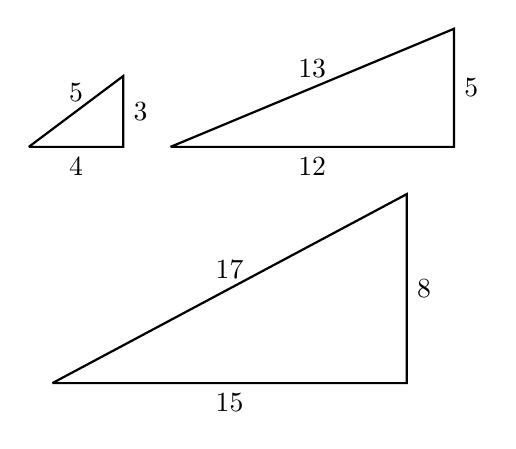
\begin{tikzpicture}[thick, scale=0.30]
        \draw (0,0) -- (4,0) node[midway,below]{$4$}
        -- (4,3) node[midway,right]{$3$}
        -- (0,0) node[midway,above]{$5$};
        \draw (6,0) -- (18,0) node[midway,below]{$12$}
        -- (18,5) node[midway,right]{$5$}
        -- (6,0) node[midway,above]{$13$};
        \draw (1,-10) -- (16,-10) node[midway,below]{$15$}
        -- (16,-2) node[midway,right]{$8$}
        -- (1,-10) node[midway,above]{$17$};
    \end{tikzpicture}
\end{center}

我们为何确信此定理成立?这个极其实用的结论,你可能在数学课堂上(或日常生活中不经意地)多次运用过。但你有没有思考过为什么这是真的?你会如何向持怀疑态度的朋友解释呢?这正是\textbf{数学证明}试图完成的:对事实给出清晰而严谨的解释。寻求证明背后的原因也十分有意义,它具有两重含义:即确保我们认为为真的事情确实为真,又避免要使用时进行重复论证。一旦(令人信服地)完成毕达哥拉斯定理的证明,后续只需引用定理名称即可;我们已经证明过了,所以无需再次证明。

那么,究竟什么构成了证明?如何判断解释是否足够清晰和简洁?一般来说,这些问题本身具有相当的复杂性,这也使得数学兼具科学与艺术的双重属性。尽管处理的都是严谨客观的事实,但如何有效地推理并以令人信服的方式呈现,实则是一门艺术。

\subsubsection*{``证明''范例}

让我们一起看几个``证明''的例子,看看它们是否足够好。(我们现在先说``证明'',稍后为其下更精确的定义。)这里是第一个:

\begin{proofs}{``证明'' 1.}
    构造边长为 $a+b$ 的正方形。在正方形内部放置 $4$ 个全等的直角三角形,形成边长为 $c$ 的内接正方形。

    \begin{center}
        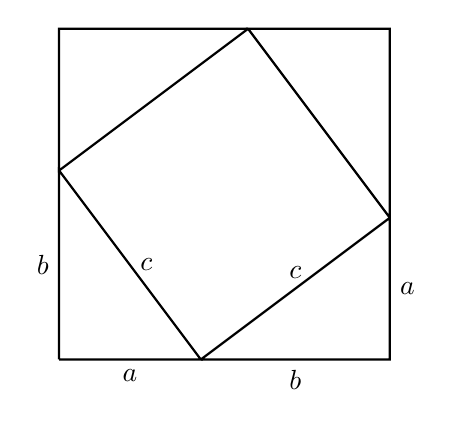
\begin{tikzpicture}[thick, scale=0.6]
            \draw (0,0) -- (3,0) node[midway,below]{$a$}
            -- (0,4) node[midway,right]{$c$}
            -- (0,0) node[midway,left]{$b$};
            \draw (3,0) -- (7,0) node[midway,below]{$b$}
            -- (7,3) node[midway,right]{$a$}
            -- (3,0) node[midway,above]{$c$};
            \draw (7,3) -- (7,7)
            -- (4,7)
            -- (7,3);
            \draw (4,7) -- (0,7)
            -- (0,4)
            -- (4,7);
        \end{tikzpicture}
    \end{center}

    大正方形的面积可以用两种方式表示:直接应用正方形的面积公式,或者把内接正方形和四个直角三角形的面积加起来。因此,下面这个等式一定成立。
    \[(a+b)^2=c^2+4\cdot\frac{ab}{2}=c^2+2ab\] 
    将左边表达式展开,然后两边同时消掉同类项可得 
    \[a^2+\cancel{2ab}+b^2=c^2+\cancel{2ab}\] 
    所以,$a^2+b^2=c^2$ 成立。
\end{proofs}

上面的证明是否具有说服力?每一步是否合理?可能你现在还太不确定,那么让我们接着看一下此定理的另一种``证明''。

\begin{proofs}{``证明'' 2.}
    假设毕达哥拉斯定理成立。绘制直角三角形,并过直角顶点向对应边做高。如下图所示:
    \begin{center}
        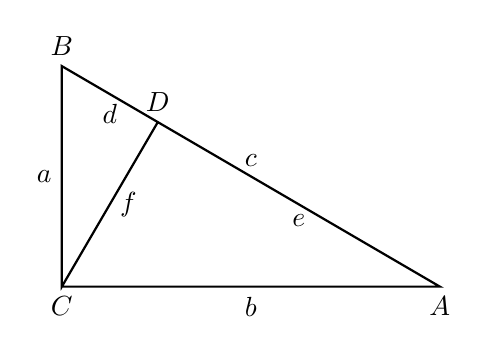
\begin{tikzpicture}[thick, scale=0.8]
            \coordinate (C) at (0,0);
            \coordinate (A) at (6,0);
            \coordinate (B) at (0,3.5);
            \coordinate (D) at (1.523316, 2.611399);
            \draw (C) node[anchor=north]{$C$}
            -- (A) node[anchor=north]{$A$} node[midway,below]{$b$} 
            -- (B) node[anchor=south]{$B$} node[midway,above]{$c$}
            -- (C) node[midway,left]{$a$}
            -- (D) node[anchor=south]{$D$} node[midway,right]{$f$}
            -- (A) node[midway,below]{$e$} 
            -- (D)
            -- (B) node[midway,below]{$d$};
            \rightAngle{B}{D}{C}{0.3};
        \end{tikzpicture}
    \end{center}
    因为毕达哥拉斯定理成立,所以我们可以将其应用到图中的三个直角三角形中,即三角形 $ABC, BCD, ACD$。(定义 $e = c-d$)可得
    \begin{align*}
        a^2 &= d^2 + f^2 \\
        b^2 &= f^2 + e^2 \\
        c^2 &= a^2 + b^2
    \end{align*}
    将前两个方程相加,再用代入第三个方程,可得
    \[c^2 = d^2 + e^2 +2f^2\]
    注意到 $\angle ABC$ 与 $\angle ACD$ 相等,因为它们都与角 $\angle CAB$ 互余,由此可知 $\triangle CDB$ 与 $\triangle ADC$ 相似。(此处默认你对平面几何有所了解。)由此可得 $\frac{e}{f} = \frac{f}{d}$,因此 $f^2 = ed$。我们可以将其带入上面的公式替换 $f^2$,结果如下:
    \[c^2 = d^2+e^2+2de = (d+e)^2\]
    两边同时开方(已知 $c,d,e$ 都是正数)可得 $c = d+e$,根据边长 $d$ 和 $e$ 的定义,这显然成立。因此,假设毕达哥拉斯定理成立是正确的。
\end{proofs}

这个证明怎么样?有说服力吗?表述清晰吗?在确定什么构成``正确的''或``良好的''证明之前,让我们再考察一个``证明''。

\newpage

\begin{proofs}{``证明'' 3.}
    观察下图
    \begin{center}
        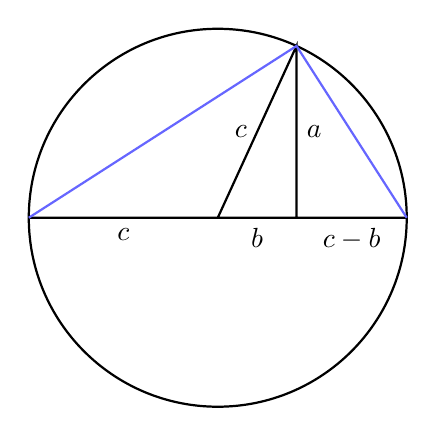
\begin{tikzpicture}[thick, scale=0.4]
            \coordinate (O) at (0,0);
            \coordinate (A) at (-6,0);
            \coordinate (B) at (6,0);
            \coordinate (C) at (2.5,0);
            \coordinate (D) at (2.5,5.45435);
            \draw (O) circle (6);
            \draw (A) -- (O) node[midway,below]{$c$}
            -- (C) node[midway,below]{$b$}
            -- (B) node[midway,below]{$c-b$}
            -- (C)
            -- (D) node[midway,right]{$a$}
            -- (O) node[midway,left]{$c$};
            \draw[color=blue!60] (A) -- (D) -- (B);
            \rightAngle{B}{C}{D}{0.6};
        \end{tikzpicture}
    \end{center}  
    由图形可得 $\frac{a}{b+c} = \frac{c-b}{a}$,因此 $a^2 + b^2 = c^2$。
\end{proofs}

这个证明对你来说合理吗?最后,还有一个需要思考的``证明''。

\begin{proofs}{``证明'' 4.}
    毕达哥拉斯定理必然成立,否则我的老师一直在欺骗我。
\end{proofs} 

\subsubsection*{讨论}

在继续阅读之前,建议你先独立思考这四个``证明'',也可与同学或朋友讨论一下。你认为什么构成``正确''的证明?清晰性和易读性重要吗?它会影响证明的``正确性''吗?

从历史角度看,数学证明的撰写历经多年演变,已经对什么构成``正确''的证明形成了普遍共识:

\begin{itemize}
    \item 从数学角度来说,证明中的每一\emph{步}、每一个逻辑推理和命题均需保持\emph{数学有效性},这一点非常重要。
    \item 同样重要的是,证明撰写者需(合理地)阐明陈述如何源于前置工作或外部知识。
\end{itemize}

这种对\emph{真理性}的要求,使得已建立的数学论证,可以通过逐步验证确认每个命题是\textbf{对}还是\textbf{错}。难点在于对清晰表达的界定。某种程度上,这就像最高法院大法官波特·斯图尔特(Justice Potter Stewart)对淫秽的著名定义:``见之即明''。

下面从清晰性和正确性两方面评估这四个论证:

\textbf{清晰性:}

\begin{itemize}
    \item ``证明'' 1 和``证明'' 2 表述清晰。明确解释了操作动机与依据。不仅给出了每个方程式的来源,还辅以图示说明。
    
    请注意,``证明'' 1 确实依赖一些基本的先验知识,例如基本代数运算以及三角形和正方形的面积公式,但这没有问题。

    同样地,``证明'' 2 依赖相似三角形的一些知识以及它们边长之间的关系。撰写者明确指出了这一点,所以有兴趣的读者可以查阅相关知识点。如果撰写者没有指出,读者可能会感到困惑,不知道如何得出这个结论。
    \item ``证明'' 3 写得非常糟糕!它没有提供任何解释。这使得读者很难确定其结论是否正确。尽管其中包括一张图片,但并没有解释\emph{为什么}要画一个三角形的外接圆,或者为什么能从图中得出所述方程。
    \item ``证明'' 4 虽语法正确,但并未提供任何\emph{解释}!
\end{itemize}

由此可见,对于一个逻辑正确且书写良好的证明来说,``证明'' 4 无疑是一个糟糕的证明。``证明'' 1 和``证明'' 2 仍在候选之列,因为它们至少写得很清楚。``证明'' 3 目前看可能不是一个好的证明;也许它确实包含正确的结论,只是需要更好的解释。通过重写可以使其变成一个良好的\emph{证明}。

让我们再来分析一下这四个论证的逻辑正确性:

\textbf{正确性:}

\begin{itemize}
    \item ``证明'' 1 大部分都很好。正确应用了正方形和三角形的面积公式,并且其代数运算也正确。但是我们怎么知道其所描述的过程 —— 将给定四个三角形放入正方形内 —— 会构建一个边长为 $c$ 的内接正方形?证明中只是说这样\emph{可以},但并未真正说明\emph{为什么可以}。不过,除此疏漏外,这个证明写得很好而且是正确的。
    
    (你能证明里面的形状实际上是正方形吗?看一下它的角度:你能说明为什么它们都是直角吗?)
    \item 很遗憾,``证明'' 2 完全是错误的!尽管它所做的每一个逻辑步骤都遵循前一个步骤。例如,假设我们以这种方式设置三角形,我们可以正确推断出 $\triangle CDB$ 和 $\triangle ADC$ 是相似三角形。然而,为什么我们可以在一开始就\emph{假设}该定理为\textbf{真}呢?总的来说,这不正是我们在证明中试图实现的目标吗?这是一个关键缺陷。\textbf{假设一个事实并从中推断出某些结论为真并不能得出原始假设必然为真。}
    
    如果这种方法有效,我们可以``证明''任意命题!举个例子:你如何看待以下证明 $0 = 1$ 的``证明''?
    \begin{proof}
        假设 $0 = 1$。那么,根据 $=$ 的对称性,$1 = 0$ 也是成立的。将这两个方程相加可得 $1 = 1$,这显然为真。因此,$0 = 1$ 是一个有效的假设,因此它一定为真。
    \end{proof}
    你看出上面证明与``证明'' 2 有什么相似之处吗?它们使用了同样有缺陷的推理:假设一个事实,做了一些工作得到我们已知为真的其他事实,然后断言假设的事实也必然为真。
    \item 对于``证明'' 3 ,大多数数学家会说这是一个``糟糕的证明'',尽管其透露出的结论似乎都是正确的。我们说``透露出''是因为,如果没有任何文字解释思路,就无从知晓撰写者想表达什么!然而,不得不说,完美证明的核心思路就包含其中。
    
    从图中,你可以证明方程 $\frac{a}{c+b} = \frac{c-b}{a}$ 一定成立。(提示:使用相似三角形!)进而可以推导出 $a^2 + b^2 = c^2$。

    你能写一些文字来配合图形,将其改写为良好的证明吗?
    \item 最后,几乎每个逻辑正常的人(我们希望如此!)都会说``证明'' 4 根本不是一个证明,无论做出这样的陈述多么方便。
\end{itemize}

综上,``证明'' 1 是一个良好的证明。在 4 个证明中,``证明'' 1 写得最清楚,逻辑也最正确。我们可以将其视作\textbf{证明}。``证明'' 2 是完全错误的,尽管它表述得非常清楚。``证明'' 3 包含正确的思路,但缺乏清晰的表述。``证明'' 4 离证明十万八千里,毫无讨论价值。

\subsubsection*{问题}

在继续讨论其他主题之前,留下一个问题供你思考:给定三个正数 $a,b,c$ 满足 $a^2+b^2=c^2$,是否一定存直角边长为 $a,b$ 斜边长为 $c$ 的直角三角形?倘若存在,你会如何着手构造它?若不存在,原因何在?


% !TeX root = ../../../book.tex
\subsection{质数时间}\label{sec:section1.1.2}

当我们讨论证明这个主题时,让我们看一下另一个重要定理的证明。首先简要回顾\emph{质数}的定义。

\subsubsection*{定义、示例与应用}

\begin{definition}\label{def:prime}
    若正整数 $p>1$ 的正因子只有 $1$ 和 $p$ 本身,则称 $p$ 为\dotuline{质数}。非质正整数称为\dotuline{合数}。
\end{definition}

质数在数学的诸多分支中都具有核心地位,而不仅限于研究整数性质的\textbf{数论}领域。数学中最著名的\textbf{猜想}(迄今为止既没有被证明也没有被证伪的命题)当数\emph{黎曼猜想}。该猜想已被证实与质数在整数中的分布规律密切相关,相关研究著作浩如烟海。此外,大多数现代密码学的基础都是大质数的乘积特性 --- 将两个大质数相乘容易,但将乘积逆向分解为两个大质数却极为困难。现在你知道了:每当你用信用卡在 iTunes 上购买歌曲时,背后的计算机系统都会将两个大质数相乘!

前几个质数依次为 $2, 3, 5, 7, 11, 13, 17, 19, 23,\dots$(注意,$1$ 不满足定义)。那么质数有多少个?相邻质数相距多远?是否存在分布规律?这些问题虽引人入胜却极难解答(有时甚至是不可能的!)。本节将聚焦其中一个问题:质数是否有无穷多个?

\subsubsection*{定理与证明}

\begin{theorem}[质数无穷性]
    质数有无穷多个。
\end{theorem}

\begin{proof}
    假设质数有有限多个,按升序列出为:$p_1, p_2, p_3, \dots, p_k$,所以 $p_k$ 为最大质数。现构造新数
    \[N = (p_1 \cdot p_2 \cdot p_3 \cdot \dots \cdot p_k) + 1\]
    $N$ 必有质因子。然而,它一定不能被 $p_1$ 或 $p_2$ 或 $\dots$ 或 $p_k$ 整除,因为根据 $N$ 的定义,除以上述质数都会得到余数 $1$。因此 $N$ 可以被列表中未列出的其他质数整除。

    如果 $N$ 是合数,那么我们就发现了一些新质数 $p < N$,它不在所有质数列表中。
    
    如果 $N$ 是质数,那么我们就得到了一个新质数 $N > p_k$,所以 $p_k$ 实际上并不是最大的质数。无论哪种情况,我们必然有一个新的质数不在给定的 $k$ 个质数的列表中,这与有限性假设矛盾。因此,质数必定有无穷多个。
\end{proof}

对于这个``证明''你怎么看?是否令你信服?这里的论证方式与我们迄今为止看到的其他论证方法有所不同。不妨尝试向同学解释本节的证明与上一节毕达哥拉斯定理的``证明 1''有何不同。我们很快将揭示:此处的``证明''实际上是一个完全正确的\emph{证明}!


% !TeX root = ../../../book.tex
\subsection{无理取闹}

现在让我们讨论另一类数字:\textbf{有理数}。你可能知道``分数''、``商''或``比率''指的都是有理数。

\subsubsection*{定义与示例}

以下是\emph{有理数}的精确定义:

\begin{definition}
    实数 $r$ 是\dotuline{有理数}当且仅当它可以表示为两个整数之比 $r = \frac{a}{b}$,其中 $a$ 和 $b$ 均为整数(且 $b \ne 0$)。

    一个实数不是有理数就是\dotuline{无理数}。
\end{definition}

定义并未规定有理数必须具有唯一的表示形式;它只要求有理数至少有一种定义中的表示。例如,$1.5$ 是有理数,因为 $1.5 = \frac{3}{2} = \frac{12}{8} = \frac{30}{20}$ 等等。这一定义具有完备性:一个实数不是有理数就是\textbf{无理数},\emph{非}有理数,即不存在将其表示为整数之比的形式。你可能知道 $\sqrt{2}$ 是一个无理数,但如何\emph{证明}这一点呢?请尝试自行证明。我们稍后会重新讨论这个问题(见示例 \ref{sec:section4.9.4})。其他常见的无理数还包括 $e, \pi, \varphi$ 以及 $\sqrt{n}$(其中 $n$ 为正整数且不为完全平方数)。

\subsubsection*{问题}

基于有理数/无理数的定义,我们可以探讨无理数的组合能否产生有理数。请尝试独立解答以下问题:若答案为``是'',请举例说明;若答案为``否'',请解释其不可能性。

\begin{enumerate}
    \item 是否存在无理数 $a$ 和 $b$ 使得 $a \cdot b$ 为有理数?
    \item 是否存在无理数 $a$ 和 $b$ 使得 $a + b$ 为有理数?
    \item 是否存在无理数 $a$ 和 $b$ 使得 $a^b$ 为有理数?
\end{enumerate}

你能构造出具体例子吗?事实上,这三个问题的答案均为``是''!前两问较为简单,第三问则略微棘手。

以下我们给出第三问的证明。有趣的是,该证明并不直接给出满足条件的 $a$ 和 $b$;而是将可能性缩小至两种情形,并证明其中\emph{必有}一种成立。听起来很有趣,对吧?我们来试试吧。

\begin{proof}
    已知 $\sqrt{2}$ 为无理数。考虑数字 $x = \sqrt{2}^{\sqrt{2}}$。有两种可能的情况:
    \begin{itemize}
        \item 若 $x$ 为有理数,则令 $a = \sqrt{2}, b = \sqrt{2}$ 即满足条件。
        \item 若 $x$ 为无理数,则令 $a = \sqrt{2}^{\sqrt{2}}, b = \sqrt{2}$,此时
        \[a^b = \Bigg(\sqrt{2}^{\sqrt{2}}\Bigg)^{\sqrt{2}} = \Big(\sqrt{2}\Big)^{\sqrt{2} \cdot \sqrt{2}} = \Big(\sqrt{2}\Big)^2 = 2\]
        $2$ 为有理数。
    \end{itemize}
    无论何种情形,均可找到无理数 $a$ 和 $b$ 使得 $a^b$ 为有理数。因此,这样的数字对必然存在。
\end{proof}

你觉得这个证明怎么样?是否有说服力?它以明确的``是''回答了上面的第三问,但未指明具体\emph{哪一对} $a, b$ 是正确的,而是告诉我们其中必有一对满足。(事实证明 $\sqrt{2}^{\sqrt{2}}$ 确为无理数,但这一事实需要额外证明。)

还有很多其他具体例子可以回答这个问题。你能想出任何其他方法吗?(提示:尝试使用 $\log_{10}$ 函数……)


\newpage
% !TeX root = ../../../book.tex
\section{大罗洞观}\label{sec:section1.2}

% !TeX root = ../../../book.tex
\subsection{简单符号}

\subsubsection*{数学是门语言}

尽管看上去全是符号(那些写得密密麻麻的教科书所呈现的),但数学不仅仅是我们纸上所用符号的集合。英语基于一组固定的符号(字母表中的 26 个字母加上常见的标点符号,如句点、逗号和括号),但我们可以以特定的方式将这些符号组合在一起,并遵循一定的标准和约定,创作出有意义的单词、短语、句子、段落等;从本质上讲,英语和任何其他语言一样,通过符号集合以及组织这些符号的规则集合,来传达含义。同样的概念也适用于\emph{数学语言}:有一组符号和一组作用于这些符号的规则。

一个区别是,我们在数学中使用的符号集合可能相当大,具体取决于当前讨论的数学分支。数学结构多样性的一个重要部分是我们总是可以创建和定义要使用的新符号。通常,这样做只是为了使内容更简短、更易于阅读。

数学与其他语言之间的另一个主要区别是,我们仔细选择如何\emph{定义}我们的单词及其表达的概念。通常,数学家的大多数争论都围绕定义展开。这可能会令你感到惊讶;似乎数学家就证明和猜想进行辩论才更合理,甚至数学家居然会辩论都是一个新奇的想法!为新发现的概念选择正确的定义和术语是数学发现和阐述的重要组成部分,因为这有助于发现者/发明者向其他感兴趣的人解释他/她的想法。(没有这个过程,数学就不会进步,只是一群孤立的人试图自己发现真理。)

口语的情况与此类似,但似乎没有那么极端。例如,如果你对你的朋友说,``我饿了'',或者``我感觉有点饿了'',或者``天哪,我饿死了'',他们听到的基本上是相同的信息,并给出大致相同的回应。然而,在数学中,我们的定义要精确得多,并且不包含口语允许的细微差别。当然,这两种哲学各有优缺点,但在数学中,我们尽可能追求精确,因此我们希望我们的定义准确且稳定。尽管如此,我们可以掌控这些定义是什么!这就是为什么关于定义的争论在数学世界中如此普遍:为手头的概念选择正确的定义可以使未来使用这些概念的工作变得更加容易和方便。

\subsubsection*{恰当选择定义}

作为一个具体的例子,让我们回到上一节中看到的质数的定义\ref{def:prime}。它说的是:

\begin{definition}
    如果大于 $1$ 的正整数 $p$ 其正因子只有 $1$ 和 $p$,则称 $p$ 为\dotuline{质数}。非质正整数称为\dotuline{合数}。
\end{definition}

这个定义似乎没有什么问题,不是吗?也许你会用不同的措辞或更简洁的表达或使用不同的可变字母或其他,但最终的信息是相同的:质数是具有特定属性的某种类型的数字。而你选择写出该特定类型的数字是什么(大于 $1$ 的正整数)以及该属性是什么(没有除 $1$ 和它本身以外的正因子),你将获得等效的定义。

不过,这个定义背后存在一些微妙的问题:为什么它是那种特定类型的数字?为什么我们如此关心这个特殊的属性——只能被 $1$ 和它本身整除?如果定义略有不同怎么办?事情真的会有那么大的改变吗?我们将用另一个问题来解决这些问题:你如何看待以下质数的替代定义?

\begin{definition}\label{def:prime2}
    如果小于 $-1$ 或大于 $1$ 的整数 $p$ 其正因子只有 $1$ 和 $p$,则称 $p$ 为\textbf{质数}。
\end{definition}

你注意到细微的差别了吗?所有符合之前``质数''定义的数字仍然符合这个定义,但现在负数也适用!具体来说,给定任意数字 $p$ 在旧定义下是质数,$-p$ 现在在新定义下也是质数。这是一个合理的想法吗?负质数有什么问题?

质数的第三个定义怎么样?

\begin{definition}\label{def:prime3}
    如果正整数 $p$ 的正因子只有 $1$ 和 $p$,则称 $p$ 为\textbf{质数}。
\end{definition}

(请记住,按照惯例,$0$ 既不是正数也不是负数。)现在,负数会超出范围,但 $1$ 符合此定义。这合理吗? $1$ 的唯一正因子是 $1$ 和...它本身,对吗?

这就是可能引发争论的地方:也许你不介意让 $1$ 成为质数,但你的朋友会强烈反对。好吧,如果没有确凿的理由,就没有办法说你们中任何一个都是错的,真的;你只是对术语做了不同的选择,它们都没有改变 $1$ 的唯一正因子是 $1$ 和它本身这一固有属性。类似地,请考虑一下:无论你称它们为凉鞋、拖鞋还是人字拖,事实仍然是这些类型的鞋子适合在海滩上穿。

然而,考虑到历史的后见之明和新的愿望,通常一个特定的定义被认为更加合适。未来,我们将研究质数分解,这是一种将每个(正)整数写为质数乘积的方法。例如,$15 = 3 \cdot 5$, $12 = 2 \cdot 2 \cdot 3 = 2^2 \cdot 3$ 和 $142857 = 33 \cdot 11 \cdot 13 \cdot 37$ 都是质因数分解。

这些因数分解也有一个特殊的性质:一般来说,正整数的质因数分解是\textbf{唯一的}!也就是说,只有一种方法可以将正整数写为质数的乘积(因为我们将因子的不同排序视为同一事物,所以 $105 = 3 \cdot 5 \cdot 7$ 和 $105 = 7 \cdot 3 \cdot 5$ 是相同的因数分解)。我们将使用上面给出的第一个定义严格证明这一点。如果我们使用第二个定义或第三个定义会怎么样?这种唯一性还存在吗? 为什么这种唯一性如此重要?最终,结论是,定义应该由逻辑和实用性驱动,并且这可能会随着时间的推移而改变并引发一些争论。

\subsubsection*{数学家的学习模式}

建立清晰准确的定义的另一个好处是你可以像思想者一样获取知识和理解;人类学习的一个主要方面涉及通过日常经验识别模式,接着将想法、概念、词语、事件与这些模式联系起来。然后,人们可以使用这些模式来预测抽象的想法、概念和事件并对其进行理论化。

例如,研究表明,人类婴儿最初缺乏\emph{物体存继性}概念,随着时间的推移逐渐发展起来。如果你给孩子看一个他们喜欢的彩色玩具,然后把它藏在纸箱下面,孩子不太明白这个玩具仍然存在,只是看不见了。他/她会表现得好像该物体不再存在一样。然而,在某些时候,我们知道这不是真的,我们视野之外的物体仍然存在。这究竟是如何发生的?也许是我们见识到许多此类事件的模式,其中一个物体``消失'',然后我们又找到它。

更好的例子可以在自然科学中找到,它们说明了模式识别和抽象思维的另一个方面,这是极其重要的,特别是在数学和科学领域。我们可以想象,尼安德特人不知何故知道,每当他们拿起一块岩石并将其保持在一定距离,然后松开时,岩石就会掉到地上。这种情况可能一次又一次地发生,所以他们``明白''这种现象是自然的必然产物。在发生足够多的事件之后,人们很可能明白这种情况总会发生,或者至少,任何没有发生的情况都会引起极大的困惑和恐惧。(正是这种情绪反应可能有助于解释火山爆发等罕见但强烈的事件如何导致古代文明将此类事件归咎于``神之愤怒'')。

对事件的观察并没有使史前人类进一步理解\emph{为什么}岩石总是会掉落到地面,或者能够\emph{解释}为什么它每次都必然发生。几千年后,人们才开始思考这种现象为何发生以及如何发生,更长时间之后,艾萨克·牛顿(Isaac Newton)最终提出了一个试图解释重力行为的模型(最终为此类现象命名)。有人说,即使是现在,我们仍然没有弄清楚它到底是如何运行的。(如果你好奇的话,可以上网搜索``循环量子引力''并尝试理解这一点)。

正是这种思维上的抽象飞跃——从对某种模式的观察到对该模式的认识论理解——从最好的意义上来说,是真正具有好奇心和智慧的思想家、真正的科学家的特征。你认为谁是更好的昆虫学家:贪婪的读者,他已经记住了世界上所有目前已知的甲虫种类,或者实验室科学家,他检查了多种物种,可以采集新标本并对其分类为甲虫还是非甲虫?这在某种程度上是一个引导性问题,但要点是:\emph{理解}定义及其背后的动机比简单地了解一堆满足某个定义的\emph{实例}要有益得多。

可以说,这对数学更为重要。你能想象一个数学家不知道质数是什么,只能凭记忆列出前 100 个质数并对此沾沾自喜吗?当然不是!数学研究的美妙、通用和魅力部分在于我们检查模式和现象,然后选择如何做出与这些模式相关的适当定义。然后,我们利用对这些模式的新理解来对其他模式和现象做出严格精确的预测。彻底理解定义或概念可以提高预测能力,并且比仅仅了解该定义/概念的示例更为有效。



% !TeX root = ../../../book.tex
\subsection{正确撰写}

数学的另一个有趣的方面是,尽管它本身就是一种语言,但我们依赖外部语言来传达我们所拥有的数学思想和见解。尝试在不使用任何单词的情况下重写我们之前看过的定义和证明。这很难,不是吗?因此,我们希望用来传达数学思想的书面语言遵循与我们所写的数学``句子''相同的标准:我们希望它们\emph{精确}、\emph{合乎逻辑}且\emph{清晰}。

现在,为这三个词下一个精确、合乎逻辑且清晰的定义本身就是一项艰巨的任务。然而,我们都认同理想的证明应该具备:

\begin{itemize}
    \item \textbf{精确性:}任何陈述都不应是不真实的或可以通过多种方式解释从而导致真相需要商榷;
    \item \textbf{逻辑性:}每一步都应遵循先前的步骤,并有适当的动机和解释;
    \item \textbf{清晰性:}步骤间应该用正确的语法连接和描述,帮助读者了解发生了什么。
\end{itemize}

让我们检视几个无视这些标准并且在某种程度上不符合我们迄今为止的证明定义的``证明''。

\subsubsection*{糟糕``证明''\#1}

首先,我们来一个 $1=2$ 的``证明'',我们知道这肯定有问题。你能找到哪里出错了吗?它违反了哪个标准?精确性、逻辑性还是清晰性?

\begin{proofs}{``证明''}
    假设有两个实数 $x$ 和 $y$,考虑如下等式:
    \begin{align*}
        x &= y \\
        x^2 &= xy &\text{两边同时乘以\ } y\\
        x^2-y^2 &= xy-y^2 &\text{两边同时减去\ } y^2\\
        (x+y)(x-y) &= y(x-y) &\text{因式分解} \\
        x + y &= y &\text{两边同时消去\ } (x-y)\\
        y + y &= y &\text{因为第一行给定\ } x=y\\ 
        2y &= y \\
        2 &= 1 &\text{两边同时除以\ } y
    \end{align*}
\end{proofs}

这里的问题在于\emph{精确性}。对第四行进行因式分解后,除以公因数 $(x - y)$ 即可得到第五行,这似乎既方便又明智;然而,第一行告诉我们 $x = y$,所以 $x-y = 0$,\textbf{除以零是不允许的}!使用变量 $x$ 和 $y$ 只是一种让你失去踪迹并掩盖除以零的方法。(说到这里,为什么不能除以零?你能想出一个合理的解释吗?从乘法的角度思考一下。)

\subsubsection*{糟糕``证明''\#2}

这是类似``事实''的另一个证明,即 $0 = 36$。

\begin{proofs}{``证明''}
    考虑方程 $x^2+y^2 = 25$。整理并分离 $x$ 可得
    \[x = \sqrt{25-y^2}\]

    两边加3再同时平方得
    \[(x+3)^2=\left(3+\sqrt{25-y^2}\right)^2\]

    请注意,$x = -3$ 和 $y = 4$ 是原方程的解,所以最终的方程也应该是成立的。将这组解代入 $x$ 和 $y$ 可得
    \[0 = (-3+3)^2 = (3+\sqrt{25-16})^2 = (3+3)^2 = 36\]
    
    因此,$0 = 36$。
\end{proofs}

到底发生了什么?你能发现不合逻辑的步骤吗?如果我们使用最后选择的变量 $x$ 和 $y$ 的特定值重写证明步骤,也许会有所帮助:

\begin{align*}
    (-3)^2+4^2 &= 25 \\
    -3 &= \sqrt{25-4^2} \\
    (-3+3)^2 &= \left(3+\sqrt{25-4^2}\right)^2 \\
    0 &= 36
\end{align*}

现在很明显了,不是吗?对方程两边取平方根存在一个问题,它取决于 $(-x)^2=x^2$ 这一事实。

当我们解 $z^2=x^2$ 这样的方程时,必须牢记这个方程有两个根:$z = -x$ 和 $z = x$。因此,从方程开始并对两边进行平方是一个完全合乎逻辑的步骤(所得方程的真值与原方程的真值\emph{一致}),但反之却是一个不合逻辑的步骤(平方方程成立并不\emph{一定}等于平方根方程也成立)。这是一个带有\textbf{条件陈述}或\textbf{逻辑蕴涵}的问题,我们稍后会详细讨论这些概念(第 4.5.3 节)。现在,我们可以用下面的代码来总结这个概念:
\[\text{如果\ } a=b, \text{则\ } a^2=b^2, \text{反过来,如果\ } a^2=b^2, \text{则\ } a=b \text{\ 或\ } a=-b\]

这说明了为什么在上面``证明''中从 $x^2+y^2 = 25$ 到 $x = \sqrt{25-y^2}$ 这步是不合逻辑的:当有两种可能的选择时,我们立即假设平方根的一种特定选择。如果我们选择负平方根,会发生什么?试着将第二步替换为 $-x = \sqrt{25-y^2}$ 并重写证明,在最后对 $x$ 和 $y$ 使用相同的值。发生了什么? 如果你用 $x = 3, y = -4$ 代替呢?或者 $x=-5, y=0$ 呢?你能描述一下如何确定何时应该使用正根 $x$ 何时应该使用负根 $-x$ 吗?

\subsubsection*{数学使用``兼或''}

既然``或''这个词已经出现,我们先提一下上面句子中\emph{或}的使用。当我们说 ``$a = b$ 或 $a = -b$'' 时,我们的意思是,这两个陈述中\emph{至少}有一个必须为真,甚至可能两者都为真。现在,如果 $a \ne 0$ 且 $b \ne 0$,则只有其中一种结论性陈述可以为真;也就是说,在这种情况下,只有一个根(正或负)是正确的,而不是两者都是正确的。然而,如果 $b = 0$,那么两个结论性陈述说的是同样的事情,$a = 0$,因此规定\emph{或}意味着只有一个陈述可以为真并且不允许它们都为真,这是不合逻辑的。在其他情况下,这种区别会产生更显着的差异。

例如,如果你在餐厅点了一份三明治,服务员问:``您想要薯条还是土豆沙拉?'',这可以理解为,你可以选择其中一项,但不能同时选择两者。这就是\textbf{异或}的示例,因为它阻止你选择两个选项。或者,如果你忘记带书写工具去课堂,准备用老方法记笔记于是询问你的朋友,``我可以借用您的铅笔或钢笔吗?'',这可以理解为,你实际上并不关心提供两个选项中的哪一个,只要至少有一个可用即可。也许你的朋友两者都有,而且其中任何一个都可以。这是\textbf{兼或}的示例,并且这是所有数学示例中假定的解释。

\subsubsection*{不清楚的论证}

最后两个糟糕的``证明''问题在于精确性和逻辑正确性。我们要求良好证明的第三个条件是\emph{清晰}:我们希望文字能够解释证明者在每个步骤中完成的工作以及为什么该工作是相关的。换句话说,我们不希望读者在任何时候停下来问:``这句话是什么意思?''或``那是从哪里来的?''或因困惑而产生的类似问题。如果有帮助的话,考虑写一个证明,向你班上的朋友、将要阅读你作业的评分者或智力相当的家庭成员解释它。重读你自己写的证明,并尝试预测可能出现的问题或可能要求你进行的澄清,然后通过重写来解决这些问题。

证明可能因为多种原因失败或不清晰,首当其冲的是,单词和句子可能无法正确解释证明的步骤和动机,这实际上可能是因为单词太多(使读者负担过重而模糊了证明)或因为单词太少(没有给读到者足够的信息)或者因为所选的词语令人困惑(没有正确解释证明)。这些是证明\emph{语言}的问题。

从数学上讲,就清晰性而言,可能会出现许多问题。也许证明撰写者突然引入一个变量,但没有说明它是什么类型的数字(整数、实数等),或者跳过几个算术/代数步骤,或者使用新的符号而没有提前定义它的含义...这些行为在技术上都没有错误或不合逻辑,但它们肯定会给读者带来困惑。你能想到其他原因让证明不明确吗?尝试想出一种基于语言的原因和一种基于数学的原因。

\subsubsection*{糟糕``证明''\#3}

让我们陈述一个关于多项式函数的简单事实,然后查阅关于该事实的``证明''。仔细阅读论证并尝试找出一些不清楚的句子或数学步骤。

\textbf{事实:}考虑多项式函数 $f(x) = x^4-8x^2+16$。对于任意 $x$,该函数都满足 $f(x) \ge 0$。

\begin{proofs}{``证明''}
    无论 $x$ 的值是多少,我们将其代入 $x$ 的函数 $f$ 中,都可以通过对多项式进行因式分解写出该函数的输出值,如下所示:
    \[f(x) = x^4-8x^2+16 = (x-2)^2(x+2)^2\]
    而任意数字 $z$ 一定要么小于 $-2$,要么大于 $2$,要么严格介于 $-2$ 和 $2$ 之间,要么等于其中之一。当 $z > 2$ 时, $z - 2$ 和 $z + 2$ 都大于 $0$,因此 $f(z) > 0$。当 $z < -2$ 时,两项都为负而负数的平方为正,所以 $f(z) > 0$。当 $-2 < z < 2$ 时,类似情况再次发生,当 $x = 2$ 或 $x = -2$ 时,其中一项为 $0$,所以 $f = 0$。因此,我们要证明的必然成立。
\end{proofs}

这个证明有什么可批评的地方呢?首先,它正确吗?精确吗?符合逻辑吗?清楚吗?哪里不清楚?试着找出那些有点不清楚的陈述,无论是语言上的还是数学上的,并尝试适当地修改它们。在不指出个别错误的情况下,下面提供了上述事实的更好、更清晰的论证。

\begin{proof}
    我们首先对函数 $f(x)$ 进行因式分解,将其视为变量为 $x^2$ 的二次函数
    \[f(x) = (x^2)^2-8x^2+16 = (x^2-4)^2\]
    接下来,我们可以因式分解 $x^2-4=(x+2)(x-2)$ 并将原函数重写为
    \[f(x) = \left((x+2)(x-2)\right)^2 = (x+2)^2(x-2)^2\]
    对于任意实数 $x$,都有 $(x+2)^2 \ge 0$ 且 $(x-2)^2 \ge 0$,因为平方结果一定非负。两个非负项的成绩依然非负,所以 对于任意实数 $x$, $f(x) = (x+2)^2(x-2)^2 \ge 0$。
\end{proof}

第一个``证明''和第二个``证明''有什么区别?你重写的证明也像第二个证明吗?

对第一个``证明''的批评之一是它没有完全解释 $-2 < x < 2$ 的情况;相反,它只是说发生了``类似''的事情,并没有实际执行任何细节。这是数学中的常见情况(证明的某些步骤``留给读者''),这是一种简便技巧,有时可以避免繁琐的算术/代数,并使阅读证明更容易、更快速、更愉悦。但是,要谨慎使用该技巧。作为证明撰写者,确保步骤确实有效非常重要,即使你不打算在证明中呈现它们;你应该向读者提供简短的摘要或提示,说明这些步骤实际上是如何运作的。此外,证明撰写者应尽量不要在对证明最终结果至关重要的步骤上使用此技巧。

在上面的特例中,完全跳过了因式分解的实际步骤,并且只是顺便提及了对 $-2 < x < 2$ 情况的分析,但这些都是证明的重要组成部分!从任何维度上来说,这都是一个简短的证明,展示这些步骤并不代表在简洁性或清晰性方面做出了巨大的牺牲。这再次呼应了证明撰写既是科学也是艺术的观点:选择何时将一些细节验证留给读者可能很棘手。 在这种特殊情况下,展示所有步骤很重要。

尽管如此,我们给出的第二个证明要清楚得多。而且,完全摒弃了第一个``证明''中采用的分情况讨论技术!第一个``证明''中的一个情况存在清晰性问题,但我们没有简单地在重写版本中阐述细节,而是选择完全放弃该技术并使用更简短、更直接的证明。这并不是说第一个证明的技术是错误的。如果我们填补第一个``证明''论证中的空白,我们就会得到一个完全正确的证明。然而,该技术中的一些步骤是多余的。请注意,实际上 $-2 < x < 2$ 和 $x > 2$ 的情况在某种意义上是相同的:在这两种情况下,因子都满足 $(x - 2)^2 > 0$ 和 $(x + 2)^2 > 0$。事实上,第一种情况 $x<-2$ 也是如此!所以,当相同的最终观察结果对应于所有三个情况时,为什么要把论证分成三个不同情况呢?这种情况下,最好将它们合二为一(同样利用当 $x = 2$ 或 $x = -2$ 时,其中一个因子为 $0$ 的知识)。重申一遍,使用分开讨论技术当然没错。但是,它只会给证明增加不必要的长度。

我们在上面的段落中提到了术语``情况''和短语``分情况讨论'',但没有恰当定义或解释我们的意思。现在,我们想推迟对这些术语的讨论,直到我们在第 4 章中彻底讨论逻辑。不过,如果你渴望立即解决这个问题,可以跳到第 1.4.4 节并查看``匈牙利朋友''问题,其中包含一些复杂的分情况讨论。


% !TeX root = ../../../book.tex
\subsection{选择逻辑}

我们已经非常频繁地使用``逻辑''一词及其相关形式,但还没有充分解释其意思。我们意识到这似乎违背了我们迄今为止一直大力倡导的精确性和清晰性,但不幸的是,我们不得不承认,提供\emph{逻辑}的完整定义是极其困难的。

\subsubsection*{一场游戏}

如果你寻找对逻辑的启发式理解,可以尝试从``逻辑谜题''(如数独或数谜)入手来思考它。这些谜题/游戏从一开始就围绕定下的非常具体的规则构建的,然后向解谜者提供一个起始谜面,并期望解谜者严格遵守规则,直到解出谜题。例如,在数独中,规则是 1 到 9 中每个数字在每行、每列和 $3 \times 3$ 框中恰好只出现一次,解谜者需要综合各种情况在网格中放置越来越多的数字,不断缩小``潜在解''的范围,以找到起始谜面的唯一答案。这个解谜过程的一个重要方面是,任何时候都不要(自作聪明地)\emph{猜测};每一步都应该在考虑当前情况和谜题既定规则的情况下进行理性选择,并且在这个框架内,保证谜题是可以解决的(当然,要有足够的时间)。

数学逻辑在某些方面略有不同,但本质是一样的:都有既定的游戏规则,每一步都应该以这些规则和当前知识为指导,除此之外别无其他。这就是我们所说的撰写数学证明应该受\emph{逻辑}支配的意思:从一个真理到另一个真理,每一步都应该遵循约定的规则,并且只参考这些规则或已经证明的事实。我们在证明(以及一般的数学中)中玩的``游戏''或``谜题''并不像数独谜题那么清晰。然而,更令人困惑的是,有时我们会投身一场无法获胜的游戏,却丝毫没有意识到这一点!

这里``无法获胜的游戏''的想法来自 20 世纪奥地利逻辑学家、数学家库尔特·哥德尔 (Kurt Gödel) 的工作成果,这是一项令人震惊、使人惊奇但极其有力的结论。他的\emph{不完备性定理}反映出一个强大的逻辑系统内部的固有问题:有些\textbf{真实}陈述在该系统内却是不\emph{可证明}的。在这里,我们无法透彻详细地解释一些术语(即,\emph{逻辑系统}和\emph{可证明}),但希望你能看到这里出现了一些神奇的事情。这怎么可能呢?如果某事在数学中是\textbf{真的},我们不是应该能够以某种方式证明它是真的吗?否则我们怎么知道这是真的呢?

\subsubsection*{数学简史}

要回答这些自然而生的问题,让我们先退一步,回到数学的一个重要分支——逻辑的起源进行讨论。在整个讨论过程中要记住的一点是,我们无法完全解决出现的每个主题,这可能让人感到不满,我们理解这一点。数学之美部分在于,学习任何一个主题都会带来许多其他问题和概念需要思考,而这些问题和概念又可以通过更多的数学来解决。不过,背景很重要,就本书的背景而言,我们没有足够的时间和空间去讨论所有这些相关的主题。我们并不是试图向你隐瞒任何事情或掩盖某些问题;相反,我们只是在面对现实,确保我们不会强迫你阅读 10,000 页的完整数学史,只是为了理解我们的观点!

在你的数学生涯中,可能会进一步研究我们下面提到的许多数学家(以及他们所做的工作)。到那时,你将通过亲自动手实践从而对这个学科有更深入的理解和欣赏,你也将更有能力去解决其中的问题。而现在,我们仅仅是基于兴趣介绍这些数学家。数学有着丰富而有趣的历史,了解它会很有帮助!在这里,我们将尽力以简洁而有意义的方式来解读逻辑学——它的历史、动机和意义——使之与当前的背景相契合。

19 世纪中后期的数学家和哲学家首先研究了后来演变成现代逻辑的思想,他们对我们在这里试图研究的许多相同问题感兴趣:我们如何知道某件事是\textbf{真}的?我们如何才能表达这个真理呢?我们可以声明什么类型的``事件''为\textbf{真}或为假?这些数学家从根本上分解了数学语言,研究了如何以非常具体的方式组合一组固定的符号来创建更复杂的陈述,但从总体上看,这些陈述仍相当简单。这并不是要贬低他们的努力,毕竟,我们都必须从某个地方开始,而这些人是从头开始的。

首先进行的一项重大工作是探究算术的基础,或者说\textbf{自然数}($1,2,3,4,\dots$)的研究。就像欧几里得(Euclid)研究几何时,先通过建立一系列公认的真理或\textbf{公理},然后从这些给定的假设中推导出真理一样,意大利数学家朱塞佩·皮亚诺(Giuseppe Peano)建立了一套自然数公理,而其他人则从稍微不同的视角对这个主题进行了研究。与此同时,对真理及其证明严谨果断的欣赏,促使得大卫·希尔伯特和其他人提出了欧几里得公理的一些问题,尤其是平行公设。

这项关于几何和算术的工作自然引出了对数学其他领域的进一步、复杂的研究,以及对诸如实分析等领域热切地公理化尝试。卡尔·魏尔斯特拉斯(Karl Weierstrass)在研究这个主题时,提出了一些具有奇特属性的令人震惊的函数示例。例如,尝试定义一个处处不可微的连续函数。(如果你对微积分的这些术语不熟悉,请不用担心;总之,这很难。)最后,理查德·戴德金(Richard Dedekind)能够建立一个严谨的、逻辑的实数定义,完全由自然数推导出来,并且不依赖于必须存在数字连续体这种模糊的物理概念。

后来,这项研究稍微分支出来,变成了集合的研究。这个领域的许多基础工作是乔治·康托尔(Georg Cantor)在 19 世纪末期奠定的。他是第一个真正研究无限集理论的人,提出了无限有不同``大小''这一有争议的观点。也就是说,他证明了某些无限集严格大于其他无限集。这个想法在当时引起了极大的争议,以至于许多数学家都讨厌他!如今,我们意识到康托尔是对的。(这也让你提前窥探我们稍后在 7.6节中将会讨论的内容。举个有趣的例子:奇数集合和偶数集合当然一样大,但它们也和所有整数的集合一样大。然而,所有实数的集合严格大于二者!)

事实上,一些数学家对康托尔的发现感到相当震惊,甚至伟大的伯恩哈德·黎曼(Bernhard Riemann)一开始也认为集合论的发展将成为数学的祸害。但事实并非如此,从诞生起它就蓬勃发展,许多数学家致力于以正确的方式表示所有数学并理解数学的``基础''。某种程度上,你可以将集合论视为对所有数学家正在研究的基本对象的研究,最终,其方式类似于所有化学都是通过将元素周期表中的元素以越来越复杂的方式恰当地组合在一起来完成的。

这些主题的进一步发展是符号逻辑的研究,它比我们迄今为止提到的抽象概念更具体一些,而且我们在本书的开始章节中会频繁地研究这个领域的基本理念。该领域涵盖了如何将数学方程和符号与基于语言的符号和连词结合起来,以做出有意义的数学陈述,并可以通过证明来确认这些陈述的真实性。总的来说,这是数学的一个极其重要的组成部分,尤其是本书。个人观点当然比这更加细致和具体,但总的来说,大多数数学家的心态是,有许多数学真理等待被发现,我们花时间学习我们已经发现的真理,希望揭示更多真理。这就像一个巨大的考古挖掘,研究我们已经出土的骨头和文物将帮助我们预测我们在什么地方会发现什么类型的其他宝藏,以及如何寻找和挖掘。某种程度上,逻辑是从挖掘中一步一步抽象出来的过程:逻辑是对挖掘过程的研究。 它告诉我们如何真正利用数学知识并从中学习,并将其与其他知识相结合,从而证明更多的真理。

请注意,这不是一个精确的类比,抽象逻辑的研究要复杂得多。不过,就本书的目的而言,这是一种合理的思考逻辑的方式。我们将学习符号逻辑的一些基本原理和基本运算,并将这些知识应用到我们撰写证明的研究中。它将帮助我们真正理解证明是什么,它将指导我们构建要编写的证明,它将允许我们批判可能不正确的证明,并最终帮助我们理解数学作为一个整体是如何工作的。

\subsubsection*{逻辑应用:理论计算机科学}

逻辑思想和结果的一个非常重要的应用是计算机科学的发展和研究,特别是理论计算机科学和可计算性理论。这个特殊的数学分支最初是受大卫·希尔伯特二十三个问题——1900 年出版的数学界著名未解决猜想列表——中的第十个问题推动的。第十问题涉及解\textbf{丢番图方程(Diophantine Equations)}, 就是以下形式的方程
\[a_1x_1^{p_1}+a_2x_2^{p_2}+a_3x_3^{p_3}+\dots+a_nx_n^{p_n} = c\]
其中 $a_1, a_2, \dots, a_n$ 和 $c$ 都是给定的常数,$p_1, \dots, p_n$ 为给定的自然数,$x_1, \dots, x_n$ 为要求的使方程成立的变量。

给定这样一个方程,人们可能想知道是否存在解,如果存在,那么存在多少组解。 此外,如果我们给定常数 $a_i$ 和 $c$ 都是有理数,我们想知道是否可以确保存在一组解,其中所有变量 $x_i$ 也都是有理数。关于这个特定问题已经建立了一些理论成果,但是根据 1900 年的陈述,希尔伯特第十问题问的是,是否存在``一个过程,根据该过程可以经过有限数量的操作确定它''是否存在给定方程的解,其中所有变量 $x_i$ 都是有理数。尽管当时还没有算法这个术语的正确概念或定义,但希尔伯特要求的是一种\textbf{算法},该算法接受常数 $a_i$ 和 $c$ 的值,并根据是否存在所需属性的解输出 \textbf{True} 或 \textbf{False}。这个问题的一个重要部分是,该``过程''在输出答案之前执行有限数量的步骤。

一位名叫艾伦·图灵(Alan Turing)的英国剑桥大学学生几年后开始研究这个问题,他想到了一台物理机器,该机器将执行输出所提出问题的答案所需的步骤。他在随后的出版物中描述了他的发明,我们现在称之为\emph{图灵机},这是一种有趣的理论装置,可以用来回答形式逻辑中的一些问题,但也展现了构建现代计算机的许多想法。我们说它是一个理论装置,是因为它的定义的属性决定了它在物理上无法构建和操作,但它很好地处理了一些理论问题,包括前面提到的希尔伯特第十问题。更具体地说,当我们说某件事是可计算的,或者能够在有限数量的步骤中确定时,这台机器为我们的意思提供了正确的定义,这有助于建立正确的算法概念。如果我们在讨论可计算性话题时不提及阿隆佐·丘奇(Alonzo Church),那是不公平的,因为他与图灵同时在研究类似的问题。他们的名字一起出现在丘奇-图灵论文中,该论文将图灵机的工作原理与更理论化、基于形式逻辑的可计算性概念联系在一起。

\subsubsection*{我们将用逻辑做什么?}

虽然集合论和逻辑中的所有这些主题本质上都很有趣并且对数学非常重要,但总的来说,我们根本没有足够的时间和空间来详细讨论它们。相反,我们更关注在撰写和批判数学证明时使用的逻辑概念。

我们将考虑:

\begin{enumerate}
    \item 我们实际上可以陈述和证明什么类型的``事物'',
    \item 我们如何将我们已知为真的``事物''结合起来以产生更复杂的真理,
    \item 我们如何解释我们是怎样得出``事物''确实为真的结论。
\end{enumerate}

由于缺乏更好的术语,这里我们用``事物''一词,因为我们还没有\textbf{数学陈述}的正式定义,而这实际上是我们将要证明的``事物''的类型。从本质上讲,数学陈述是数学和语言中符号和句子的组合,可以验证为\textbf{真}或为\textbf{假},但不能同时既真又假或非真非假。那么,证明就相当于组织一系列步骤和解释,使用为真的数学陈述和句子将这些真理连接在一起,并最终产生特定陈述所需的真理。我们对逻辑的研究将解决如何组合这些步骤并确保我们的证明最终会导出对真理的正确评估。

更具体地说,我们将研究数学陈述到底是什么,以及如何将它们组合起来产生更复杂的陈述。``\emph{与}''和``\emph{或}''这两个词在其中特别重要,因为这两个词允许我们以新的、有意义的方式将两个数学陈述组合在一起。我们还将研究\textbf{条件}数学陈述,即``如果 A,则 B''或``A 蕴含 B''形式的语句。这些是数学陈述的基础,大多数重要的数学定理都是这种形式。这些陈述涉及做出一些\emph{假设(assumption)}或\emph{假说(hypothes)}(包含在陈述 A 中),并使用这些假设的事实得出结论(包含在陈述 B 中)。回顾 \ref{sec:section1.1.1} 节中毕达哥拉斯定理的陈述,注意它是如何以条件陈述的形式出现的。(可以用另一种方式书写吗?尝试以非条件形式重写定理的陈述,并思考在该形式下是否本质上是不同的陈述。找到另一个以条件陈述形式给出的著名数学定理,并尝试进行相同的格式更改。)

数学中的另一个重要思想,也是在证明撰写中经常出现的思想,是\textbf{变量}的概念。有时我们想笼统地讨论一种数学对象,而不为其分配特定的值,这就需要通过引入变量来实现。你可能在之前的数学学习中经常看到这种情况发生,甚至在本书中我们已经使用过变量了。再看看 \ref{sec:section1.1.1} 节中的毕达哥拉斯定理的陈述。字母 $a,b,c$ 代表什么?好吧,我们并没有给出明确说明,但我们知道它们是正实数,表示直角三角形三边的长度。什么三角形?我们并没有给出一个具体的三角形,也没有给出一张具体的图画或类似的东西,但你清除我们在说什么。此外,我们要检查的证明并不取决于这些变量的实际值,而仅仅取决于它们是否是具有某些属性的正实数。 这是非常有用且重要的,某种程度上,它节省了时间,因为我们不必单独考虑宇宙中所有可能的直角三角形(有无穷多个!) 并且可以将整个想法简化为一个紧凑的陈述和证明。

我们可以对变量进行\emph{量化}。这涉及到声明某个陈述对于变量的\emph{任意}潜在值或仅对\emph{某个}特定值是否成立。例如,在毕达哥拉斯定理中,我们不能声称 $a^2+b^2=c^2$ 对任意正实数 $a,b,c$ 成立;我们必须对变量施加额外的假设才能获得我们所做的结果。这是\textbf{全称}量化的一个例子:``对于\emph{所有}具有这个属性和那个属性的数字 $a,b,c$,我们可以保证...''同样地,我们还可以进行\textbf{存在}量化:``\emph{存在}一个具有此属性的数$n$。''

你能想到我们迄今为止已经研究过的使用存在量化的定理/事实吗?再来看一个证明,存在无理数 $a$ 和 $b$ 使得 $a^b$ 是有理数。请注意,我们证明的这个主张属于存在类型:我们声称\emph{存在}两个具有所需属性的数字,然后我们继续证明确实必然存在这样的数字。眼下,这个证明的有趣之处在于它是\emph{非构建性的};也就是说,我们能够在不明确给出数字 $a$ 和 $b$ 实际是什么的情况下证明我们的主张。我们将其缩小到两个选择,但从未声称哪一个是正确的选择,只是其中之一必然有效。


% !TeX root = ../../../book.tex
\subsection{明显的混淆}

作为这些逻辑概念的预览,我们将在稍后详细研究其数学细节,让我们举一些现实世界中基于语言的例子来说明这些想法。

\subsubsection*{条件陈述}

首先,让我们研究一下\textbf{条件陈述}。数学定理经常采用条件陈述的形式,但这种类型的陈述也经常出现在日常用语中,有时是隐含的(这只会增加混乱)。例如,人们有时会谈论他们将如何处理彩票奖金,比如
\[\text{如果我中了彩票,那么我就买辆新车。}\]
``那么(then)''之后的语句依赖于``如果(if)''相关的语句。当``如果(if)''部分的条件满足时,保证会发生``那么(then)''部分的操作。

条件语句中与``如果(if)''相关的部分称为\textbf{假说(hypothesis)}(更正式的名称为\textbf{先行词(antecedent)})。与``那么(then)''相关的部分称为\textbf{结论(conclusion)}(更正式的名称为\textbf{结果(consequent)})。

有时条件句的结论更加微妙,甚至句子中的动词时态不包含``如果(if)''。以电影《壮志凌云》中的台词为例:
\[\text{这是机密。我可以告诉你,但那样我就不得不杀了你。}\]
这里,第一部分``我可以告诉你''是一个伪装的假设。与实际电影台词具有相同逻辑含义的说法是``\emph{如果我告诉你,我就不得不杀了你}'';然而,这么说没有原台词富有戏剧性和张力。实际上,在条件陈述的结论中常常不包含``那么(then)''一词。在阅读句子时,你甚至可能不知不觉中在脑海里添加该词。下面是 The Barenaked Ladies 乐队的一首歌中的歌词:
\[\text{如果我有 100 万,我们就不必步行去商店了。}\]
\[\text{如果我有 100 万,我们会乘坐豪华轿车,因为它更贵。}\]
这两行都是条件陈述,但都不包含``那么(then)''一词;它被理解为句子的一部分。

将上述示例与以下句子进行比较,看看有什么不同:
\[\text{只有下雨的时候我才带伞。}\]
这里,说话人不愿意在没有正当理由的情况下随身携带雨伞,而是更愿意确保它有用。这句话与下面类似的句子意思相同吗?
\[\text{如果我带着雨伞,那就是下雨了。}\]
在现代语言用法中,条件的概念可能有点模糊。例如,第一句可以解释为有时可能下雨,但说话人忘记带伞。第二句是一个条件陈述的明确断言:看到我撑着伞走来,你一定会推断这是因为下雨了。在数学中,我们把这两个句子联系起来,说它们有相同的逻辑意义。

这引出了短语``仅当(only if)''的含义,以及随后的短语``\textbf{当且仅当(if and only if)}''。考虑以下两句话:
\[\text{如果中了彩票,我会买辆新车。}\]
\[\emph{只有}\text{中了彩票,我才会买辆新车。}\]
第一句说中彩票保证我会买辆新车,而第二句说买新车的行为保证是因为我刚刚中了彩票。如果这两句话都为真,那么``中彩票''和``买新车''这两个事件在某种意义上是等价的,因为其中一个事件的发生\emph{必然保证}另一个事件的发生。

因此,数学定义通常使用``\textbf{当且仅当}''这一短语。例如,我们可以写``一个整数是偶数,当且仅当它能被 $2$ 整除。''这表明知道一个数具有该性质可以称之为``偶数'',知道一个数是偶数可以得出其整除性质。(不过,有时一个定义只会使用\emph{当(if)},而\emph{仅当(only if)}部分没有说明但能被理解。你可能已经注意到,我们在 \ref{sec:section1.1.2} 节中对质数的定义就是这样做的。)

\subsubsection*{创建更多条件陈述}

从一个条件陈述开始,只要稍加修改,便能生成其他三个内容相同但结构不同的条件陈述。继续使用``彩票/汽车''的例子,让我们考虑原句的以下四个版本:

\begin{enumerate}
    \item 如果我中了彩票,那么我就买辆新车。
    \item 如果我买了辆新车,那么我中了彩票。
    \item 如果我中不了彩票,那么我就不会买新车。
    \item 如果我没有买新车,那么我就没中彩票。
\end{enumerate}

这些句子比较起来怎么样?它们中的任何一个都有相同的逻辑含义吗?假设第一个为真,那么所有这些都为真吗?我们认为,在这种情况下,即使第一句是真的,第二句也可能是假的。也许我在工作中得到了大幅加薪,或者继承了一笔钱,所以决定买辆新车。第三句和第四句呢?它们能以某种方式与其他句子联系在一起吗?这个就留给大家自己讨论和探索吧。对我们研究过的其他条件陈述提出同样的问题,看看你的答案是否也不同,这可能会很有趣。

最后一个条件陈述的例子来自脱口秀演员德米特里·马丁(Demetri Martin)的一个笑话。

\begin{quote}
    我走进一家服装店,一位女士走过来对我说:``如果你需要什么,我是吉尔。''\\我以前从未见过有条件身份的人。``如果我什么都不需要怎么办!你是谁?''
\end{quote}

上面的例子应该会让你体会到现代语言中条件陈述的不精确或微妙,有时需要进一步解释。在数学中,我们希望此类陈述是严格的、定义明确的且无歧义的。我们稍后将在第 \ref{sec:section4.5.3} 节中进一步研究这一点。不过,就目前而言,以计算机算法解释 \verb|if...then| 的严格方式来思考此类陈述可能会有所帮助。当 \verb|if| 部分的条件满足时,子程序被执行,否则被忽略。同样,\verb|while| 循环只是 \verb|if...then| 语句的序列,只是被压缩成一种简洁的形式。

\subsubsection*{量词}

接下来,让我们看一些量词的例子。当存在一个未知变量是从一组可能的值或表示中提取对象时,我们将使用量词。例如,当我们在毕达哥拉斯定理的陈述中量化变量 $a,b,c$ 时,它们是从表示直角三角形边长的实数集中提取的。对于非数学示例,请考虑以下句子:
\[\text{每个人都被某人爱着。}\]
这里有哪些变量?它们是如何量化的?请小心,因为这句话中实际上有两个量化,两个变量各一个。在这两种情况下,变量都代表世界上所有人集合中的成员,第一个变量是全称量化,而第二个变量是存在量化。这听起来可能令人困惑,所以让我们试着用更详细的措辞改写这个句子:
\[\text{对于世界上的每个人\ } x \text{,都存在另一个人\ } y \text{,具有\ } y \text{\ 爱\ } x \text{\ 的属性。}\]

你看出来这和第一句话的逻辑意义是一样的吗?当然,对于对话来说,这个内容有点过于冗长和精确,但我们在这里展示它是为了向你揭示潜在的变量和量词。量词的关键短语是``\emph{对于所有(for every)}''(全称量化)和``\emph{存在(there exists)}''(存在量化)。

\subsubsection*{量化顺序很重要!}

现在,让我们看一个与上面示例类似的句子:
\[\text{某人被每个人爱着。}\]
这句话和上面那句话很相似;甚至它们的用词都相同!词序变化对句子的逻辑意义有何影响?这里仍然有两个变量和两个量词,一个是全称量词,一个是存在量词,但是这些量词的应用顺序发生了改变。这句话的更详细表述是:
\[\text{存在某人\ } x \text{\ 具有对于世界上的每个人\ } y, y \text{\ 都爱\ } x \text{\ 的属性。}\]

这和第一句话的意思完全不同!第一个似乎可信,但这个就很奇怪。这个例子应该让你明白保持量化顺序是多么重要,这样你才能真正表达你的真实意思。

\subsubsection*{嵌套量词}

下面的例子说明我们的大脑在处理语言中的量词时有时是多么得快速和轻松,即使这种相互联系可能让人难以理解。当量词一个接一个地跟在后面时,我们称之为\emph{嵌套}。

分析和理解这些句子的能力可能取决于句子的上下文及其试图传达的信息。如果信息有意义并且我们相信它,那么它就更容易理解。关于这一现象,我们所知的最好的例子是伟大的总统演说家亚伯拉罕·林肯(Abraham Lincoln)的以下名言:

\begin{quotation}
    你可以一直愚弄一些人,有时也可以愚弄所有人,但你不能一直愚弄所有人。
\end{quotation}



这里到处都是量词!我们谈论的是所有人的集合,以及某些被愚弄人的集合,并对这些集合进行量化。尝试用几种不同的措辞重写这个句子,看看它是否听起来更``简单''或更简洁。是否存在另一种表达句子的方式,可以删除部分(或全部)量词而不改变含义?

最后,出于个人兴趣和幽默感,我们将引用鲍勃·迪伦(Bob Dylan)《Talkin World War III Blues》中的一句类似的话,这首歌来自鲍勃·迪伦 1963 年发行的专辑《The Freewheelin' Bob Dylan》:

\begin{quotation}
    \begin{tabular}{ll}
    Half of the people can be part right all of the time & 半人可常半对,\\
    Some of the people can be all right part of the time & 数人可暂全对。\\
    But all of the people can't be all right all of the time & 众人难恒皆对,\\
    I think Abraham Lincoln said that & 我思林肯所谓。
    \end{tabular}
\end{quotation}

稍后我们将更详细地讨论这些主题,那时我们将研究它们的数学动机、含义和用途。目前,我们再怎么强调这些问题在撰写证明中的重要性都不为过。把一堆句子串在一起,却不知道它们是如何连接的,这并不是证据,但一系列结构合理的逻辑陈述和含义才是我们真正想要的。

\newpage
% !TeX root = ../../../book.tex
\section{重审-重做-重生}\label{sec:section1.3}

到目前为止,我们一直试图从逻辑的角度激发和解释数学推理和证明撰写,但在此过程中,我们使用了一些你可能熟悉或不熟悉的数学概念和技术。当然,在研究数学时,逻辑和理性思考很重要,但这只是冰山一角。我们试图解释如何组织数学思想,并以一种有意义的方式构建它们,使其他人相信某个特定的事实,但这些思想必须包含与该事实相关的数学概念!

例如,如果没有对几何学的基本了解:三角形是什么,三角形、直线和角度的一些基本性质等等,我们就不可能看到毕达哥拉斯定理的任何证明。我们还假设读者理解什么?许多步骤都涉及算术,例如通过乘以相同因子或减去两个方程来处理多个方程,等等。这些想法现在可能是你的第二天性,但在某个时候你一定学习过这些东西,并了解它们为何以及如何实际发生作用,以便你将来可以安全且恰当地使用它们。

回顾一下前面几节中的证明。我们都用了什么数学思想?试着写下来,并思考你是何时以及如何了解它们的。尝试写下一些我们可能在没有明确说明的情况下使用的具体事实,并思考为什么我们要这样做。另外,试着找到一些我们提出主张但不一定完全解释为什么它一定\textbf{为真}的例子。例如,在毕达哥拉斯定理的 ``证明 1'' 中,我们在一个正方形内画了四个相同的三角形,然后说里面的图形也是一个正方形。这是\text{真}的吗?我们怎么能这么确定呢?尝试证明一下!

\subsubsection*{先验知识}

要点是,巧妇难为无米之炊,如果不注入一些有意义的数学内容,我们实际上就无法撰写证明。因此,本书的主要目标之一是与你分享一些有趣的数学事实。有时,这涉及使用你已经了解和以前见过的对象(例如三角形或质数)并尝试用它们做新的事情。有时,我们会向你介绍全新的数学对象(例如等价关系或二项式系数)并使用它们。现在,我们想做的是讨论一些我们将经常使用的数学对象和概念,这些对象和概念你可能以前见过。但我们不假设所有这些对象和概念你都见过,这些思想快速学习/重新学习起来都不太难,并且它们在本书的剩余部分以及你数学生涯的剩余部分非常有用!本节中和本节最后提供了一些问题供你解决,以便为你提供一些练习。

% !TeX root = ../../../book.tex
\subsection{速算}

我们不期望你心算六位数乘法或类似的事情,但是能够通过加法、减法和乘法来运算``小''数字是一项重要的技能。当然,计算器和计算机程序可能会有所帮助,但我们希望每当我们需要添加几个四位数字时,没有必要运行在 \verb|Maple| 或 \verb|Mathematica| 或 \verb|TI-89| 上。技术在准确性和时间效率上为我们提供了许多便利,但当我们过于依赖这些设备时,我们就会削弱验证自己答案的能力(例如,在出现拼写错误或敲错按键的情况下),并且当我们过于频繁地使用它们时,我们可能根本无法节省任何时间!

我们鼓励你不断尝试在脑海中或在一张草稿纸上执行遇到的任何算术步骤。任何问题/谜题都很少涉及``大''数字的计算,即使有,也可能有一种特殊的技巧可以将问题简化为更容易的问题。例如,尝试解决以下一系列问题,看看你注意到了什么。

\begin{problem}
    对于以下每个乘式,判定结果数字的最后一位。如果您的答案是``零'',则尝试确定结果数字末尾包含\emph{多少个}零。
    \begin{enumerate}
        \item $1 \cdot 2 \cdot 3 \cdot 4 \cdot 5$
        \item $1 \cdot 2 \cdot 3 \cdot \dots \cdot 10$
        \item $1 \cdot 2 \cdot 3 \cdot \dots \cdot 25$
        \item $1 \cdot 2 \cdot 3 \cdot \dots \cdot 100$
        \item $1 \cdot 2 \cdot 3 \cdot \dots \cdot 1000$
        \item $1 \cdot 2 \cdot 3 \cdot \dots \cdot 10000$
        \item $1 \cdot 2 \cdot 3 \cdot \dots \cdot 10^9$
    \end{enumerate}
    尝试写几句话来向朋友解释你上面使用的过程。也就是说,给定任意数字 $n$,请解释如何判定 $1\cdot2\cdot3\cdot \dots \cdot n$ 相乘所得数字末尾零的个数。
\end{problem}

你注意到了什么?前几次你用过计算器吗?这当然可行,或者你甚至可以手工完成前两到三个,但这对你后面的计算有何帮助?这对你解释你的过程有何帮助?当然,你需要找到一种更通用的方法来解决这个问题,在某些情况下,使用计算器或计算机可能会对你有所帮助,但它不会为你提供任何对答案的洞察。\\
如果你还没有弄清楚一般过程,给你一点小提示:
\begin{hint}
    想想乘法运算中出现了多少 $2$ 的倍数和 $5$ 的倍数。试着把它们配对。(为什么要这么做?)
\end{hint}


% !TeX root = ../../../book.tex
\subsection{代数魔咒} \label{sec:section1.3.2}

\subsubsection*{解线性方程组}

线性方程组只是一组方程,这些方程涉及一定数量的变量(均为一次方,因此是线性的)乘以系数并相加,然后设置为等于一些常数。系数和常数满足特定的条件,可以确保是否有解(事实上,是否存在无限多个解或只有一个解),但我们不会讨论这些特定的细节。可以说,我们在本书中要处理的方程组将具有唯一解,这意味着我们拥有的方程数量将与所涉及的变量数量相同。提前知道这一点的前提下,我们如何操作方程组来找到唯一解?

在实践中,求解方程组最快的方法取决于系数和常数,也许还取决于如何应用我们将要介绍的方法。也就是说,简单地遵循这些方法总是会在短时间内奏效,所以在任何给定的情况下都不要太在意找到绝对最快的方法。

\begin{method}{方法 1: }
    第一种方法涉及两个方程组和两个未知数。这种情况下,我们可以使用其中一个方程来表示一个变量,然后将其代入第二个方程,得到只有一个未知数的方程。由此,我们可以找到一个变量的值,并将其代入另一个方程可以得到另一个变量的值,从而获得我们想要的解。让我们用一个特定的例子来看看这个过程的实际操作。考虑以下方程组:
    $$
    \begin{cases}
        \enspace\: 7x+4y =-2 \\
        -2x+3y =13
    \end{cases}
    $$
    按照我们刚刚描述的方法,我们将整理第一个方程,将 $y$ 写成 $x$ 的形式
    \[y = \frac{1}{4}(-2-7x)\]
    然后将其代入第二个方程
    \[-2x + 3 \cdot \frac{1}{4}(-2 - 7x) = 13\]
    并求解关于 $x$ 的新方程:
    \begin{align*}
        -2x-\frac{3}{2}-\frac{21}{4}x &= 13 \\
        -\frac{29}{4}x &= \frac{29}{2} \\
        x &= -2
    \end{align*}
    然后,我们将在 $x$ 的值代入到第一个方程,求解 $y$: 
    \begin{align*}
        7 \cdot (-2) + 4y &= -2 \\
        4y &= -2+14 = 12 \\
        y &= 3
    \end{align*}
    因此,求得解为 $(x, y) = (-2, 3)$。
\end{method}

如果我们用第二个方程而不是第一个方程得到的 $x$ 值会怎样? 结果也会得到相同的 $y$ 值,只是也许计算上会稍微快一些。或者,如果我们反过来,用 $y$ 表示 $x$,求解 $y$,然后代入再求解 $x$,会怎么样?同样,我们会得到相同的解,但也许数会更``好''算,并为我们节省几秒钟的时间。这就是我们所说的不用担心找到最``有效''的方法的意思。当然,有多种方法可以求解这个方程组,但它们最终源于相同的方法(代入和求解),并产生相同的解。

\begin{method}{方法 2: }
    求解由两个方程和两个未知数组成的方程组的另一种方法是将两个方程乘以特定的值,然后将它们相加,适当地选择这些乘法器,从而消除其中一个变量。使用上面的例子,我们可以将第一个方程乘以 $2$,将第二个方程乘以 $7$,使两个方程中 $x$ 的系数相等但相反;然后,将方程相加,将系统简化为一个仅包含未知数 $y$ 的方程。步骤如下:
    \begin{align*}
        2 \cdot (7x+4y &= -2) \\ 
        7 \cdot (-2x+3y &=13) \\
        14x + (-14x) + 8y + 21y &= -4 + 91 \\
        29y &= 87 \\
        y &= 3
    \end{align*}
    然后,我们可以将该值代入第一个或第二个方程,并求解 $x$。
\end{method}

你可以使用这两种方法中的任何一种来求解任何由两个方程和两个未知数组成的方程组。根据所涉及的数字,也许其中一个会比另一个快一点,但无论哪种方式,都不会节省超过一分钟的时间,因此只要选择其中之一就好。

\begin{method}{方法 3: }
    有时以图形方式解释这些方程组会很方便;这通常不是识别方程组特定解的有效方法,但它可以指示解是否存在,并粗略估计解的大小。

    对于两个未知数,我们可以通整理将诸如 $ax+by=c$ 形式的方程解释为平面中的一条直线:$y = -\frac{a}{b}x+\frac{c}{b}$。这条直线斜率为 $-\frac{a}{b}$, $y$ 轴截距为 $\frac{c}{b}$。给定两个这样的方程,我们可以在平面上画出两条线,并直观地找到交点。该点的 $(x, y)$ 坐标正是我们通过求解上述方程组找到的解。

    \begin{center}
        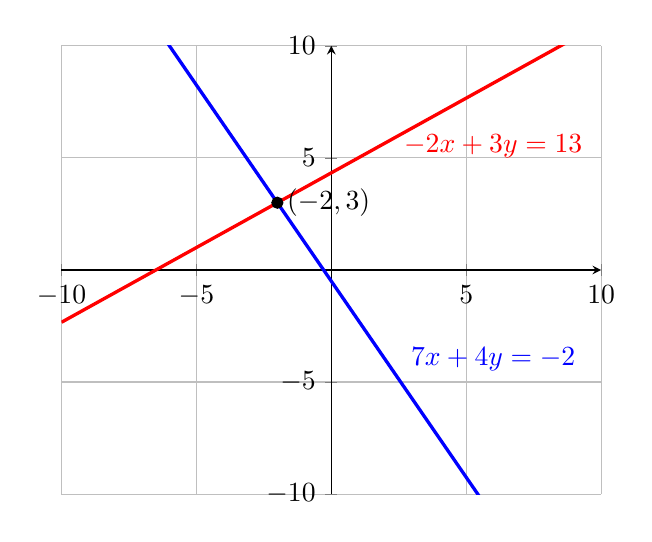
\begin{tikzpicture}
            \begin{axis}[
                axis lines=middle,
                grid=both,
                grid,
                ymin=-10,
                ymax=10,
                xmin=-10, 
                xmax=10
                ]       
                \addplot[mark=none, blue, very thick] coordinates {(-10,17) (10,-18)} node[above] at (axis cs:6,-5) {$7x+4y=-2$};
                \addplot[mark=none, red, very thick] coordinates {(-10,-2.3333) (10,11)} node[below] at (axis cs:6,6.5) {$-2x+3y=13$};
                \addplot[mark=*] coordinates {(-2,3)} node[right] at (axis cs:-2,3) {$(-2,3)$};
            \end{axis}
        \end{tikzpicture}
    \end{center}

    这种可视化方法也适用于三个方程和三个未知数的方程组,但这需要在三维空间中绘制图线。这在实践中可能很难做到,但在技术上是可行的。同样的概念也适用于多个方程和多个未知数,但在四维或更高维上画``线''对我们人类来说是可能是无法想象的!
\end{method}

\begin{method}{多于两个变量:消元!}
    该方法的下一部分建立在第一部分的基础上,通过不断应用第一部分的方法,将两个以上方程(和未知数)的方程组简化为更小的方程组,最终得到两个方程和两个未知数的方程组。我们通过一个三个方程和三个未知数的方程组来说明该方法,如下所示:
    $$
    \begin{cases}
        \enspace\: 6x - 3y + \enspace z = -1 \\
        -3x + 4y - 2z = 12 \\
        \enspace\: 5x + \enspace y + 8z = 6
    \end{cases}
    $$
    第一个目标是消除三个变量中的一个。本质上,这可以通过两种方式之一来完成,就像两个方程和两个未知数的方法一样。假设我们要从方程组中消除 $z$;我们可以尝试以某种方式用 $x$ 和 $y$ 来表示 $z$ 并代入,或者我们可以将某些方程乘以系数并相加,从而消除 $z$。这里唯一的区别是,无论我们选择哪种方法,我们都需要执行两次。我们用第一个方程得到
    \[z = -6x + 3y - 1\]
    将 $z$ 的表达式代入第二个和第三个方程后,我们将得到一个由两个方程和两个未知数组成的方程组。

    思考这个问题的一种方法是,我们需要来自所有三个方程的信息才能最终得出答案,因此在将方程组简化为两个方程时,我们需要以某种方式保留来自所有三个原始方程的信息。$z$ 的表达式来自第一个方程,因此我们需要将其代入其他两个方程以保留我们需要的所有信息。

    将其与以下步骤序列进行比较:整理第一个方程以分离 $z$ 并将其代入第二个方程,然后整理第二个方程式以分离 $z$,将其代入第一个方程。会发生什么?直觉告诉我们,在某种程度上``丢失''了第三个方程的信息,没错,我们将获得一个由两个方程和两个未知数组成的方程组,但它没有足够的信息得到 $x$ 和 $y$ 的唯一解。如果你真的执行了我们刚才描述的步骤(试着这样做来检查我们的工作),化简到最简后,可以得到以下两个方程的``方程组'':
    $$
    \begin{cases}
        9x - 2y = 10 \\
        \frac{9}{2}x - \:y = 5
    \end{cases}
    $$
    这两个方程其实是同一个方程!因此,我们实际上无法求解 $x$ 和 $y$ 的唯一值。

    让我们回到原来的位置,将上面 $z$ 的表达式代入第二和第三个方程
    \begin{align*}
        -3x + 4y - 2 \cdot (-6x + 3y - 1) &= 12 \\
        5x + y + 8 \cdot (-6x + 3y - 1) &= 6
    \end{align*}
    然后化简
    \begin{align*}
        9x - 2y &= 10 \\
        -43x + 25y &= 14
    \end{align*}
    应用第一个问题中的方法之一将解出 $(x, y) = (2, 4)$。有了这两个值,我们就可以代入三个原始方程中的任意一个并求出 $z$;更好的做法是,我们可以使用从第一个方程中得到的 $z$ 的表达式:
    \[z = -6x + 3y - 1 = -6 \cdot (2) + 3 \cdot 4 = 1 = -12 + 12 - 1 = -1\]
\end{method}

\begin{method}{多于两个变量:另一种消元方法!}
    将方程组从三个方程简化为两个方程的另一种方法与前面的``乘加''法有关。使用上面具有三个方程的方程组,我们可能会注意到,第一个方程乘以 $8$,第二个方程乘以 $4$ 后,所有三个方程中 $z$ 的系数都是 $\pm 8$。这使我们能够以简便的方式对方程进行加/减,将方程组简化为两个方程和两个未知数。具体来说,让我们做一遍刚才提到的操作
    \begin{align*}
        48x - 24y + 8z &= -8 \\
        -12x + 16y - 8z &= 48 \\
        5x + y + 8z &= 6
    \end{align*}
    然后将第一个方程与第二个方程相加
    \begin{align*}
        (48x - 12x) + (-24y + 16y) + (8z - 8z) &= -8 + 48 \\
        36x - 8y &= 40
    \end{align*}
    接着将第二个方程与第三个方程相加
    \begin{align*}
        (-12x + 5x) + (16y + y) + (-8z + 8z) &= 48 + 6 \\
        -7x + 17y &= 54
    \end{align*}
    上面操作将产生了两个仅包含 $x$和 $y$ 的方程;此外,我们结合了所有三个原始方程的信息来生成这些方程,所以我们可以确信我们没有``丢失''任何东西。用我们之前讨论的任意一种方法解此新方程组
    $$
    \begin{cases}
        \: 36x - \enspace 8y = 40 \\
        -7x + 17y = 54  
    \end{cases}
    $$
    都会解得 $(x, y) = (2, 4)$。将 $x$ 和 $y$ 的值代入三个原始方程中的任意一个并求出 $z$,即可得到我们要求的最终答案。

    我们也可以执行类似的步骤,从方程组中消除 $y$;例如,我们可以将第一个方程乘以 $4$ 与第二个方程乘以 $3$ 相加,然后用第二个方程减去第三个方程乘以 $4$。这些方法中的任何一种都会得到相同的最终答案,只是其中一些可能会缩短算术步骤或带来``更好计算''的数字(即更少的分数,更小的乘法,等等)。求解具有更多方程的方程组的一般过程:将方程相乘并相加,从方程组中消除一个变量,然后继续这样做,直到只有两个方程和两个未知数;然后,求解这两个变量的值,并反向代入运算,用这些值来求解已消除变量的值。
\end{method}

\subsubsection*{代数练习}

\begin{problem}
    求解关于 $(x, y, z)$ 的以下方程组:

    $$
    \begin{cases}
        \enspace x+y+z=15\\
        2x-y+z=8\\
        x-2y-z=-2
    \end{cases}
    $$

    求解关于 $(x, y, z)$ 的类似方程组:

    $$
    \begin{cases}
        \enspace x+y+z=15\\
        2x-y+z=9\\
        x-2y-z=-2
    \end{cases}
    $$

    比较两个方程组之间 $x$、$y$ 和 $z$ 值的变化。

    哪个变量变化最大?哪个最少?这些变化的比例是多少?

    通过改变方程组第二个方程右侧的常数,你可以使这个比率变多大/多小?
\end{problem}

\begin{problem}
    父亲、母亲和儿子坐在餐厅里吃饭,这时另一个由父亲、母亲和儿子组成的家庭走过来。第二个家庭惊讶于他们与第一个家庭如此相似,于是就问第一个家庭:``你们三个多大了?我猜我们的年龄都差不多''。第一个家庭的父亲恰好是一位数学家,不愿意轻易泄露家人的年龄,于是用一种巧妙的方式``透露''给其他人。他说:``我们现在的年龄加起来是 $72$ 岁,而我恰好是我儿子的六倍。然而,将来当我只是他年龄的两倍时,我们的年龄加起来将是我们现在年龄加起来的两倍。你猜我们多少岁?''\\
    三个家庭成员的年龄有多大?
\end{problem}

% !TeX root = ../../../book.tex
\subsection{多项式}

有时我们需要使用平方、立方或更高次幂的变量。一般来说,多项式是我们用于表示一个函数的术语,该函数具有一个或多个整数次幂的变量,乘以系数,然后相加。以下是多项式的一些例子:
\[x^2 - 7x + 1,\quad 7p^6 + 5p^4 + 3p^2 + 2p,\quad \frac{1}{2}z^2 + 9y^2z - 2y + z^3y^2 - 7z\]

这些类型的函数在数学中非常常见和流行,部分原因是它们具有方便的属性,另一部分原因是它们在自然界中的普遍存在。我们将在本书中频繁地看到它们。不过,现在让我们将目光聚焦在只有一个\emph{输入变量}的多项式。

\subsubsection*{多项式的根}

有时,我们会在谜题中定义一个多项式函数,并想知道输入变量是否有任何值可以使输出值为 0。这些让输出值为 0 的输入值称为多项式的\textbf{根}。

识别多项式根的一种方法是将其隐式\textbf{因式分解}为线性项;也就是说,我们尝试将函数表示为一系列乘法而不是加法,因为我们可以声明(至少)其中一个因子为 $0$ 输出值才 $0$。该技术背后的动机依赖于以下事实:

\begin{quote}
    \textbf{事实:}如果 $a$ 和 $b$ 为实数且 $ab=0$,则 $a=0$ 或 $b=0$(或者两者都等于零)。
\end{quote}

\begin{example}
    我们来看一个具体的例子。尝试分解以下多项式:
    \[p(x) = x^2 + 6x + 8\]
    (将多项式定义为 $p(x)$ 是常见的表示法,其中 $p$ 代表多项式,$x$ 是输入变量,$p(x)$ 是与输入值 $x$ 对应的输出值。)

    你可能已经注意到
    \[p(x) = x^2 + 6x + 8 = (x + 4) \cdot (x + 2) = (x + 4)(x + 2)\]
    (当存在用括号分隔的因子时,删除 $\cdot$ 也是相当常见的,因此我们从现在开始也将采用该约定。)

    这种因式分解之所以有效,是因为我们多次相反地应用分配律。如果我们展开刚刚的因式分解,明确显示其中每一步,它看起来像:

    \begin{align*}
        p(x) &= (x + 4)(x + 2) \\
        &= x(x + 2) + 4(x + 2) \\
        &= (x^2 + 2x) + (4x + 8) \\
        &= x^2 + 2x + 4x + 8 = x^2 + 6x + 8
    \end{align*}

    我们真正写下因式分解步骤是为了注意到项 $+4$ 和 $+2$ 具有乘积 $+8$,这正是常数项,并且它们之和为 $+6$,而这正是 $x$ 项的系数。知道这些因式的后续展开如何进行,我们就可以在不进行检验的情况下写下因式分解。
\end{example}

\subsubsection*{二次因式分解}

让我们以上面示例为例,尝试推广到任何二次函数。如果我们想分解一个二次多项式
\[p(x) = x^2 + bx + c\]
我们要求 $r$ 和 $s$ 的值,使得 $r \cdot s = c$ 且 $r + s = b$。通常,我们可以``通过试算''来做到这一点,或者只需盯着这两个方程思考一分钟即可得出适当的值。(这就是我们在前一个例子中所做的!)

如果 $x^2$ 项的系数不是 $1$ 而是其他数字 $a$,该怎么办?请注意,如果我们可以对多项式 $\frac{p(x)}{a} = x^2+\frac(b)(a)x+\frac{c}{a}$ 进行因式分解,那么我们也可以通过乘以 $a$ 来找到原始多项式 $p(x)$ 的因式分解。这不会影响我们求多项式根(我们最初的目标)的能力,因为我们假设 $a \ne 0$(否则我们一开始就没有二次多项式,也就无需分解它)。一旦我们找到了这个因式分解,就很容易确定 $p(x)$ 的根;因为我们想知道何时 $p(x) = 0$,所以我们可以使用因式分解和上面提到的事实来得出结论:
\begin{align*}
    0 = p(x) = (x + r)(x + s) & \quad \text{ 意味着 } x + r = 0 \text{ 或 } x + s = 0 \\
    & \quad \text{ 即 } x = -r \text{ 或 } x = -s
\end{align*}
也就是说,根为 $-r$ 和 $-s$。

如果我们有一个 $p(x) = x^2 - a^2$ 形式的多项式怎么办?这种特殊类型的函数称为\textbf{平方差},具有快速分解技巧。这是一个二次多项式,因此,按照上面的方法,我们要求 $r,s$ 的值,使得 $rs = -a^2$ 且 $r + s = 0$(因为 $p(x)$ 中没有 $x$ 项)。第二个条件告诉我们 $r = -s$,代入第一个条件可得 $r^2 = a^2$。 因此,令 $r = a$ 和 $s = -a$ 实现因式分解 $p(x) = (x - a)(x + a)$,因此根为 $\pm a$。(请注意,$r = -a$ 和 $s = a$ 也满足这两个条件,但实际上会产生相同的 $p(x)$ 因式分解。)

类似的技巧有时可以应用于更高\textbf{次}的多项式(回想一下,``次''意味着输入变量的最高次幂)。例如,以下多项式的次数为 4
\[p(x) = 4x^4 - x^2 - 3\]
如果我们定义 $y = x^2$ 并将其写成二次多项式,我们就可以轻松分解它
\[p(y) = 4y^2 - y - 3 = (4y + 3)(y - 1)\]
请注意,你可以考虑 $y^2$、$y$ 的系数和常数项的分解,从而直接跳转到我们上面的分解方法或除法技巧。这里,我们想要分解 $\frac{p(y)}{4} = y^2-\frac{1}{4}=\frac{3}{4}$,因此我们令 $rs = -\frac{3}{4}$ 和 $r + s =-\frac{1}{4}$; $r=-1, s=+\frac{3}{4}$ 满足,所以我们得到因式分解
\[\frac{p(x)}{4} = (y+(-1))\Big(y+\frac{3}{4}\Big)\]
化简得
\[p(x) = 4(y-1)\Big(y+\frac{3}{4}\Big) = (y-1)(4y+3)\]
这正是我们之前的方法。

\subsubsection*{一根一因子}

当然,这种识别根的技巧也可以反向发挥作用:如果我们可以轻松地找到多项式的根,这可以帮助我们识别其中一个因子。举个例子,请看下面的三次多项式,看看能否``通过试算''找到根;也就是说,看看能否找到 $x$ 的输入值,使 $p(x)$ 的计算结果为零:
\[p(x) = x^3 - 3x + 2\]
如果您还没有找到,你可以试着代入一些``简单值'',例如前几个整数(正数和负数),看看会发生什么。如果这样做,你会发现 $p(1) = 1 - 3 + 2 = 0$。因此,我们知道多项式 $p$ 的因式分解应包含因子 $(x - 1)$,因为它对应于根 $x = 1$。知道了这一点,我们就可以将 $p(x)$ 除以因子 $(x - 1)$,从而可以进一步对商进行因式分解并确定 $p$ 的所有根。

\subsubsection*{多项式``除法''}

那么我们要如何除多项式呢?我们要求另一个多项式 $q(x)$ 使得 $p(x) = q(x) \cdot (x - 1)$,或者换句话说,我们需要找到 $\frac{p(x)}{x-1}$。找到此类函数的一种方法是使用与你在中学学习整数除法时学到的\textbf{长除法}原理。相同的概念也适用于多项式函数!回想一下除法的工作原理,并尝试通过一些基本示例 --- 例如 $22 \div 7$ --- 来唤起你对除法工作原理的记忆。

现在,让我们尝试将同样的原理应用于多项式。这是将长除法的思想应用于 $\frac{x^3-3x+2}{x-1}$ 的示例:

\[
\arraycolsep=1pt
\begin{array}{*1r @{\hskip\arraycolsep}c@{\hskip\arraycolsep} *{9}r}
        &          &   &      &   & x^2 & + &  x & - & 2 &  \\
\cline{2-11}
x-1     & \longdiv &   & x^3  &   &  & -    & 3x & + & 2 &  \\
        &          & - & x^3  & + & x^2 &   &    &   &   &  \\
\cline{3-6}
        &          &   &      &   & x^2 & - & 3x &   &   &  \\
        &          &   &      & - & x^2 & + &  x &   &   &  \\
\cline{5-8}
        &          &   &      &   &     & - & 2x & + & 2 &  \\
        &          &   &      &   &     &   & 2x & - & 2 &  \\
\cline{7-11}
        &          &   &      &   &     &   &    &   & 0 &  \\
\end{array}
\]

在该方法的每次迭代中,我们尝试找到可以``得到''更高次幂的最大``因子''。在这种情况下,这些因子只是乘以 $x$ 的幂;我们确定可以``得到''当前相关项的 $x$ 的最大幂。由于被除数为 $x^3$,除数为 $x$,因此我们在除法线上方写上 $x^2$。然后,我们将 $(x-1)$ 乘以 $x^2$,将其写在被除数下方,然后相减求出余数。

重复相同的过程,直到除法线上方出现常数项(即 $x^0$ 的倍数)并查看余数。由于这里的余数为 $0$,所以我们知道我们得到了一个没有余数的因式分解。然后,我们注意到 $r=2, s=-1$ 满足 $r+s=1$ 且 $rs=-2$,因此结果二次多项式可以进一步分解,最终得到
\[p(x) = (x - 1)(x - 1)(x + 2) = (x - 1)^2(x + 2)\]

多项式的次数为 $3$,但函数只有 $2$ 个根。这是否让你感到奇怪?你能想到一个只有 $1$ 个根的 $3$ 次多项式吗?没有根的 $3$ 次多项式会是怎样?拥有 $4$ 个根、$5$ 个根或更多根呢?这有可能吗?为什么可能或为什么不可能?如果是 $4$ 次多项式会怎样?$n$ 次呢?你能确定多项式根的数量与其次数的关系吗?

\subsubsection*{因式展开}

有时,在解决难题时,我们会从多项式的因式分解开始,并希望完全扩展因子,以便我们可以确定特定项的系数。我们如何快速、轻松地将多项式相乘?本质上,我们一遍又一遍地应用分配律,而不必写出所有步骤(尽管这种基本的、一步一步的程序保证有效,所以如果你不确定你的答案是否正确,最好回去彻底检查每一步)。

有种特殊的情况可以减少所涉及的步骤,那就是当我们需要展开像 $(a+b)^n$ (其中 $a$ 和 $b$ 代表任意常量或变量,$n$ 为整数)这样的因式分解时。在这种特定情况下,有一种方便的方法来确定展开多项式的系数,这些值来自\textbf{帕斯卡三角}。

这是一种将整数行排列成三角形的排列,其中每行对应于这种展开中 $n$ 的特定值。生成帕斯卡三角形的诀窍是先将前两行全写为 $1$,再将三角形的外侧``边''全写为 $1$。在三角形的内部,任何条目都可以通过将该条目左上方和右上方的两个条目相加得到。试着自己生成三角的前几行,并与下面的三角进行比较,以确保你正确完成了该过程。

\begin{center}
    \begin{tabular}{rccccccccc}
        $n=0$: &    &    &    &    &  1\\\noalign{\smallskip\smallskip}
        $n=1$: &    &    &    &  1 &    &  1\\\noalign{\smallskip\smallskip}
        $n=2$: &    &    &  1 &    &  2 &    &  1\\\noalign{\smallskip\smallskip}
        $n=3$: &    &  1 &    &  3 &    &  3 &    &  1\\\noalign{\smallskip\smallskip}
        $n=4$: &  1 &    &  4 &    &  6 &    &  4 &    &  1\\\noalign{\smallskip\smallskip}
    \end{tabular}
\end{center}

我们将 $n$ 值写在左侧,表示与展开 $(a+b)^n$ 的对应关系。一般来说,展开式的任何项都是某个系数(取自帕斯卡三角)乘以 $a^kb^{n-k}$,其中 $k$ 的值介于 $0$ 到 $n$ 之间。也就是说,展开式每一项种,$a$ 和 $b$ 的幂之和必须为 $n$。三角形任何一行中的数字都是按照 $a$ 的幂降序书写的,所以第一个 $1$ 是 $a^n$ 的系数,下一个数字是 $a^{n-1}b$ 的系数,依此类推。

如果我们要展开 $(a + b)^2$,我们会读取帕斯卡三角的 $n = 2$ 行,得到系数为 $1, 2, 1$,这些系数分别是 $a^2, ab, b^2$ 的系数。因此,
\[(a + b)^2 = a^2 + 2ab + b^2\]
我们也可以轻松地手动完成展开。但如果我们要展开 $(x^2+2)^4$ 怎么办?这不是手动能快速完成的,所以让我们试试使用帕斯卡三角会发生什么。$n = 4$ 行告诉我们 $a^4, a^3b, a^2b^2, ab^3, b^4$ 的系数分别为 $1, 4, 6, 4, 1$,其中 $a = x^2, b = 2$。因此,我们可以写成
\begin{align*}
    (x^2+2)^4 &=  1 \cdot (x^2)^4 + 4 \cdot (x^2)^3 \cdot 2 + 6 \cdot (x^2)^2 \cdot (2)^2 + 4 \cdot x^2 \cdot (2)^3 + 1 \cdot (2)^4 \\
    &=  x^8 + 4 \cdot x^6 \cdot 2 + 6 \cdot x^4 \cdot 4 + 4 \cdot x^2 \cdot 8 + 16 \\
    &= x^8 + 8x^6 + 24x^4 + 32x^2 + 16
\end{align*}
尝试逐步执行此展开并进行比较。实际上,帕斯卡三角有一些非常有趣的性质,这些性质深深植根于其他一些数学概念中,这些性质在\textbf{组合数学}领域特别有用。事实上,我们稍后将更详细地研究其中许多性质!例如,你可能想知道为什么这个过程 --- 添加上面的两个条目 --- 会生成与这样的展开因子相对应的条目。当我们讨论\textbf{二项式定理}及其相关思想时,我们将证明它的有效性!(如果您感到好奇,请参阅 \ref{sec:section8.4.4} 节。)

\subsubsection*{配方}

在得出重要结果之前,我们还需要提及一个与多项式相关的技巧。有时,将多项式重写为平方项加常数项是非常有用的,这样我们就可以以方便的方式分离变量和常数。这相当于添加再减去一个特定项,因此,总的来说,我们在多项式中添加了 $0$,但选择该项的方式可以让我们方便地重写多项式的项。这个过程被称为\textbf{配方},即我们添加一项来创建平方因子,并通过减去相应的量来保持多项式不变。

让我们通过一个例子来说明这个过程,然后再尝试进行概括。请看下面的多项式:
\[p(x) = x^2 + 8x + 9\]
因式分解在这里并不明显,所以让我们尝试配方。我们想要得到类似 $(x + a)^2$ 这样的项,其中我们知道 $x$ 的系数为 $1$,因为多项式种有 $1 \cdot x^2$。将其展开得 $x^2+2ax+a^2$。由于我们需要得到 $8x$,所以我们应该令 $a = 4$。因此展开得到 $x^2 + 8x + 16$,但原式的常数项为 $+9$,所以我们向原多项式中加上 $7$ 再减去 $7$: 
\[p(x) = x^2 + 8x + 9 + 7 - 7 = (x^2 + 8x + 16) - 7 = (x + 4)^2 - 7\]
上面的式子看起来眼熟吗?准确地说,它是平方差,我们知道如何分解它:
\begin{align*}
    p(x) &= x^2 + 8x + 9 = (x + 4)^2 - 7 = (x + 4)^2 - \Big(\sqrt 7\Big)^2 \\
    &= \Big(x+4+\sqrt 7\Big)\Big(x+4-\sqrt 7\Big)
\end{align*}
因此,该多项式的根为 $x=-4-\sqrt 7$ 和 $x=-4+\sqrt 7$。

让我们来泛化一下!假设我们从以下形式的二次多项式开始
\[p(x) = ax^2 + bx + c\]
为了能够配方,我们需要添加再减去一个特定项。我们之前是如何找到这个项的?像 $(rx + s)^2$ 这样的项展开后得 $r^2x^2 + 2rsx + s^2$,并且为了将这些系数与原多项式的系数相匹配,我们发现需要让 $r^2 = a$,所以我们需要令 $r = \sqrt{a}$。(注意,这里要求 $a \ge 0$!如果 $a<0$ 该怎么办?)然后,为了让 $2rs = b$,我们需要令 $s = \frac{b}{2r} = \frac{b}{2\sqrt{a}}$,接着,当它展开时,我们添加 $s^2 = \frac{b^2}{4a}$,再从多项式中减去。

下面公式执行了上述步骤,并进行一些额外的代数整理,让项``更好看'':
\begin{align*}
    p(x) &= ax^2 + bx + c = ax^2 + bx + \frac{b^2}{4a} + c - \frac{b^2}{4a}\\
    &=\Big(\sqrt{a}x+\frac{b}{2\sqrt{a}}\Big)^2+\Big(c- \frac{b^2}{4a}\Big)\\
    &=\Big(\sqrt{a}\Big(x+\frac{b}{2a}\Big)\Big)^2+\Big(c- \frac{b^2}{4a}\Big)\\
    &=a\Big(x+\frac{b}{2a}\Big)^2+\Big(c- \frac{b^2}{4a}\Big)
\end{align*}
现在,我们知道了如何对给定的任何二次多项式进行配方!

\subsubsection*{可视化配方}

有一个记住如何执行上述配方过程的有效方法。它基于正方形和矩形面积的可视化表示。

假设 $a, b>0$,这样我们就可以从几何角度将 $ax^2+bx$ 解释为矩形的面积。具体来说,我们将 $ax^2$ 项视为正方形的面积。这意味着正方形的边长为 $\sqrt{a} \cdot x$: 

\begin{center}
    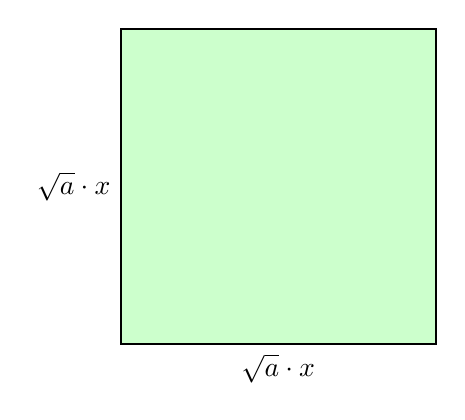
\begin{tikzpicture}[thick, scale=1]
        \fill [color=green,opacity=0.2] (0,0) rectangle +(4,4);
        \draw (0,0) rectangle +(4,4);
        \path (0,0) -- (4,0) node[midway,below] {$\sqrt{a}\cdot x$};
        \path (0,0) -- (0,4) node[midway,left] {$\sqrt{a}\cdot x$};
    \end{tikzpicture}
\end{center}

那么我们应该如何表示 $bx$ 这一项呢?我们要把正方形扩展到更大的正方形;这就是配方的意义。因此,我们需要围绕正方形构建一些矩形,这将有助于我们实现这一目标。让我们将 $bx$ 项代表的面积分成两个矩形,每个矩形的面积为 $\frac{b}{2}x$。由于矩形必须有一条边的长度为 $\sqrt{a} \cdot x$,并且我们希望矩形面积为 $\frac{b}{2}x$,因此另一条边长必然为 $\frac{b}{2\sqrt{a}}$: 

\begin{center}
    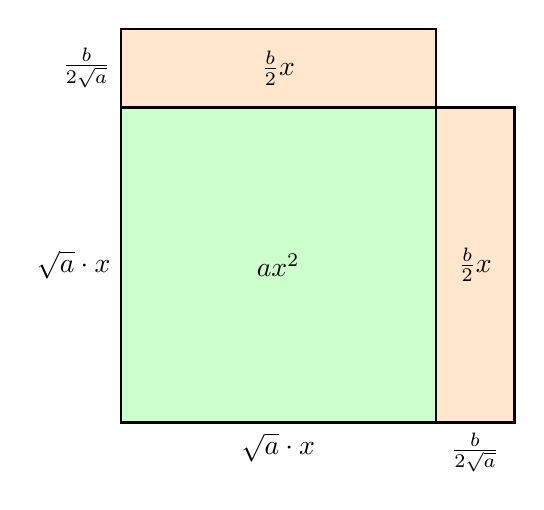
\begin{tikzpicture}[thick, scale=1]
        \fill [color=green,opacity=0.2] (0,0) rectangle +(4,4);
        \draw (0,0) rectangle +(4,4) node[pos=.5, align=center]{$ax^2$};
        \path (0,0) -- (4,0) node[midway,below] {$\sqrt{a}\cdot x$};
        \path (0,0) -- (0,4) node[midway,left] {$\sqrt{a}\cdot x$};

        \fill [color=orange,opacity=0.2] (4,0) rectangle +(1,4);
        \draw (4,0) rectangle +(1,4) node[pos=.5, align=center]{$\frac{b}{2}x$};
        \path (4,0) -- (5,0) node[midway,below] {$\frac{b}{2\sqrt{a}}$};

        \fill [color=orange,opacity=0.2] (0,4) rectangle +(4,1);
        \draw (0,4) rectangle +(4,1) node[pos=.5, align=center]{$\frac{b}{2}x$};
        \path (0,4) -- (0,5) node[midway,left] {$\frac{b}{2\sqrt{a}}$};
    \end{tikzpicture}
\end{center}

我们需要添加什么才能使上面的图形变成为一个正方形?我们发现只需在右上角填充一个小正方形即可。小正方形边长为 $\frac{b}{2\sqrt{a}}$,因此它的面积 --- 我们需要添加的项--- 为 $\frac{b^2}{4a}$。

\begin{center}
    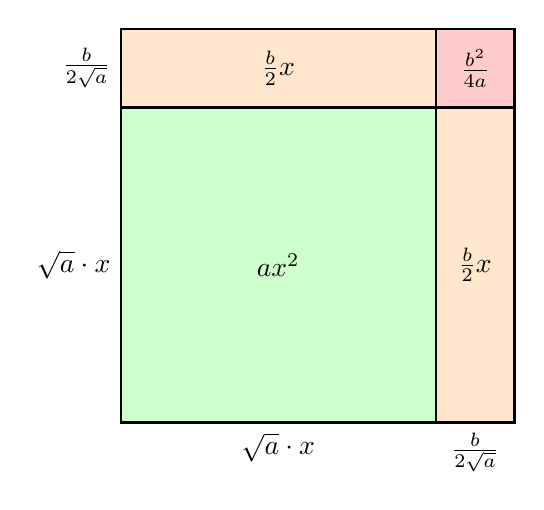
\begin{tikzpicture}[thick, scale=1]
        \fill [color=green,opacity=0.2] (0,0) rectangle +(4,4);
        \draw (0,0) rectangle +(4,4) node[pos=.5, align=center]{$ax^2$};
        \path (0,0) -- (4,0) node[midway,below] {$\sqrt{a}\cdot x$};
        \path (0,0) -- (0,4) node[midway,left] {$\sqrt{a}\cdot x$};

        \fill [color=orange,opacity=0.2] (4,0) rectangle +(1,4);
        \draw (4,0) rectangle +(1,4) node[pos=.5, align=center]{$\frac{b}{2}x$};
        \path (4,0) -- (5,0) node[midway,below] {$\frac{b}{2\sqrt{a}}$};

        \fill [color=orange,opacity=0.2] (0,4) rectangle +(4,1);
        \draw (0,4) rectangle +(4,1) node[pos=.5, align=center]{$\frac{b}{2}x$};
        \path (0,4) -- (0,5) node[midway,left] {$\frac{b}{2\sqrt{a}}$};

        \fill [color=red,opacity=0.2] (4,4) rectangle +(1,1);
        \draw (4,4) rectangle +(1,1) node[pos=.5, align=center]{$\frac{b^2}{4a}$};
    \end{tikzpicture}
\end{center}

看呐!这与我们上面通过代数推导得出的项完全相同。通过添加它,我们可以将这些项分解为完全平方。只需要再将其也减去,以确保原表达式不变。

这是一个需要记住的有用技巧。它可以提醒你配方的过程动机以及如何实现它。不过,你应该思考一件事:为什么这种可视化表示有效?我们必须假设 $a, b > 0$ 才能画出这些图,那么为什么无论 $a$ 和 $b$ 是什么,通向公式都有效呢?

\subsubsection*{二次函数求根公式}

让我们回到求多项式的根的问题。具体来说,让我们回忆一下\textbf{二次函数求根公式}。你可能已经记住这个公式是``求解二次方程''的一种方法,但你知道它为什么有效吗?让我们试着弄清楚吧!一般来说,我们从以下形式的二次多项式开始
\[p(x) = ax^2 + bx + c\]
其中 $a \ne 0$(否则,它就不是二次多项式),并且我们想要求 $p(x) = 0$ 时 $x$ 的值。(你是否尝试过回答我们上面提出的关于此类多项式有几个根的问题?在以下推导过程中请记住这些概念。)将该多项式因式分解为线性因子很麻烦,所以我们使用上面介绍的方法:配方。该方法的好处是,我们可以设置 $p(x)=0$,并在配方后重新整理项来求解 $x$。观察:
\[0 = p(x) = ax^2 + bx + c =a\Big(x+\frac{b}{2a}\Big)^2+\Big(c- \frac{b^2}{4a}\Big)\]
化简可得
\[\frac{b^2}{4a} -c = a\Big(x+\frac{b}{2a}\Big)^2\]

现在,我们要开始``撤消''此处的配方来求解 $x$,这需要对两边求平方根。但如果 $\frac{b^2}{4a} -c < 0$ 呢?我们根本无法求平方根!如果 $\frac{b^2}{4a} -c = 0$ 呢?会有问题吗?当 $\frac{b^2}{4a} -c > 0$ 时会有什么问题吗?这些问题与我们之前关于多项式可能有的根数相关。你可能已经(正确地)推断出二次多项式最多可以有两个根,但在这里我们发现二次多项式可能有一个或零个根(及其原因)!

\begin{itemize}
    \item 当 $\frac{b^2}{4a} -c < 0$ 时,那么 $x$ 的任何值都\emph{不}可能满足上面推导中的最后一行公式。因此,$p(x)$ 无实数根。
    \item 当 $\frac{b^2}{4a} -c = 0$ 时,那么对上面最后一行公式两边取平方根是完全有效的,但只会产生\emph{唯一一个 }$x$ 值:
    \begin{align*}
        \frac{b^2}{4a} -c = 0 &= a\Big(x+\frac{b}{2a}\Big)^2 \\
        0 &= x+\frac{b}{2a} \\
        x &= -\frac{b}{2a}
    \end{align*}
    \item 当 $\frac{b^2}{4a} -c > 0$ 时,此时,我们预期 $p(x)$ 有\emph{两个}根,因为两边取平方根会引入两个可能的解。一般来说,当我们遇到像 $s^2 = t$ 这种情况时,我们可以说唯一可能的解是 $s =\sqrt{t}$ 和 $s = -\sqrt{t}$,但我们必须同时考虑两者(通常将其写做 $s = \pm\sqrt{t}$)。在这种情况下求解 $x$ 得
    \begin{align*}
        \frac{b^2}{4a} -c &= a\Big(x+\frac{b}{2a}\Big)^2 \\
        \pm\sqrt{\frac{b^2-4ac}{4a}} &= \sqrt{a}\Big(x+\frac{b}{2a}\Big) = \sqrt{a}x+\frac{b}{2\sqrt{a}} \\
        -\frac{b}{2\sqrt{a}}\pm\frac{\sqrt{b^2-4ac}}{\sqrt{4a}} &= \sqrt{a}x \\
        -\frac{b}{2a}\pm\frac{\sqrt{b^2-4ac}}{\sqrt{4a^2}} &= x
    \end{align*}
    现在,我们必须小心对待之前进行的平方根观察。一般来说,$\sqrt{4a^2} = \pm2a$,但我们知道分子上的平方根项已经有一个相关的 $\pm1$ 因子,因此分母上的因子不会改变这一点。因此,我们可以得出结论
    \[x = -\frac{b}{2a}\pm\frac{\sqrt{b^2-4ac}}{2a} = \frac{-b\pm\sqrt{b^2-4ac}}{2a}\]
    这就是二次函数求根公式!
\end{itemize}

请记住,推导的最后一种情况是在 $\frac{b^2}{4a} -c > 0$ 的假设下进行的。当 $\frac{b^2}{4a} -c = 0$ 时,该公式依然适用吗?在这种假设下,我们是否可以执行与上面相同的步骤?为什么可以或者为什么不可以?

\subsubsection*{问题}

\begin{problem}
    找出 $a$ 的所有可能值,使 $x-a$ 是 $x^2+2ax-3$ 的因子。
\end{problem}
\begin{problem}
    找出 $b$ 的所有可能值,使得 $x^3 + b$ 可以被 $x + b$ 整除,没有余数。
\end{problem}
\begin{problem}
    对于任意自然数 $n$,因子 $x^n - 1$。
\end{problem}
\begin{problem}
    确定如下公式定义的 $x$ 的值
    \[x = \sqrt{2+\sqrt{2+\sqrt{2+\sqrt{2+\dots}}}}\]
    \begin{hint}
        尝试用 $x$ 本身来表示无限嵌套的平方根。
    \end{hint}
\end{problem}
\begin{problem}
    用配方法证明正数 $n$ 及其倒数之和始终大于或等于 $2$,并且唯一使和等于 $2$ 的数字是 $n = 1$。
    \begin{hint}
        求和,加减 $2$,然后重新整理。
    \end{hint}
\end{problem}
\begin{problem}
    如何求 $ax^4 + bx^2 + c$ 形式的四次多项式的根?
\end{problem}

% !TeX root = ../../../book.tex
\subsection{集合漫谈}

我们已经提到了一些特定类型的数字,但我们想具体定义我们将来要使用的数字集。这些数字集合都由一个特定字母用黑板粗体表示。\textbf{自然数}(也称为整体数(whole numbers)或计数数(counting numbers))之所以被称为自然数,是因为当我们计数物体时,用自然数感觉很``自然''。自然数可以写做
\[\mathbb{N} = \{1, 2, 3, 4, 5, \dots\}\]
(自然数有一个更具体更技术性的定义,我们将在稍后解释。)\\
我们用 $\mathbb{N}$ 表示 ``自然(natural)''

使用 $\mathbb{N}$,我们可以定义一个相关的数字集合:所有\textbf{整数}的集合,它包含了自然数、$0$ 和负自然数。整数可以写做
\[\mathbb{Z} = \{\dots, -3, -2, -1, 0, 1, 2, 3, \dots\}\]
字母 $\mathbb{Z}$ 来自德语单词 \emph{Zahlen},意思是``数字''。

从整数集合,我们可以定义\textbf{有理数}的集合。这些数字可以表示为整数的比率,但它们似乎没有像集合 $\mathbb{N}$ 和 $\mathbb{Z}$ 那样自然的``列表'',所以我们不能像上面那样书写这个集合。为此,我们使用一个非常常见的集合表示法,如下所示:
\[\mathbb{Q} = \Big\{\frac{a}{b} \mid a,b \in \mathbb{Z} \text{ 且 } b \ne 0\Big\}\]
读作:
\begin{quote}
    ``有理数集是所有 $\frac{a}{b}$ 形式的数的集合,其中 $a$ 和 $b$ 都是整数,且 $b$ 不为零。''
\end{quote}
这表达了有理数是分数的必要信息,其中分子和分母都是整数(但分母不能为 $0$,因为除以 $0$ 是不允许的)。我们使用字母 $\mathbb{Q}$ 表示有理数,是因为 $\mathbb{R}$ 已经被用于表示实数,而 $\mathbb{Q}$ 是上一个可用的字母。此外,$\mathbb{Q}$ 包含所有整数的商,所以这也是有道理的!

\textbf{实数} $\mathbb{R}$ 有一个非常技术性的定义,遗憾的是,我们无法在本书中全面深入研究。(这恰恰表明,从数学上定义这个集合是多么困难!) 目前,思考实数的一种方法是通过\textbf{数轴}。实数是数轴上所有的数字,而 $\mathbb{N}$、$\mathbb{Z}$ 和 $\mathbb{Q}$ 中的数字是数轴上的特定数字,它们并不构成整条数轴。某种程度上,$\mathbb{R}$ 是 $\mathbb{Q}$ 的``补全'',即``填补有理数之间的空白''。


% !TeX root = ../../../book.tex
\subsection{符号加油站}\label{sec:section1.3.5}

一种流行且方便的求和与求积的写法是使用缩写符号,将多个项或因子写成一种通用的形式。例如,如果我们想谈论前 $500$ 个自然数之和,该怎么写呢?写出总和的全部 $500$ 项会很乏味,所以 $1+2+3+\dots+499+500$ 是更常见的写法。(事实上,我们已经使用过这样的省略号。 你明白我们的意思吗?)这种写法很流行,并且确实表达了观点,但一些数学家对中间多余的省略号感到不满。我们推迟到现在才讨论这个问题,是因为符号通常很难学习和理解。我们并没有立即用新符号轰炸你,而是诉诸我们对 ``$\dots$'' 作用的直观理解。

既然我们已经提出来了,让我们看看如何避免使用省略号。为了写出我们上面提到的求和,我们将使用以下符号:
\[1+2+3+\dots+499+500 = \sum_{i=1}^{500}i\]
大写西格玛 $\sum$ 来自对应英文字母 S 的希腊字母,代表``求和''。\textbf{索引} $i$ 告诉我们求和的各个项的值。在 $\sum$ 符号下面写 $i = 1$,在 $\sum$ 符号上面写 $500$ 意味着我们让 $i$ 表示 $1$ 到 $500$(含)之间的所有自然数值。我们将这些值代入求和项的通用表达式,在本例中就是 $i$。因此,根据要求,求和项为 $1,2,3,\dots,500$。通过改变求和项表达式和/或索引的值,试着找到一些其他的写法。如果我们想求前 $500$ 个偶自然数之和怎么办?想求 $500$ 以内(含)所有偶自然数又该怎么办呢?尝试用上面的符号样式写出这些求和。

与此相关的是 $\prod$ 表示法。如果我们想查看前 $500$ 个自然数的乘积,我们将遵循相同的约定来识别索引值和通项:
\[1+2+3+\dots+499+500 = \prod_{i=1}^{500}i\]
大写派 $\prod$ 来自对应英文字母 P 的希腊字母,代表``求积''。再次尝试通过更改求积项和/或索引值以不同的方式表达上面公式。如果我们想求前 $500$ 个偶自然数的乘积怎么办?想求 $500$ 以内(含)所有偶自然数之积又该怎么办呢?尝试用上面的符号样式写出这些求积。

\subsubsection*{问题}

\begin{problem}
    用自然语言来描述以下等式的含义:
    \[\sum_{i=1}^{n}i^2 = \frac{n(n+1)(2n+1)}{6}\]
\end{problem}
\begin{problem}
    用适当的符号表达 $2$ 的前 $n$ 次幂的和与积,从 $2^0=1$ 开始。你能证明这个求和和求积公式吗?
\end{problem}
\begin{problem}
    考虑 $17$ 到 $33$(含)之间的所有奇数之和。索引 $0$ 开始,用求和符号写出这个求和公式。现在试着将索引从 $1$ 开始,重写求和公式。现在试着将索引从 $8$ 开始,重写求和公式,然后将索引从 $9$ 开始。以下哪一个感觉``更自然''?为什么?
\end{problem}

\newpage
% !TeX root = ../../../book.tex
\section{智力谜题}\label{sec:section1.4}

让我们把迄今为止讨论过的一些原则付诸实践。具体来说,让我们研究一些有趣的数学难题并解释如何解决它们。这些问题都不涉及除基本代数和算术之外的知识,但这并不意味着它们``基础''或``简单'',因为解决并理解这些问题都涉及批判性思维技能和敏锐的洞察力。在此过程中,我们将运用我们已经提出的一些逻辑思想。我们可能需要用到多项式函数,或者用代数方法求解一些方程。我们可能需要仔细考虑论证的顺序和流程,确保一切都遵循前面的知识或推论。总的来说,我们还应该思考什么构成了我们发现事实的良好且有效的\emph{证明}!

% !TeX root = ../../../book.tex
\subsection{消失的钞票}

\subsubsection*{问题描述}

这个经典的谜题包含在一个关于分摊酒店房间费用的故事中:

\begin{quote}
    三个朋友自驾旅行,深夜入住酒店。值班店员说当晚只剩一间空房,三人合住需付 $30$ 美元。他们疲惫不堪,便同意合住,每人各付 $10$ 美元预付款。店员道谢后递过钥匙,三人随即去车上取行李。此时,前来换班的另一名店员发现前一名店员多收了房费:实际只需 $25$ 美元。于是他从收银机取出一张 $5$ 美元钞票,递给值班服务生说:``把钱退给 29 号房的客人,我们多收费了。''服务生点头后走向三人房间。客人开门时对退款又惊又喜。为公平起见,一人将钞票换成五张 $1$ 美元纸币,每人取回 $1$ 美元,剩余 $2$ 美元作为小费给了服务生。服务生道谢后离开。

    现在,三人每人实际支付 $9$ 美元房费,加上 $2$ 美元小费,总计 $29$ 美元。但他们最初支付了 $30$ 美元……消失的 $1$ 美元去哪儿了?!
\end{quote}

请仔细思考一下,然后再翻页阅读解答。

\clearpage

\subsubsection*{解答:追踪资金流向}

你搞明白了吗?其实没有任何东西凭空``消失''。这个谜题的目的就是迷惑读者,误导他们去寻找不存在的事物。题目中的数字经过精心设计,使``消失的金额''仅为 $1$ 美元,让读者误以为发生了什么神秘事件。但通过细致的逻辑分析,你会发现最终提问本身并不合理:它利用了读者对情境的误解,使其忽视逻辑推理。若数字差异变得更大,人们便不会执着于寻找``消失的钞票''。

首先,让我们分析一下在这个特殊案例中到底发生了什么。关键在于厘清资金的实际流向。我们可将参与者分为两组:朋友群体(记为 $F$)和酒店员工群体(包括店员与服务生,记为 $H$)。现在,让我们重现资金转移步骤:

\begin{enumerate}
    \item $F$ 支付 $H \quad 30$ 美元(原始房费)
    \item $H$ 退还 $F \quad \enspace 5$ 美元(多收房费退款)
    \item $F$ 支付 $H \quad \enspace 2$ 美元(服务生小费)
    \item 净变化:$F$ 向 $H$ 支付 $30 \text{\ 美元} -5 \text{\ 美元} + 2 \text{\ 美元} = 27 \text{\ 美元}$
\end{enumerate}

这样就清晰了:退款 $5$ 美元使实际房费变为 $25$ 美元,三人每人付了 $9$ 美元,再加上服务生的小费,共计 $27$ 美元。谜题错误地将小费与房费相加,但 $27$ 美元已包含全部支出。通过追踪群体间的资金流动,我们能准确还原交易过程。

\subsubsection*{泛化:改变数字}

让我们应用上述方法来修改问题,通过改变数字消除对``消失的钞票''的情感依赖,同时放大金额差异。首先定义变量表示各步骤的金额。与其``测试''特定数值,不如引入变量实现``一次性全面验证''。

设 $3n$ 表示三人首次支付的房费总额($n$ 为每人支付金额)。退款金额设为 $3r + 2$,其中 $r$ 为每人实际退款,$2$ 为给服务生的小费。下面用变量重述该问题:

\begin{quote}
    三个朋友自驾旅行,深夜入住酒店。值班店员说当晚只剩一间空房,三人合住需付 $3n$ 美元。他们疲惫不堪,便同意合住,每人各付 $n$ 美元预付款。店员道谢后递过钥匙,三人随即去车上取行李。此时,前来换班的另一名店员发现前一名店员多收了房费:实际只需 $3n - (3r + 2)$ 美元。于是他从收银机取出一张 $3r + 2$ 美元钞票,递给值班服务生说:``把钱退给 29 号房的客人,我们多收费了。''服务生点头后走向三人房间。客人开门时对退款又惊又喜。为公平起见,三人每人取回 $r$ 美元,剩余 $2$ 美元作为小费给了服务生。服务生道谢后离开。

    现在,三人每人实际支付 $n-r$ 美元房费,加上 $2$ 美元小费,总计 $3(n-r)+2$ 美元。但他们最初支付了 $3n$ 美元……消失的 $3n - [3(n - r) + 2]=3r - 2$ 美元去哪儿了?!
\end{quote}

现在问题是否更清晰了?正如我们之前解释的那样,差异源于原文将小费加入退款后的房费,再与初始 $3n$ 美元房费进行比较。正确的比较应该是,实际房费支出 $3(n-r) = 3n - 3r$,与退费后房费与小费之和 $[3n-(3r+2)] + 2 = 3n-3r$ 进行比较。两者完全相等!

\subsubsection*{泛化:留给你的问题}

谜题的原始陈述中,$n=10, r=1$,因此``消失的钞票''神奇地变为 $3r-2=1$。如果我们选择更大的数值——例如 $n=100, r=10$——那么 $300$ 美元的房间实际花费 $268$ 美元,服务生会退还三人 $32$ 美元,他们每人拿回 $10$ 美元,服务生保留 $2$ 美元,差额就变成了 $28$ 美元。真的会有人相信 $28$ 美元在此交易中凭空消失了吗?如果我们使用更大的 $n$ 和 $r$ 值呢?你能把差额扩大到多大?或缩小到多小?给定所需的差额(以美元为单位),你能找到满足条件的 $n$ 和 $r$ 的值吗?有多少种方法可以做到这一点?

\subsubsection*{解题心得}

逻辑和理性思维在解决难题时至关重要,因为情绪容易误导人。如果我们最初将这个谜题表述为``消失的 $28$ 美元'',你会有同样的反应吗?在试图回溯并弄清真相之前,你是否会感到短暂的困惑?


% !TeX root = ../../../book.tex
\subsection{高斯驾到}\label{sec:section1.4.2}

\subsubsection*{问题描述}

数学界流传着一个关于史上最伟大数学家兼物理学家之一——卡尔·弗里德里希·高斯 (Carl Friedrich Gauss) 的著名轶事。无论故事真实与否,其魅力令无数人深信不疑。高斯活跃于 18 世纪末至 19 世纪中叶,在数论、复分析、光学、几何学及天文学等诸多领域做出了奠基性贡献。请阅读下面这则故事,设想自己(无论童年或现在)会如何应对,然后再继续探讨。

\begin{quote}
    清晨,小学教室里喧闹的学生令老师不胜其烦。为获得片刻安宁,他急需让学生们专注做事。老师高声要求学生取出石板和粉笔。待众人准备就绪,他布置了一道题目:计算从 $1$ 到 $100$ 所有整数之和,并承诺最先完成者可担任当日助教。老师回到座位,料想繁重的计算将让学生们安静许久。不料仅过一分钟,一个男孩便带着写有答案的石板前来。老师惊讶之余亲自验算,结果证实男孩答案完全正确。他是如何快速完成计算的?
\end{quote}

请认真思考后再翻阅解答。请注意:这则故事``发生''在计算器尚未问世的年代,解题只能依靠纸笔与心算能力。

\clearpage

\subsubsection*{解答:简化计算}

也许你已经找到了窍门。实际上,这个问题有多种解法,它们大多基于相同的核心思路:尽量减少所需的计算量。

如果简单地遍历这 $100$ 个数字并逐个累加,需要进行 $99$ 次加法,且运算数字会越来越大。当然,技巧不仅仅在于更快地执行加法,而在于从根本上提高计算效率。我们知道,乘法本质上是数字与其自身的重复加法。因此,如果能找到合适的数字进行重复自加,就有可能将大量加法简化为一次乘法。

另一个关键点是加法满足\textbf{结合律}和\textbf{交换律},这意味着加法的顺序不影响最终结果。具体而言,无论将数字从 $1$ 加到 $100$ 还是从 $100$ 加到 $1$,其总和 $S$ 都相同。我们可以这样表示:
\begin{center}
    \begin{tabular}{ccccccccccccccc}
          1 & + &   2 & + &   3 & + & \dots & + &  98 & + &  99 & + & 100 & = & S\\\noalign{\smallskip\smallskip}
        100 & + &  99 & + &  97 & + & \dots & + &   3 & + &   2 & + &   1 & = & S\\\noalign{\smallskip\smallskip}
        \hline
        101 & + & 101 & + & 101 & + & \dots & + & 101 & + & 101 & + & 101 & = & 2S\\\noalign{\smallskip\smallskip}
    \end{tabular}
\end{center}
注意,我们以两种顺序写出了总和 $S$。将这两个等式逐项相加,得到总和 $2S$ 的表达式。这个新表达式可直接转换为乘法,因为有 $100$ 项,每项都等于 $101$。因此:
\begin{align*}
    2S &= 101 \cdot 100 \\
     S &= 101 \cdot 50 = 5050
\end{align*}
这比执行 $99$ 次加法要快得多。事实上,只要稍加练习,我们完全能在脑海中完成整个计算过程!

\subsubsection*{另一种解法:配对法}

解决该问题的相似思路是省去两行相加的中间步骤,直接将原始求和中的数字配对,如下所示:
\begin{align*}
    S &= 1 + 2 + 3 + \dots + 98 + 99 + 100 \\
    &= (1 + 100) + (2 + 99) + (3 + 98) + \dots + (49 + 52) + (50 + 51) \\
    &= 101 + 101 + \dots + 101 = 50 \cdot 101 = 5050
\end{align*}
该方法与前述解法本质相同,均利用加法交换律和结合律重组求和项,只是跳过了求 $2S$ 表达式然后再除以 $2$ 这一中间步骤。

\subsubsection*{泛化:$n$ 为偶数}

如果老师要求学生计算 $1$ 到 $1000$ 的数字之和呢?学生是否会抗议?高斯能否同样迅速作答?我们虽不确定前两个问题的答案,但相信你一定能轻松解决。这里唯一不同的是,我们需要创建 $500$ 组配对(而非 $50$ 组),每组之和为 $1001$(而非 $101$),因此结果为
\[1 + 2 + 3 + \dots + 998 + 999 + 1000 = 1001 \cdot 500 = 500500\]

看起来是不是存在某种规律呢?你觉得你能在不进行乘法的情况下立即说出 $1$ 到 $100$ 万之间所有数字之和是多少吗?

\subsubsection*{泛化:$n$ 为奇数}

如果老师要求的是前 $99$ 个数字之和呢?配对法是否仍然适用?让我们验证一下:
\begin{align*}
    S &= 1 + 2 + 3 + \dots + 97 + 98 + 99 \\
    &= (1 + 99) + (2 + 98) + (3 + 97) + \dots + (48 + 52) + (49 + 51) + 50 \\
    &= (49 \cdot 100) + 50 = 4950
\end{align*}
请注意,总项数为奇数,因此无法将所有数字完全配对,必须在乘法结果上加上中间项 $50$。是否有其他配对方式?
\begin{align*}
    S &= 1 + 2 + 3 + \dots + 97 + 98 + 99 \\
    &= (1 + 98) + (2 + 97) + (3 + 96) + \dots + (48 + 51) + (49 + 50) + 99 \\
    &= (49 \cdot 99) + 99 = 50 \cdot 99 = 4950
\end{align*}
这种方法\emph{看起来}与原始谜题的结果更相似,因为我们只执行\emph{一次}乘法。这是巧合吗?请尝试用相同方法计算其他奇数项之和:前 $7$ 个整数之和是多少?前 $29$ 个呢?前 $999$ 个呢?前 $999999$ 个呢?

\subsubsection*{泛化:任意 $n$}

让我们从个案研究中抽离出来,尝试从更一般的视角解决这个问题。假设老师向学生提出了以下问题:
\begin{quote}
    给出前 $n$ 个自然数之和的公式。我需要一个具体的公式,这样当有人告诉我 $n$ 的值时,我就能直接代入并快速得到答案。
\end{quote}

第二句的说明排除了其他方法。虽然我们之前提出过一些简单算法,但现在被要求给出一个直接计算的公式。该如何入手呢?根据之前的观察,分情况讨论 $n$ 的奇偶性是一个合理的策略。我们发现奇偶情况下的配对结果略有差异,因此先讨论其中一种情况,再讨论另一种。在每种情况下,我们都寻求 $S(n) = 1 + 2 + 3 + \dots + (n - 2) + (n - 1) + n$ 的表达式。这里用 $S(n)$ 表示这个和依赖于 $n$ 的值。

如果 $n$ 为偶数,我们可以将所有数完美配对:
\begin{align*}
    S(n) &= 1 + 2 + 3 + \dots + \left(\frac{n}{2}-1\right) + \frac{n}{2} + \left(\frac{n}{2}+1\right) + \dots + (n - 2) + (n - 1) + n\\
    &=  (1 + n) + \left(2 + (n - 1)\right) + \left(3 + (n - 2)\right) + \dots + \left(\left(\frac{n}{2}-1\right)+\left(\frac{n}{2}+2\right)\right) + \left(\frac{n}{2}+\left(\frac{n}{2}+1\right)\right) \\
    &= (n+1)\frac{n}{2} = \frac{n^2+n}{2}
\end{align*}

将已知结果的偶数(如 $n=100, 1000, 1000000$)代入公式进行验证。注意,公式中出现 $\frac{n}{2}$ 是合理的,因为 $n$ 为偶数,$\frac{n}{2}$ 必为整数。

如果 $n$ 为奇数呢?此时无法将所有数完全配对,需要巧妙处理。回想前 $99$ 项求和的方法,通过暂时忽略末项 $n$,将剩余项配对。有趣的是,每对之和恰好等于末项 $n$。让我们尝试运用此方法:
\begin{align*}
    S(n) &= 1 + 2 + 3 + \dots + \left(\frac{n-1}{2}-1\right) + \frac{n-1}{2} + \left(\frac{n-1}{2}+1\right) + \dots + (n - 2) + (n - 1) + n\\
    &=  \left(1 + (n-1)\right) + \left(2 + (n - 2)\right) + \dots + \left(\left(\frac{n-1}{2}\right)+\left(\frac{n-1}{2}+1\right)\right) + n \\
    &= n+n+ \dots + \left(\frac{2n-2}{2}+1\right) +n = (n+n+\dots+n)+n
\end{align*}

这表明每对数字之和为 $n$,即我们最初忽略的末项。现在计算配对数量:第一对是 $(1, n - 1)$,第二对是 $(2, n - 2)$,依此类推,最后一对的首项为 $\frac{n-1}{2}$。因此共有 $\frac{n-1}{2}$ 对。(注意 $n$ 为奇数保证了 $n-1$ 为偶数,故 $\frac{n-1}{2}$ 为整数。请回顾推导过程,确认每一步的有效性。)加上末项 $n$,总和可表示为:
\[S(n) = \left(\frac{n-1}{2} + 1\right) \cdot n = \left(\frac{n-1}{2} + \frac{2}{2}\right) \cdot n = \frac{n+1}{2} \cdot n = \frac{n^2+n}{2}\] 

令人惊讶的是,这与 $n$ 为偶数时得到的公式完全相同!你是否感到意外?虽然奇偶情况的解法相似,但并无明显迹象预示结果会一致。这对我们有什么启示?数学家面对这种``巧合''时,会思考是否存在\emph{更简洁}、\emph{更普适}的解法——能否用一种方法同时处理奇数和偶数\emph{两种}情况?既然结果相同,这样的方法很可能存在。请在继续阅读前先思考一下这个问题。

\subsubsection*{泛化:任意 $n$, \emph{不}分开讨论}

事实证明,我们在之前讨论这道谜题时已经暗示过另一种方法。还记得将正序求和写在一行、倒序求和写在另一行并将它们相加吗?当时处理奇偶性问题时,我们因看似步骤繁琐而避开了此法;``配对法''似乎更快捷,所以我们便采用了配对法。但若重新审视``两次相加''这一方法,会得到什么?我们会发现:
\begin{center}
    \begin{tabular}{ccccccccccc}
           1  & + &     2 & + & \dots & + & (n-1) & + &     n & = & S(n)\\\noalign{\smallskip\smallskip}
           n  & + & (n-1) & + & \dots & + &     2 & + &     1 & = & S(n)\\\noalign{\smallskip\smallskip}
        \hline
        (n+1) & + & (n+1) & + & \dots & + & (n+1) & + & (n+1) & = & 2S(n)\\\noalign{\smallskip\smallskip}
    \end{tabular}
\end{center}
此时第三行求和包含 $n$ 项,每项均为 $(n + 1)$。因此:
\begin{align*}
    2S &= (n+1) \cdot n \\
     S &= \frac{1}{2}(n+1) \cdot n = \frac{n^2+n}{2}
\end{align*}
这正是此前推导的公式,而此处的推导过程完全不依赖 $n$ 的奇偶性!(请回顾上述步骤并自行验证 $n$ 的奇偶性确实无关紧要。)

\subsubsection*{第三种解法:可视化图表}

在结束此问题之前,我们介绍一种几何解法。我们将求和 $S(n)$ 与正方形的面积关联,并将求和的各项($1, 2, 3, \dots, n - 1, n$)可视化为正方形的一部分。具体来说,考虑一个 $n \times n$ 的正方形,并将各项表示为宽度为一个单位、高度递增的矩形。见下图:

\begin{center}
    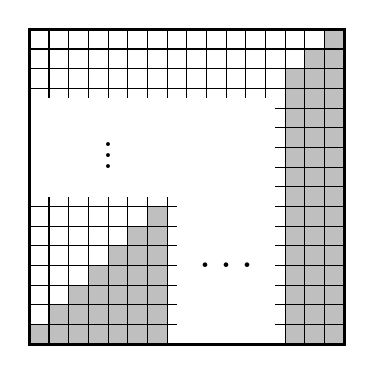
\begin{tikzpicture}[scale=0.5, x=0.5cm, y=0.5cm, font=\LARGE]
        \foreach \x in {0,...,15} 
            \foreach \y in {0,...,15}
                {
                    \pgfmathparse{(\x >= \y && (\x<7 || \x>12)) ? "lightgray" : "white"}
                    \edef\colour{\pgfmathresult}
                    \path[fill=\colour] (\x,\y) rectangle ++ (1,1);
                    \draw[black] (\x,\y) rectangle ++ (1,1);
                }
        \fill[white] (0, 7.5) rectangle ++ (8,5) node[color=black, pos=.5, align=center]{$\vdots$};
        \fill[white] (7.5, 0) rectangle ++ (5,8) node[color=black, pos=.5, align=center]{$\dots$};
        \fill[white] (7.5, 7.5) rectangle ++ (5,5) node[color=black, pos=.5, align=center]{$\iddots$};
        \draw[very thick, black] (0, 0) rectangle ++ (16,16);
    \end{tikzpicture}
\end{center}

现在,要求 $S(n)$ 的公式等价于计算正方形内所有矩形覆盖的\emph{面积}。直接相加各矩形面积只是重复原问题,因此我们需要将该面积与正方形的总面积关联。为此,考虑剩余区域,如何描述未被矩形覆盖的部分?观察第一个 $1 \times 1$ 矩形正上方的区域:它是一个尺寸为 $(n - 1) \times 1$ 的矩形。

类似地,$2 \times 1$ 矩形上方的区域是一个 $(n-2) \times 1$ 矩形。此模式持续下去!最终,在 $(n - 1) \times 1$ 矩形上方为一个 $1 \times 1$ 矩形,而最后一个 $n \times 1$ 矩形上方无区域。这些矩形的总面积类似于 $S(n)$,但缺少最后一项 $n$。现在,将所有矩形的面积与 $S(n)$ 和正方形面积关联:
\[n^2 = S(n) + (S(n) - n) = 2S(n) - n\]
解得
\[S(n) = \frac{n^2+n}{2}\]
与我们之前得到的公式一致!

\subsubsection*{解题心得}

有时,问题有多种解法。有些方法易于构思但难于求解;有些难以想到但求解简洁;还有些可能根本无效!通常无法预判哪种方法有效,因此建议动手尝试并观察结果。记录尝试的过程和结果,以便后续重新评估。这是数学学习中需牢记的原则:我们并非总能立即知晓正确路径,偶尔会陷入困境或走入死胡同。这不应令人沮丧;它是学习的一部分。

作为练习,尝试为 $n$ 为奇数的情况重新``配对'',不忽略求和的最后一项,而是分离中间项并将数字从外向内配对。这会得到相同结果吗?该方法是否比原解法更简便、更快速或有所不同呢?或者,对于 $n$ 为偶数的情况,令 $n=2k$ 会怎样?对于 $n$ 为奇数又该如何操作?这种表示会改变处理过程吗?会使问题更容易处理吗?现在,你能构思一种全新的解法吗?


% !TeX root = ../../../book.tex
\subsection{求和杂谈}\label{sec:section1.4.3}

\subsubsection*{奇数求和:观察模式}

既然谈到了整数求和,那就让我们来看一些相关的问题。首先,我们将介绍一种解释奇数之和的有趣得几何方法:让我们将 $1$ 表示为 $1 \times 1$ 块,然后将每个连续增大的奇数表示为角为 $1 \times 1$ 块的直角,完美贴合前一个这样的图。我们为什么要这样做?因为都是奇数,连续项的大小相差为 $2$,每次将角块的边延长 $1$,可以让直角与原图形紧密地相互贴合并逐渐构建起更大的正方形!

\begin{center}
    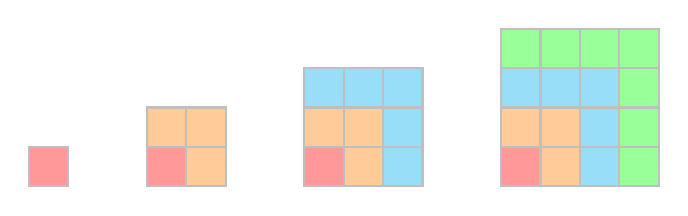
\begin{tikzpicture}[thick,scale=0.5, x=1cm, y=1cm]
        \foreach \x in {0,3,7,12}
        {
            \fill[red!40!white] (\x, 0) rectangle ++ (1,1);
            \draw[lightgray] (\x, 0) rectangle ++ (1,1);
        }

        \foreach \x in {3,7,12}
        {
            \foreach \i in {0,1}
            {
                \fill[orange!40!white] (\x+\i, 1) rectangle ++ (1,1);
                \draw[lightgray] (\x+\i, 1) rectangle ++ (1,1);
                \fill[orange!40!white] (\x+1, \i) rectangle ++ (1,1);
                \draw[lightgray] (\x+1, \i) rectangle ++ (1,1);
            }
        }

        \foreach \x in {7,12}
        {
            \foreach \i in {0,...,2}
            {
                \fill[cyan!40!white] (\x+\i, 2) rectangle ++ (1,1);
                \draw[lightgray] (\x+\i, 2) rectangle ++ (1,1);
                \fill[cyan!40!white] (\x+2, \i) rectangle ++ (1,1);
                \draw[lightgray] (\x+2, \i) rectangle ++ (1,1);
            }
        }

        \foreach \i in {0,...,3}
        {
            \fill[green!40!white] (12+\i, 3) rectangle ++ (1,1);
            \draw[lightgray] (12+\i, 3) rectangle ++ (1,1);
            \fill[green!40!white] (12+3, \i) rectangle ++ (1,1);
            \draw[lightgray] (12+3, \i) rectangle ++ (1,1);
        }
    \end{tikzpicture}
\end{center}

这种模式会持续下去吗?如果我们相信确实如此,我们如何证明这一点呢?这种几何图案的数值之和意味着什么?这是一个首先要回答的好问题,因为尽管几何图案很漂亮,但却很难使用和操作,最终也难以给出明确地\emph{证明}。本质上,对着模式的前几项说:``看,它有效!'' 并不构成官方的数学证明,因此我们必须找到更好的方法来表述这个问题。这并不是要淡化我们注意到的图案的意义和美丽;有趣的是,它的工作方式确实为我们提供了一些有价值的见解,让我们从数学上了解可能发生的事情,但归根结底,这就是它能为我们做的一切。

\subsubsection*{奇数求和:证明我们的发现}

让我们尝试用数字形式写出上图所表示的求和。 角块由 $1 \times 1$ 块组成,每个角比前一个多两块,因此我们看到的每个正方形都可以由一个和表示,例如
\[1 \:\text{ 或 }\: 1+3 \:\text{ 或 }\: 1+3+5 \:\text{ 或 }\: 1+3+5+7 \]
以此类推。我们从这些项中注意到,它们其实是平方数
\[1=1^2 \quad 1+3=4=2^2 \quad 1+3+5=9=3^2 \quad 1+3+5+7=16=4^2 \]
\emph{这}才是我们想要证明的模式;它相当于我们之前注意到的几何图案,但现在它是用我们可以操作的术语编写的。现在让我们思考一下如何才能做到这一点。这种模式与我们之前见过的模式相似吗?我们已经证明了关于整数和的结果了吗?当然!回顾之前的题目;(事实上,在某些方面)我们证明了
\[1 + 2 + 3 + \dots + (n_1) + n =\frac{n^2 + n}{2}\]
这对于该题有何用处?我们证明的求和公式涉及从 $1$ 到 $n$ 的\emph{所有}连续整数,但对于当前要求的公式,我们只想考虑连续\emph{奇数}。

之前我们用函数 $S(n)$ 表示前 $n$ 个自然数之和,所以我们定义函数 $T(n)$ 表示前 $n$ 个奇数之和。现在,我们首先需要确定该和的项,然后以某种方式将它们与 $S(n)$ 联系起来。下面,我们写出了 $n = 1,2,3 ,4$ 时的和。你能找到一种方法来识别求和中的最大项并用 $n$ 表示它吗?
\begin{align*}
    n=1: &\quad 1\\
    n=2: &\quad 1+3\\
    n=3: &\quad 1+3+5\\
    n=4: &\quad 1+3+5+7\\
\end{align*}
请注意,求和项的最后一项始终为 $2n-1$。这与一个普遍事实有关,即对于某个特定整数 $k$,任何偶数整数都可以表示为 $2k$,对于某个特定整数 $n$,任何奇数整数都可以表示为 $2n - 1$。(对于某个整数,我们也可以将奇数表示为 $2n + 1$,不过,这里使用 $2n - 1$ 更方便。)因此,我们要求的前 $n$ 个奇数之和的公式为
\[T(n) = 1 + 3 + 5 + 7 + \dots + (2n - 3) + (2n - 1)\]
我们可以将这个求和公式与 $S(n)$ 或类似的公式联系起来吗?请注意求和公式
\[S(2n) = 1 + 2 + 3 + \dots + (2n - 3) + (2n - 2) + (2n - 1) + 2n\]
包含从 $1$ 到 $2n$ 的\emph{所有}自然数,而 $T(n)$ 仅包含该范围内的奇数。也许两个和相减并尝试找到剩余项之和的表达式是有意义的:
\begin{align*}
    S(2n) - T(n) &= 1 + 2 + 3 + \dots + (2n - 1) + 2n \\
    &\quad -\big(1 + 3 + 5 + \dots + (2n - 3) + (2n - 1)\big) \\
    & =  2 + 4 + 6 + \dots + (2n - 2) + 2n
\end{align*}
这些项都是从 $2$ 到 $2n$ 的\emph{偶数}。我们怎样才能得到这个求和公式呢?我们是否需要做额外的工作,还是可以应用之前的证明结果?由于所有项都是\emph{偶数},我们可以将所有项除以 $2$ 并写成
\begin{align*}
    \frac{1}{2}\big(S(2n) - T(n)\big) &= \frac{1}{2}\big(2 + 4 + 6 + \dots + (2n - 2) + 2n\big)\\
    &= 1 + 2 + 3 + \dots + (n - 1) + n = S(n)
\end{align*}
我们可以保证,最右边的求和公式中的所有项都是整数。不仅如此,它们\emph{都是}从 $1$ 到 $n$ 的连续整数,并且我们知道它们的求和公式!现在,\text{一切都是用我们已知的公式}(即 $S(n)$ 和 $S(2n)$)以及我们要求的公式(即 $T(n)$)书写的。最后一步要做的是整理方程,分离 $T(n)$,然后代入我们已知的 $S$ 的公式:
\begin{align*}
    \frac{1}{2}\big(S(2n) - T(n)\big) &= S(n) \\
    S(2n) - T(n) &= 2S(n) \\
    T(n) &= S(2n) - 2S(n) \\
    T(n) &= \frac{(2n)^2 + 2n}{2} - \frac{2 \cdot (n^2 + n)}{2} \\
    T(n) &= \frac{4n^2 + 2n - 2n^2 - 2n}{2} \\
    T(n) &= \frac{2n^2}{2} \\ 
    T(n) &= n^2
\end{align*}
这看起来相当不错,不是吗?尽管必须完成一些代数步骤,我们还是得出了我们希望证明的结论:连续奇数的和是完全平方数。不仅如此,我们还成功地精确证明了该平方数与求和项数之间的关系。 具体来说,我们刚刚证明的结论的一种简洁概括描述是``前 $n$ 个奇数之和等于 $n^2$''。

\subsubsection*{另一种解法:归纳证明}

我们可以用不同的方式证明这一点吗?如果我们还没有证明上一节的结论,或者我们没有想到以这种方式证明它怎么办?我们能否以某种方式利用我们最初注意到的和的几何结构?

让我们回过头来用稍微不同的方式思考这个问题。具体来说,让我们看看为什么在求和中再添加一项会产生另一个平方数。假设我们已知其中一个求和产生一个平方数;我们知道这对于第一个求和 ($1 = 1^2$) 是正确的,但我们假设对于任意数量的项 $n$ 都会发生这种情况。也就是说,对于某个值 $n$, 我们\emph{假设}
\[1 + 3 + 5 + \dots + (2n - 3) + (2n - 1) = n^2\]
基于这一事实,我们接下来可以推断出下一个和是什么吗?当我们向求和中再添加一项时,我们会加上下一个奇数 $2n + 1$,所以让我们看看这会如何影响求和结果:
\[1 + 3 + 5 + \dots + (2n - 3) + (2n - 1) + (2n + 1) = n^2 + 2n + 1 = (n + 1)^2\]
这似乎证实了我们的想法,不是吗?知道求和的表现方式与我们预期的一致(``如果前 $n$ 个奇数整数之和为 $n^2$……'')我们就可以推断下一个和也必须以相同的方式表出现(……那么前 $n+1$ 个奇数整数的和是 $(n+1)^2$'')。这也证明了结论吗?你觉得怎么样?本质上假设我们的结论成立来进一步证明它,这感觉很奇怪吗?我们真的是这么做的吗?

这种证明策略 --- 使用结果的一种形式来证明结果的``后续''形式 --- 称为\textbf{数学归纳法}。(一般来说,``后续''一词的含义取决于上下文;在这里,它的意思是再加上一项后和。)我们将在下一章更详细地研究这一策略。目前,我们先指出这是一个完美的策略,但它高度依赖于第一个求和的正确表示:$1 = 1^2$。这样,我们所做的工作使我们能够推断出第二个求和是 $(1+3=2^2)$,接着就可以推断出第三个求和是 $(1+3+5=3^2)$,以此类推……如果我们只能证明第二部分,但第一部分的结果没有按照我们想要的方式计算怎么办?我们还能证明结论吗?一般来说,这对归纳策略有何启示?稍后我们将更普遍地解决其中一些问题。

\subsubsection*{泛化:算术级数}

我们要谈的最终求和问题与我们迄今为止看到的两个问题密切相关,事实上,如果我们能证明下一个结论,就不必证明前两个结论了!从这个意义上说,下一个结论比前两个结论更强:这个结论的真实性意味着前两个结论的真实性。(这是数学术语中的常见概念,将结论标记为比其他结论更强或更弱。)

对于这个结论,我们想要发展一个通用\textbf{算术级数}。这句话的意思是我们要添加一个算术级数,其中连续项之间的差是一个固定值。另一种思考方式是,每一项都是通过前一项加上一个固定常数而来。请注意,我们在后两个题目中求和的就是算术级数:第一个求和中,每项相差 $1$(或者,每项上加 $1$ 得到下一项),第二个求和中每个项相差 $2$(或者,每项上加 $2$ 得到下一项)。

我们如何表示一个通用的算术级数?因为连续项必须相差一个固定常数,让我们为该值分配一个变量,例如 $c$,作为常数。求和中也必须有第一项,所以让我们将该值分配给一个变量,例如 $a$,因为它是第一个字母。我们还需另一个变量来告诉我们求和中有多少项,因此我们将使用 $k$ 表示项数,因为我们之前已经使用过该变量表示相同的含义。现在,我们可以用这三个变量来表示整个求和:
\[A(a, c, k) = a + (a + c) + (a + 2c) + (a + 3c) + \dots + (a + (k - 2)c) + (a + (k - 1)c)\]
我们可以利用每对连续项相差 $c$ 这一事实,使用第一项 $a$ 来表示第二项,并且我们可以通过不断增加 $c$ 来表示第三项,依此类推。我们总共需要 $k$ 项,因此,将第一项视为 $a+ 0 \cdot k$,最后一项是我们将 $c$ 添加到第一项 $k - 1$ 次后得到的结果(从 $0$ 到 $k - 1$(含) 有 $k$ 个数字)。另请注意,我们引入了符号 $A(a, c, k)$ 来表示``第一项 $a$、常数差 $c$ 和 $k$ 项的算术级数之和''。现在,我们怎样才能算出这个和呢?

让我们采用以前有效的策略:在第一个求和题目中,我们正序和倒序写下求和项并将它们加在一起。这会创建许多具有相同求和结果的项对,从而将求和简化为乘法。如果我们在这里这样做时会发生什么?我们看到

\begin{center}
    \begin{tabular}{ccccccccc}
                 a & + &      (a+c) & + & \dots & + & (a+(k-1)c) & = & A(a,c,k)\\\noalign{\smallskip\smallskip}
        (a+(k-1)c) & + & (a+(k-2)c) & + & \dots & + &          a & = & A(a,c,k)\\\noalign{\smallskip\smallskip}
        \hline
        (2a+(k-1)c)& + & (2a+(k-1)c)& + & \dots & + &(2a+(k-1)c) & = &2A(a,c,k)\\\noalign{\smallskip\smallskip}
    \end{tabular}
\end{center}
我们再次发现配对项都有相同的和,在这种情况下,和是 $2a+ (k-1)c$。这样的配对项有多少对?正好是 $k$ 个项!(这就是我们选择使用该变量的原因。)将求和表示为乘法,我们现在可以推出
\[2A(a, c, k) = k \cdot (2a + (k - 1)c)\]
因此
\[A(a, c, k) = \frac{k}{2} \cdot k \cdot (2a + (k - 1)c)\]
这看起来符合你的期望结果吗?你的预期是什么?有时,尝试``猜测''可能会发生什么,然后看看结果是否与你的直觉相符,以及如何相符,会有所帮助。

\subsubsection*{具体应用}

上面提到过,我们之前题目中的求和都是算术级数,那么这个公式是否可以得出这些求和的正确结果呢?在第一题中,变量值为 $a = 1,c = 1, k = n$;代入这些值会得到
\[A(1, 1, n) = \frac{1}{2} \cdot k \cdot (2 + (n - 1)) = \frac{n}{2} \cdot(n+1) = \frac{n^2+n}{2}\]
这确实是我们之前得到的结论。那第二题呢?变量的值是多少?公式正确吗?这些问题请你来验证结果。

\subsubsection*{另一种表示}

这个问题的最后,我们想讨论另一种表示刚刚推导出的公式的方法。查看括号中的项,并以稍微不同的方式书写:$a+ (a+ (k-1)c)$。这些项看起来特别有趣吗?是的,它们分别是求和的第一项和最后一项。这为我们提供了一种不同的方式来表达我们推导出的求和公式:$A(a, c, k) = \frac{k}{2}(a + b)$,其中 $a$ 是求和的第一项,$b$ 是最后一项。这个版本的公式可以更方便,更快捷地进行一些求和。

例如,假如我们让你求一个算术级数之和,其中第一项为 $12$,最后一项为 $110$,总共有 $14$ 项,你就不必费心费力去计算常数差 $c$;相反,你可以简单地完成求和:$\frac{14}{2} \cdot (12 + 110) = 854$。是不是快得多?该算术级数的 $c$ 值是多少?给定 $a,b,k$,有没有一种简单的方法可以快速求出 $c$?

\subsubsection*{解题心得}

了解以前的结论会很有帮助,因为它们可以使证明更简短、更容易。有时,很难知道某个特定结果何时有用,或者即使意识到它的用途,也可能很难弄清楚如何应用它。在这种情况下,我们意识到到我们之前已经证明了一个求和公式,因此至少尝试弄清楚它在证明不同的求和公式时如何发挥作用是有意义的。然而,有一种完全不同的方法可以证明奇数之和的公式,不依赖于我们之前的结论。这暗示了一个更通用的结论,好奇的数学家会尝试更通用地探索这个问题,我们通过研究任意算术级数做到了这一点。但最终,我们对前两个求和公式使用了多种策略,并且仅将其中一种策略应用于一般级数问题。我们可以在其他设定下使用这些策略吗?我们是否也可以通过归纳法来证明第一个求和公式?我们可以使用正序/逆序技术来证明第二个求和公式吗?尝试使用这些策略,看看会发生什么。这对你来说可能会很奇怪或没有必要,因为我们已经有了结论,但是了解不同技术在不同环境中如何发挥作用是一个宝贵的经验。在数学中,弄清楚在证明中使用哪种策略通常与找出证明结果一样困难(甚至更难)。考虑到这一点,练习特定的策略来培养一种直觉,知道它们何时有效以及何时需要尝试其他方法,是很有帮助的。


% !TeX root = ../../../book.tex
\subsection{好友倾向}\label{sec:section1.4.4}

\subsubsection*{问题描述}

这个问题基于以下一则关于匈牙利社会学家的轶事以及他对儿童朋友圈的观察。

\begin{quote}
    ``20 世纪 50 年代,匈牙利社会学家 S. Szalai 研究了儿童之间的友谊关系。他观察到,在任何大约 $20$ 个孩子的群体中,都能找到四个孩子是共同的朋友,或者四个孩子中没有两个孩子是朋友。在得出社会学结论之前, S. Szalai 咨询了当时三位著名的匈牙利数学家: Erdos, Turan 和 Sos 。简短的讨论后表明,这其实是一种数学现象,而非社会学现象。对于至少 $18$ 个元素上的任意对称关系 $R$,存在 $4$ 个元素的子集 $S$,使得 $R$ 包含 $S$ 中的所有对或不包含其中任何对。这一事实是 1930 年证明的拉姆齐定理(Ramsey's theorem)的一个特例,拉姆齐理论的基础,后来发展成为组合数学的一个丰富领域。 --- (引自麻省理工学院 Jacob Fox 教授的\href{https://www.a.com}{讲义}。)''
\end{quote}

现在我们遵循相同的思路提出类似的问题,但数字较小。具体来说,我们想要找出\emph{满足}其中三人相互都是朋友或敌人的最小群体规模。

\begin{quote}
    假设在一群人中,其中任意两人要么是朋友,要么是敌人,并且这是唯一可能的关系(即没有熟人或亦敌亦友或类似的关系)。以四人为一组,试着为每对指定朋友/敌人关系,使得不会有三人一组都是朋友或敌人。五个人可以实现吗?六个呢?七个?十个?二十个呢?尝试确定最小群体规模,使得你就可以\emph{保证}找到一个由三个人组成的小组,他们要么都是朋友,要么都是敌人。
\end{quote} 

请仔细思考一下,然后再翻页阅读解答。

\clearpage

\subsubsection*{有效地表述问题}

你做出来了吗?这是一个非常棘手的问题,所以如果你没有解出来,请不要感到难过。事实上,我们认为调查这个问题与实际找到答案一样重要,因为有多种方法可以解决这个问题,而且看不同的人如何解释这个问题总是很有趣。

首先,让我们讨论一下如何写下/画出/谈论这种情况。对于该题提出的任何问题,我们都应该考虑一组具有一定规模的人,并思考这群人中任意两人之间的关系。为了解决这个问题,我们需要一种高效且易于解释的方法表示所有这些关系,以便我们可以验证大小为 $3$ 的子群所需的属性。具体来说,我们想要轻松识别是否存在大小为 $3$ 的\emph{同质}子群,即三个人\emph{互为}朋友或\emph{互为}敌人。从现在起,我们将其称为``\textbf{同质性}''。

我们怎么才能做到这一点呢?我们如何才能表示人及其关系呢?我们可以对小组中的人员进行编号,然后写出所有数字对的列表,并用 $F$(朋友)或 $E$(敌人)标记每对数字的关系。让我们尝试为四人小组执行此操作:

\[12F \quad 13E \quad 14F \quad 23F \quad 24E \quad 34F\]

这群朋友/敌人满足同质性吗?验证起来并不那么容易,不是吗?首先,编号使得很难找到大小为 $3$ 的子群,为了验证属性,我们需要检查所有此类子群以确保它们不是 $E E E$ 或 $F F F$。也许在尝试解决问题之前,我们应该找到一种更好的方式来表示信息。对于群体中的所有可能配对,你能想出一种视觉上令人更加愉悦的方式来表示两个人是朋友还是敌人吗?具体来说,我们希望得到一种相对有效的方法来寻找大小为 $3$ 的子群并识别它们是否全是朋友还是全是敌人。

让我们尝试将组中的每个人表示为一个点,并根据这两个人是朋友还是敌人用一种线连接两个人。例如,我们用蓝线表示朋友,用红线表示敌人(记住,任何两个人要么是朋友,要么是敌人,没有别的可能,所以每对点必然有彩色线连接它们)。例如,下图描述了我们在上面分配的关系和符号:

\begin{center}
    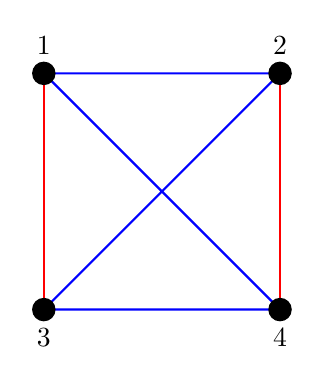
\begin{tikzpicture}[thick,scale=0.5]
        \coordinate (A) at (0,6);
        \coordinate (B) at (6,6);
        \coordinate (C) at (0,0);
        \coordinate (D) at (6,0);
        \draw[blue] (A) node[black, above, yshift=3pt]{$1$}
        -- (B) node[black, above, yshift=3pt]{$2$}
        -- (C) node[black, below, yshift=-3pt]{$3$}
        -- (D) node[black, below, yshift=-3pt]{$4$}
        -- (A);
        \draw[red] (A)--(C);
        \draw[red] (B)--(D);
        \foreach \n in {A,B,C,D}
            \node at (\n)[circle,fill,inner sep=3pt]{};
    \end{tikzpicture}
\end{center}

现在,我们要用什么方法来验证同质性?我们需要三个点(三个人),使得它们之间的所有线都是蓝色(都是朋友)或红色(都是敌人)。没错 --- 我们寻找的正是\textbf{单色三角形}!(注意:我们希望三角形的顶点是我们绘制的原始点;也就是说,我们不希望顶点是两条线的交点。此外,\emph{单色}来自希腊语 \emph{monos} 和 \emph{khroma},分别表示``一个''和``颜色''。)这种表示方式更容易直观地解释,并且可以更快地检验。

根据上图,我们解决了四人组问题:我们找到了朋友和敌人的特定排列,因此不存在全为朋友或全为敌人的三人组。也就是说,不存在具有同质性的大小为 $3$ 的子组。这表明这样的情况可以用四个人来实现,因此我们不能\emph{保证}四个人之间一定存在具有同质性的组。

你还能找到另一个这样的排列吗?你如何确定这与我们已经看到的排列\emph{不同}?有多少种不同的排列满足同质性?现在,尝试绘制一个排列,该排列\emph{一定}具有大小为 $3$ 且具有同质性的子组。那看起来会是什么样?这样的排列有多少种?

\subsubsection*{重述 $n = 5$ 的问题}

让我们继续思考由五个人组成的小组。我们的图需要发生改变,因为我们现在有五个点,这意味着需要绘制更多的线。尽管如此,我们还是会用蓝色或红色线填充所有连接,并确保没有单色三角形。这可能吗?(提示:尝试将点排列成规则的五边形形状,然后填充线。)尝试画几次,看看你的排列是否有效。随机画几条线,然后通过确保添加的新线不会创建单色三角形来指导你的选择,这也可能有帮助。

你做出来了吗?翻页看看我们是如何做的...

\clearpage

\subsubsection*{解答:$n=5$}

这是我们在五个点之间排列的红/蓝线,完全避免了同质性:

\begin{center}
    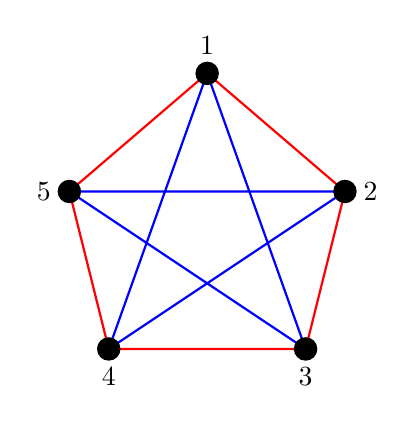
\begin{tikzpicture}[thick,scale=0.5]
        \coordinate (A) at (0,0);
        \coordinate (B) at (5,0);
        \coordinate (C) at (6,4);
        \coordinate (D) at (2.5,7);
        \coordinate (E) at (-1,4);
        \draw[red] (A) node[black, below, yshift=-3pt]{$4$}
        -- (B) node[black, below, yshift=-3pt]{$3$}
        -- (C) node[black, right, xshift=3pt]{$2$}
        -- (D) node[black, above, yshift=3pt]{$1$}
        -- (E) node[black, left, xshift=-3pt]{$5$}
        -- (A);
        \draw[blue] (A)--(D)--(B)--(E)--(C)--(A);
        \foreach \n in {A,B,C,D,E}
            \node at (\n)[circle,fill,inner sep=3pt]{};
    \end{tikzpicture}
\end{center}

请注意该图形优雅的对称性:所有红线均位于五边形的外侧,所有蓝线均位于该形状的内部。这样做的原因是,任意三个相邻点作为顶点的三角形必须使用两条外线和一条内线,任意三个不相邻点作为顶点的三角形必须使用两条内线和一条外线。(想一想:为什么我们不能用三条内线或三条外线来组成一个三角形?)这\emph{保证}了我们绘制的任何三角形都会使用两条不同颜色的线,所以这个图形不具有同质性!当然,我们可以查看图中所有可能的三角形,并确保它们都不使用一种颜色。这样的三角形有多少个?你能多快手工找到所有这些三角形?这样做是否更容易,或者注意我们上面提到的内部/外部属性?

也许你找到的解决方案与我们的图不同。你怎么知道它实际上是否是不同的图形?你的图中有多少条蓝线、多少条红线?我们的图呢?尝试通过移动点来重新绘制图形,但保持点之间的关系(即任意两个点之间绘制的线条的颜色)。你能把你的图形弄得跟我们的一样吗?你认为这对本题解的数量意味着什么?

\subsubsection*{$n=6$ 的情况}

好的,现在我们可以思考六个人的情况了。就点和线而言,我们希望用蓝色或红色线绘制六个点之间所有可能的连接,并确保不存在边都为相同颜色的三角形。在绘制前,请思考四个点和五个点时我们的解决方案。这些解是什么样的?这次我们要画多少线?我们可以试着让这个数字看起来像五个点的解决方案吗?有时,思考当前问题的解决方案与以前工作有何相似之处会大有帮助。现在,尝试画出这个图形,看看会发生什么。

有效吗?为什么无效?你在哪里遇到了麻烦?在不得不绘制单色三角形之前,你可以画多少条线?也就是说,在你绘制下一条线形成单色三角形之前,无论它是蓝色还是红色,你可以向图形中插入多少条线?某种程度上,这些问题对于解决这个特定难题来说是无关紧要的问题,但它们值得思考,因为它们本身很有趣,并且它们可能会引导我们找到这个难题的解决方案或其概括。为了便于说明,这是我们在图形中分配红线和蓝线的一种方案。我们为什么停在这里?还需要添加多少条线?我们能加进去吗?

\begin{center}
    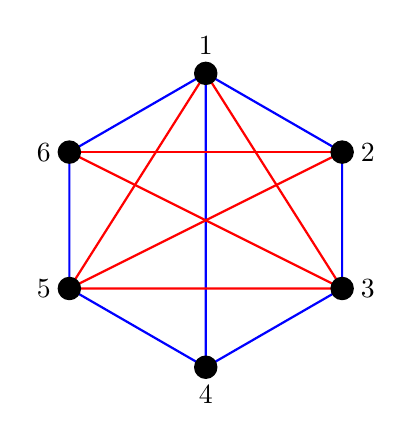
\begin{tikzpicture}[thick,scale=0.5]
        \coordinate (A) at (0,0);
        \coordinate (B) at (-3.4642,2);
        \coordinate (C) at (-3.4642,5.4642);
        \coordinate (D) at (0,7.4642);
        \coordinate (E) at (3.4642,5.4642);
        \coordinate (F) at (3.4642,2);
        \draw[blue] (A) node[black, below, yshift=-3pt]{$4$}
        -- (B) node[black, left, xshift=-3pt]{$5$}
        -- (C) node[black, left, xshift=-3pt]{$6$}
        -- (D) node[black, above, yshift=3pt]{$1$}
        -- (E) node[black, right, xshift=3pt]{$2$}
        -- (F) node[black, right, xshift=3pt]{$3$}
        -- (A)
        -- (D);
        \draw[red] (B)--(E);
        \draw[red] (C)--(F);
        \draw[red] (B)--(D)--(F)--(B);
        \draw[red] (C)--(E);
        \foreach \n in {A,B,C,D,E,F}
            \node at (\n)[circle,fill,inner sep=3pt]{};
    \end{tikzpicture}
\end{center}

我们现在面临的情况很有趣,因为它与我们之前面临的情况性质相反。在四个点和五个点的情况中,我们想表明\emph{可以}通过排列所有线来消除单色三角形。为了证明这一点,只需画出来就好!画出具有所需属性的\emph{特定}图形就足以证明可以实现我们想要的属性。然而,对于六个点,似乎不可能将线条排列得不存在单色三角形。我们怎样才能证明这是事实呢?我们很容易想到,只需考虑线条的所有可能排列,并论证每一中排列中至少有一个单色三角形。这可行吗?线条有多少种排列方式?我们如何在任意给定图形中轻松找到单色三角形?还记得我们对五个点的图形进行此操作吗?我们注意到,任何三角形都必须使用\emph{至少}一条来自外部的线和\emph{至少}一条来自内部的线,这保证了任何三角形都有两种类型的线。我们可以在这里做同样的事情,并明确一些\emph{保证}存在非单色三角形的性质吗?

问题是,图中六点之间线的可能排列方式太多了,我们无法手动完成所有检查!这里有 $15$ 条线需要绘制,每条线都可以是蓝色或红色,因此共有 $2^{15}$ 种可能的排列。这是一个很大的数字!(实际上,排列可能性会稍微少一些,因为其中一些排列在某种意义上是等价的;更专业地说,它们是``\emph{同构的}''。)

\subsubsection*{解答:处理\emph{任意}图形}

我们需要更巧妙地进行论证,这样我们就可以在不绘制特定图形的情况下证明\emph{任意}图形的性质。也就是说,我们需要找到一些事实,一些对所有可能的六点图都成立的性质,但我们仍然能够推断出一定存在三角形。解决这个问题的一种方法是考虑在图形的一小部分中绘制线条。具体来说,让我们取六个点中的任意一个,并考虑从该点引出的五条线。例如,我们可能会得到下面的图形:

\begin{center}
    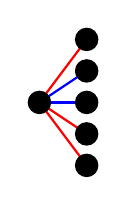
\begin{tikzpicture}[thick,scale=0.2]
        \coordinate (A) at (0,0);
        \coordinate (B) at (3,2);
        \coordinate (C) at (3,0);
        \coordinate (D) at (3,4);
        \coordinate (E) at (3,-2);
        \coordinate (F) at (3,-4);
        \draw[blue] (A)--(C);
        \draw[blue] (A)--(B);
        \draw[red] (A)--(D);
        \draw[red] (A)--(E);
        \draw[red] (A)--(F);
        \foreach \n in {A,B,C,D,E,F}
            \node at (\n)[circle,fill,inner sep=3pt]{};
    \end{tikzpicture}
\end{center}

有多少蓝线,多少红线?这在一定程度上是一个棘手的问题:我们并没有真正考虑任何\emph{特定}图形(如上面的图形),而是试图找到有关所有可能图形的事实。因此,我们不能太具体地回答这个问题。假设我们看到一个\textbf{任意}图形,我们必须提出一个无论该图形是什么都有效的论证。 

我们\emph{可以}这样说:必须至少有三条蓝线或三条红线。你明白为什么这是真的吗?使其不成立的唯一方法是从特定点出发,有两条(或更少)蓝线和两条(或更少)红线,共计四条(或更少)线。不过,我们必须画出所有可能的连接,因此应该有五条!(这个论证是``\emph{抽屉原理}''的一个例子。这个原理说的是,我们无法将两种不同颜色的五个物体放入两个不同盒子中,而不将三个同种颜色的物体放入一个盒子。对这类问题来说,抽屉原理是一个非常有用的策略,我们稍后将在 \ref{sec:section8.6} 节更详细地研究该原理。)

那么我们的立场是什么呢?我们从任意一个六个点、填满线的图形开始,到专注于一个特定的点;从这个点出来,一定有三条蓝线或三条红线。它可以是任意一种颜色,所以我们不能仅仅假设它是红色的并遵循这种假设进行论证;我们可以这样做,但之后必须回到这一点,看看如果这三条线是蓝色的,会发生什么变化。因此,让我们这样处理:让我们检查所有有三条红线从该特定点引出的图形。我们能得到什么?我们还没有对图中的其他线做出任何假设,所以让我们看看它们可能是什么。观察下图,看看到目前为止我们假设存在哪些线条颜色:

\begin{center}
    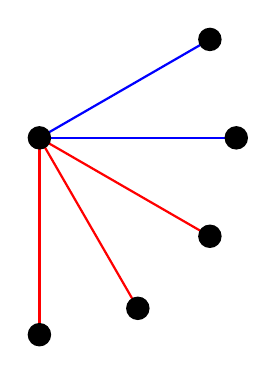
\begin{tikzpicture}[thick,scale=0.5]
        \coordinate (A) at (0,0);
        \coordinate (B) at (4.33,2.5);
        \coordinate (C) at (5,0);
        \coordinate (D) at (4.33,-2.5);
        \coordinate (E) at (2.5,-4.33);
        \coordinate (F) at (0,-5);
        \draw[blue] (A)--(C);
        \draw[blue] (A)--(B);
        \draw[red] (A)--(D);
        \draw[red] (A)--(E);
        \draw[red] (A)--(F);
        \foreach \n in {A,B,C,D,E,F}
            \node at (\n)[circle,fill,inner sep=3pt]{};
    \end{tikzpicture}
\end{center}

现在,可以在该图中添加哪些线而不会在三点之间形成同种颜色的三角形?我们不能对图中两个孤立点之间的线做任何假设,所以让我们关注底部的三个点。其中的线条可能是什么颜色?如果其中任何一条是红色的,那就会在该线的两个端点和我们关注的原始点之间形成一个单色三角形!这是有问题的。

\begin{center}
    \begin{tikzpicture}[thick,scale=0.5]
        \coordinate (A) at (0,0);
        \coordinate (B) at (4.33,2.5);
        \coordinate (C) at (5,0);
        \coordinate (D) at (4.33,-2.5);
        \coordinate (E) at (2.5,-4.33);
        \coordinate (F) at (0,-5);
        \draw[blue] (A)--(C);
        \draw[blue] (A)--(B);
        \draw[red] (A)--(D);
        \draw[red] (A)--(E);
        \draw[red] (A)--(F);
        \draw[red] (E)--(F);
        \draw [red,-stealth,very thick] (-2,-2.4) node[red, above]{$\text{红色三角形}$} -- (1,-3.5);
        \foreach \n in {A,B,C,D,E,F}
            \node at (\n)[circle,fill,inner sep=3pt]{};
    \end{tikzpicture}
\end{center}

避免这种情况的唯一方法是将所有这些线都变成蓝色。但这会在这三个点之间形成一个蓝色三角形!哇,看来无论我们做什么都无法避免生成单色三角形!

\begin{center}
    \begin{tikzpicture}[thick,scale=0.5]
        \coordinate (A) at (0,0);
        \coordinate (B) at (4.33,2.5);
        \coordinate (C) at (5,0);
        \coordinate (D) at (4.33,-2.5);
        \coordinate (E) at (2.5,-4.33);
        \coordinate (F) at (0,-5);
        \draw[blue] (A)--(C);
        \draw[blue] (A)--(B);
        \draw[red] (A)--(D);
        \draw[red] (A)--(E);
        \draw[red] (A)--(F);
        \draw[blue] (F)--(D)--(E)--(F);
        \draw [blue,-stealth,very thick] (5.5,-3.8) node[blue, right]{$\text{蓝色三角形}$} -- (2.5,-3.8);
        \foreach \n in {A,B,C,D,E,F}
            \node at (\n)[circle,fill,inner sep=3pt]{};
    \end{tikzpicture}
\end{center}

让我们回到抽屉原理并重新评估情况。如果原理保证的相同类型的三条线是蓝色而不是红色会怎样?其实,不会有什么改变。向图形底部的三个点之间添加新线,我们仍然会陷入困境:

\begin{center}
    \begin{tikzpicture}[thick,scale=0.5]
        {
            \coordinate (A) at (0,0);
            \coordinate (B) at (4.33,2.5);
            \coordinate (C) at (5,0);
            \coordinate (D) at (4.33,-2.5);
            \coordinate (E) at (2.5,-4.33);
            \coordinate (F) at (0,-5);
            \draw[red] (A)--(C);
            \draw[red] (A)--(B);
            \draw[blue] (A)--(D);
            \draw[blue] (A)--(E);
            \draw[blue] (A)--(F);
            \draw[blue] (E)--(F);
            \draw [blue,-stealth,very thick] (-2,-2.4) node[blue, above]{$\text{蓝色三角形}$} -- (1,-3.5);
            \foreach \n in {A,B,C,D,E,F}
                \node at (\n)[circle,fill,inner sep=3pt]{};
        }
        {
            \coordinate (A1) at (8,0);
            \coordinate (B1) at (12.33,2.5);
            \coordinate (C1) at (13,0);
            \coordinate (D1) at (12.33,-2.5);
            \coordinate (E1) at (10.5,-4.33);
            \coordinate (F1) at (8,-5);
            \draw[red] (A1)--(C1);
            \draw[red] (A1)--(B1);
            \draw[blue] (A1)--(D1);
            \draw[blue] (A1)--(E1);
            \draw[blue] (A1)--(F1);
            \draw[red] (F1)--(D1)--(E1)--(F1);
            \draw [red,-stealth,very thick] (13.5,-3.8) node[red, right]{$\text{红色三角形}$} -- (10.5,-3.8);
            \foreach \n in {A1,B1,C1,D1,E1,F1}
                \node at (\n)[circle,fill,inner sep=3pt]{};
        }
    \end{tikzpicture}
\end{center}

如果我们加入任何蓝色线,它就会与原始点形成一个单色三角形,如果我们将它们全部变成红色,就会在那三个点间形成一个单色三角形!从这个意义上讲,我们在抽屉原理之后遵循的两个论证是\emph{相同的}。如果我们用``红色''替换``蓝色''一词,反之亦然,我们会得到相同的论点。有时,数学家会利用这种情况来简化证明,只说``不失一般性,三条线是红色的''。这通常意味着,如果我们做出其他选择(即,如果线是蓝色的),那么进一步的论证在数学上将具有相同的结构,因此我们可以不重复书写相同的文字来节省时间和空间。事实上,这种情况非常常见,以至于有时你可能会看到``不失一般性''这个短语缩写为 \textbf{WOLOG} 或 \textbf{WLOG}。

\subsubsection*{解答:总结结果}

到目前为止我们取得了什么成果?我们绘制了\emph{特定}的图形,表明我们可以将线条排列在四个和五个点之间,而不出现单色三角形,并且我们认为\emph{任何}由六个点构成的图\emph{一定}具有单色三角形。就题目中朋友/敌人的表述而言,这意味着任何六人组必然存在一个三人组,其中的成员要么都是朋友要么都是敌人。

请注意,把这个问题改写成这个点/线的形式是多么有帮助;它让我们完全忘记了问题的社交背景(某种程度上,这可能会分散注意力),并简化了术语和符号(我们将成对的人标记为``朋友''或``敌人''变为简单地绘制两点之间一条线)。这是一个非常有用的策略:提取谜题的内在结构 --- 底层工作、元素之间的关系、它们如何相互作用等 --- 并根据这些部分重写所有内容。这可以使难题变得更容易理解和解决,并且可以指导我们设计更好的符号。如果我们继续用 $13F, 23E, \dots$ 这种符号来解决这个问题会怎样?也许最终能解决,但会困难得多!

这个题目最初的问题之一是确定一个下界,使得任何更大的人群都必然拥有该子群属性。你认为我们已经做到了吗?我们确定了一个下界了吗?六可能是这个数字吗?为什么是或为什么不是?在任意七人组中,都有一个较小的六人组,而我们上面的工作证明该小组中必然存在三个共同的朋友/敌人!当然,这适用于任何人数超过六人的群体,因此这一定是我们要寻找的精确下界。这与题目原始陈述中提到的结果类似,匈牙利社会学家在规模为四的子群中注意到了这种现象。这个问题解决起来要困难得多,所以我们这里解决了一个更小、更简单的案例。这两个结果都与称为\textbf{拉姆齐理论}的一大类问题有关。组合学和图论的这个分支致力于识别这些``下界'',随着某种结构(如一群人)的规模不断增长,最终会出现一个点,我们可以\emph{保证}找到一个具有某种属性的子群(三个共同的朋友/敌人)。起初被认为是一种社会学现象,后来被证明是严格的数学事实。牛不牛!

\subsubsection*{泛化:留给你的问题}

在继续之前,让我们提出一些有趣且相关的问题。如果我们要寻找不同规模的同质群(例如四个、五个或十二个)该怎么办?当然,总的来说,我们必须有更多的人才能保证找到这样的子群。我们可以一直这样做吗?也就是说,给定任何所需的子群大小,我们可以像上面那样确定一个下界吗?即使没有找到特定的数字,你能想出如何证明这样的下界一定存在吗?此外,如果我们允许第三种可能:朋友、敌人、陌生人,又会怎样呢?我们可以回答关于同质群的类似问题吗?这些都与拉姆齐理论相关,甚至其中一些问题相当难以回答,需要数学家多年努力才能解决。许多此类简单问题仍然是悬而未决的、未解难题!如果你在这些问题上没有任何进展,请不要灰心。我们相信,对这些问题的任何尝试和思考都是有意义且有益的。

\subsubsection*{解题心得}

这个问题带来了几个困难。首先,我们必须找到一种方法来以有意义的方式解释谜题,以便我们可以解决这个问题,这涉及到提出适当的符号来表示题目的元素。这是解决数学问题的重要组成部分,特别是这种不将符号和可视化作为问题陈述一部分的问题。

其次,为了确定 6 是群规模下界,我们必须以某种方式证明某些事情是\emph{不}可能的,但要检验的可能情况数量太大,无法单独检验每种情况。这种情况经常发生,特别是在与计算机科学和算法相关的问题中。为了解决这个问题,我们必须采用一种比大力出奇迹更巧妙的策略,而且并不总是清楚该采取什么策略。在这里,我们先是尝试填入线,就好像它会成功一样,然后意识到我们已经达到了一个无法添加的地步。证明某件事是可能的,相当于只是展示该现象的一个例子(我们对四人和五人组就是这么做的),但证明某件事是\emph{不可能}的可能要棘手得多,并且需要一些依赖上下文的独创性。

最后,我们发现,思考与当前问题密切相关的问题可能会很有趣,这些相关问题往往只需调整原问题的一个或多个条件。如果我们寻找更大的子群怎么办?如果我们允许更多类型的线怎么办?这将如何改变结果?通过改变这些条件来探索问题的边界可以带来新的数学发现和技术,并促使数学家积极探寻新的知识和分享知识的方法。

\clearpage


% !TeX root = ../../../book.tex
\subsection{三门问题}

\subsubsection*{问题描述}

这个问题仅涉及基础概率与算术,但多年来却让无数聪明人折戟沉沙。1990 年,玛丽莲·沃斯·萨万特 (Marilyn vos Savant) 在《Parade》杂志专栏发表该问题及其解法后,引发了激烈争论,许多人(包括数学家)致信赞同或反对她(正确)的答案。让我们看看你的见解!

\begin{quote}
    假设你正在参加一档游戏节目,面前有三扇门。其中一扇门后是汽车,其余两扇后是山羊。游戏开始前,汽车和山羊的位置已被随机放置在门后。游戏规则如下:你选定一扇门后,该门暂时保持关闭。主持人蒙蒂·霍尔 (Monty Hall) 知晓门后的情况,他会打开其余两扇门中有山羊的一扇。若两扇门后皆为山羊,他会随机开启一扇。蒙蒂·霍尔打开一扇有山羊的门后,会询问你:是坚持最初的选择,还是切换至另一扇关闭的门?试想:你选择了 1 号门,主持人打开了藏有山羊的 3 号门,然后问你:``是否要换到 2 号门?''改变最初的选择对你有利吗?
\end{quote}

当然,我们假设你更希望赢得汽车而非山羊,且力求最大化获胜概率。值得一提的是,该问题得名于电视节目《\emph{Let's Make a Deal}》的主持人蒙蒂·霍尔 (Monty Hall)。

那么你怎么想?试想自己站在聚光灯下,面对所有观众,当蒙蒂·霍尔问你:``要换到另一扇门吗?'' 你会作何选择?

请仔细思考一下,然后再翻页阅读解答。

\clearpage

\subsubsection*{结论:\emph{坚决}切换}

我们直接给出结论——该结论可能令人惊讶:你应当改变最初的选择!推理过程才是棘手且令人困惑的部分,而如何建立正确的解题思路正是该问题长期困扰求解者的原因。

\subsubsection*{错误论证分析}

首先展示一个常见的错误``解答'',该解答声称换门与否无关紧要。假设你与朋友讨论此题时对方提出如下解释,你会如何回应?该论证是否成立?若不同意,你会如何指出其谬误?

\begin{quote}
    当我选定一扇门后,蒙蒂·霍尔展示了另一扇有山羊的门,此时只剩两扇关闭的门。一扇后有山羊,另一扇后有汽车,因此我最初选择的门后有汽车的概率为 $50\%$,另一扇门后有汽车的概率也为 $50\%$。因此,换门不换门没有区别,还不如坚持最初的选择。
\end{quote}

上面的解释能说服你吗?让我们揭示其根本缺陷。解决此问题的关键在于计算两个概率值:坚持原选择获胜的概率,以及换门后获胜的概率。唯有准确计算并比较这两个值,才能彻底解决这个难题。

上述论证将两个概率均视为 $50\%$,但其推理存在根本缺陷。你认为坚持原选择获胜的真实概率是多少?关键在于:展示有山羊的门的行为并不会影响最初选择的门后的物体。请重点理解以下陈述:

\begin{quote}
    因为有三扇门,所以一开始选择正确的门的概率是 $\frac{1}{3}$,看到另一扇门后面有山羊\emph{并不能改变这一事实}。
\end{quote}
这正是上面错误论证的核心症结,也是``解答''本题时最常见的误区。

接下来计算换门后的胜率,并将其与 $\frac{1}{3}$ 进行比较。事实上,有多种方法可以计算此概率。一种简洁的推导是:只要初始选择的门后是山羊(概率 $\frac{2}{3}$),换门必然获胜(赢得汽车)。因为此时两扇未选门中藏着山羊与汽车,主持人必定展示有山羊的门,剩余那扇门后必定是汽车。因此换门策略的胜率为 $\frac{2}{3}$。

\subsubsection*{枚举可能性}

上述解释可能无法令你信服,我们不妨尝试实际枚举门后山羊与汽车的可能排列,并具体分析每种情况下切换选择的结果。首先请注意,门的编号并无实质影响,因为所有选择都是随机的;也就是说,无论汽车停在 1 号门、2 号门还是 3 号门后,我们最初选中汽车的概率始终是 $\frac{1}{3}$。因此可 \textbf{WOLOG}(此缩写意为``不失一般性'')假设汽车位于 1 号门后,山羊分别在 2 号门和 3 号门后。需要强调的是,这是我们自己设定的条件,参赛者并不知晓(否则必然直接选择 1 号门!)。基于此设定,我们考察初始选择的全部三种情况:

\begin{center}
    \begin{tabular}{ c|c|c } 
     1 号门 & 2 号门  & 3 号门 \\ 
     \hline 
     汽车   & 山羊    & 山羊 \\
    \end{tabular}
\end{center}

\begin{center}
    \begin{tabular}{ c|c|c|c } 
     我们的选择 & 主持人展示 & 换门结果 & 不换门结果 \\ 
     \hline 
     1 号门    & 2 号门 \:或\: 3 号门  & 山羊 & 汽车 \\
     2 号门    & 3 号门            & 汽车 & 山羊 \\
     3 号门    & 2 号门            & 汽车 & 山羊 \\
    \end{tabular}
\end{center}

关键发现在于:当我们初始选中有汽车的门时,主持人可以随机开启任意一扇有山羊的门。但无论开启哪扇门,切换选择都将失败,而坚持选择会获胜。这种情况仅占 $\frac{1}{3}$,即初始选中汽车的概率。由于表中所有情况概率均等,可以得出结论:切换策略的胜率为 $\frac{2}{3}$,而坚持策略的胜率仅为 $\frac{1}{3}$。

现在是否感觉问题更清晰了?不妨向亲友提出这个问题并观察他们的反应:有多少人答对?多少人能正确解释?多少人误答``概率相同''?又有多少人此前已经接触过此题?

\subsubsection*{泛化到多门多车情形}

让我们将这个游戏节目问题泛化,分析切换策略是否仍然有效。假设共有 $n$ 扇门和 $m$ 辆汽车,因此有 $n - m$ 只山羊。为进行有效分析,需满足 $m \le n - 2$,原因如下:

\begin{itemize}
    \item 如果 $m = n$,则无论切换与否都必然获胜,无需讨论。
    \item 如果 $m = n-1$,当初始选择有山羊的门时,主持人\emph{无法}展示另一扇有山羊的门,游戏规则无法成立,切换策略也就毫无意义。
\end{itemize}

现在,有了这些变量,游戏的新规则如下:我们随机选择一扇门。主持人从\emph{其余}门中随机打开一扇有山羊的门。此时可选择坚持最初选择或切换至\emph{任意}未打开的门。关键问题是:最优策略是什么?切换是否有利?答案是否取决于 $m$ 和 $n$?

我们将用与原题中第一种方法大致相同的方式来处理这道修改后的问题。由于 $m,n$ 为变量,我们无法枚举所有情况,只能采用逻辑推理来推断坚持和切换的胜率。首要观察与原始问题一致:\emph{坚持策略}的胜率等于初始选中汽车的概率。若初始选中有汽车的门(概率 $\frac{m}{n}$),坚持必胜;若选中有山羊的门(概率 $\frac{n-m}{n}$),坚持必败。故坚持策略的胜率为 $\frac{m}{n}$。

为了计算切换策略的胜率,需要分两种情况讨论。请注意,当 $m \geq 2$ 时,初始选中有汽车的门后切换仍可能获胜。考虑到这一点,我们需要分两种不同情况讨论:(a) 初始选中有山羊的门的情况,(b) 初始选中有汽车的门的情况。每种情况都会给主持人留下不同数量的选择,进而留下不同数量的切换策略和获胜方式,所以此处需要分开处理。

\begin{enumerate}[label=(\alph*)]
    \item \textbf{初始选中有山羊的门}。现在还剩下 $n - m - 1$ 扇有山羊的门,主持人随机选择其中一扇打开。从我们的角度来看,切换给我们留下了 $n-2$ 个选项(我们不能切换到已打开的门和最初选择的门),其中 $m$ 个是汽车。因此,在这种\emph{特定}情况下,切换后获胜的概率为 $\frac{m}{n-2}$。\\
    由于最初有 $n - m$ 只山羊,所以这种情况发生的概率为 $\frac{n-m}{n}$。因此,这种情况对切换后总获胜概率的贡献为
    \[\frac{n-m}{n} \cdot \frac{m}{n-2} = \frac{nm-m^2}{n(n-2)}\]
    (思考一下为什么我们要把这些概率相乘而不是相加?我们要如何将此概率与下一种情况的概率结合起来?)
    \item \textbf{初始选中有汽车的门}。现在还剩下 $n - m$ 扇有山羊的门,主持人随机选择其中一扇打开。从我们的角度来看,切换给我们留下了 $n-2$ 个选项,其中 $m - 1$ 个是汽车。因此,在这种\emph{特定}情况下,切换后获胜的概率为 $\frac{m-1}{n-2}$。\\
    由于最初有 $m$ 辆车,所以这种情况发生的概率为 $\frac{m}{n}$。因此,这种情况对切换后总获胜概率的贡献为
    \[\frac{m}{n} \cdot \frac{m-1}{n-2} = \frac{m^2-m}{n(n-2)}\]
\end{enumerate}

由于这两种情况是独立发生的(即它们不可能同时发生),我们需要将这两个概率相加,从而得到切换策略的总胜率:
\begin{align*}
    \frac{nm-m^2}{n(n-2)} + \frac{m^2-m}{n(n-2)} &= \frac{nm - m^2 + m^2 - m}{n(n-2)} \\
    &= \frac{nm - m}{n(n-2)} \\
    &= \frac{m(n - 1)}{n(n-2)} \\
    &= \frac{m}{n} \cdot \frac{n-1}{n-2}
\end{align*}
将此结果与坚持策略的胜率 $\frac{m}{n}$ 比较。因为 $ n - 1 > n - 2$,所以 $\frac{n-1}{n-2} > 1$,可得不等式:
\[\frac{m}{n} < \frac{m}{n} \cdot \underbrace{\frac{n-1}{n-2}}_{>1}\]
切换策略的胜率\emph{严格大于}(即总是大于)坚持策略的胜率。因此,随机切换到另一扇门总是更优策略!

\subsubsection*{具体应用}

此问题的原始版本对应 $n = 3$ 且 $m = 1$,因此可以将这些值代入来验证结果的正确性。根据推导公式,坚持策略的胜率为 $\frac{1}{3}$,而切换策略的胜率为 $\frac{1(3-1)}{3(1)} = \frac{2}{3}$,与之前的结论完全吻合!

\subsubsection*{泛化:留给你的问题}

当 $m$ 和 $n$ 取其他值时会发生什么?能否使``始终切换''策略显著优于``始终坚持''策略?两种策略的胜率差异最大能达到多少?最小又能缩小至何种程度?是否存在使两者胜率相等的情况?

该问题的另一变体是主持人开启多于一扇有山羊的门。具体设定如下:共有 $n$ 扇门,其中 $m$ 扇后有汽车;玩家首次选择后,主持人从剩余门中随机开启 $p$ 扇有山羊的门;此时玩家可选择坚持初始选择,或切换到未开启的 $n-p-1$ 扇门中的任意一扇。在此情形下最优策略是什么?需对 $m,n,p$ 施加何种约束条件以保证游戏成立?最优策略是始终切换,还是取决于 $p$ 的取值?``始终切换''与``始终坚持''策略的胜率差异范围如何?

\subsubsection*{解题心得}

直觉和快速决策有时能\emph{引导}我们找到正确答案,但务必检查这些仓促判断是否基于合理的逻辑。本题中,``$50/50$''的概率初看似乎成立,但仔细推敲后便发现其论证存在缺陷——关键在于正确解读题目并严格遵循游戏步骤的顺序。概率分析应按照游戏实际发生的流程进行,而非从结果倒推。

概率问题往往极具迷惑性,需格外审慎对待。这也揭示了一个深刻启示:看似简单的问题往往最难攻克。切勿因表述简短或易于理解而轻视问题的复杂性!

关于蒙蒂·霍尔问题及其心理学背景,请参见 \href{http://www.usd.edu/~xtwang/Papers/MontyHallPaper.pdf}{Krauss, Stefan and Wang, X. T. (2003). ``The Psychology of the Monty Hall Problem: Discovering Psychological Mechanisms for Solving a Tenacious Brain Teaser'', \emph{Journal of Experimental Psychology}: General 132(1)}。

\newpage
% !TeX root = ../../../book.tex
\section{学而时习之}\label{sec:section1.5}

我们以一些练习结束本章,这些练习既包含讨论过的概念,又能让你实践所学知识,同时可以让你保持思维敏捷。请尽可能尝试解答,并与朋友探讨解题思路。不过,归根结底,把这些练习当作一种保持大脑灵活的方式就好!\\

\begin{exercise}
    一只苍蝇停在一辆以 $60$ 公里/小时的速度行驶的火车前端。同轨道前方 $300$ 公里处,另一列火车正以 $60$ 公里/小时的速度迎面驶来。当两车相距 $300$ 公里时,苍蝇以 $90$ 公里/小时的速度起飞,在火车间的轨道上来回飞行,到达火车时瞬间转向。当两车相撞挤压苍蝇时,苍蝇共飞行了多少距离?你是如何求解的?尝试推广到一列火车时速 $a$ 公里,另一列火车时速 $b$ 公里,苍蝇时速 $c$ 公里。
\end{exercise}

\begin{exercise}
    政府铸币厂受委托铸造一批金币。铸币厂有 $20$ 台机器,每台机器生产重 $5$ 克的金币。某日工头发现部分金币偏轻,经检查发现有一台机器铸造出的金币为 $4$ 克,其余 $19$ 台机器正常。他决定化不利为有利,借此选拔最聪明的员工进行提拔。工头告知工人:仅有一台机器生产的金币为 $4$ 克,且仅允许用秤称量一次。作为员工,你可选取任意选定机器生产的任意数量的金币,但需合并称重并读取总克数。如何准确找出故障机器?
\end{exercise}

\begin{exercise}
    在国际象棋中,皇后可以沿垂直、水平或对角线方向移动任意格数。在标准 $8 \times 8$ 棋盘上放置 $8$ 个皇后,要求任意皇后均无法攻击其他皇后(即\emph{不存在}皇后可在一步内吃掉另一皇后)。请给出一种解法或证明其不可能性。若存在解法,试讨论共有多少种不同放置方式;若不可能,请确定棋盘上最多可放置多少个满足条件的皇后。
\end{exercise}

\begin{exercise}
    在标准 $8 \times 8$ 棋盘上去除对角位置的两个方格(例如左上角和右下角)。能否用 $2 \times 1$ 多米诺骨牌不重叠地覆盖所有剩余方格(即实现棋盘\emph{密铺})?请说明理由。推广至 $n \times n$ 棋盘,该结论是否依赖 $n$ 的取值?请解释原因。
\end{exercise}

\begin{exercise}
    考虑标准 $8 \times 8$ 棋盘,移除两个相邻的对角方格(如图所示)。能否用 T 形四联骨牌密铺该棋盘?若可行,请描述方法;若不行,请解释原因。

    \begin{center}
        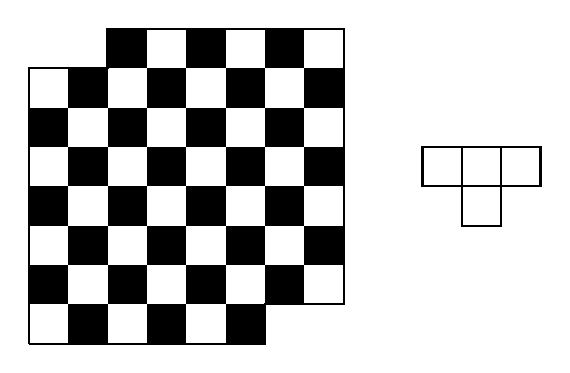
\begin{tikzpicture}[thick, scale=0.5, x=1cm]
            \foreach \x in {0,...,5}
                {
                    \pgfmathparse{mod(\x,2) ? "black" : "white"}
                    \edef\colour{\pgfmathresult}
                    \path[fill=\colour] (\x, 0) rectangle ++ (1,1);
                }
            \foreach \x in {0,...,7} 
                \foreach \y in {1,...,6}
                    {
                        \pgfmathparse{mod(\x+\y,2) ? "black" : "white"}
                        \edef\colour{\pgfmathresult}
                        \path[fill=\colour] (\x,\y) rectangle ++ (1,1);
                    }
            \foreach \x in {2,...,7}
                {
                    \pgfmathparse{mod(\x+1,2) ? "black" : "white"}
                    \edef\colour{\pgfmathresult}
                    \path[fill=\colour] (\x, 7) rectangle ++ (1,1);
                }
            \draw (0,0)--(6,0)--(6,1)--(8,1)--(8,8)--(2,8)--(2,7)--(0,7)--(0,0);
            \draw (10,4) rectangle ++ (1,1);
            \draw (11,4) rectangle ++ (1,1);
            \draw (12,4) rectangle ++ (1,1);
            \draw (11,3) rectangle ++ (1,1);
        \end{tikzpicture}
    \end{center}
    推广至 $n \times n$ 棋盘,该结论是否依赖 $n$ 的取值?请说明理由。
\end{exercise}

\begin{exercise}
    给定实数 $x$,定义 $\lfloor x \rfloor$ 为小于或等于 $x$ 的最大整数,$\lceil x \rceil$ 为大于或等于 $x$ 的最小整数。例如,$\lfloor 6.02 \rfloor = 6, \lfloor 6.99999 \rfloor = 6, \lfloor 6 \rfloor = 6, \lfloor -6.5 \rfloor = -7$。尽可能为以下表达式的值找到更具体和简洁的表示形式。(你可能需要根据 $x$ 的值给出不同表达式。)

    \begin{enumerate}
        \item $\lfloor x \rfloor + \lfloor 1-x \rfloor$ 
        \item $\lceil x \rceil + \lceil 1-x \rceil$
        \item $\lfloor x \rfloor + \lceil x \rceil$
        \item $\frac{\lfloor x \rfloor}{x}$
        \item $\lfloor x^2 \rfloor - \lfloor x \rfloor ^2$
        \item $\lceil x^2 \rceil - \lceil x \rceil^2$
    \end{enumerate}
\end{exercise}

\begin{exercise}
    求三个自然数 $a,b,c$,使得没有子集之和能被 $3$ 整除。即求 $a,b,c$ 满足以下和均不被 $3$ 整除:$a,b,c,a + b,a + c,b + c,a + b + c$。这可能吗?为什么?\\
    \\
    尝试用 $4$ 个数做同样的事:求自然数 $a,b,c,d$,使得没有子集之和能被 $4$ 整除。这可能吗?为什么?\\
    \\
    尝试推广:你能说明如何找到 $n$ 个自然数,使得所有子集之和都不能被 $n$ 整除吗?
\end{exercise}

\begin{exercise}
    回顾通过点和彩色连线解决朋友倾向问题的方法。这里我们考虑类似情形:给定若干点,需绘制所有可能线段,使得任意两点恰由一条线段连接,但忽略颜色(所有线段可视为黑色)。你能用 $3$ 个点画出该图形且所有线段不交叉吗?$4$ 个点呢?$5$ 个点呢?$6$ 个点呢?为什么可以或为什么不可以?尝试解释为什么某些图形不可能实现。若无法达成 $0$ 次交叉,可能达到的最小交叉次数是多少?
\end{exercise}

\begin{exercise}
    画一个圆,沿圆周放置 $3$ 个点。现需对点之间的圆弧着色(每段一种颜色),要求相邻圆弧的颜色不同。至少需要多少种颜色?若放置 $4$ 个点呢?$5$ 个点呢?尝试推广到 $n$ 个点的情况。你能说明所需颜色的最小数量吗?
\end{exercise}

\begin{exercise}
    假设你有一个装满袜子的抽屉,其中有 $2$ 双蓝色袜子、$3$ 双红色袜子和 $4$ 双绿色袜子(左右袜不可区分)。某天清晨你匆忙随机抓取袜子,每次一只,直至手中凑成一双为止。为\emph{保证}获得一双袜子,至少需要从抽屉中取出多少只?\\
    \\
    若每种颜色的袜子数量加倍,答案如何变化?若共有红、绿、蓝、黄、棕五种颜色,每种颜色 $3$ 双呢?推广到 $m$ 种颜色,每种颜色 $n$ 双的情况呢?
\end{exercise}

\begin{exercise}
    深夜,四人行至一座老旧摇晃的桥前。此桥最多同时承载两人,且需手电筒照明。四人过桥所需时间分别为 $5$ 分钟、$10$ 分钟、$15$ 分钟和 $20$ 分钟。两人同行时,按较慢者速度通过。四人全部过桥的最短时间是多少?能否找到绝对最优方案?
\end{exercise}

\begin{exercise}
    考虑美元硬币的常见面额:$1$ 美分、$5$ 美分、$10$ 美分和 $25$ 美分。为\emph{保证}能精确支付 $0$ 到 $100$ 美分间的任意金额,口袋中至少需携带哪些硬币?是否存在多组可行方案?满足此要求的最小总币值是多少?是否存在总币值相同的最小方案组?
\end{exercise}

\clearpage

\begin{exercise}
    设 $a,b,c$ 为实数且 $a \ne 0$。以下关于方程 $ax^2 + bx + c = 0$ 解的``伪证明''存在何种错误?\\
    \\
    \textbf{``伪证明'':}设 $x$ 与 $y$ 为方程的解。由 $ax^2+bx+c = 0$ 减 $ay^2+by+c = 0$ 得 $a(x^2-y^2)+b(x-y) = 0$。因式分解得 $a(x+y)(x-y)+b(x-y) = 0$,故 $a(x+y)+b = 0$,即 $x + y = -\frac{b}{a}$。由于 $x$ 和 $y$ 是\emph{任意}解,可令 $x = y$ 代入得 $2x = -\frac{b}{a}$,故 $x = -\frac{b}{2a}$ 为解。``$\square$''
\end{exercise}

\begin{exercise}
    请解释为什么 $(-1)(-1) = 1$。假设你正在为一位对此事实持怀疑态度的同学撰写说服性证明,该同学与你智力水平相当,禁止仅回答``定义如此''。尝试构建\emph{几何}或\emph{物理}解释,或提出令人信服的论证。
\end{exercise}

\begin{exercise}
    求下列方程的所有实数解:

    \begin{enumerate}
        \item $\vert x-2 \vert = \vert x-3\vert$
        \item $\vert 2x-1 \vert = \vert 2x-3\vert$
        \item $\vert 2x-2 \vert = \vert 2x-3\vert$
        \item $\vert x+1 \vert = \vert x-5\vert$
        \item $\vert x-1 \vert + \vert x-2 \vert = \vert x-3\vert$
    \end{enumerate}
\end{exercise}

\begin{exercise}
    \textbf{逻辑俱乐部第一规则...:}要想加入逻辑俱乐部,必须选择\emph{始终}说真话或\emph{始终}说谎话。逻辑俱乐部的成员知道谁说谎,谁诚实。我不是逻辑俱乐部的成员,但我在街上遇到三名成员发表了以下言论:
    \begin{itemize}
        \item 杰克:``我们三个都是骗子。''
        \item 泰勒:``我们三人中只有两人是骗子。'' 
        \item 查克:``杰克和泰勒是骗子。''
    \end{itemize}
    那么,我应该相信谁呢?
\end{exercise}

\begin{exercise}
    求解满足方程 $\sqrt{x - 1} = x - 3$ 的所有实数解。展示解题过程,并说明为什么只有\emph{唯一}解。
\end{exercise}

\begin{exercise}
    你有两根保险丝,每根都能燃烧整整一小时。但保险丝不一定相同,且燃烧速率不均匀。你只有一个打火机和这两根保险丝。能否精确测量 $45$ 分钟?如果能,请说明方法;如果不能,请解释原因。
\end{exercise}

\begin{exercise}
    本题改编自 1926 年《星期六晚邮报》上的经典谜题!\\
    \\
    三个朋友凑钱买了一大袋 \text{M\&M} 糖果。他们把糖果带回公寓,决定第二天在聚会上分享。夜里,第一个人醒来想吃零食。他决定提前吃掉自己那份。他打开袋子,将糖果分成三等份,发现多出一粒。他认为多吃一粒无妨,便吃掉了自己的那份和多余的一粒,然后将剩余糖果放回袋子。过了一会儿,第二个人醒来做了同样的事:把袋中剩余糖果分成三份,吃掉了自己的那份和多余的一粒。又过了一会儿,第三个人也如法炮制,吃掉了自己的那份和多余的一粒。第二天聚会时,他们将最后剩余的糖果均分成三份享用(当然无人承认前夜所为)。\\
    \\
    问:最初袋中最少可能有多少颗 \text{M\&M} 糖果?
\end{exercise}

\begin{exercise}
    给定一个实数列表,其\emph{算术}平均数定义为总和除以项数,其\emph{几何}平均数定义为乘积的项数次方根。也就是说,假设设 $x_1, x_2, \dots , x_n$ 为实数,则算术平均数为
    \[\frac{x_1+x_2+ \dots + x_n}{n}\]
    几何平均数为
    \[\sqrt[n]{x_1 \cdot x_2 \cdot \dots \cdot x_n}\]
    (注意:一个数的 $n$ 次方根等于该数的 $\frac{1}{n}$ 次方。)
    \\
    能否找到两个数,使其算术平均数与几何平均数\emph{相等}?能否找到两个数,使其算术平均数严格大于几何平均数?反之呢?
    \\
    取三个数、四个数等重复上述操作。你能总结出一般规律吗?
\end{exercise}

\begin{exercise}
    考虑不定方程 $6x + 15y = 93$。我们希望求其\emph{整数}解;也就是说,我们想找到满足方程的 $x$ 和 $y$ 的\emph{整数}(自然数、零和负自然数)解。

    \begin{enumerate}
        \item 找出一组 $x$ 和 $y$ 均为正整数的解,并简述求解方法。
        \item 找出一组 $x$ 或 $y$ 中一个为正、另一个为负的解,并说明求解过程。
        \item 你认为该方程有多少组解?尝试刻画所有解的表达式或描述求解思路。
    \end{enumerate}
\end{exercise}

\begin{exercise}
    \textbf{幻方}是一个 $n \times n$ 数组,包含 $1$ 至 $n^2$ 的所有整数,且满足每行、每列及两条主对角线的数字之和均相等(该和称为\textbf{幻数和})。例如,下面是一个幻数和为 $15$ 的 $3 \times 3$ 幻方:
    \begin{center}
        \begin{squarecells}{3}
            8 & 1 & 6 \nl
            3 & 5 & 7 \nl
            4 & 9 & 2 \nl
        \end{squarecells}
    \end{center}
    能否推导出 $n \times n$ 幻方的幻数和公式?
    \\
    (提示:我们在本章中发现过一个有用的结论。)
\end{exercise}

\begin{exercise}
    小于或等于 $1000$ 的整数中,有多少整数至少有一位为 $1$?例如 $1$、$12$ 和 $511$。
\end{exercise}

\begin{exercise}
    现有若干堆考拉熊(每堆视为一个集合)。操作规则为:从每堆取出一项,将所有取出项合并为新堆。例如:
    现有若干堆考拉熊。为了打散它们,我们从每堆中取出一只考拉熊,然后将所有这些考拉熊放入新的一堆中。例如,如果我们从大小为 $1$、$4$ 和 $4$ 的考拉熊堆开始,经过一次操作后将得到大小为 $3$、$3$ 和 $3$ 的考拉熊堆;如果我们从大小为 $3$ 和 $4$ 的考拉熊堆开始,经过一次操作后将得到大小为 $2$、$2$ 和 $3$ 的考拉熊堆。\\
    \\
    问:是否存在初始堆配置,使得操作一次后堆的大小(与顺序无关)\emph{保持不变}?\\
    请确定所有满足此性质的初始堆集合,并证明其唯一性。\\
    \\
    \emph{提示 1}:例如初始只有一个大小为 $1$ 的堆,操作后仍为大小为 $1$ 的堆,满足条件。\\
    \emph{提示 2}:需严格证明解的\emph{唯一型},确保无遗漏。
\end{exercise}

\newpage
% !TeX root = ../../../book.tex
\section{展望}\label{sec:section1.6}

本章作为引言,旨在引导你思考\textbf{数学}的本质、\textbf{解决问题}的方法以及撰写\textbf{证明}的意义。在后续章节中,我们将围绕这三个核心理念逐步深入探讨。为此,我们将探索数学世界的多个领域。我们的学习之旅有着清晰的规划,并非漫无目的地摸索。主要目标包括:

\begin{enumerate}
    \item 帮助大家将关于数学对象的直观理解形式化,
    \item 通过研读优秀证明范例,提升构建与撰写严谨证明的能力,
    \item 培养解决问题的技能及应用数学的能力,
    \item 领略数学兼具艺术性与科学性的双重魅力。
\end{enumerate}

建议浏览目录以概览全书脉络。其中的术语或许此刻略显陌生,但待终卷之时,我们都将掌握这门共同的语言:\textbf{数学}。
% !TeX root = ../../book.tex
\chapter[数学归纳法]{数学归纳法:``依此类推''}\label{ch:chapter02}

% !TeX root = ../../../book.tex
\section{引言}

本章旨在深入探讨数学证明方法,并引导读者学习如何自行构建数学证明。我们首次引入一种重要的\textbf{证明技术},即\textbf{数学归纳法}。本章作为初步介绍,旨在帮助读者建立对该方法的基本认知。后续章节将严格定义归纳法并\emph{证明}其数学合理性——我们将深入探讨其原理与有效性。现在,让我们通过精选的范例问题,体验归纳法的实际应用。

% !TeX root = ../../../book.tex
\subsection{目标}

以下简要说明本章在本书中的定位:它将阐释先前内容如何发挥作用,阐述研究本章主题的动机,明确学习目标,并提示阅读时的关注重点。我们先列出本章的核心目标及学成后应掌握的技能,后续章节将详细展开。学完本章后,请返回此处核验:你是否理解所有目标?能否阐述其重要性?能否定义相关术语?能否运用相关技术?

\textbf{学完本章后,你应该能够……}

\begin{itemize}
    \item 明确数学归纳法的定义,并对给定证明方法进行归纳法/非归纳法分类
    \item 根据问题特征判断适用归纳法的场景
    \item 通过类比方式直观描述数学归纳法的运作机制
    \item 辨别不同归纳证明的异同,分析其对应问题的结构特征
\end{itemize}


% !TeX root = ../../../book.tex
\subsection{承上}

与上一章一样,我们假设你只熟悉基本代数和算术,以及视觉、几何直觉,对除此之外的更高等的数学知之甚少。但我们会频繁使用求和和求积符号,因此,如果你觉得自己的符号技能有所欠缺,请回看第 \ref{sec:section1.3.5} 节。


% !TeX root = ../../../book.tex
\subsection{启下}

回顾 \ref{sec:section1.4.3} 节的问题,我们证明了前 $n$ 个奇数之和等于 $n^2$。最初通过几何视角观察这一模式:将奇数项排列为逐渐扩大的正方形``角块''。然而,第一种证明方法似乎并未依赖这一观察,而是以\emph{代数}方式运用了关于偶数与奇数之和的既有结论——通过对若干等式进行乘法、减法等操作,最终得到了预期结果。这种方法是否令人满意?它在某种程度上偏离了最初的几何解释,其有效性或许出人意料。(也许存在\emph{不同的}几何解释?读者可尝试探寻。)

第二种方法则是对几何观察的代数建模。我们将求和与正方形面积建立联系,将求和项对应于图形的特定部分。通过在不同问题解释间构建\emph{对应关系},使几何与代数解释互为支撑,共同指向同一结论。这种视觉化优势在于启发了名为\textbf{数学归纳法}的通用证明策略(简称\textbf{归纳法})。(请注意:\emph{归纳法}在电磁学或哲学等领域另有含义,但本书特指\emph{数学归纳法}。)究竟何为归纳法?其运作机制如何?适用范围是什么?如何针对具体问题调整策略?是否存在更有效的变体?本章将解答这些问题。

首先要探讨的,是此前未提及的核心问题:``\emph{为何}采用归纳法?\emph{为何}重视它?''基于 \ref{sec:section1.4.3} 节的问题,数学归纳法看似并非必需,因为其他方法同样可完成证明。这在一定背景下成立,但需强调:\emph{归纳法极具实用价值!}在众多情形中,它是最简洁的证明途径,且作为通用策略可广泛应用于同类问题。此外,适用归纳法的问题需具备特定\text{结构}——即结果的``后续部分''依赖``前序部分''。(``部分''与``依赖''的具体含义取决于上下文。)识别归纳法的适用性并完成证明过程,常能揭示问题的内在结构。即使归纳证明失败,发现``破坏''归纳步骤的具体环节,往往也能提供深刻洞见。

我们将通过若干示例阐明这些观点,再给出数学归纳法的完整\emph{定义}以展示其通用原理。(\text{严格}的形式化定义将延后至后续章节,待集合论、逻辑陈述与蕴涵等基础概念完备后展开。目前给出的定义已足以解决一些有趣的难题,并支撑归纳法作为通用证明策略的讨论。)


% !TeX root = ../../../book.tex
\subsection{忠告}

请注意,我们仍在朝着数学严谨的目标迈进,或者说在本书和课程的范围与时间安排内尽可能地实现这一目标。我们在本章中提出的一些主张将在稍后得到澄清并在技术上得到证明,这需要自然数和一些基本数理逻辑为基础。一切都有恰当的安排!

尽管如此,本章仍然非常重要,因为我们将继续介绍解决数学问题的过程,应用我们现有的知识和技术来发现新事实并向他人做出解释。 此外,数学归纳法是一种基本的证明技术,很可能会出现在所有其他数学课程中!这是因为它的实用性以及归纳性质在整个数学世界中的普遍性决定的。

\newpage
% !TeX root = ../../../book.tex
\section{案例研讨}

% !TeX root = ../../../book.tex
\subsection{构建更大的立方体}

为了引出数学归纳法的整体方法,让我们看一道几何题并一起解决它。这个例子是精心挑选出来的,旨在说明当问题具有特定类型的结构时,数学归纳法如何与之关联;具体来说就是,某些真理、事实或洞察\emph{取决于}、\emph{依赖于}或可以从``先前的''事实\emph{推导}得出。这种对先前案例(或多个案例)的依赖使得过程具有\emph{归纳性},当我们观察到这种现象时,应用\emph{归纳法}几乎总是一个好主意。

\subsubsection*{$1$ 阶立方体到 $2$ 阶立方体}

让我们来考察一下立方数,尤其是,让我们试着用前一个立方数来描述一个立方数。想象一个 $1 \times 1 \times 1$ 的立方体,让它作为单位块。我们如何通过添加 $1 \times 1 \times 1$ 的块来构建尺寸为 $2 \times 2 \times 2$ 的``下一个最大''立方体?我们需要添加多少个?从算术上讲,我们知道答案:$2^3 = 8$ 且 $1^3 = 1$,因此我们需要添加 $7$ 个块才能得到正确的体积。好吧,这是一个具体的答案,但它并没有完全告诉我们如何排列这 $7$ 个块来构成一个立方体,也没有让我们深入了解如何回答构建\emph{更大}立方体这个问题。最终,我们想回答的是,需要多少块才能从 $100 \times 100 \times 100$ 的立方体构建出 $101 \times 101 \times 101$ 的立方体,而无需执行大量繁琐的计算;也就是说,我们希望最终找到问题的答案:给定一个 $n \times n \times n$ 的立方体,我们需要添加多少块才能将其构建为 $(n+ 1) \times (n+ 1) \times (n+ 1)$ 的立方体?考虑到这一点,让我们仔细思考这个最初的案例,并尝试用一般性的论点来回答它。

给定一个单位块,并且我们知道必须向其添加 $7$ 个块,让我们试着确定这 $7$ 个块应该放置在哪里,以形成 $2 \times 2 \times 2$ 的立方体。(为了简单起见,对于 $n$ 的任意值,我们把大小为 $n \times n \times n$ 的立方体称为 $n$ 阶立方体。在这个例子中,$n$ 的值只取自然数,即非负整数。)查看下面 $1$ 阶立方体和 $2$ 阶立方体的图片,并试着解释如何从一个立方体构建另一个立方体。

\begin{center}
    \begin{tikzpicture}
        \pic {annotated cuboid};

        \foreach \x in {0,1}
            \foreach \y in {0,1}
                \foreach \z in {0,1}
                    \pic [fill=white] at (4+\x,\y,\z) {annotated cuboid};
        % \pic [very thick,densely dashed,draw=blue] at (5,0) {annotated cuboid={width=30, height=5, depth=10, opacity=0.2}};
    \end{tikzpicture}
\end{center}

这是我们想要使用的一个合理的解释,因为它能指导我们给出从 $n$ 阶立方体构建 $(n+1)$ 阶立方体的一般解释,并且它是一种数学上优雅且简单的解释。从上面的 $1$ 阶立方体开始,将 $3$ 个暴露的面``放大''适当的量,在本例中为 $1$ 块。到目前为止,这占 $7$ 个块中的 $3$ 个:$2^3 = 1^3+3+\underline{\qquad}$。现在还缺哪里?

\begin{center}
    \begin{tikzpicture}
        \pic {annotated cuboid};
        \pic at (1,-1,0) {annotated cuboid};
        \pic at (0,-1,1) {annotated cuboid};
    \end{tikzpicture}
\end{center}

我们刚刚添加的块在每对块之间都产生了``间隙'',并且每个``间隙''都可以用一个块填充。这占了 $7$ 个块中的 $3$ 个:$2^3 = 1^3+3+3+\underline{\qquad}$。接下来呢?

\begin{center}
    \begin{tikzpicture}
        \pic {annotated cuboid};
        \foreach \x in {0,1}
            \foreach \y in {0,1}
                    \pic [fill=white] at (\x,\y,0) {annotated cuboid};
        \pic [fill=white] at (0,0,1) {annotated cuboid};
        \pic [fill=white] at (0,1,1) {annotated cuboid};
        \pic [fill=white] at (1,0,1) {annotated cuboid};
        % \pic [very thick,densely dashed,draw=blue] at (5,0) {annotated cuboid={width=30, height=5, depth=10, opacity=0.2}};
    \end{tikzpicture}
\end{center}

只剩下一个块需要填充,位于最顶角。添加这个块就完成了 $2$ 阶立方体的构建,并且我们还得到了如何使用以下图形和方程以数学的方式描述我们的构建过程:

\begin{center}
    \begin{tikzpicture}
        \pic {annotated cuboid};

        \pic [densely dashed] at (3, 0) {annotated cuboid};
        \pic [very thick,draw=blue] at (4.2,0,0) {annotated cuboid};
        \pic [very thick,draw=blue] at (3,1.2,0) {annotated cuboid};
        \pic [very thick,draw=blue] at (3,0,1.4) {annotated cuboid};

        \pic [densely dashed] at (7.5,1,0) {annotated cuboid};
        \pic [densely dashed] at (8.5,0,0) {annotated cuboid};
        \pic [densely dashed] at (7.5,0,1) {annotated cuboid};
        \pic [very thick,draw=red] at (8.7,1.2,-0.1) {annotated cuboid};
        \pic [very thick,draw=red] at (7.3,1,1.4) {annotated cuboid};
        \pic [very thick,draw=red] at (8.7,-0.2,1) {annotated cuboid};

        \foreach \x in {0,1}
            \foreach \y in {0,1}
                \pic [densely dashed, fill=white] at (12+\x,\y,0) {annotated cuboid};
        \pic [densely dashed, fill=white] at (12,0,1) {annotated cuboid};
        \pic [densely dashed, fill=white] at (12,1,1) {annotated cuboid};
        \pic [densely dashed, fill=white] at (13,0,1) {annotated cuboid};
        \pic [very thick,draw=olivegreen] at (13.3,1,1.4) {annotated cuboid};
    \end{tikzpicture}
\end{center}

\begin{center}
    \large $2^3 = 1^3+\textcolor{blue}{3}+\textcolor{red}{3}+\textcolor{olivegreen}{1}$
\end{center}

\subsubsection*{$2$ 阶立方体到 $3$ 阶立方体}

现在我们可能对如何描述这个过程有了更好的了解,但让我们多考察两个案例,以确保我们有完整的想法。

让我们从 $2$ 阶立方体开始,构造一个 $3$ 阶立方体。(如果碰巧你手上有各种尺寸的魔方,你甚至可以手动尝试一下!)我们可以遵循与上一个案例类似的步骤,只需适当更改数字即可。从相似的图形开始

\begin{center}
    \begin{tikzpicture}[scale=1]
        \pic {annotated cuboid};
        \foreach \x in {0,1}
            \foreach \y in {0,1}
                \foreach \z in {0,1}
                    \pic [fill=white] at (\x,\y,\z) {annotated cuboid};
        \foreach \x in {0,1,2}
            \foreach \y in {0,1,2}
                \foreach \z in {0,1,2}
                    \pic [fill=white] at (\x+4,\y,\z) {annotated cuboid};
    \end{tikzpicture}
\end{center}

可见我们需要``放大'' $2$ 阶立方体的三个暴露面,但在这种情况下,我们需要放大的量与以前($1$ 阶立方体)\emph{不同},因为我们现在使用的是更大的初始立方体。具体来说,每个面必须放大 $2 \times 2$ 的\emph{正方形}块(而在之前的情况下,我们添加了 $1 \times 1$ 的正方形块)因此,此添加过程的方程是
\[3^2 = 2^3+3\cdot2^2+\underline{\qquad}\]

\begin{center}
    \begin{tikzpicture}[scale=1]
        \foreach \x in {0,1}
            \foreach \y in {0,1}
                \pic [fill=white] at (\x,\y,2) {annotated cuboid};
        \foreach \x in {0,1}
            \foreach \z in {0,1}
                \pic [fill=white] at (\x,2,\z) {annotated cuboid};
        \foreach \y in {0,1}
            \foreach \z in {0,1}
                \pic [fill=white] at (2,\y,\z) {annotated cuboid};
    \end{tikzpicture}
\end{center}

这样做之后,我们发现需要使用 $2 \times 1$ 的块来填充这些放大的面之间的间隙(而在之前的情况下,我们添加了 $1 \times 1$ 的块)。到目前为止,添加过程的方程是
\[3^2 = 2^3+3\cdot2^2+3\cdot2+\underline{\qquad}\]

\begin{center}
    \begin{tikzpicture}[scale=1]
        \foreach \x in {0,1,2}
            \foreach \y in {0,1,2}
                \foreach \z in {0,1}
                    \pic [fill=white] at (\x,\y,\z) {annotated cuboid};
        \foreach \x in {0,1}
            \foreach \y in {0,1,2}
                \pic [fill=white] at (\x,\y,2) {annotated cuboid};
        \foreach \y in {0,1}
            \pic [fill=white] at (2,\y,2) {annotated cuboid};
    \end{tikzpicture}
\end{center}

这样做之后,我们看到只剩下顶角需要填充。因此,我们可以描述我们的构建过程及其相应的方程:

\begin{center}
    \begin{tikzpicture}[scale=1]
        \foreach \x in {0,1}
            \foreach \y in {0,1}
                \foreach \z in {0,1}
                    \pic [very thick, fill=white] at (\x,\y,\z) {annotated cuboid};

        \foreach \x in {0,1}
            \foreach \y in {0,1}
                \foreach \z in {0,1}
                    \pic [densely dashed, fill=white] at (\x+6,\y,\z) {annotated cuboid};
        \foreach \x in {0,1}
            \foreach \y in {0,1}
                \pic [very thick,fill=white,draw=blue] at (\x+6,\y,2.4) {annotated cuboid};
        \foreach \x in {0,1}
            \foreach \z in {0,1}
                \pic [very thick,fill=white,draw=blue] at (\x+6,2.3,\z) {annotated cuboid};
        \foreach \y in {0,1}
            \foreach \z in {0,1}
                \pic [very thick,fill=white,draw=blue] at (8.3,\y,\z) {annotated cuboid};

        \foreach \x in {0,1}
            \foreach \y in {0,1}
                \pic [densely dashed,fill=white] at (\x,\y-5,2) {annotated cuboid};
        \foreach \x in {0,1}
            \foreach \z in {0,1}
                \pic [densely dashed,fill=white] at (\x,-3,\z) {annotated cuboid};
        \foreach \y in {0,1}
            \foreach \z in {0,1}
                \pic [densely dashed,fill=white] at (2,\y-5,\z) {annotated cuboid};
        \foreach \x in {0,1}
            \pic [very thick,draw=red,fill=white] at (\x-0.3,-3,2.4) {annotated cuboid};
        \foreach \y in {0,1}
            \pic [very thick,draw=red,fill=white] at (2.3,\y-5,2.4) {annotated cuboid};
        \foreach \z in {0,1}
            \pic [very thick,draw=red,fill=white] at (2.3,-3,\z-0.4) {annotated cuboid};

        \foreach \x in {0,1,2}
            \foreach \y in {0,1,2}
                \foreach \z in {0,1}
                    \pic [densely dashed,fill=white] at (\x+6,\y-5,\z) {annotated cuboid};
        \foreach \x in {0,1}
            \foreach \y in {0,1,2}
                \pic [densely dashed,fill=white] at (\x+6,\y-5,2) {annotated cuboid};
        \foreach \y in {0,1}
            \pic [densely dashed,fill=white] at (8,\y-5,2) {annotated cuboid};
        \pic [very thick,draw=olivegreen] at (8.3,-3,2.4) {annotated cuboid};
    \end{tikzpicture}
\end{center}

\begin{center}
    \large $3^3 = 2^3+\textcolor{blue}{3 \cdot 2^2}+\textcolor{red}{3 \cdot 2}+\textcolor{olivegreen}{1}$
\end{center}

\subsubsection*{$n$ 阶立方体到 $n+1$ 阶立方体}

你知道这个过程如何泛化吗?如果我们从 $n$ 阶立方体开始怎么办?我们如何构造一个 $(n + 1)$ 阶立方体?我们按照前两个案例中使用的相同步骤进行操作。首先,我们通过添加三个\emph{正方形}块来放大三个暴露面。每个正方形块有多大?我们希望每个正方形块的大小与暴露面的大小相同,因此它们是 $n \times n$ 的正方形块,每个面有 $n^2$ 个单位块:

\begin{center}
    \begin{tikzpicture}[scale=0.20]
        \pic [densely dashed] {annotated cuboid={width=30, height=30, depth=30}};
        \pic at (2,0,0) {annotated cuboid={width=2, height=30, depth=30}};
        \pic at (0,2,0) {annotated cuboid={width=30, height=2, depth=30}};
        \pic at (0,0,3.6) {annotated cuboid={width=30, height=30, depth=3}};
    \end{tikzpicture}
\end{center}

\[(n+1)^3 = n^3+3n^2+\underline{\qquad}\]

接下来,我们要用行块填充这些放大面之间的间隙。这些行有多长?它们都位于我们刚刚添加的正方形块的边缘,因此它们的大小均为 $n \times 1$,每个间隙有 $n$ 个块:

\begin{center}
    \begin{tikzpicture}[scale=0.20]
        \pic [densely dashed] {annotated cuboid={width=30, height=30, depth=30}};
        \pic [densely dashed,fill=white] at (1,0,0) {annotated cuboid={width=2, height=30, depth=30}};
        \pic [densely dashed,fill=white] at (0,1,0) {annotated cuboid={width=30, height=2, depth=30}};
        \pic [densely dashed,fill=white] at (0,0,1) {annotated cuboid={width=30, height=30, depth=3}};
        \pic at (1,2,3.6) {annotated cuboid={width=30, height=2, depth=3}};
        \pic at (2,1,3.6) {annotated cuboid={width=2, height=30, depth=3}};
        \pic at (2.2,2,2.25) {annotated cuboid={width=2, height=2, depth=30}};
    \end{tikzpicture}
\end{center}

\[(n+1)^3 = n^3+3n^2+3n+\underline{\qquad}\]

最后就只剩下顶角需要填充了!所以,

\[(n+1)^3 = n^3+3n^2+3n+1\]

``等一下!'' 你可能会说,``我们早就知道这个结果了。'' 某种程度上,是的;上面的等式是一个代数恒等式,我们也可以通过展开左侧的乘积再合并同类项轻松得到它:

\begin{align*}
    (n + 1)^3 &= (n + 1) \cdot (n + 1)^2\\
    &= (n + 1) \cdot (n^2 + 2n + 1)\\
    &= (n^3 + 2n^2 + n) + (n^2 + 2n + 1) \\
    &= n^3 + 3n^2 + 3n + 1
\end{align*}

那么我们真正取得了什么成果呢?其实,以几何和视觉方式推导出这个恒等式其背后的要点是,它展示了这个恒等式如何表示某种\emph{归纳}过程。我们试图解释如何从先前已知的``事实''(下一个最小立方数,$n^3$)推导出该``事实''(立方数,$(n + 1)^3$),并正确解释如何做到这一点。将此与我们研究奇数之和为完全平方数时使用的方法进行比较。我们对技术之和的观察也隐含了一个归纳过程,尽管我们当时没有这样描述,但我们鼓励你现在思考一下这个问题。回顾一下我们之前的讨论,并尝试通过查看正方形块来写出如何用 $n^2$ 来写出 $(n + 1)^2$。它看起来像``明显的''代数恒等式吗?(如果你雄心勃勃,想一想用 $n^4$ 来写出 $(n + 1)^4$ 会发生什么。这背后有任何几何直觉吗?更高次幂呢?)

这种方法的好处是,我们知道如何用更小的立方数(一直到 $1$)来描述一个立方数;也就是说,每当我们在表达式中看到立方数时,我们都知道如何用更小的立方数和一些剩余项来写出该值。此外,这些表达式和剩余项中的每一个都具有某种固有结构,取决于具体讨论的立方数。因此,通过我们上面导出的表达式迭代地替换任意立方数(例如 $(n + 1)^3$),持续进行下去直到无法再替换为止,应该会产生一个具有一定内在对称性的方程。这个想法最好通过实际行动来说明,所以让我们看看会发生什么。让我们从之前推导出的表达式开始,对于 $n$ 的某个任意值,

\[(n+1)^3 = n^3+3n^2+3n+1\]

接着我们就知道一个类似的表达

\[n^3 = (n-1)^3+3(n-1)^2+3(n-1)+1\]

当我们给出 $n^3$ 的上述表达式的一般论证时,我们证明了这个方程成立,因为这仅依赖于 $n \ge 1$ 的事实。我们可以遵循相同的逻辑步骤,在整个过程中将 $n$ 替换为 $n - 1$,并最终得到上面第二个表达式,也就是 $(n - 1)^3$ 的表达式。(对于 $n$ 的任意值,这种情况都会继续下去吗?思考一下。当 $n \le 0$ 时,我们的论证有意义吗?比如说,从不同的立方体构造 $(-2) \times (- 2) \times (-2)$ 的立方体,这在物理上有意义吗?)

因此,我们可以替换上面一行中的 $n^3$ 项

\begin{center}
    \begin{tabular}{rcccccccc}
        $(n+1)^3=$ &     & $\cancel{n^3}$ & $+$ &   $3n^2$   & $+$ &   $3n$   & $+$ & $1$\\
                   & $+$ & $(n-1)^3$      & $+$ & $3(n-1)^2$ & $+$ & $3(n-1)$ & $+$ & $1$\\
    \end{tabular}
\end{center}

这也是一个代数恒等式,但我们肯定不会轻易地想到通过展开左侧的乘积并合并同类项来写出这个恒等式。这里,我们一遍又一遍地利用结果的结构,并得到我们原本不会想到的新表达式。让我们继续这个替换过程,看看它会带我们去到哪里!接下来,我们将 $(n - 1)^3$ 替换为相应的表达式,并得到

\begin{center}
    \begin{tabular}{rcccccccc}
        $(n+1)^3=$ &     &                    &     &   $3n^2$   & $+$ &   $3n$   & $+$ & $1$\\
                   &     & $\cancel{(n-1)^3}$ & $+$ & $3(n-1)^2$ & $+$ & $3(n-1)$ & $+$ & $1$\\
                   & $+$ & $(n-2)^3$          & $+$ & $3(n-2)^2$ & $+$ & $3(n-2)$ & $+$ & $1$\\
    \end{tabular}
\end{center}

也许你已经看清最终会去到哪里?我们可以一遍又一遍地进行这个替换过程,上面式子的列数将不断增长,向我们表明这里发生了一些深刻的、数学上对称的事情。但这个过程在哪里终止呢?我们想要写出这个迭代过程的简洁版本,并能够解释出现的每一项,因此必须知道它在哪里结束。还记得我们研究立方数的第一步吗?我们弄清楚了如何得到 $2^3 = 1^3 + 3 + 3 + 1$。由于这是我们构建此归纳过程的\emph{第一步},因此它应该是我们向后构建的\emph{最后一步},据此,我们可以写出

\begin{center}
    \begin{tabular}{rcccccccc}
        $(n+1)^3=$ &     &       &     &   $3n^2$   & $+$ &   $3n$   & $+$ & $1$\\
                   &     &       & $+$ & $3(n-1)^2$ & $+$ & $3(n-1)$ & $+$ & $1$\\
                   &     &       & $+$ & $3(n-2)^2$ & $+$ & $3(n-2)$ & $+$ & $1$\\
                   &     &       & $+$ & $3(n-3)^2$ & $+$ & $3(n-3)$ & $+$ & $1$\\
                   &     &       &     & $\vdots$   & $+$ & $\vdots$ & $+$ & $\vdots$\\
                   &     &       & $+$ & $3 \cdot 2^2$ & $+$ & $3 \cdot 2$ & $+$ & $1$\\
                   & $+$ & $1^3$ & $+$ & $3 \cdot 1^2$ & $+$ & $3 \cdot 1$ & $+$ & $1$\\
    \end{tabular}
\end{center}

这\emph{绝对}是我们做梦都想不到的恒等式!像这样的式子除了看起来比较漂亮之外,还可以让我们应用之前的知识,简化该表达式。为了了解如何做到这一点,让我们对上面的列应用求和符号,将一列同类项求和写成更简单的表达式:

\[(n+1)^3 = 1^3+3 \cdot \sum_{k=1}^{n}k^2+3 \cdot \sum_{k=1}^{n}k+\sum_{k=1}^{n}1\]

上一章中,我们通过几种不同的方法证明出

\[\sum_{k=1}^{n}k = \frac{n(n+1)}{2}\]

将该式应用于上面表达式最右边的两项,可以化简为

\[(n+1)^3 = 1^3+3 \cdot \sum_{k=1}^{n}k^2+\frac{3n(n+1)}{2}+n\]

这告诉我们什么?在所有这些代数运算之后,我们完成了什么?我们之前证明了前 $n$ 个自然数之和的结果,所以接下来自然要问:前 $n$ 个自然数的平方和是多少?我们如何回答这个问题呢?这是一个恶作剧问题,因为\emph{我们已经得到了}!让我们对上面的方程分离求和项再执行一两步代数步骤即可得到:

\begin{align*}
    (n+1)^3-1-n-\frac{3n(n+1)}{2} &= 3 \cdot \sum_{k=1}^{n}k^2 \\
    \frac{1}{3}(n+1)^3 - \frac{1}{3}(n+1) - \frac{n(n+1)}{2} &= \sum_{k=1}^{n}k^2
\end{align*}

这就是我们所完成的:我们推导出了前 $n$ 个自然数的平方和公式!当然,上面一行左边的表达式不是特别好看,我们可以进一步简化,你可以亲自验证一下是否会得到以下表达式:

\[\sum_{k=1}^{n}k^2 = \frac{1}{6}n(n+1)(2n+1) \]

\subsubsection*{``依此类推''并不严谨!}

基于所有这些工作,我们想指出一些``寓意''。第一个寓意是,归纳论证是发现新的、有趣的数学思想和结论的好方法。你有没有想过这个问题与奇数之和有什么关系?如果没有,我们强烈建议你现在就尝试一下,并思考将其进一步推广到四维或五维``立方体''。除了带给你其他有趣的结果之外,它对于学习抽象思维和应用归纳过程也具有难以置信的指导意义。第二个寓意更像是一种承认:我们还\emph{没有}从技术上\emph{证明}上面的前 $n$ 个自然数平方和的公式。看起来我们的推导是有效的,并得到了``正确答案'',但有一个明显的问题:省略号!

在展开 $(n + 1)^3$ 得到每列的求和项时,在这些列中间写出 $\vdots$ 有助于引导我们的直觉,但\emph{这在不是严谨的数学技术}。我们如何\emph{知道}中间所有项都符合我们的预期?我们如何确定所有立方体图形都能完美地转化为我们写下的数学表达式?``一直递降到 $1$''到底是什么意思?

举个例子,考虑下面的数字列表:
\[1,2,3,4,\dots 100\]
你可能将其解释为``$1$ 到 $100$ 之间的所有自然数(含 $1$ 和 $100$)''。这似乎很合理。但万一我们\emph{实际}指的是下面这个数列呢?
\[1, 2, 3, 4, 7, 10, 11, 12, 14, \dots , 100\]
为什么是这个数列?这当然有可能,我们指的是 $1$ 到 $100$ 的自然数中,英文拼写不含字母``i''的数字的列表。这不是很明显吗?

重点是:当与朋友交流并\emph{表达}一些想法时,写 $1,2,3, \dots, 100$ 没有问题,可以确保受众\emph{确切地}知道你的意思。但总的来说,我们不能假设读者会自然而然地凭直觉理解我们试图传达的内容;我们应该尽可能做到\emph{明确}和\emph{严谨}。

现在你可能会觉得我们在吹毛求疵,但更重要的一点是,有一种数学方法可以使这个论证更加\emph{精确},从而构成一个完全有效的\emph{证明}。到目前为止,我们所做的一切都有助于引导我们的直觉,但我们还需要做更多的工作来确保我们的论点完全令人信服。一般来说,要使此类论证变得严格,还需要一些其他概念,我们将在下一章中研究这些概念,然后再回到这个主题。然而,与此同时,让我们再看一个例子来练习这种直观的论证风格,并识别归纳法何时是一种适用的技术。


% !TeX root = ../../../book.tex
\subsection{直线划分平面区域}

取一张白纸、一支笔和一把直尺。纸上有多少个区域?只有一个,对吧?在纸上画一条直线。现在有两个区域。再画一条与第一条直线相交的直线。现在有多少个区域?数一数,总共有四个。绘制第三条直线,与前两条相交但不过其交点(即共产生三个交点)。现在有多少个区域?能否不通过计数预测结果?若有 $4$ 条直线呢?$5$ 条呢?$100$ 条呢?如何解决并最终推广此问题?让我们正式定义问题:

考虑无限平面(二维表面)上 $n$ 条互不\emph{平行}且无三条线共\emph{交点}的直线,它们将平面分割为多少个不同区域?

当 $n$ 较小时(如 $n \leq 5$),可通过手绘示例引导直觉,进而推广至\emph{任意} $n$。(此策略与前述问题相似:观察小规模模式,提炼可推广特征,最终抽象至一般情形。)具体而言,需探究新增直线如何\emph{改变}区域数量。绘制新直线时会发生什么?能否量化其创造的区域数?建议先自行思考本题,若得结论可与下文步骤对照。

让我们从 $n = 2$ 开始。已知单条直线将平面分割为 $2$ 个区域;添加第二条直线后如何变化?由绘图可知存在 $4$ 个区域:

\begin{center}
    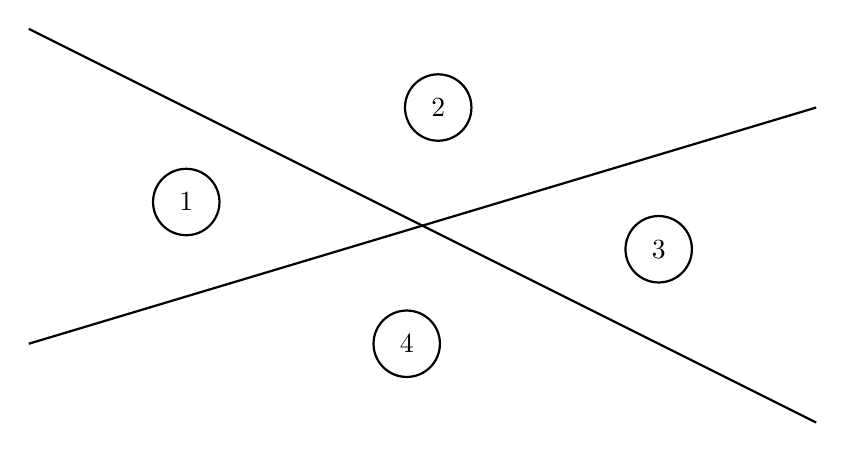
\begin{tikzpicture}[thick]
        \draw (-5,2.5) -- (5,-2.5);
        \draw (-5,-1.5) -- (5,1.5);
        \node[draw,circle,minimum size=24pt,inner sep=0,anchor=center] at (-0.2,-1.5) {$4$};
        \node[draw,circle,minimum size=24pt,inner sep=0,anchor=center] at (3,-0.3) {$3$};
        \node[draw,circle,minimum size=24pt,inner sep=0,anchor=center] at (-3,0.3) {$1$};
        \node[draw,circle,minimum size=24pt,inner sep=0,anchor=center] at (0.2,1.5) {$2$};
    \end{tikzpicture}
\end{center}

然而,这只是两条直线相交的\emph{特例}。如何证明\emph{任意}两条非平行直线\emph{总能}得到四个区域?也就是说,我们能否以某种方式结合直线数量 $n = 2$ 这一事实来描述这是\text{如何}发生的?思考一下!

下面是我们的方法。请注意,当我们添加第二条直线时,每个已经存在的区域都会被分成两部分,并且\emph{无论你如何绘制直线},只要确保两条直线不平行,结果都是这样。也就是说,如果我们用一条直线将平面分成两个区域,

\begin{center}
    \begin{tikzpicture}[thick]
        \draw (-5,2.5) -- (5,-2.5);
        \node[draw,circle,minimum size=24pt,inner sep=0,anchor=center] at (-3,0.3) {$1$};
        \node[draw,circle,minimum size=24pt,inner sep=0,anchor=center] at (0.2,1.5) {$2$};
    \end{tikzpicture}
\end{center}

然后添加一条新的直线会将每个现有区域分成两部分。这会向整个平面添加两个新的区域,总共四个区域:

\begin{center}
    \begin{tikzpicture}[thick]
        \draw (-5,2.5) -- (5,-2.5);
        \draw [color=red] (-5,-1.5) -- (0,0)  node[midway,below,sloped]{分割区域 1}
        -- (5,1.5) node[midway,above,sloped]{分割区域 2} ;
        \node[draw,circle,minimum size=24pt,inner sep=0,anchor=center,color=red] at (-0.2,-1.5) {$4$};
        \node[draw,circle,minimum size=24pt,inner sep=0,anchor=center,color=red] at (3,-0.3) {$3$};
        \node[draw,circle,minimum size=24pt,inner sep=0,anchor=center] at (-3,0.3) {$1$};
        \node[draw,circle,minimum size=24pt,inner sep=0,anchor=center] at (0.2,1.5) {$2$};
    \end{tikzpicture}
\end{center}

当 $n = 3$ 时呢?在这种情况下,我们需要考虑向具有两条直线和四个区域的图形中添加第三条直线。我们想要提出一个不依赖于线的特定排列的论证,因此我们最终唯一能用的事实是线之间互不平行,且任何交点仅位于两条线(而不是三条或更多)上。不过,就目前而言,查看特定的直线排列会有所启发,以便我们讨论相同的图形;我们可以利用对这个特定图形的观察来指导我们的一般论证。让我们从下方具有两条直线的图开始,向其中添加第三条直线,让第三条直线的交点都在初始交点``附近''或在图的范围内,这样我们就缩放图形了:

\begin{center}
    \begin{tikzpicture}[thick]
        \draw (-5,2.5) -- (5,-2.5);
        \draw (-5,-1.5) -- (5,1.5);
        \draw [color=red] (-5,1) -- (-1.8085,0.9043) node[midway,below,sloped]{\small 分割区域 1} 
        -- (2.5758,0.7727) node[midway,above,sloped]{\small 分割区域 2}
        -- (5,0.7) node[midway,below,sloped]{\small 分割区域 3};
        \node[draw,circle,minimum size=16pt,inner sep=0,anchor=center] at (-0.2,-1.5) {$4$};
        \node[draw,circle,minimum size=16pt,inner sep=0,anchor=center] at (3,-0.3) {$3$};
        \node[draw,circle,minimum size=16pt,inner sep=0,anchor=center] at (-3,-0.3) {$1$};
        \node[draw,circle,minimum size=16pt,inner sep=0,anchor=center] at (0.2,2) {$2$};
        \node[draw,circle,minimum size=16pt,inner sep=0,anchor=center,color=red] at (-4,1.45) {$5$};
        \node[draw,circle,minimum size=16pt,inner sep=0,anchor=center,color=red] at (0.1,0.45) {$6$};
        \node[draw,circle,minimum size=16pt,inner sep=0,anchor=center,color=red] at (4.61,1.05) {$7$};
    \end{tikzpicture}
\end{center}

很明显此时共有 $7$ 个区域。将第三条直线标绘为不同颜色,以便我们可以识别``新''区域出现的位置:一个区域(下方区域,区域 $4$)保持不变,但其他三个区域被一分为二,每次分割使区域计数加 $1$。如果我们以不同的方式绘制这条直线会怎样?

\begin{center}
    \begin{tikzpicture}[thick]
        \draw (-5,2.5) -- (5,-2.5);
        \draw (-5,-1.5) -- (5,1.5);
        \draw [color=red] (0,2.5) -- (-0.8333,0.4167) node[midway,right,sloped,rotate=-90]{\small 分割区域 2} 
        -- (-1.1364,-0.341) node[midway,left,sloped,rotate=-90]{\small 分割区域 1}
        -- (-2,-2.5) node[midway,right,sloped,rotate=-90]{\small 分割区域 4}; 
        \node[draw,circle,minimum size=16pt,inner sep=0,anchor=center] at (-0.2,-1) {$4$};
        \node[draw,circle,minimum size=16pt,inner sep=0,anchor=center] at (3,-0.3) {$3$};
        \node[draw,circle,minimum size=16pt,inner sep=0,anchor=center] at (-3,-0.3) {$1$};
        \node[draw,circle,minimum size=16pt,inner sep=0,anchor=center] at (1,2) {$2$};
        \node[draw,circle,minimum size=12pt,inner sep=0,anchor=center,color=red] at (-0.7,0.05) {$5$};
        \node[draw,circle,minimum size=16pt,inner sep=0,anchor=center,color=red] at (-1.5,1.8) {$6$};
        \node[draw,circle,minimum size=16pt,inner sep=0,anchor=center,color=red] at (-2.5,-1.4) {$7$};
    \end{tikzpicture}
\end{center}

类似的情况再次出现:其中一个区域保持不变,其余三个区域一分为二。(为何无其他区域?此问题值得深入思考。)尝试三条线的其他排列方式,并验证这种情况总会发生;此外,思考一下\emph{为什么}会出现这种情况,以及我们\emph{如何}解释这种情况一定会发生。不过,在给出一般性解释之前,我们再来看一下 $n=4$ 的情形。

当 $n = 4$ 时,我们从 $3$ 条直线和 $7$ 个区域的平面开始,添加第四条直线,该直线不与任何现有直线平行,并且不穿过任何现有交点。同样,我们想要提出一个与直线的特定排列无关的论证,但是查看下面的具体图形将有助于引导思路:

\begin{center}
    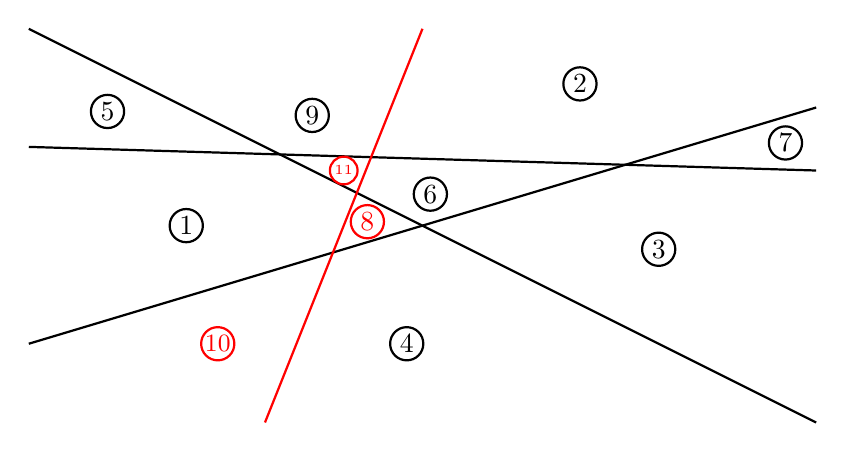
\begin{tikzpicture}[thick]
        \draw (-5,2.5) -- (5,-2.5);
        \draw (-5,-1.5) -- (5,1.5);
        \draw  (-5,1) -- (5,0.7);
        \draw [color=red] (0,2.5) -- (-2,-2.5);
        \node[draw,circle,minimum size=12pt,inner sep=0,anchor=center] at (-0.2,-1.5) {$4$};
        \node[draw,circle,minimum size=12pt,inner sep=0,anchor=center] at (3,-0.3) {$3$};
        \node[draw,circle,minimum size=12pt,inner sep=0,anchor=center] at (-3,0) {$1$};
        \node[draw,circle,minimum size=12pt,inner sep=0,anchor=center] at (2,1.8) {$2$};
        \node[draw,circle,minimum size=12pt,inner sep=0,anchor=center] at (-4,1.45) {$5$};
        \node[draw,circle,minimum size=12pt,inner sep=0,anchor=center] at (-1.4,1.4) {$9$};
        \node[draw,circle,minimum size=10pt,inner sep=0,anchor=center,color=red] at (-1,0.7) {\tiny $11$};
        \node[draw,circle,minimum size=12pt,inner sep=0,anchor=center] at (4.61,1.05) {$7$};
        \node[draw,circle,minimum size=12pt,inner sep=0,anchor=center,color=red] at (-0.7,0.05) {$8$};
        \node[draw,circle,minimum size=12pt,inner sep=0,anchor=center] at (0.1,0.4) {$6$};
        \node[draw,circle,minimum size=12pt,inner sep=0,anchor=center,color=red] at (-2.6,-1.5) {\small $10$};
    \end{tikzpicture}
\end{center}

请注意,三个原始区域保持不变(区域 $3$、区域 $5$ 和区域 $7$),而其他四个区域被一分为二。你注意到其中的规律了吗?对于每个已检验的 $n$,添加第 $n$ 条线会使 $n-1$ 个区域保持不变,其余区域则被一分为二。现在,让我们解释这一现象的原因。回忆一下,当绘制 $n$ 条直线时,我们的目标是确定区域的总数。为此,我们赋予该值一个名称以便引用:设 $R(n)$ 表示在平面上绘制 $n$ 条直线所创建的区域数,其中任意两条直线均不平行,且任意三条直线不共点。在上述示例中,我们考察了较小的 $n$ 值,并研究了添加新直线时的变化规律;也就是说,我们可以通过已知的 $R(n - 1)$ 推导 $R(n)$ 的值。现在,让我们将观察结果推广到适用于\emph{任意} $n$ 的情形。

假设已知 $R(n)$(为何可行?对于特定 $n$,我们是否确切知道 $R(n)$ 的值?它是什么?如何得知?)。考虑平面上满足题目条件的\emph{任意} $n$ 条直线图,这些直线将平面划分为 $R(n)$ 个区域。现在,添加第 $(n + 1)$ 条直线时会发生什么?关于这条直线如何改变图形,我们能确定哪些信息?关键约束如下:

\begin{enumerate}[label=(\alph*)]
    \item 新直线与现有的 $n$ 条直线均不平行;
    \item 新直线不经过任何现有交点。
\end{enumerate}

条件 (a) 表明新直线必与\emph{所有} $n$ 条已有直线相交(平行线无交点,非平行线必相交)。因此,新直线将产生 $n$ 个新交点。这些交点会与已有交点重合吗?不会!这正是条件 (b) 的作用。综上,只要满足题目要求,新直线上\emph{必定}存在 $n$ 个``特殊''点——即它与已有直线的交点。

接下来,我们利用这些特殊点识别新增区域。回顾之前的案例:标记新交点,并探究它们与新区域的关联。建议用圆点标记交点,并用 $\textbf{×}$ 标识新区域以增强可视性。下图展示了 $n = 4$ 的示例。你发现了什么?能否通过这些点推断添加第 $n$ 条直线后新增的区域数?思考一下,然后继续阅读。

\begin{center}
    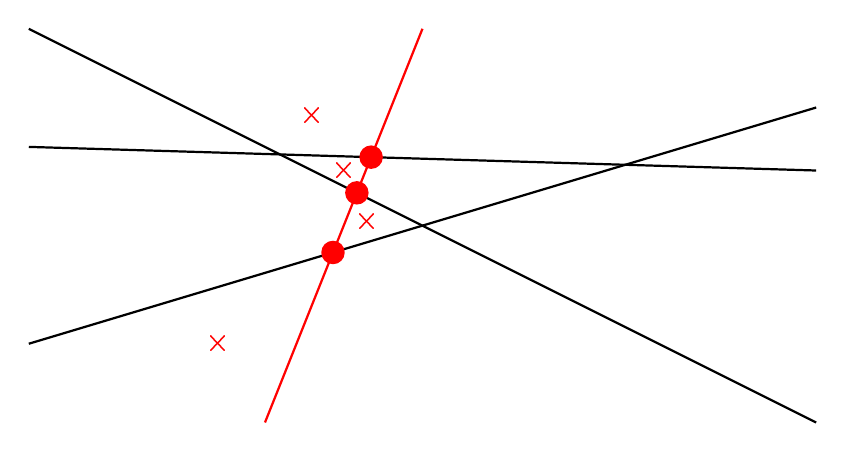
\begin{tikzpicture}[thick]
        \draw (-5,2.5) -- (5,-2.5);
        \draw (-5,-1.5) -- (5,1.5);
        \draw  (-5,1) -- (5,0.7);
        \draw [color=red] (0,2.5) -- (-2,-2.5);
        \node[minimum size=14pt,anchor=center,color=red,very thick] at (-1.4,1.4) {$\textbf{×}$};
        \node[minimum size=14pt,anchor=center,color=red,very thick] at (-1,0.7) {$\textbf{×}$};
        \node[minimum size=14pt,anchor=center,color=red,very thick] at (-0.7,0.05) {$\textbf{×}$};
        \node[minimum size=14pt,anchor=center,color=red,very thick] at (-2.6,-1.5) {$\textbf{×}$};
        \node[fill,circle,inner sep=3pt,color=red] at (-0.6522,0.8696) {};
        \node[fill,circle,inner sep=3pt,color=red] at (-0.8333,0.4167) {};
        \node[fill,circle,inner sep=3pt,color=red] at (-1.1364,-0.341) {};
    \end{tikzpicture}
\end{center}

没错!任意两个相邻新交点之间,都有一条\emph{线段}恰好将一个区域一分为二!接下来只需确定此类线段的数量即可。由于每条线段仅分割\emph{一个}已有区域,其数量即等于新增区域数。已知第 $(n + 1)$ 条直线产生 $n$ 个新交点。这些点在直线上如何排列?任意两个``连续'交点形成一条有限线段,而端点则延伸为无限射线(经端点无限延伸)。总计多少条线段?恰好 $n + 1$ 条(参考 $n = 3$ 的示意图:$3$ 个交点对应 $4$ 条线段,含两条无限射线)。因此,$n + 1$ 条线段分割出 $n + 1$ 个新区域,即:
\[R(n + 1) = R(n) + n + 1\]
出色的发现!通过分析示例和几何论证,我们成功揭示了递归关系:$R(n+1)$ 的值依赖于 $R(n)$。虽未完全解决问题,但已接近目标。接下来只需迭代展开 $R(n)$ 的表达式,直至已知的 $R(1) = 2$。过程如下:

\begin{center}
    \begin{tabular}{rcccccccccc}
        $R(n+1)$ & $=$ &          & &            &     &            &     & $\cancel{R(n-1)}$ & $+$ & $n+1$\\
                 & $=$ &          & &                   &     & $\cancel{R(n-1)}$ & $+$ & $n$ & $+$ & $n+1$\\
                 & $=$ &          & & $\cancel{R(n-2)}$ & $+$ & $(n-1)$           & $+$ & $n$ & $+$ & $n+1$\\
                 & $\vdots$ &     & &  &  &  &  &  &  & \\
                 & $=$ &          & & $\cancel{R(2)}+3$ & $+$ & $\dots$ & $+$ & $n$ & $+$ & $n+1$ \\
                 & $=$ & $R(1)+2$ & $+$ & $3$               & $+$ & $\dots$ & $+$ & $n$ & $+$ & $n+1$ \\
    \end{tabular}
\end{center}

由 $R(1) = 2$ 可得:
\[R(n + 1) = 2 + \left(2 + 3 + \dots + n + (n + 1)\right) = 2 + \left(\sum_{k=1}^{n+1}k\right)-1 = 1+\sum_{k=1}^{n+1}k\]
而这正是我们之前研究过的求和公式!(注意括号内求和缺首项 $k=1$,故需减去 $1$)。回忆 $\sum_{k=1}^{n} k = \frac{n(n+1)}{2}$,为了表示上面等式中的求和,我们只需将 $n$ 替换为 $n + 1$ 即可。因此,
\[R(n + 1) = 1+\frac{(n+1)(n+2)}{2}\]
最后,为得到 $R(n)$ 的显式表达式,将 $n+1$ 替换为 $n$(对 $n$ 的取值有什么要求?):
\[R(n + 1) = 1+\frac{n(n+1)}{2}\]
至此,我们获得了原问题的答案!此过程运用了\emph{归纳}技术:通过建立 $R(n + 1)$ 对 $R(n)$ 的依赖关系,反向迭代至\emph{已知}值 $R(1)$。

需要强调的是,本节推导旨在引导直觉而非提供\emph{严格证明}。省略号(``$\dots$'')并非严谨的数学归纳表述。此外,我们的方法是从 $n - 1$ 条直线出发\emph{逐步构建} $n$ 条直线的情形——这是否合理?为何能推广到 $n$ 条直线的\emph{任意}图?所有此类图是否均来自少一条线的子图?

接下来的两章将引入严格工具以形式化上述方法,并建立数学归纳的严谨框架。当前阶段,我们仅提供归纳法的启发式定义,并继续探索依赖归纳的有趣问题。重点在于练习识别归纳结构、运用其解决问题等技能,这对未来学习至关重要(暂无需深入数学细节!)。


% !TeX root = ../../../book.tex
\subsection{习题}

\subsubsection*{温故知新}

以口头或书面的形式简要回答以下问题。这些问题全都基于你刚刚阅读的内容,所以如果忘记了具体的定义、概念或示例,可以回去重读相关部分。确保在继续学习之前能够自信地回答这些问题,这将有助于你的理解和记忆!

\begin{enumerate}[label=(\arabic*)]
    \item 归纳过程有哪些特征?
    \item 我们如何证明 $\sum_{k=1}^{n}k = \frac{n(n+1)}{2}$ 是正确的?我们的方法是如何归纳的?(如果你不记得了,请重读第 \ref{sec:section1.4.2} 节!)
    \item 为什么我们可以把上一个问题中提到的求和公式,用 $n+1$ ``替换'' $n$,并且知道它仍然成立?我们也可以将 $n$ 替换为 $n - 1$ 吗?
    \item 通过代数步骤获得前 $n$ 个自然数平方和的最终表达式;也就是说,验证
    \[\frac{1}{3}(n+1)^3-\frac{1}{3}(n+1)-\frac{n(n+1)}{2} = \frac{1}{6}n(n+1)(2n+1)\]
    \item 试着回忆一下向平面中添加第 $(n+1)$ 条直线正好会创建 $n+1$ 个新区域的论点。你能为朋友证明这个论点并说服他/她它是有效的吗?
    \item 求前 $n$ 个自然数的平方和,为什么不能把前 $n$ 个自然数之和的公式平方呢?为什么这是错误的?
\end{enumerate}

\subsubsection*{小试牛刀}

尝试回答以下问题。这些题目要求你实际动笔写下答案,或(对朋友/同学)口头陈述答案。目的是帮助你练习使用新的概念、定义和符号。题目都比较简单,确保能够解决这些问题将对你大有帮助!

\begin{enumerate}[label=(\arabic*)]
    \item 在平面中画 $5$ 条直线(满足原题的两个条件)并验证是否有 $16$ 个区域。你还能验证 $6$ 条线产生 $22$ 个区域吗?
    \item 给出序列 $1, 2, 3, 4, \dots , 100$ 的另一种解释,而不仅仅是从 $1$ 到 $100$ 的所有自然数。(回想一下我们给出的例子:$1$ 到 $100$ 之间所有英文拼写中不含字母"i"的数字。)
    \item 提出一个将 $(n + 1)^4$ 与 $n^4$ 联系起来的代数表达式,就像我们对立方所做的那样。\\ 
    (\textbf{挑战题:}你能为刚刚推导出的表达式给出\emph{几何}解释吗?)
    \item \textbf{挑战题:}让我们将``平面上的线''这题提升一个维度!考虑三维空间中有 $n$ 个平面。会创建多少个区域?假设没有两个平面平行,并且没有三个或以上平面相交于一条直线。(想想这两个条件如何直接类比于``线''那题的给定条件。)
\end{enumerate}

\newpage
% !TeX root = ../../../book.tex
\section{定义归纳}

为了将数学归纳法定义为证明技术,我们想强调,上一节中的例子使用了问题结构的某些直观概念来给出问题的``解'',我们在\emph{解}上加了引号,表明我们还没有正式证明它。从这个意义上讲,我们提出以下问题:如果\emph{给定}我们前面推导的公式并要求验证它怎么办?如果我们没有通过任何直观的步骤来推导公式,只是有人告诉我们它是正确的怎么办?我们如何验证他们的说法?之所以问这个问题,是因为我们现在确实面临着这种情况,除非告诉我们公式的人采用与我们相同的直觉论证。

假如一个持怀疑态度的朋友说:``嘿,我听说过一个计算前 $n$ 个自然数平方和的公式。有人告诉我,它们加起来等于 $\frac{1}{6}n(n+1)(2n+1)$。我验证了前两个自然数,全都正确,所以它一定是正确的。应该传播出去!'' 作为一个理性思考者,同时也是好朋友的身份,你点点头说:``我确实听说了,但让我们确保这个公式对每个数字都是正确的。'' 你将如何进行?你的朋友说的没错,前几个值确实``完美匹配'':

\begin{align*}
    1^2 &= \enspace 1 = \frac{1}{6}(1)(2)(3) \\
    1^2 + 2^2 &= \enspace 5 = \frac{1}{6}(2)(3)(5) \\
    1^2 + 2^2 + 3^2 &= 14 = \frac{1}{6}(3)(4)(7) \\
    1^2 + 2^2 + 3^2 + 4^2 &= 30 = \frac{1}{6}(4)(5)(9)
\end{align*}
如果我们愿意的话,我们甚至可以手动检验 $n$ 的更大的值:
\[1^2 + 2^2 + 3^2 + 4^2 + 5^2 + 6^2 + 7^2 + 8^2 + 9^2 + 10^2 = 385 = \frac{1}{6}(10)(11)(21)\]
但请记住,该公式声称对于\emph{任意} $n$ 值都有效。手动检验每个结果将花费大量时间,因为自然数有\emph{无穷}多个。无论我们检验多少个独立的 $n$ 值,总会有更大的值,我们怎么\emph{知道}公式对于某些大值不会失效?从数学和时间上来讲,我们需要一个更加\emph{有效}的方法,以某种方式只需几步即可验证所有 $n$ 值。我们先在心里埋下一颗种子(这是即将推出的数学归纳法的严格版本),在这里我们将从广义上解释该过程是如何工作的。

% !TeX root = ../../../book.tex
\subsection{多米诺骨牌类比}

假设我们有一副特殊的多米诺骨牌,它包含无穷多张骨牌!每张骨牌可以书写任意内容,而非标准的点数。这些骨牌沿无限延伸的桌面排列成无限长的一行。从侧面观察时,每张骨牌下方标有位置标签:

\begin{center}
    \begin{tikzpicture}
        \foreach \x in {1,...,5}
        {
            \pic [fill=white] at (\x, 0, 0) {annotated cuboid={width=3, height=30, depth=10}};
            \node[below] at (\x, -3){\tiny $n=\x$};
        }
        \node[anchor=center] at (6.5, -1.5){\LARGE $\dots \cdot$};
        % \pic [very thick,densely dashed,draw=blue] at (5,0) {annotated cuboid={width=30, height=5, depth=10, opacity=0.2}};
    \end{tikzpicture}
\end{center}

对于这个特定的例子,我们需要验证公式
\[\sum_{k=1}^{n}k^2 = \frac{1}{6}n(n+1)(2n+1)\]
为此,设想每张多米诺骨牌记载一个特定``事实''。具体来说,我们可以想象第一张多米诺骨牌上写有表达式
\[\sum_{k=1}^{1}k^2 = \frac{1}{6}(1)(1)(3)\]
第二张多米诺骨牌上写有表达式
\[\sum_{k=1}^{2}k^2 = \frac{1}{6}(2)(3)(5)\]
推而广之,第 $n$ 张骨牌写有如下``事实'':
\[\sum_{k=1}^{n}k^2 = \frac{1}{6}n(n+1)(2n+1)\]
由于多米诺骨牌具有连锁倾倒的特性,我们约定骨牌倒下即表示其记载的``事实''是\emph{真实命题}。由此将多米诺骨牌的物理解释与公式有效性的数学解释联系起来。

我们已手动验证 $n=1$ 的情形:$1^2=\frac{1}{6}(1)(2)(3)$,故第一张骨牌记载的命题为真,必将倒下。同理验证 $n=2$ 后,第二张骨牌也会倒下:

\begin{center}
    \begin{tikzpicture}
        \foreach \x in {1,2}
        {
            \pic [fill=white, rotate=-30, anchor=south] at (\x, -0.15, 0) {annotated cuboid={width=3, height=32, depth=10}};
            \node[below] at (\x-1.5, -3){\tiny $n=\x$};
        }
        \foreach \x in {3,4,5}
        {
            \pic [fill=white] at (\x, 0, 0) {annotated cuboid={width=3, height=30, depth=10}};
            \node[below] at (\x, -3){\tiny $n=\x$};
        }
        \node[anchor=center] at (6.5, -1.5){\LARGE $\dots \cdot$};
        % \pic [very thick,densely dashed,draw=blue] at (5,0) {annotated cuboid={width=30, height=5, depth=10, opacity=0.2}};
    \end{tikzpicture}
\end{center}
然而,若继续逐个检验,又会陷入原先的困境——我们不可能验证\emph{每张}骨牌。真正的需求是捕捉多米诺效应的精髓:一张骨牌倒下将触发下一张倒下。这要求我们建立相邻骨牌所载``事实''的数学关联。

让我们看看前两张多米诺骨牌的情况。既然知道骨牌 $1$ 倒下,我们能否在不重写所有求和项的情况下确保骨牌 $2$ 倒下?两块骨牌上的陈述有何关联?每个陈述都是自然数的平方和,且第二张骨牌的陈述正好多出一项。因此,利用骨牌 $1$ 上已知的\emph{真实陈述},可以\emph{验证}骨牌 $2$ 上陈述的真实性:
\[\sum_{k=1}^{2}k^2 = 1^2+2^2=1+2^2=5=\frac{1}{6}(2)(3)(5)\]
尽管节省的唯一``工作''只是免于计算 $1^2=1$,但让我们在更大数字上应用此过程以凸显其优势。\emph{假设}骨牌 $10$ 已经倒下(其求和的完整验证已在前文给出),这意味着我们\emph{知道}
\[\sum_{k=1}^{10}k^2 =\frac{1}{6}(10)(11)(21)=285\]
是一个\emph{真实陈述}。利用它来验证骨牌 $11$ 的陈述:
\[\sum_{k=1}^{11}k^2 =\frac{1}{6}(11)(12)(23)\]
骨牌 $11$ 上的求和公式有 $11$ 项,前 $10$ 项正是骨牌 $10$ 上的求和!因此只需分离第 $11$ 项并代入已知结果:
\begin{align*}
    \sum_{k=1}^{11}k^2 &= (1^2+2^2+\dots+10^2)+11^2\\
    &=\sum_{k=1}^{10}k^2+11^2\\
    &=385+121\\
    &=506\\
    &=\frac{1}{6}3036=\frac{1}{6}(11)(12)(23)
\end{align*}
节省的工作量显而易见!既然已知前 $10$ 项之和,何必重新计算?

现在设想对\emph{所有} $n$ 值\emph{同时}实施此过程!若能证明每当骨牌 $n$ 倒下,骨牌 $(n + 1)$ \emph{必然}倒下,这意味着什么?回顾无穷骨牌序列:已知骨牌 $1$ 因手动检验而倒下,加之``骨牌 $n$ 撞倒骨牌 $(n + 1)$''的普适性验证,可推得骨牌 $1$ 撞倒骨牌 $2$,骨牌 $2$ 撞倒骨牌 $3$,骨牌 $3$ 撞倒骨牌 $4$,…… 如此传递下去,整列骨牌终将全部倒下!本质上,整个过程可归结为\emph{两步}:

\begin{enumerate}[label=(\arabic*)]
    \item 确保第一张骨牌倒下;
    \item 确保每张骨牌都能撞倒下一张骨牌。
\end{enumerate}
仅凭这两步,便能\emph{保证}所有骨牌倒下,从而\emph{证明}每个公式对\emph{任意}自然数 $n$ 成立。

我们已经完成步骤 (a),现在需要完成步骤 (b)。此前已针对特定案例(骨牌 $1$ 撞倒骨牌 $2$、骨牌 $10$ 撞倒骨牌 $11$)执行了此操作,现在将其推广到任意 $n$ 值。我们\emph{假设}:对于某个\emph{特定}但\emph{任意}的 $n$,多米诺骨牌 $n$ 会倒下,这意味着方程
\[\sum_{k=1}^{n}k^2=\frac{1}{6}n(n+1)(2n+1)\]
为\emph{真实陈述}。现在需将其关联到骨牌 $(n+1)$ 的陈述,并应用上述等式信息。将 $n+1$ 项的和拆分为 $n$ 项和与末项:
\[\sum_{k=1}^{n+1}k^2 = (1^2+2^2+\dots+n^2+(n+1)^2)=\sum_{k=1}^{n}k^2+(n+1)^2\]
根据骨牌 $n$ 倒下的假设(即其命题为真),可得
\[\sum_{k=1}^{n+1}k^2 = \frac{1}{6}n(n+1)(2n+1)+(n+1)^2\]
这与骨牌 $(n+1)$ 的命题是否一致?骨牌 $(n+1)$ 的``事实''与骨牌 $n$ 类似,只是将``$n$''替换为``$n + 1$'':
\[\sum_{k=1}^{n+1}k^2 = \frac{1}{6}\big(n+1\big)\big((n+1)+1\big)\big((2(n+1)+1)\big)=\frac{1}{6}(n+1)(n+1)(2n+3)\]
目前还不清楚我们推导出的表达式是否实际上等于上面的式子。我们可以尝试化简该表达式,并将其分解为与上面表达式``类似''的新表达式,但展开两个表达式并比较所有项可能会更容易。(这基于这样的一般思想:展开因式分解后的多项式比进行因式分解要容易得多。)对于第一个表达式,我们有
\begin{align*}
    \frac{1}{6}n(n + 1)(2n + 1) + (n + 1)^2 &=\frac{1}{6}n(2n^2 + 3n + 1) + (n^2 + 2n + 1)\\
    &= \frac{1}{3}n^3 + \frac{1}{2}n^2 + \frac{1}{6}n + n^2 + 2n + 1 \\
    &= \frac{1}{3}n^3 + \frac{3}{2}n^2 + \frac{13}{6}n + 1
\end{align*}
对于第二个表达式,我们有
\begin{align*}
    \frac{1}{6}(n+1)(n + 2)(2n + 3) &=\frac{1}{6}(n+1)(2n^2 + 7n+6)\\
    &= \frac{1}{6}\big[(2n^3 + 7n^2 + 6n) + (2n^2 + 7n + 6)\big] \\
    &= \frac{1}{3}n^3 + \frac{3}{2}n^2 + \frac{13}{6}n + 1
\end{align*}
可见两式相等!此外,请注意,这比尝试整理其中一个表达式并将其``变形''为另一个表达式要容易得多。我们通过展开两式并最终得到相同的表达来证明它们是相同的。现在,让我们回顾并总结我们所取得的成果:
\begin{enumerate}
    \item 我们将证明公式
    \[\sum_{k=1}^{n+1}k^2 = \frac{1}{6}n(n+1)(2n+1)+(n+1)^2\]
    对于\emph{所有} $n$ 值成立类比为推倒无穷多的多米诺骨牌。
    \item 通过手工计算验证骨牌 $1$ 的命题成立,骨牌 $1$ 倒下;
    \item \emph{假设}骨牌 $n$ 的命题为真,由骨牌 $n$ 命题成立推出骨牌 $(n+1)$ 命题成立,从而证明骨牌 $n$ 会撞倒骨牌 $(n+1)$。
    \item 由此保证所有骨牌都会倒下,因此公式对\emph{所有} $n$ 都成立。
\end{enumerate}
此方法是否严谨?是否已\emph{严格证明}公式对所有自然数 $n$ 都成立?若存在 $n$ 使得公式失效,这对多米诺骨牌体系意味着什么?

请记住,这里的多米诺骨牌类比只是理解归纳法工作原理的一个直观指引,并非建立在严格的数学基础之上。建立严格的数学基础将是接下来几章的目标。现在,让我们回顾本章讨论的另一个例子:直线划分平面区域。同样,在推导公式 $R(n)$ 时使用省略号显得繁琐,我们希望避免这种做法。让我们尝试将多米诺骨牌类比应用于此问题。

设想我们定义 $R(n)$ 为 $n$ 条直线在平面上划分出的不同区域的数量,这些直线满足互不平行且任意三条(或更多)直线不共点。进一步设想,我们在代表第 $n$ 步的骨牌上写下``$R(n) = 1 + \frac{n(n+1)}{2}$''这一``事实''。能否按照与之前相同的逻辑来验证所有骨牌都会倒下?

首先,需要验证骨牌 $1$ 是否会倒下。这等同于验证命题``$R(1) = 1+\frac{1(2)}{2} = 1+1 = 2$''是否成立。这显然成立,正如我们之前验证过的:一条直线将平面划分为两个区域。其次,需要证明对于\emph{任意} $n$,第 $n$ 块骨牌倒下必定导致第 $(n + 1)$ 块骨牌倒下。也就是说,我们\emph{假设}``$R(n) = 1 + \frac{n(n+1)}{2}$''对某个特定的 $n$ 成立,然后\emph{证明}``$R(n + 1) = 1 + \frac{(n+1)(n +2)}{2}$''也必然成立。如何证明?沿用之前的思路,建立 $R(n + 1)$ 与 $R(n)$ 的关系。向\emph{任意}满足条件的 $n$ 条直线的图形中添加一条新直线,通过几何分析,我们得到关系式 $R(n+1) = R(n) + n + 1$。利用此关系以及第 $n$ 块骨牌倒下的假设,可得:
\[R(n + 1) = R(n) + n + 1 = 1 +\frac{n(n+1)}{2}+ n + 1\]
这个结果是否与骨牌 $(n + 1)$ 上的表达式一致?通过化简比较即可验证:
\[1 +\frac{n(n+1)}{2}+ n + 1=2+n+\frac{n^2+n}{2} = \frac{1}{2}n^2+\frac{3}{2}n+2\]
以及
\[1 + \frac{(n+1)(n +2)}{2} = 1+\frac{n^2+3n+2}{2} =  \frac{1}{2}n^2+\frac{3}{2}n+2\]
结果完全相同!因此,我们证明了对于\emph{任意} $n$,骨牌 $n$ 倒下\emph{必然}导致骨牌 $(n+1)$ 倒下。

思考一下,使用这种``多米诺骨牌技术''进行的证明,与我们之前为推导该公式所采用的方法有何不同?我们在本节中是否使用了省略号?为何这种证明方式更优?我们是否曾用多米诺骨牌归纳技术来推导公式本身?


% !TeX root = ../../../book.tex
\subsection{其他类比}

多米诺骨牌类比非常流行,但它并不是归纳法工作方式的唯一描述。根据你的阅读内容或交谈对象,可能会学到不同的类比,或其他类型的描述。这里,我们将描述以前听说过的两个。思考这些类比本质上的等价性,这将有助于巩固你对归纳法的理解(至少就我们所开发的而言)。

\subsubsection*{神奇的数学猴子 Mojo}

想象一个无穷天梯,直矗云霄。梯子有无数级,按 $1, 2, 3$ 的顺序依次编号。我们的朋友 Mojo 恰好站在梯子旁。他是一只聪明的猴子,对数学很感兴趣,但也有点神奇,因为他真的可以爬上这个无穷天梯!

如果 Mojo 到达了阶梯上的某一级,则意味着与该数字对应的事实为真。我们怎样才能确保他爬完整个梯子?单独检查每个阶梯的效率很低。想象一下:我们必须站在地面上确保他到达第 $1$ 级,然后我们必须稍微抬起头来确保他到达了第 $2$ 级,然后是第 $3$ 级,依此类推……相反,我们在 Mojo 开始攀爬之前确认了两个细节。他要开始攀爬了吗?也就是说,他会爬上第 $1$ 级吗?如果是这样,那就太好了!另外,阶梯之间的距离是否足够近,以便无论他在哪里,\emph{总能}到达下一个阶梯?如果是这样,那就更棒了!这些与我们在多米诺骨牌类比中建立的条件完全相同。为了确保 Mojo 到达\emph{每个}阶梯,我们只需要知道他到达了第 $1$ 个阶梯,并且他总是可以到达下一个阶梯。

\subsubsection*{归纳鸭 Doug}

再来认识一下 Doug。他是一只鸭子。他喜欢面包,所以他会去每个人的院子里寻找更多的面包。这些院子都沿数学镇的归纳街而建,房子的编号是 $1, 2, 3, \dots$ 以此类推。

Doug 从 $1$ 号院子开始寻找面包。没有找到任何东西,所以他依旧很饿。还能去哪里找?隔壁还有 $2$ 号院子!Doug 朝那边走去,肚子咕咕叫。他在那里也没找到面包,所以他必须继续寻找。此时他已经知道 $1$ 号院子没有面包,所以唯一去向就是隔壁的 $3$ 号院子。我想你已经明白事情的发展方向了…… 

如果我们跟踪 Doug 的进展,我们可能想知道他最终是否到达了每一个院子。假设我们已经提前知道\emph{没人}有面包。这意味着,每当 Doug 在某个院子里时,他一定会去隔壁院子,继续寻找食物。这意味着他一定会挨家挨户地去寻找!也就是说,无论我们住在哪栋房子里,无论我们门前的数字多大,在某个时点我们一定会看到 Doug 在我们的后院闲逛。(不幸的是,他会一直饿着肚子!可怜的 Doug。)


% !TeX root = ../../../book.tex
\subsection{总结}

回顾前两个示例的工作及我们的类比,可以发现每个问题都具有特定的\emph{结构}:某个``事实''依赖于``前一个事实''。对于立方数,我们找到了用 $n^3$ 表示 $(n + 1)^3$ 的方法;对于平面分割问题,我们刻画了向 $n$ 条直线的图形添加新直线时新增的区域个数。基于这些观察,我们反复应用已知关系,直至抵达一个可验证的``基础事实''——通常对应较小的 $n$ 值(两例中均为 $n = 1$)。这一过程使我们能够推导出适用于\emph{任意} $n$ 的通用公式或表达式。

尽管这项工作对公式推导至关重要且富有启发性,但它本身\emph{不足以证明}公式的有效性。在进行上述工作时,我们发现了归纳过程的存在,并利用其结构推导了相关表达式。这实际上有两个好处:不仅发现了待证公式,还让我们意识到采用\emph{数学归纳法}进行严格证明的可行性。

实际的``归纳证明''包含两个核心步骤:首先,验证公式在某个``起始值''成立;其次,\emph{假设}公式对某个特定 $n$ 成立,并以此证明其对 $n + 1$ 必然成立。完成这两步后,我们即可断言``所有多米诺骨牌都会倒下''——公式对所有相关 $n$ 值都成立。

\subsubsection*{一个问题:梯子的``尽头''是什么?}

你可能仍存疑虑,我们尝试在此预测你的担忧。(之所以提及这一点,是因为这是一个常见疑问。若你\emph{未曾}考虑这一点,请试着想象其来源。)你或许会说:``等等,现在我明白 Mojo 如何攀登天梯了,但他如何真正\emph{抵达顶端}呢?这是个无穷阶梯,对吗?那他永远无法到达终点……不是吗?''

某种意义上,你是对的。既然这个神奇阶梯将\emph{永远}延伸,它便没有真正的终点,Mojo 永无法抵达``顶端''。然而,这并非关键;我们不在意任何``\emph{顶端}''(不仅仅是因为\emph{不存在}顶端),只需确认 Mojo 能踏足\emph{每一个}台阶。他不必凌驾所有台阶立于顶端俯视来路——那不是目的!知道 Mojo 实际上到达了\emph{每一个可能的}阶梯。他不必超越所有人,站在梯子的顶端,俯视自己的来路。那不是目标!

不妨这样思考:假设你对某个待证事实抱有浓厚兴趣,例如
\[\text{事实\ } \#18,458,789,572,311,000,574,003 \text{\ (具体数值无关紧要)}\]
它对应遥不可及的台阶,而你只关心 Mojo 能否抵达。他会到达吗?他当然会!这或许需要漫长的时光(多少步呢?),但这在猴子与梯子的神奇世界,谁又在乎时间呢?你知道他终将抵达,这就够了。试想每个事实在神奇世界里都有专属关注者,每位关注着都将因 Mojo 踏足其关切之阶而欣喜。无人在意他能否登顶——那并非焦点。与此同时,在现实世界中,我们因\emph{所有}关注者终将如愿而欣慰。无限攀登的过程被简化为两步:仅凭此两步,我们便确信阶梯的\emph{每一级}皆可达,每个编号的事实皆成立。

亦可类比多米诺骨牌:我们是否在意骨牌链存在``终点'',最终撞上墙壁?当然不。骨牌链将永续延伸,每张牌终会倒下,时间长短无关紧要。同理,我们知晓 Doug 终将抵达\emph{所有}院子——何时抵达\emph{某个}院子无关紧要,唯有抵达\emph{全部}院子方为关键。


% !TeX root = ../../../book.tex
\subsection{习题}\label{sec:section2.3.4}

\subsubsection*{温故知新}

以口头或书面的形式简要回答以下问题。这些问题全都基于你刚刚阅读的内容,如果忘记了具体定义、概念或示例,可以回顾相关内容。确保在继续学习之前能够自信地作答这些问题,这将有助于你的理解和记忆!

\begin{enumerate}[label=(\arabic*)]
    \item 多米诺骨牌、Mojo 和 Doug 的类比为何等价?能否定义一个``函数''来描述它们之间的关系,实现类比间的相互转换?
    \item 找一位未接触过数学归纳法的朋友,尝试向他解释这一概念。你是否在解释中使用了上述类比?这些类比是否有帮助?
    \item 为什么我们对立方体的研究不足以证明求和公式?为何仍需完成后续推导?
    \item 思考多米诺骨牌的类比:若骨牌无限延伸是否会导致某些骨牌永不倒下?尝试用类比解释这一现象的含义。
\end{enumerate}

\subsubsection*{小试牛刀}

尝试解答以下问题。这些题目需动笔书写或口头阐述答案,旨在帮助你熟练运用新概念、定义及符号。题目难度适中,确保掌握它们将大有裨益!

\begin{enumerate}[label=(\arabic*)]
    \item 用数学归纳法证明公式:
    \[\sum_{k=1}^{n}k = \frac{n(n+1)}{2}\]
    \item 用数学归纳法证明公式:
    \[\sum_{k=1}^{n}2k-1 = n^2\]
    \item 用数学归纳法证明公式:
    \[\sum_{k=1}^{n}k^3 = \Bigg(\frac{n(n+1)}{2}\Bigg)^2\]
    \item 设存在一系列由自然数索引的命题,用``$P(n)$''表示第 $n$ 个命题。
    \begin{enumerate}[label=(\alph*)]
        \item 若要证明对所有自然数 $n$,\emph{每个} $P(n)$ 均成立,应该如何操作?
        \item 若只需证明当 $n$ 为\emph{偶数}时 $P(n)$ 成立,应该如何处理?能否通过修改某个类比来描述此方法?
        \item 若只需证明当 $n \geq 4$ 时 $P(n)$ 成立,又该如何处理?能否通过修改某个类比来描述此方法?
    \end{enumerate}
\end{enumerate}


\newpage
% !TeX root = ../../../book.tex
\section{另外两个(不同的)例子} \label{sec:section2.4}

本节有两个主要目的。首先,我们旨在避免读者产生归纳法仅适用于证明\emph{数值公式}(如涉及数字或多项式)的误解。归纳法的应用远比这广泛得多!特别是接下来的例子将证明:某些抽象性质对于给定情境中的任意``规模''均成立。我们会看到这仍属于``归纳''的范畴,同时也能观察到其与先前例子的区别。此外,这些例子还揭示了一个重要现象:有时推动多米诺骨牌需要掌握``更多信息''。在之前的案例中,仅需确认骨牌 $n$ 倒下,即可\emph{确保}骨牌 $n + 1$ 随之倒下。但在本节的示例中,我们可能需要了解前几个骨牌的状态。通过这两个例子,我们将总结其与前述多米诺骨牌模型的差异,并预览适用于此类情况的、更通用的归纳技术定义。

% !TeX root = ../../../book.tex
\subsection{多米诺与密铺} \label{sec:section2.4.1}

下面的示例比前两个示例稍微复杂一些。我们最终仍将证明某个数值公式,但问题显然比仅仅操纵代数表达式更加直观。此外,我们会在开始步骤中注意到一个有趣的``问题'',即我们必须解决几个``小案例'',然后才能推广我们的方法。这将是我们首次考虑如何泛化归纳技术使其适应其他情况。

我们要回答的问题可以表述如下:

\begin{quote}
    给定一个 $2 \times n$ 的正方形棋盘,有多少种不同的方式可以用多米诺骨牌平铺该棋盘?平铺必须让每个正方形都被一块——且只有一块——多米诺骨牌覆盖。
\end{quote}
例如,以下是正确的密铺

\begin{center}
    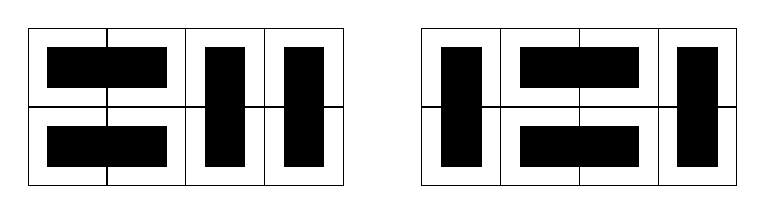
\begin{tikzpicture}[x=1.0cm, y=1.0cm]
        \foreach \y in {0,1} {
            \foreach \x in {0,...,3} {
                \draw (0+\x ,0+\y) rectangle ++ (1,1);
            }
        }

        \draw[fill, black] (0.25 ,0.25) rectangle ++ (1.5,0.5);
        \draw[fill, black] (0.25 ,1.25) rectangle ++ (1.5,0.5);
        \draw[fill, black] (2.25 ,0.25) rectangle ++ (0.5,1.5);
        \draw[fill, black] (3.25 ,0.25) rectangle ++ (0.5,1.5);

        \foreach \y in {0,1} {
            \foreach \x in {0,...,3} {
                \draw (5+\x ,0+\y) rectangle ++ (1,1);
            }
        }

        \draw[fill, black] (5+1.25 ,0.25) rectangle ++ (1.5,0.5);
        \draw[fill, black] (5+1.25 ,1.25) rectangle ++ (1.5,0.5);
        \draw[fill, black] (5+0.25 ,0.25) rectangle ++ (0.5,1.5);
        \draw[fill, black] (5+3.25 ,0.25) rectangle ++ (0.5,1.5);
    \end{tikzpicture}
\end{center}
而以下\emph{不}是正确的密铺

\begin{center}
    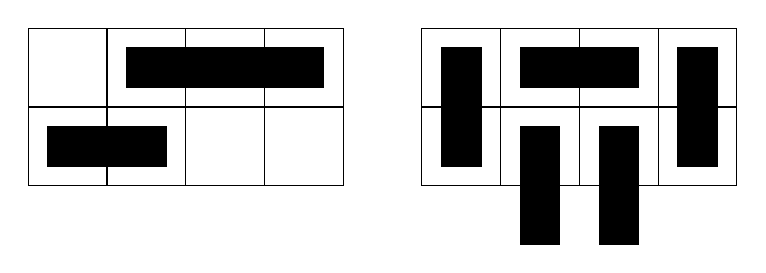
\begin{tikzpicture}[x=1.0cm, y=1.0cm]
        \foreach \y in {0,1} {
            \foreach \x in {0,...,3} {
                \draw (0+\x ,0+\y) rectangle ++ (1,1);
            }
        }

        \draw[fill, black] (0.25 ,0.25) rectangle ++ (1.5,0.5);
        \draw[fill, black] (1.25 ,1.25) rectangle ++ (1.5,0.5);
        \draw[fill, black] (2.25 ,1.25) rectangle ++ (1.5,0.5);

        \foreach \y in {0,1} {
            \foreach \x in {0,...,3} {
                \draw (5+\x ,0+\y) rectangle ++ (1,1);
            }
        }

        \draw[fill, black] (5+1.25 ,1.25) rectangle ++ (1.5,0.5);
        \draw[fill, black] (5+1.25 ,-0.75) rectangle ++ (0.5,1.5);
        \draw[fill, black] (5+2.25 ,-0.75) rectangle ++ (0.5,1.5);
        \draw[fill, black] (5+0.25 ,0.25) rectangle ++ (0.5,1.5);
        \draw[fill, black] (5+3.25 ,0.25) rectangle ++ (0.5,1.5);
    \end{tikzpicture}
\end{center}

和以前一样,让我们查看前几种情况(其中 $n = 1, 2, 3$ 等),看看我们是否能发现任何模式。在继续阅读之前,尝试自己解决该问题!

当 $n = 1$ 时,我们有一个与多米诺骨牌形状完全相同的棋盘,因此肯定只有一种方法可以密铺。让我们使用符号 $T(n)$ 来表示 $2 \times n$ 棋盘上的密铺数量。因此,$T(1) = 1$。

\begin{center}
    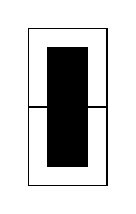
\begin{tikzpicture}[x=1.0cm, y=1.0cm]
        \draw (0,0) rectangle ++ (1,1);
        \draw (0,1) rectangle ++ (1,1);
        \draw[fill, black] (0.25 ,0.25) rectangle ++ (0.5,1.5);
    \end{tikzpicture}
\end{center}
当 $n = 2$ 时,我们有一个 $2 \times 2$ 棋盘。由于棋盘的方向很重要,因此我们有以下两种不同的密铺。因此,$T(2) = 2$。

\begin{center}
    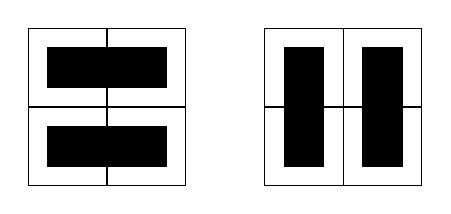
\begin{tikzpicture}[x=1.0cm, y=1.0cm]
        \foreach \y in {0,1} {
            \foreach \x in {0,1} {
                \draw (0+\x ,0+\y) rectangle ++ (1,1);
            }
        }

        \draw[fill, black] (0.25 ,0.25) rectangle ++ (1.5,0.5);
        \draw[fill, black] (0.25 ,1.25) rectangle ++ (1.5,0.5);

        \foreach \y in {0,1} {
            \foreach \x in {0,1} {
                \draw (3+\x ,0+\y) rectangle ++ (1,1);
            }
        }

        \draw[fill, black] (3+0.25 ,0.25) rectangle ++ (0.5,1.5);
        \draw[fill, black] (3+1.25 ,0.25) rectangle ++ (0.5,1.5);
    \end{tikzpicture}
\end{center}
当 $n = 3$ 时呢?同样地,我们可以手动枚举这些密铺,并确保没有遗漏任何一个。我们看到 $T(3) = 3$。

\begin{center}
    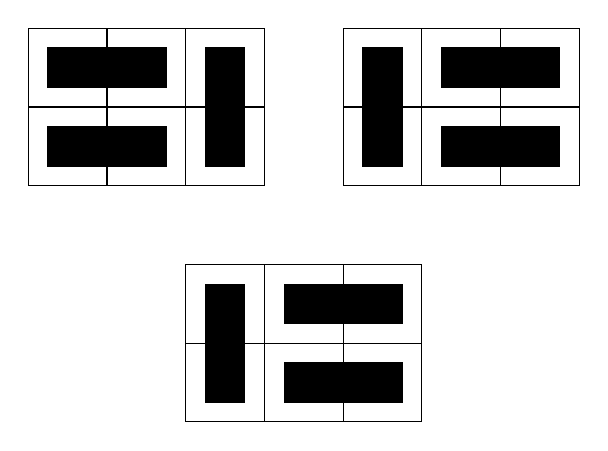
\begin{tikzpicture}[x=1.0cm, y=1.0cm]
        \foreach \y in {0,1} {
            \foreach \x in {0,1,2} {
                \draw (0+\x ,0+\y) rectangle ++ (1,1);
            }
        }

        \draw[fill, black] (0.25 ,0.25) rectangle ++ (1.5,0.5);
        \draw[fill, black] (0.25 ,1.25) rectangle ++ (1.5,0.5);
        \draw[fill, black] (2.25 ,0.25) rectangle ++ (0.5,1.5);

        \foreach \y in {0,1} {
            \foreach \x in {0,1,2} {
                \draw (4+\x ,0+\y) rectangle ++ (1,1);
            }
        }

        \draw[fill, black] (4+1.25 ,0.25) rectangle ++ (1.5,0.5);
        \draw[fill, black] (4+1.25 ,1.25) rectangle ++ (1.5,0.5);
        \draw[fill, black] (4+0.25 ,0.25) rectangle ++ (0.5,1.5);

        \foreach \y in {0,1} {
            \foreach \x in {0,1,2} {
                \draw (2+\x ,-3+\y) rectangle ++ (1,1);
            }
        }

        \draw[fill, black] (2+1.25 ,-3+0.25) rectangle ++ (1.5,0.5);
        \draw[fill, black] (2+1.25 ,-3+1.25) rectangle ++ (1.5,0.5);
        \draw[fill, black] (2+0.25 ,-3+0.25) rectangle ++ (0.5,1.5);
    \end{tikzpicture}
\end{center}
好的,再看一种情况,当 $n=4$ 时,我们看到 $T(4)=5$。

\begin{center}
    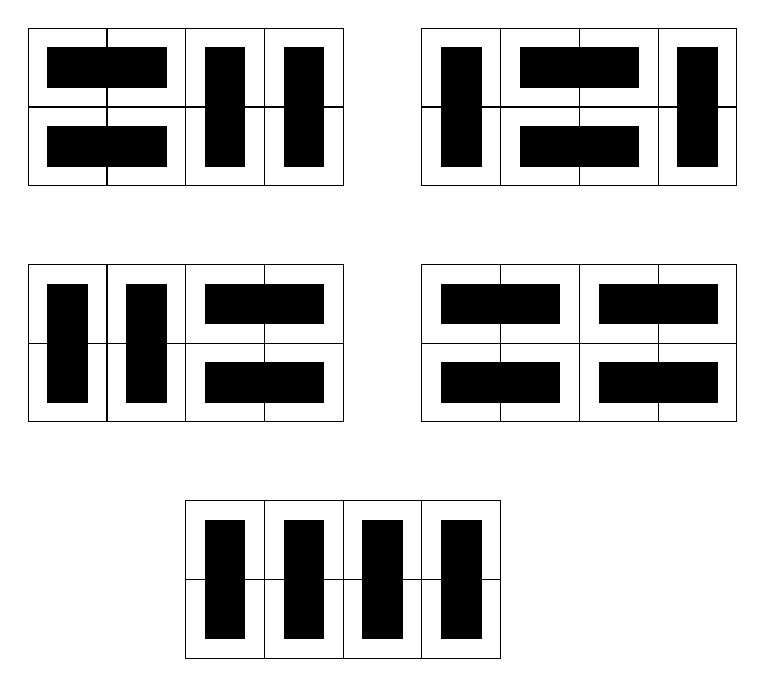
\begin{tikzpicture}[x=1.0cm, y=1.0cm]
        \foreach \y in {0,1} {
            \foreach \x in {0,...,3} {
                \draw (0+\x ,0+\y) rectangle ++ (1,1);
            }
        }

        \draw[fill, black] (0.25 ,0.25) rectangle ++ (1.5,0.5);
        \draw[fill, black] (0.25 ,1.25) rectangle ++ (1.5,0.5);
        \draw[fill, black] (2.25 ,0.25) rectangle ++ (0.5,1.5);
        \draw[fill, black] (3.25 ,0.25) rectangle ++ (0.5,1.5);

        \foreach \y in {0,1} {
            \foreach \x in {0,...,3} {
                \draw (5+\x ,0+\y) rectangle ++ (1,1);
            }
        }

        \draw[fill, black] (5+1.25 ,0.25) rectangle ++ (1.5,0.5);
        \draw[fill, black] (5+1.25 ,1.25) rectangle ++ (1.5,0.5);
        \draw[fill, black] (5+0.25 ,0.25) rectangle ++ (0.5,1.5);
        \draw[fill, black] (5+3.25 ,0.25) rectangle ++ (0.5,1.5);

        \foreach \y in {0,1} {
            \foreach \x in {0,...,3} {
                \draw (0+\x ,-3+\y) rectangle ++ (1,1);
            }
        }

        \draw[fill, black] (2.25 ,-3+0.25) rectangle ++ (1.5,0.5);
        \draw[fill, black] (2.25 ,-3+1.25) rectangle ++ (1.5,0.5);
        \draw[fill, black] (0.25 ,-3+0.25) rectangle ++ (0.5,1.5);
        \draw[fill, black] (1.25 ,-3+0.25) rectangle ++ (0.5,1.5);

        \foreach \y in {0,1} {
            \foreach \x in {0,...,3} {
                \draw (5+\x ,-3+\y) rectangle ++ (1,1);
            }
        }

        \draw[fill, black] (5+2.25 ,-3+0.25) rectangle ++ (1.5,0.5);
        \draw[fill, black] (5+2.25 ,-3+1.25) rectangle ++ (1.5,0.5);
        \draw[fill, black] (5+0.25 ,-3+0.25) rectangle ++ (1.5,0.5);
        \draw[fill, black] (5+0.25 ,-3+1.25) rectangle ++ (1.5,0.5);

        \foreach \y in {0,1} {
            \foreach \x in {0,...,3} {
                \draw (2+\x ,-6+\y) rectangle ++ (1,1);
            }
        }

        \draw[fill, black] (2+0.25 ,-6+0.25) rectangle ++ (0.5,1.5);
        \draw[fill, black] (2+1.25 ,-6+0.25) rectangle ++ (0.5,1.5);
        \draw[fill, black] (2+2.25 ,-6+0.25) rectangle ++ (0.5,1.5);
        \draw[fill, black] (2+3.25 ,-6+0.25) rectangle ++ (0.5,1.5);
    \end{tikzpicture}
\end{center}

我们现在可以开始寻找模式了吗?找到更大棋盘的密铺会很繁琐!让我们考虑一下如何利用 $T(1) = 1$ 的事实来推断出有关 $T(2)$ 的信息……等一下……做不到,对吧?这两个案例有本质的区别。具体来说,由于多米诺骨牌的大小为 $2 \times 1$,因此我们仅向棋盘中添加一行这一事实对我们没有帮助。

好吧,那么我们考虑 $n = 3$。我们可以利用 $T(2) = 2$ 这个事实吗?在这种情况下,答案是肯定的!知道 $2 \times 2$ 棋盘有两个密铺,无需太多思考,我们可以立即构建 $2 \times 3$ 棋盘的两个平铺。具体来说,我们可以将\emph{垂直多米诺骨牌添加}到之前的每一个密铺中。但我们知道 $T(3) = 3$。第三个密铺从何而来?再次查看该密铺,以及它与其他两个密铺的比较。在第三个密铺中,右侧的多米诺骨牌是水平的,而不是其他两种密铺中的垂直多米诺骨牌。如果我们移除这两个平行的水平多米诺骨牌,我们就会得到 $n = 1$ 时的情况。换句话说,我们可以通过在右侧\emph{添加一个由两个水平多米诺骨牌组成的正方形}来构建 $2 \times 3$ 棋盘的密铺。总的来说,我们已经用较小尺寸的棋盘(即 $2 \times 2$ 和 $2 \times 1$)描述了 $2 \times 3$ 棋盘的所有密铺:

\begin{center}
    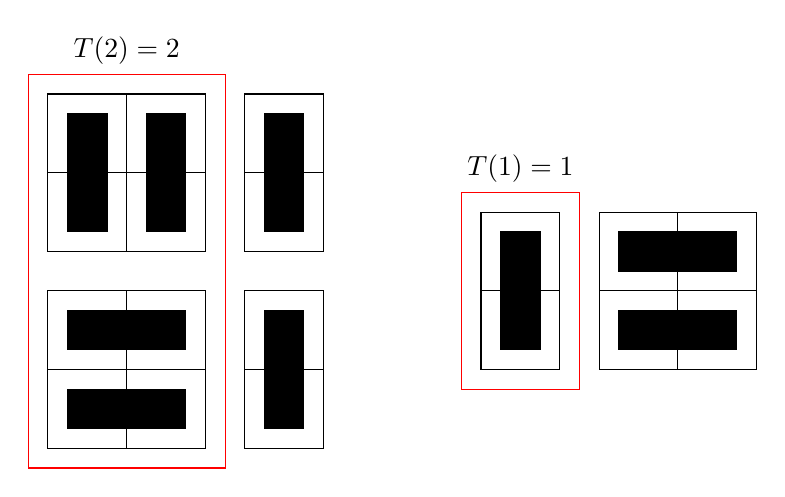
\begin{tikzpicture}[x=1.0cm, y=1.0cm]
        \foreach \g in {0, 2.5} {
            \foreach \y in {0,1} {
                \foreach \x in {0,1} {
                    \draw (0+\x ,0+\y+\g) rectangle ++ (1,1);
                }
            }
            \draw (2.5,0+\g) rectangle ++ (1,1);
            \draw (2.5,1+\g) rectangle ++ (1,1);
            \draw[fill, black] (2.75 ,0.25+\g) rectangle ++ (0.5,1.5);
        }

        \draw[fill, black] (0.25 ,0.25) rectangle ++ (1.5,0.5);
        \draw[fill, black] (0.25 ,1.25) rectangle ++ (1.5,0.5);

        \draw[fill, black] (0.25 ,2.5+0.25) rectangle ++ (0.5,1.5);
        \draw[fill, black] (1.25 ,2.5+0.25) rectangle ++ (0.5,1.5);

        \draw[red] (-0.25, -0.25) rectangle ++(2.5, 5);
        \path (-0.25,4.75) --  (2.25,4.75) node[midway,above,black] {$T(2)=2$};

        \draw (5.5,1) rectangle ++ (1,1);
        \draw (5.5,2) rectangle ++ (1,1);
        \draw[fill, black] (5.75 ,1.25) rectangle ++ (0.5,1.5);
        \draw[red] (5.25, 0.75) rectangle ++(1.5, 2.5);
        \path (5.25,3.25) --  (6.75,3.25) node[midway,above,black] {$T(1)=1$};

        \foreach \y in {0,1} {
            \foreach \x in {0,1} {
                \draw (7+\x ,1+\y) rectangle ++ (1,1);
            }
        }
        \draw[fill, black] (7.25 ,1.25) rectangle ++ (1.5,0.5);
        \draw[fill, black] (7.25 ,2.25) rectangle ++ (1.5,0.5);

    \end{tikzpicture}
\end{center}
\[T(3) = 3 = 2 + 1 = T(2) + T(1)\]

现在你可能会看出模式来!我们再看一下当 $n = 4$ 时会发生什么,我们将垂直多米诺骨牌添加到构成 $T(3)$ 的每一个密铺中,或者将两个水平多米诺骨牌添加到构成 $T(2)$ 的每一个密铺中,以此得到 $T(4)$ 的\emph{所有}密铺:

\begin{center}
    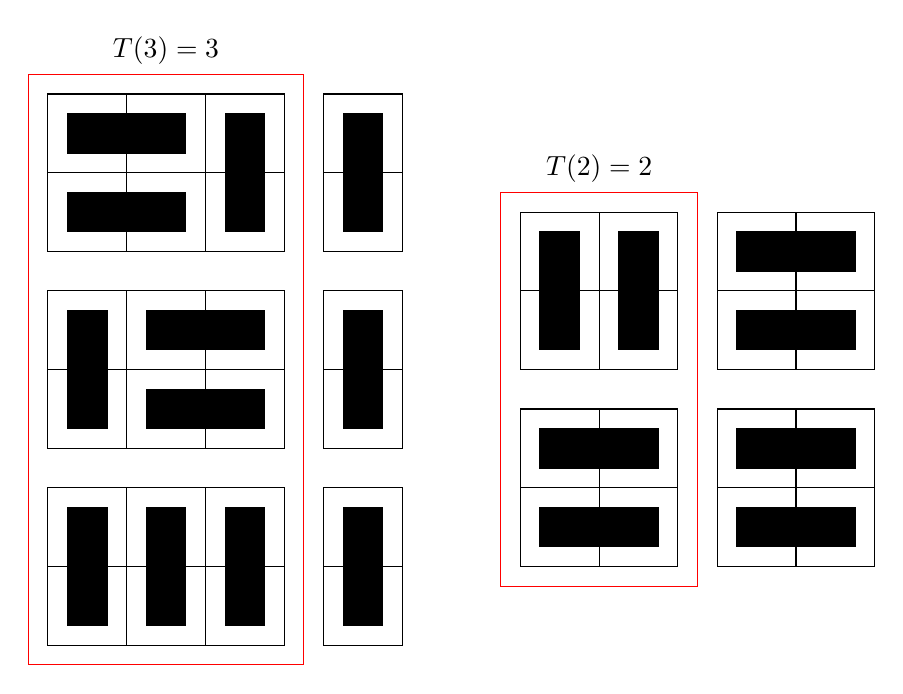
\begin{tikzpicture}[x=1.0cm, y=1.0cm]
        \foreach \g in {0, 2.5, 5} {
            \foreach \y in {0,1} {
                \foreach \x in {0,1,2} {
                    \draw (0+\x ,0+\y+\g) rectangle ++ (1,1);
                }
            }

            \draw (3.5,\g+0) rectangle ++ (1,1);
            \draw (3.5,\g+1) rectangle ++ (1,1);
            \draw[fill, black] (3.75 ,\g+0.25) rectangle ++ (0.5,1.5);
        }
        \draw[fill, black] (0.25 ,0.25) rectangle ++ (0.5,1.5);
        \draw[fill, black] (1.25 ,0.25) rectangle ++ (0.5,1.5);
        \draw[fill, black] (2.25 ,0.25) rectangle ++ (0.5,1.5);

        \draw[fill, black] (0.25 ,2.75) rectangle ++ (0.5,1.5);
        \draw[fill, black] (1.25 ,2.75) rectangle ++ (1.5,0.5);
        \draw[fill, black] (1.25 ,3.75) rectangle ++ (1.5,0.5);

        \draw[fill, black] (2.25 ,5.25) rectangle ++ (0.5,1.5);
        \draw[fill, black] (0.25 ,5.25) rectangle ++ (1.5,0.5);
        \draw[fill, black] (0.25 ,6.25) rectangle ++ (1.5,0.5);

        \draw[red] (-0.25, -0.25) rectangle ++(3.5, 7.5);
        \path (-0.25,7.25) --  (3.25,7.25) node[midway,above,black] {$T(3)=3$};


        \foreach \g in {0, 2.5} {
            \foreach \y in {0,1} {
                \foreach \x in {0,1} {
                    \draw (6+\x ,1+\y+\g) rectangle ++ (1,1);
                }
            }
            \foreach \y in {0,1} {
                \foreach \x in {0,1} {
                    \draw (8.5+\x ,1+\y+\g) rectangle ++ (1,1);
                }
                \draw[fill, black] (8.75 ,1.25+\g+\y) rectangle ++ (1.5,0.5);
            }
           
        }

        \draw[fill, black] (6.25 ,1.25) rectangle ++ (1.5,0.5);
        \draw[fill, black] (6.25 ,2.25) rectangle ++ (1.5,0.5);

        \draw[fill, black] (6.25 ,3.5+0.25) rectangle ++ (0.5,1.5);
        \draw[fill, black] (7.25 ,3.5+0.25) rectangle ++ (0.5,1.5);

        \draw[red] (5.75, 0.75) rectangle ++(2.5, 5);
        \path (5.75,5.75) --  (8.25,5.75) node[midway,above,black] {$T(2)=2$};
        
    \end{tikzpicture}
\end{center}
\[T(4) = 5 = 3 + 2 = T(3) + T(2)\]

另请注意,用这种方式不会产生重复的 $2 \times 4$ 密铺。(仔细想想为什么会这样。我们用一种什么方法表征两种密铺可以保证它们不重复?)有了这些信息,我们可以立即得出结论 $T(4) = T(3) + T(2)$。

此外,我们可以概括这样一个论点;$n = 4$ 没有什么特别的,对吧?对于任意特定的 $n$,我们可以只考虑所有可能的密铺,然后看看棋盘\emph{最右侧}发生的情况:要么有一个垂直多米诺骨牌(这意味着密铺来自 $2 \times (n - 1)$ 棋盘),要么有两个水平多米诺骨牌(这意味着密铺来自 $2 \times (n-2)$ 棋盘)。有了这个论点的支撑,对于所有有意义的 $n$ 值,我们可以得出如下结论:
\[T(n) = T(n - 1) + T(n - 2)\]
哪些 $n$ 值有意义?请记住,我们必须单独分析 $T(1)$ 和 $T(2)$;因此这个论点不适用于 $n=1$ 和 $n=2$,我们必须添加限制条件 $n \ge 3$ 才能使上面公式成立。

有了这些信息,只要有足够的时间,我们就可以轻松计算出任意 $n$ 值下的 $T(n)$。我们甚至可以相当容易地编写出计算机程序。然而,正是这种\emph{归纳}论证——我们注意到的模式以及我们对其发生原因的彻底描述——让我们首先得出了结论。这种情况下,每一项的值 $T(n)$ 取决于前\emph{两}项 $T(n-1)$ 和 $T(n-2)$ 的值。这在本章之前的例子中\emph{没有}出现过,它暗示了这里发生了更深层次的事情。你是否发现我们之前对归纳的定义以及多米诺骨牌的类比在这里不再适用?你会如何修正我们的类比来解释这种情况?思考一下这些问题,然后继续阅读。我们将在下一个示例之后更深入地讨论它们。

顺便一提,你是否注意到此示例的解有一些有趣的地方?你还知道其他类似的数列吗?想一想……


% !TeX root = ../../../book.tex
\subsection{制胜策略}

这个例子将是我们第一个\emph{无需}证明数值公式的归纳问题!这似乎有些奇怪,但正如即将看到的,事实确实如此。实际上在数学中,这种情况比你想象的更为常见:一个问题或数学对象可能蕴含潜在的归纳结构,却并不依赖代数或算术的具体内容。

具体来说,我们将讨论一个\emph{游戏}。它是通常意义上的游戏——有玩家必须遵守的规则以及明确的胜负判定——同时也是数学意义上的游戏:我们可以用数学符号精确描述规则和情境,并抽象地探讨\emph{策略},甚至能\emph{解}出这个游戏。这与棒球比赛截然不同。

现在介绍游戏规则,我们暂且称之为``取石子''。有两名玩家 $P_1$ 和 $P_2$,$P_1$ 先行。桌上有两堆石子,每堆恰好有 $n$ 个($n$ 为自然数)。为区分不同版本,当每堆石子数为 $n$ 时,我们称玩家在进行``$T_n$ 游戏''。每回合玩家可从\emph{任意}一堆取走\emph{任意}数量的石子(不可同时取两堆)。取走\emph{最后}一颗石子者\emph{获胜}。

试着跟朋友玩一下这个游戏。用硬币或糖果代替石子,并试着互换 $P_1$/$P_2$ 角色。尝试制定获胜\emph{策略}——最大化胜率的玩法,推测不同 $n$ 值下的胜负关系。谁``应该''获胜?能否给出\emph{证明}?请务必先亲自体验游戏并尝试给出证明,再继续阅读我们的分析。你可能会惊讶于自己的发现!

与其他示例一样,我们先观察 $n$ 为较小数值的情形再进行推广。当 $n = 1$ 时,游戏很简单:$P_1$ 只能取走其中一堆的唯一石子,随后 $P_2$ 取走另一堆的石子获胜。(注意:无论 $P_1$ 选择哪堆,$P_2$ 总能取走剩余的石子。我们可以说``不失一般性'',假设 $P_1$ 选左堆,因为两堆等价。后文讨论数理逻辑时,我们将深入探讨``不失一般性''这一概念。)

\begin{center}
    \begin{tikzpicture}[line width=0.5mm]
        \foreach \n in {0, 1}{
            \node at (\n, 0)[circle,fill,inner sep=8pt, anchor=west]{};
            \draw (\n, -1) -- +(0.8, 0);
        }
        \draw[-latex] (2.5, -0.4) -- +(2, 0) node[midway,above]{$P_1$ 回合};
        \draw (5, -1) -- +(0.8, 0);
        \node at (6, 0)[circle,fill,inner sep=8pt, anchor=west]{};
        \draw (6, -1) -- +(0.8, 0);
        \draw[-latex] (7.5, -0.4) -- +(2, 0) node[midway,above]{$P_2$ 回合};
        \draw (10, -1) -- +(0.8, 0);
        \draw (11, -1) -- +(0.8, 0);
        \path (10, -0.4) -- +(2, 0) node[midway,above]{$P_2$ 胜!};
    \end{tikzpicture}
\end{center}

当 $n = 2$ 时,可能出现几种情况。考虑玩家 $P_1$ 可能的行动。虽然 $P_1$ 可选择左堆或右堆,但由于最终结果相同且两堆可交换,不妨设(不失一般性)$P_1$ 从左堆取走若干石子。具体而言,可能取一颗或两颗石子。下面对每种情况分别讨论。

\begin{center}
    \begin{tikzpicture}[line width=0.5mm]
        \foreach \x in {0, 1}{
            \node at (\x, 0)[circle,fill,inner sep=8pt, anchor=west]{};
            \node at (\x, 1)[circle,fill,inner sep=8pt, anchor=west]{};
            \draw (\x, -1) -- +(0.8, 0);
        }
        \draw[-latex] (2.5, -0.4) -- +(2, -0.6);
        \draw[-latex] (2.5, 0.6) -- +(2, 0.6);
        \node[anchor=west] at(2.5,0) {$P_1$ 回合};
        \foreach \delta in {1, -2}{
            \foreach \n in {0, 1}{
                \draw (5+\n, \delta) -- +(0.8, 0);
                \node at (6, \delta+1+\n)[circle,fill,inner sep=8pt, anchor=west]{};
            }
        }
        \node at (5, -1)[circle,fill,inner sep=8pt, anchor=west]{};
        \draw[-latex] (7.5, 2) -- +(2, 0) node[midway,above]{$P_2$ 回合};
        \draw[-latex] (7.5, -1) -- +(2, 0) node[midway,above]{$P_2$ 回合};
        \draw (10, 1) -- +(0.8, 0);
        \draw (11, 1) -- +(0.8, 0);
        \path (10, 1.6) -- +(2, 0) node[midway,above]{$P_2$ 胜!};
        \path (10, -1.4) -- +(2, 0) node[midway,above]{???};
    \end{tikzpicture}
\end{center}

若 $P_1$ 取走两颗石子,$P_2$ 应该如何应对?此时 $P_2$ 可以取走另一堆的全部石子从而获胜,因此 $P_1$ 不应采取此行动。但为全面分析游戏,仍需考虑所有可能情况。故在此情形下(对应示意图上半部分),$P_2$ 获胜。此情况较为简单。

若 $P_1$ 仅从左堆取走一颗石子(对应示意图下半部分),$P_2$ 应该如何应对?此时存在多种选择:

\begin{itemize}
    \item 若 $P_2$ 从左堆取走最后一颗石子,则 $P_1$ 可以取走右堆全部石子获胜。
    \item 若 $P_2$ 从右堆取走全部两颗石子,则 $P_1$ 可以取走左堆最后一颗石子获胜。
    \item 若 $P_2$ 仅从右堆取走一颗石子……
\end{itemize}

\begin{center}
    \begin{tikzpicture}[line width=0.5mm]
        \foreach \g in {0, 5, 10} {
            \foreach \x in {0, 1} {
                \node at (\x+\g, 0)[circle,fill,inner sep=8pt, anchor=west]{};
                \draw (\x+\g, -1) -- +(0.8, 0);
            }
        }
        \node at (0, 1)[circle,fill,inner sep=8pt, anchor=west]{};
        \node at (1, 1)[circle,fill,inner sep=8pt, anchor=west]{};
        \draw[-latex] (2.5, -0.4) -- +(2, 0) node[midway,above]{$P_1$ 回合};

        \node at (6, 1)[circle,fill,inner sep=8pt, anchor=west]{};
        \draw[-latex] (7.5, -0.4) -- +(2, 0) node[midway,above]{$P_2$ 回合};
    \end{tikzpicture}
\end{center}

此时局面与 $T_1$ 完全相同,而该情形已分析过:由于此时轮到 $P_1$ 行动,无论其如何操作,$P_2$ 都将获胜。对 $P_2$ 而言,此乃最优应对——\emph{无论} $P_1$ \emph{采取何种行动},$P_2$ 均可获胜!

综上可见:无论 $P_1$ 初始采取何种行动(从任意堆取一或两颗石子),$P_2$ 总能作出\emph{特定回应以保证获胜},且此后无论 $P_1$ 如何应对均无法改变结果。$P_2$ 已占据不败之地。现在让我们进一步探究其他 $n$ 值的情形。

当 $n = 3$ 时,我们再次不失一般性地假设玩家 $P_1$ 首先从左侧石子堆取石子。他可以取走一颗、两颗或三颗石子:
\begin{itemize}
    \item 若 $P_1$ 取走全部三颗石子,则 $P_2$ 将直接取走另一堆石子并获胜。
    \item 若 $P_1$ 取走两颗石子……此时 $P_2$ 应该如何应对?
\end{itemize}
$P_2$ 若取空右侧堆是愚蠢的($P_1$ 随后可取空左侧堆获胜),同样取空左侧堆也不明智($P_1$ 可以立即取空右侧堆获胜),因此需采取折中策略。若 $P_2$ 仅从右侧堆取走一颗石子,$P_1$ 可采取相同策略回应,导致两堆均剩一颗石子且轮次互换——此时 $P_2$ 成为先手方。根据此前分析,$P_2$ 在此局面下必败,因此这是一个糟糕的策略!

\begin{center}
    \begin{tikzpicture}[line width=0.5mm]
        \foreach \g in {0, 5, 10, 15}{
            \foreach \x in {0, 1}{
                \node at (\x+\g, 0)[circle,fill,inner sep=8pt, anchor=west]{};
                \draw (\x+\g, -1) -- +(0.8, 0);
            }
        }
        \foreach \x in {0, 1, 6}{
            \foreach \y in {0, 1}{
                \node at (\x, \y)[circle,fill,inner sep=8pt, anchor=west]{};
                \node at (\x, \y+1)[circle,fill,inner sep=8pt, anchor=west]{};
            }
        }

        \node at (11, 1)[circle,fill,inner sep=8pt, anchor=west]{};

        \draw[-latex] (2.5, -0.4) -- +(2, 0) node[midway,above]{$P_1$ 回合};
        \draw[-latex] (7.5, -0.4) -- +(2, 0) node[midway,above]{$P_2$ 回合};
        \draw[-latex] (12.5, -0.4) -- +(2, 0) node[midway,above]{$P_1$ 回合};
        \path (15, 0.6) -- +(2, 0) node[midway,above]{$P_1$ 胜!};
    \end{tikzpicture}
\end{center}

让我们重新推演:若 $P_2$ 从右侧堆取走两颗石子……局面立现转机!此时每堆仅余一颗石子,$P_1$ 作为先手必败,$P_2$ 锁定胜局!

\begin{center}
    \begin{tikzpicture}[line width=0.5mm]
        \foreach \g in {0, 5, 10}{
            \foreach \x in {0, 1}{
                \node at (\x+\g, 0)[circle,fill,inner sep=8pt, anchor=west]{};
                \draw (\x+\g, -1) -- +(0.8, 0);
            }
        }
        \foreach \x in {0, 1, 6}{
            \foreach \y in {0, 1}{
                \node at (\x, \y)[circle,fill,inner sep=8pt, anchor=west]{};
            }
        }
        \draw[-latex] (2.5, -0.4) -- +(2, 0) node[midway,above]{$P_1$ 回合};
        \draw[-latex] (7.5, -0.4) -- +(2, 0) node[midway,above]{$P_2$ 回合};
        \path (10, 0.6) -- +(2, 0) node[midway,above]{$P_2$ 胜!};
    \end{tikzpicture}
\end{center}

考虑 $n = 4$ 的情形,类似分析依然适用。玩家 $P_1$ 可以从左侧堆取走一至四颗石子。但无论其如何操作,$P_2$ 皆可在另一堆上\emph{模仿}相同动作,将游戏简化为更小规模的已知局面,从而确保胜利!$P_2$ 似乎始终占据主动:他能通过镜像策略回应 $P_1$ 的任何操作。无论 $P_1$ 采取何种行动,$P_2$ 的针对性回应终将导向胜利。因此我们称``$P_2$ 拥有必胜策略''——其具备明确的方法评估局势并选择特定行动以\emph{确保获胜}。

我们要如何证明这一点?如何运用本章的归纳法?目前或许难以窥见全貌。我们究竟需要证明什么?此处的多米诺骨牌或阶梯类比如何具象化?思考这个案例时需领悟:归纳法不仅关乎代数表达式,更体现某种``递推''结构,即大规模情形依赖于小规模情形;我们需先证明初始事实,再论证如何将任意更大规模情形化归为已证事实。这才是多米诺类比的本质。该类比虽能有效阐释部分归纳问题(非全部)且具有直观感染力,但并非普适于\emph{所有}场景。

回顾本章给出的四个案例,辨析其异同。尝试用更精准的数学语言(或自创术语)描述数学归纳法(需超越直观类比)。令人惊叹的是,即使尚未掌握``标准''表述,但你仍能通过此过程深化理解并获得精妙描述!后续我们将严格陈述并证明数学归纳法及其变体。在此之前,需先探索其他数学领域以构建必要的语言、符号与知识基础。不过启程之前,不妨先了解一下数学归纳法的若干经典应用。


% !TeX root = ../../../book.tex
\subsection{习题}

\subsubsection*{温故知新}

以口头或书面的形式简要回答以下问题。这些问题全都基于你刚刚阅读的内容,所以如果忘记了具体的定义、概念或示例,可以回去重读相关部分。确保在继续学习之前能够自信地回答这些问题,这将有助于你的理解和记忆!

\begin{enumerate}[label=(\arabic*)]
    \item 这两个例子如何\emph{归纳}?它们在哪些方面与前面的例子(立方体和直线)相似?哪些方面有所不同?
    \item 对于多米诺骨牌密铺问题,我们需要知道多少个先前值才能计算 $T(n)$?
    \item $T(n) = T(n - 1) + T(n - 2)$ 和 $T(n + 2) = T(n + 1) + T(n)$ 有什么区别?
    \item 取石子游戏的必胜策略是什么?尝试与一个不了解该游戏的朋友一起玩一下,并使用玩家 $P_2$ 的必胜策略。每次你都获胜时他们有多沮丧?他们也开始发现这个策略了吗?
\end{enumerate}

\subsubsection*{小试牛刀}

尝试回答以下问题。这些题目要求你实际动笔写下答案,或(对朋友/同学)口头陈述答案。目的是帮助你练习使用新的概念、定义和符号。题目都比较简单,确保能够解决这些问题将对你大有帮助!

\begin{enumerate}[label=(\arabic*)]
    \item $T(5)$ 会是怎样?你能画出所有密铺方案吗?
    \item 探讨用两堆各 $4$ 颗石子进行取石子游戏的可能性。你能确保玩家 $P_2$ 总是有必胜策略吗?
    \item \textbf{挑战题:}如果用\emph{三堆}相同大小的石子来玩``取石子''游戏,会发生什么?你能为任意一方找到获胜策略吗?尝试和朋友一起玩一下,看看会发生什么!
    \item 查看\emph{斐波那契数列}。它与我们在多米诺骨牌密铺示例中发现的数列 $T(n)$ 有什么关系?
\end{enumerate}

\newpage
% !TeX root = ../../../book.tex
\section{应用}

% !TeX root = ../../../book.tex
\subsection{递归程序}\label{sec:section2.5.1}

数学归纳法背后的概念也大量应用于计算机科学中。回想一下我们当初是如何推导出 $\sum_{k=1}^{n}k^2$ 的公式的。一旦我们找到了用更小的立方和剩余项来表示立方数的方法,我们就会一遍又一遍地重复这个替代过程,直到我们到达``最简单''的情况,即我们在开始计算问题:$2^3=1+3+3+1$ 时第一次观察到的情况。递归编程利用了这一技术:为了解决``大''问题,确定问题如何依赖于``小''案例,并化简问题,直到达到一个简单的已知案例。

此类技术的一个经典示例是编写代码来计算\emph{阶乘} $n!$,它被定义为前 $n$ 个自然数的乘积:
\[n! = 1 \cdot 2 \cdot 3 \dots (n - 1) \cdot n\]
这是一个简单的定义,我们作为人类可以直观地理解,但告诉计算机如何执行该产品的方式并不完全相同。(尝试一下!怎么用计算机代码表达``继续执行,直到达到 $n$''?)事实上,对函数进行编程的一种更有效的方法,以及对数学归纳定义进行建模的方法,是让一个程序\emph{递归地调用自身},直到达到``最简''情况。在阶乘种,这种情况就是 $1! = 1$。对于 $n$ 的任意其他值,我们可以简单地不断应用以下知识:
\[n! = (n - 1)! \cdot n\]
来计算 $n!$。下面的\emph{伪代码}描述了这一思想:

\begin{verbatim}
    factorial(n):
        if n = 1
            return 1
        else
            return n * factorial(n-1)
    end
\end{verbatim}

我们知道 $1! = 1$,因此如果要求程序计算该值,则会立即返回正确的结果。对于任意大于 $1$ 的 $n$ 值,程序都会引用\emph{自身},并说:``为我计算 $(n-1)!$,然后我在后面乘上 $n$ 就得到答案了。''为了计算 $(n-1)!$,程序会再次询问输入是否为 $1$;如果不为 $1$,则会继续调用自身并说:``为我计算 $(n-2)!$,然后我在后面乘上 $(n-1)$ 。'' 这个过程一直持续到程序返回 $1! = 1$。从那之后,程序就知道如何求出 $2! = 1 \times 2$,然后是 $3! = 2! \times 3$,依此类推,直到 $n! = (n - 1)! \times n$。

递归编程的另一个经典例子是\emph{斐波那契数}。可能你之前在数学课上见过这个数列。(事实上,我们在上一节多米诺骨牌密铺中提到过该数列!)你可能还听说过斐波那契数列以一些有趣和奇怪的方式出现在自然界中。(该数列最早是由比萨的意大利数学家莱昂纳多·斐波那契(Leonardo Fibonacci)在研究兔子种群增长时``发现''的。)斐波那契数列的前两项均为 $1$,数列中的任意数字都被定义为前两个数字之和。也就是说,如果我们用 $F(n)$ 表示第 $n$ 个斐波那契数,那么
\[F(1) = 1 \text{ 且 }F(2) = 1, \text{ 对于任意 } n \ge 3, F(n) = F(n - 1) + F(n - 2)\]
那么,$F(5)$ 等于多少?$F(100)$ 呢?$F(10000)$ 呢?这可以通过递归程序很容易地处理。思路是一样的:如果程序遇到``简单情况''之一,即 $F(1)$ 或 $F(2)$,则立即返回正确值 $1$。否则,将调用自身来计算前两个数字,然后将它们相加。阅读下面的伪代码并思考它是如何工作的。如果我们使用这个程序来计算 $F(10)$ 会发生什么?怎样才能得出答案呢?

\begin{verbatim}
    Fibonacci(n):
        if n = 1 or n = 2
            return 1
        else
            return Fibonacci(n-1) + Fibonacci(n-2)
    end
\end{verbatim}

上面程序与 \verb|factorial| 程序的思路相同(让程序调用自身来计算函数``较小''情况的值,直到达到已知值),但这里有一些更深层次的内容。但这里有一些更深层次的内容。如果我们将 $n = 10$ 输入到程序中,它会识别出还不知道应该输出什么值,于是会调用自身来计算 \verb|Fibonacci(9)| 和 \verb|Fibonacci(8)|。对程序的每次调用,都会再次识别出该值未知。因此,会再次调用自身来计算 \verb|Fibonacci(8)| 和 \verb|Fibonacci(7)|,以及 \verb|Fibonacci(7)| 和 \verb|Fibonacci(6)|。没错,程序使用相同的输入值多次调用自身。为了计算 $F(9)$,我们需要知道 $F(8)$ 和 $F(7)$,但同时,为了计算 $F(8)$,我们还需要知道 $F(7) $ 和 $F(6)$。这样,我们最终多次调用程序 \verb|Fibonacci|。

尝试比较 \verb|Fibonacci| 程序和 \verb|factorial| 程序,特别是关于我们在本章中研究的归纳过程。他们使用类似的思路吗? 它们与我们介绍数学归纳法时用到的``多米诺骨牌''类比有何关系?将多米诺骨牌 $n$ 上的``事实''视为对 $n!$ 的正确计算或 $F(n)$。这个类比在每种情况下如何发挥作用?所有多米诺骨牌都会倒下吗?在你继续阅读时,请记住这些问题。所有这些想法背后都有一些非常强大的数学基础。

\clearpage


% !TeX root = ../../../book.tex
\subsection{汉诺塔}

我们稍作休息来玩个游戏吧。虽然严格来说不算完全放松——因为它本质上是关于\emph{归纳}的练习,所以与主题密切相关——但至少是个游戏!\emph{汉诺塔}作为经典智力游戏广受欢迎,部分得益于其简洁的规则和道具。然而它的解法可绝不简单!

假设有三根垂直立柱,以及三个大小不同的圆盘(\textcolor{blue}{蓝色}、\textcolor{olivegreen}{绿色}、\textcolor{red}{红色})叠放其中,初始状态如下:
\begin{center}
    \begin{tikzpicture}[line width=4mm,line cap=round,xscale=3,brown!30]
        \def\sequence{3/1,2/1,1/1}
        % init colors
        \foreach[count=\j] \c in {red,olivegreen,blue}
            \gset col[\j]={\c};
        \edef\numdisks{\j}
        % init positions and draw support
        \foreach \j in {1,2,3}{
            \gset pos[\j]=0
            \draw (\j,-.4) -- +(0,3);
        }
        \draw (.5,-.4) -- +(3,0);

        % draw
        \foreach[count=\k] \i/\j in \sequence{
            \edef\delta{\i*0.4/3}
            \draw[draw={\get col[\i]}](\j-\delta,\get pos[\j]) -- (\j+\delta,\get pos[\j]);
            \ginc pos[\j]+={.4}
        }
    \end{tikzpicture}
\end{center}
目标是将所有圆盘移至另一立柱(左中右皆可),但需遵守两条规则:
\begin{enumerate}
    \item 每次只能移动一个圆盘,且必须从某立柱顶端移至另一立柱顶端;
    \item 任何圆盘不可置于比它小的圆盘之上。
\end{enumerate}
规则虽简,破解却难!建议用硬币或扑克牌模拟(亦可购买专用套件)。你能破解这个问题吗?用了多少步?这是最优解吗?原因何在?

既然这是归纳游戏,我们深入探究:解决此谜题需多少步?(一步指单个圆盘的移动)更关键的是,如何确定\emph{最小步数}?以三个圆盘为例,若反复移动最小圆盘 $100$ 次后再求解,显然非最优。那么如何证明某种解法的步数已达最小值?

为了解决这个问题,我们将尝试\emph{递归分解}解法。此过程能回答更一般的问题:$n$ 个圆盘在三柱汉诺塔中的最小移动步数是多少?以 $3$ 个圆盘引入是为了便于理解,但通过深入分析可解决一般情况。为确保理解一致,先演示 $3$ 个圆盘的解法:

\begin{center}
    \begin{tikzpicture}[line width=2.6mm,line cap=round,xscale=1.5,yscale=0.5,brown!30]
        \def\sequencelist{{3/1,2/1,1/1}, {3/1,2/1,1/3}, {3/1,2/2,1/3}, {3/1,2/2,1/2}, {3/3,2/2,1/2}, {3/3,2/2,1/1}, {3/3,2/3,1/1}, {3/3,2/3,1/3}}
        % init colors
        \foreach[count=\j] \c in {red,olivegreen,blue}
            \gset col[\j]={\c};
        \edef\numdisks{\j}
        \foreach[count=\n] \sequence in \sequencelist {
            % init positions and draw support
            \foreach \j in {1,2,3}{
                \gset pos[\j]=0
                \draw (\j,-0.4-5*\n) -- +(0, 3);
            }
            \draw (0.5,-0.52-5*\n) -- +(3,0);
            % draw
            \foreach[count=\k] \i/\j in \sequence{
                \edef\delta{\i*0.4/3}
                \draw[draw={\get col[\i]}](\j-\delta,\get pos[\j]-5*\n) -- (\j+\delta,\get pos[\j]-5*\n);
                \ginc pos[\j]+={0.52}
            }
        }
        \node[black,left] at (0,-5.52){开始};
        \foreach \m in {1, ..., 7} {
            \node[black,left] at (0,-5.52-5*\m){第 \m 步};
        }   
    \end{tikzpicture}
\end{center}

请注意,最大的圆盘在多数解法中几乎是``无关紧要''的。由于我们可以在其上放置任何其他圆盘,我们只需将其他圆盘移到不同立柱上以``露出''最大圆盘,将其移至唯一的空立柱,再将其他圆盘移回即可。本质上,我们重复执行相同过程(将两个较小圆盘从一个立柱移至另一个立柱)两次,中间移动一次最大圆盘。若最大圆盘不存在,我们所做的正是解决两次 $2$ 盘问题!(仔细思考这一点,确保理解上文。可设想最大的\textcolor{blue}{蓝色}圆盘不存在,操作一遍上图的步骤。)

这表明解决 $3$ 盘问题需两次迭代解决 $2$ 盘问题,并增加一次移动最大圆盘的操作。一般而言,这揭示了问题的\emph{递归}性质:为得到 $n$ 盘问题的最优解,只需遵循解决 $(n-1)$ 盘问题的最优过程,移动一次最大的第 $n$ 个圆盘,再解决一次 $(n-1)$ 盘问题。

了解解法后,让我们确定所需步数。由于该问题需用\emph{递归}算法,任何关于最优解的\emph{证明}都需使用\emph{归纳法}。因此需要确定`起点'',即问题的``最小''或``最简''形式。对汉诺塔而言,最简形式是 $1$ 盘问题——只需一步将圆盘移至另一个立柱即可。若用 $M(n)$ 表示解决 $n$ 盘问题的最少移动次数,则 $M(1)=1$。根据前述观察:
\[\underbrace{M(2)}_{2 \text{盘问题}}= \underbrace{M(1)}_{1 \text{盘问题}}+ \underbrace{1}_{\text{移动最大圆盘}}+ \underbrace{M(1)}_{1 \text{盘问题}}= 1 + 1 + 1 = 3\]
进而可得:
\[M(3) = M(2) + 1 + M(2) = 3 + 1 + 3 = 7\]
和
\[M(4) = M(3) + 1 + M(3) = 7 + 1 + 7 = 15\]
以此类推。你发现规律了吗?这些数均为 $2$ 的幂减 $1$,即 $M(n)=2^n-1$。需指出,观察到规律不等于证明规律——它仅在前 $4$ 种情况成立,而归纳法将证明其普遍性。发现 $M(n)=2^n-1$ 本身已是重要洞见。你可以尝试求解以下递推关系:
\[M(n) = 2M(n - 1) + 1 \quad \text{且} \quad M(1) = 1\]
看看能否推导出公式 $M(n) = 2^n -1$。此闭合式优于递推式,因为 $M(n)$ 仅依赖 $n$ 而非前项(例如 $M(n-1)$)。此类关系称为\emph{递推关系},通常求解困难!

我们已知 $M(n)=2^n-1$,但验证工作留给你来完成。虽可代入数值检验,但这并非\emph{证明}。请尝试用归纳法严格证明!我们已完成了主体工作,但还需要你严谨地将一切串联在一起。请记住,你需要明确每张多米诺骨牌上的``事实''是什么,确保多米诺骨牌 $1$ 会倒下,然后对多米诺骨牌 $n$ 倒下会引起多米诺骨牌 $(n+1)$ 倒下进行一般性论证。试着写出这个证明。这些细节对你来说是否合理?向朋友展示你的证明,看看他们是否理解。你还需要向他们做出解释或指导他们完成证明阅读吗?思考最佳的解释方法与步骤,确保书面版本清晰准确。

\clearpage


% !TeX root = ../../../book.tex
\subsection{习题}

\subsubsection*{温故知新}

以口头或书面的形式简要回答以下问题。这些问题全都基于你刚刚阅读的内容,如果忘记了具体定义、概念或示例,可以回顾相关内容。确保在继续学习之前能够自信地作答这些问题,这将有助于你的理解和记忆!

\begin{enumerate}[label=(\arabic*)]
    \item 递归程序如何进行归纳?
    \item 汉诺塔的归纳结构是什么?在解决 $3$ 盘问题时,我们是如何处理 $2$ 盘问题的?
\end{enumerate}

\subsubsection*{小试牛刀}

尝试解答以下问题。这些题目需动笔书写或口头阐述答案,旨在帮助你熟练运用新概念、定义及符号。题目难度适中,确保掌握它们将大有裨益!

\begin{enumerate}[label=(\arabic*)]
    \item 根据伪代码 \verb|factorial| 的步骤计算 $5!$。
    \item 根据伪代码 \verb|Fibonacci| 的步骤计算 $F(5)$。
    \item 解决 $4$ 盘汉诺塔问题。确保你能以\emph{最优}步数 $2^4 - 1 = 15$ 步完成。
\end{enumerate}

\newpage
% !TeX root = ../../../book.tex
\section{总结}

我们已经了解了一些\textbf{归纳证明}的实例。通过解决具有相似证明模式的问题并研究不同案例,我们认识到这些证明可能涉及多样化的情境。具体而言,我们发现归纳证明\emph{并非}仅适用于求和公式或等式:它可应用于\emph{任何}依赖``先前事实''的情形。这促使我们从数学角度思考归纳法的运作机制。虽然``多米诺骨牌类比''目前是我们理解归纳法的直观方式,但接下来的核心目标是严格\emph{陈述}并\emph{证明}归纳原理。当前阶段,我们需要通过大量练习来掌握此类证明,这正是本章习题的设计目的。待后续形式化归纳法后,我们将能更熟练地运用它,并深化对这一概念的理解!

\newpage
% !TeX root = ../../../book.tex
\section{本章习题}

以下问题,有助于你熟悉归纳证明。我们暂不要求完全严格的证明,只需清晰地描述过程并写出步骤即可。待掌握数学归纳原理 (PMI) 及相应证明策略后,可重新严格证明这些问题。

\begin{exercise} \label{exc:exercises2.7.1}
    证明以下求和公式对所有自然数 $n$(包括 $n=0$)成立:
    \[\sum_{i=0}^{n}2^i=2^{n+1}-1\]
    后续问题:利用此结果说明在 $2^n$ 支球队的单场淘汰赛中,需进行多少场比赛才能决出冠军?(例如 NCAA 疯狂三月锦标赛就采用此赛制,其中 $n=6$。)
\end{exercise}

\begin{exercise}
    证明对于每个大于等于 $2$ 的自然数 $n$,均有 $3^n \ge 2^{n+1}$。
\end{exercise}

\begin{exercise}
    判断下列不等式对哪些自然数 $n$ 成立?先陈述结论,再予以证明。
    \begin{enumerate}
        \item $2^n \ge (n + 1)^2$
        \item $2^n \ge n!$
        \item $3^{n+1} > n^4$
        \item $n^3 + (n + 1)^3 > (n + 2)^3$
    \end{enumerate}
\end{exercise}

\begin{exercise}
    \textbf{末日游戏}:两名玩家轮流在日历上命名日期。每回合玩家可增加月份或日期(但不可同时增加)。从 1 月 1 日开始,说出 12 月 31 日者获胜。确定先手玩家的必胜策略。例如,以下是玩家 1 获胜的过程:
    \begin{itemize}
        \item 玩家 1: 1 月 10 日;
        \item 玩家 2: 3 月 10 日;
        \item 玩家 1: 8 月 10 日;
        \item 玩家 2: 8 月 25 日;
        \item 玩家 1: 8 月 28 日;
        \item 玩家 2: 11 月 28 日;
        \item 玩家 1: 11 月 30 日;
        \item 玩家 2: 12 月 30 日;
        \item 玩家 1: 12 月 31 日。
    \end{itemize}
    此处\emph{必胜策略}指:无论玩家 2 如何应对,玩家 1 均可依此策略\emph{保证获胜}。
\end{exercise}

\begin{exercise}
    推导并证明\emph{几何级数}求和公式。几何级数定义如下:
    \[\sum_{i=0}^{n-1}q^i\]
    其中 $q$ 为实数,$n$ 为自然数。(提示:注意 $q = 1$ 的情形。)
\end{exercise}

\begin{exercise}
    构造一个与 $n$ 相关的命题,使其对 $n=1$ 至 $n=99$ 均为真,但当 $n=100$ 时为假。
\end{exercise}

\begin{exercise}
    以下``错误证明''声称对于所有 $n$ 有 $a^n=1$,请指出其错误所在:
    \begin{spoof}
        设 $a$ 为非零实数。已知 $a^0 = 1$。我们可以归纳地写出
        \[a^{n+1} = a^n \cdot a = a^n \cdot \frac{a^n}{a^{n-1}} = 1 \cdot \frac{1}{1} = 1\]
    \end{spoof}
\end{exercise}

\begin{exercise}
    某未来社会仅流通两种硬币:$3$ Brendan 和 $8$ Brendan。法令规定,商品价格必须能用这两种硬币\textbf{精确支付}。\\
    那么一杯咖啡的合法价格可能为多少?\\
    \textbf{提示:}尝试一些较小数值并观察其中规律。
\end{exercise}

\clearpage

\begin{exercise}
    对于任意自然数 $n$,考虑大小为 $2^n \times 2^n$ 的棋盘。若移除棋盘上\textbf{任意}一个方格,能否用 L 形三格骨牌密铺剩余部分?\\
    如果答案是肯定的,请证明这一点。\\
    如果答案是否定的,请提供反例论证。(即找到一个 $n$ 值证明其不可能密铺,并解释原因。)
\end{exercise}

\begin{exercise}
    考虑一个 $n \times n$ 的正方形网格。该网格中包含多少不同大小的子方格?例如 $n=2$ 时答案为 $5$:含有 $4$ 个 $1 \times 1$ 方格和 $1$ 个 $2 \times 2$ 方格。试推导通项公式并证明其正确性。
\end{exercise}

\begin{exercise}
    证明:在不少于 $2$ 人的队列中,若队首为女性、队末为男性,则必存在某位置上一男性紧邻一女性之后。
\end{exercise}

\begin{exercise}
    证明:对于任意自然数 $n, n^3 - n$ 是 $3$ 的倍数。
\end{exercise}

\begin{exercise}
    \textbf{二进制 $n$ 元组}是由 \verb|0| 和 \verb|1| 组成的有序字符串,字符串中共有 $n$ 个数字。用\emph{归纳法}论证其总数恰为 $2^n$。
\end{exercise}

\begin{exercise}
    斐波那契数列定义为 $f_0 = 0$, $f_1 = 1$,且对于 $n \ge 2$ 有 $f_n = f_{n-1} + f_{n-2}$。这会产生序列 $0, 1, 1, 2, 3, 5, 8, 13, 21, 34, \dots$。\\
    你可能不知道,斐波那契数列也存在\emph{封闭形式};也就是说,除了上面给出的常规递归定义外,还有一个特定\emph{公式}来定义它,即:
    \[f_n = \frac{1}{\sqrt 5}\Bigg[\Bigg(\frac{1+\sqrt 5}{2}\Bigg)^n - \Bigg(\frac{1-\sqrt 5}{2}\Bigg)^n\Bigg]\]
    证明此式对所有 $n \ge 0$ 成立。
\end{exercise}

\begin{exercise}
    再次考察斐波那契数 $f_n$,证明以下结论:
    \begin{enumerate}
        \item $\displaystyle{\sum_{i=0}^{n}f_i = f_{n+2} - 1}$
        \item $\displaystyle{\sum_{i=0}^{n}f_i^2 = f_n \cdot f_{n+1}}$
        \item $\displaystyle{f_{n-1} \cdot f_{n+1} - f_n^2 = (-1)^n}$
        \item $\displaystyle{f_{m+n} = f_n \cdot f_{n+1} + f_{m-1} \cdot f_n}$
        \item $\displaystyle{f_n^2 + f_{n+1}^2 = f_{2n+1}}$
    \end{enumerate}
\end{exercise}

\begin{exercise}
    用归纳法证明:每个 $n \ge 2$ 的自然数可表为质数之积。你能证明该分解的\emph{唯一性}吗?即证明质因数分解方式\emph{只有唯一一种}。
\end{exercise}

\begin{exercise}
    证明:
    \[\sum_{k=1}^{n} k \cdot k! = 1 \cdot 1! + 2 \cdot 2! + 3 \cdot 3! + \dots + n \cdot n! = (n+1)!-1\]
\end{exercise}

\begin{exercise}
    以下``错误证明''得出所有笔颜色相同,其谬误何在?
    \begin{spoof}
        当笔数为 $1$ 时,命题显然成立。

        假设任意一组 $n$ 支笔颜色相同。(注意:我们已经解释了为什么该假设对于 $n = 1$ 成立,所以我们可以做出此假设。)取任意一组 $n + 1$ 支笔。将它们排列在桌子上,从左到右用 $1$ 到 $n + 1$ 编号。查看其中的前 $n$ 个,即查看笔 $1,2,3, \dots , n$。这是一组 $n$ 支笔,因此根据假设,该组颜色相同。(我们还不知道是什么颜色。)然后,查看最后 $n$ 支笔;即查看笔 $2,3, \dots ,n+1$。这也是一组 $n$ 支笔,因此根据假设,该组也颜色相同。而 $2$ 号笔恰好属于这两个组。因此,无论 $2$ 号笔的颜色是什么,其必然是\dotuline{两组}中每支笔的颜色。因此,所有 $n+1$ 支笔具有相同的颜色。

        根据归纳法,这表明任何一组笔,无论数量多少,都只有一种颜色。因此,纵观世界上有限数量的钢笔,我们应该只能找到一种颜色。
    \end{spoof}
\end{exercise}

\begin{exercise}
    $\star$ 本题\emph{难度极高},摘自著名数学家陶哲轩 (Terence Tao) 的博客(\href{https://terrytao.wordpress.com/2011/04/07/the-blue-eyed-islanders-puzzle-repost/}{详见链接})

    有一座小岛,岛上居住着一个部落。这个部落有 $1000$ 人,有着不同颜色的眼睛。然而,他们的宗教信仰禁止他们知道自己眼睛的颜色,甚至禁止讨论这个话题;因此,每个居民都可以(并且确实可以)看到所有其他居民眼睛的颜色,但无法知道自己眼睛的颜色(无反射物)。如果部落成员确实发现了自己眼睛的颜色,那么他们的宗教信仰就会迫使他们第二天中午在村庄广场举行自杀仪式,让所有人围观。所有的部落成员都是高度逻辑和虔诚的,他们都知道其他人也是高度逻辑和虔诚的(并且他们都知道他们都知道其他人是高度逻辑和虔诚的……)。

    (就此逻辑谜题而言,``高度逻辑的''意味着能够从岛民可用的信息和观察中逻辑推断出的任何结论,该岛民将自动知晓。)

    事实证明,在这 $1000$ 名岛民中,有 $100$ 人是蓝眼睛,$900$ 人是棕眼睛,尽管岛民最初并没有意识到这些统计数据(当然,他们每个人只能看到 $1000$ 名部落居民中的 $999$ 人)。

    一天,一名蓝眼睛的外国人来到岛上,并赢得了部落的完全信任。

    某天晚上,他向整个部落发表讲话,感谢他们的热情款待。

    然而,由于不了解当地习俗,这名外国人在讲话中提及了眼睛的颜色,他表示``\emph{在世界的其他角落看到另一个像我这样有着蓝眼睛的人是多么不同寻常啊}''。

    这种失礼(如果有的话)会给部落带来什么影响?
\end{exercise}

\newpage
% !TeX root = ../../../book.tex
\section{展望}

本章介绍了\textbf{数学归纳法}的概念。我们观察了归纳思想如何引导解题思路,并探讨了如何通过\emph{归纳证明}对此思路进行\emph{严格验证}。鉴于现有数学工具的局限,我们暂时借助非技术性类比来描述这一过程。某种程度上,这好比请朋友向从未接触过高尔夫的人解释挥杆动作:他们可提供挥杆``感受''的心理意象,但若不亲身实践,如何真正理解挥杆机制?如何学习调整动作或区分不同球杆的用法?同样,通过剖析原理与刻意练习,我们期望深入理解数学归纳法,从而能准确运用它、识别适用场景,并学会将其\emph{适配}至新情境。多米诺骨牌类比虽有助于引导直觉,但需谨记其并非数学本质。它亦无法完美解释某些案例——例如当某张骨牌的倒下不仅依赖相邻骨牌,还受之前多张骨牌影响的情形。

下一章将探讨严格表述和证明数学归纳法所需的基础概念。我们将研究\emph{数理逻辑}的相关思想,学习如何分解复杂的数学命题、如何从基础组件构建精妙的陈述,并引入新符号与简记法来压缩冗长的表述,形成简洁而精确的数学语言。在此基础上,我们将探索更基础的证明策略,并将其应用于本课程\emph{所有后续内容}——包括归纳技术本身!同时,我们还将学习\emph{集合论}的核心思想,其构成了数学各分支的基石。这不仅有助于未来系统组织思想,还能为\emph{自然数}的严格定义提供框架。掌握这两大数学分支的概念后,我们便能在坚实的基础之上构建数学归纳法,并持续正确地运用它。



\part{学习数学专题}

% !TeX root = ../../book.tex

\chapter[关系与模算术]{关系与模算术:构造集合与整数性质的证明}\label{ch:chapter06}

% !TeX root = ../../../book.tex
\section{引言}

在奠定了必要的数学术语和概念基础之后,很自然地想知道接下来的方向!正如我们之前严格定义了数学归纳法,在接下来的两章中,我们将进一步探讨一个你可能已有直观理解但尚未精确定义的概念:\textbf{函数}。

为此,我们将从\textbf{关系}这一基本概念入手,进而讨论\textbf{等价关系}——这对研究集合的性质至关重要。特别地,我们将利用整数集 $\mathbb{Z}$ 上的等价关系来阐述并证明诸多有趣的整数性质。这将带我们初窥\textbf{数论}这一丰富领域。通过陈述并证明关键定理,再运用这些定理解决具体问题,我们将开启对初等数论的探索。此后,我们将回归核心目标,在下一章继续深入探讨函数的概念。

% !TeX root = ../../../book.tex

\subsection{目标}

以下内容简要说明本章在本书中的定位。我们将解释前期工作如何为本章研究奠定基础,阐明探讨本章主题的动机,并概述学习目标及注意事项。我们会先总结本章的主要目标,概括你在学完本章后应掌握的技能与知识。后续章节将详细展开这些思想,此处仅提供一个简要列表作为学习指引。完成本章后,请你返回此列表,确认自己是否达成了所有目标。你是否能理解这些目标的重要性?能否清晰地解释相关术语并熟练地应用相关技术?

\textbf{学完本章后,你应该能够……}

\begin{itemize}
    \item 定义关系并给出多个例子。
    \item 定义并理解关系的各种属性,举例说明哪些关系具备或不具备这些属性。
    \item 研究已定义的关系,发现并证明其属性。
    \item 定义等价关系和等价类,并解释其重要性与意义。
    \item 研究已定义的等价关系,并对等价类进行分类。
    \item 利用整数集上的特定等价关系,陈述并证明数论中的有趣结论。
    \item 定义乘法逆元的概念,理解其在模算术中的意义,并应用此概念证明或证伪特定方程的解。
    \item 陈述并理解数论中的各种定理,应用这些定理解决问题。
\end{itemize}

% !TeX root = ../../../book.tex

\subsection{承上}

本章内容不像之前章节那样紧密关联,而是开启了本书的\emph{新篇章}。从现在起,我们将运用先前学到的所有数学知识探索新领域。此前的学习都是为此刻做准备:我们将提出复杂命题并用证明技巧加以论证,提供定义和定理,并期望你用这些工具证明其他命题。可以说,本章是对之前\emph{所有}章节的综合应用,我们将充分利用之前积累的知识、术语和经验!

% !TeX root = ../../../book.tex

\subsection{启下}

你可能在微积分中处理过函数(如微分与积分),在高中代数课上绘制过函数图像或求根,甚至在计算机科学中编写过递归算法。但尝试\emph{定义}函数本身是另一码事——如何向从未接触数学的人解释?如何向超智能外星人说明?若以数学归纳法般的严谨性表述,该怎么做?这并非易事。

为了深入理解\emph{函数}概念,我们需要先探讨\emph{关系}——一种比较集合元素的方法。通过大量例子了解其性质后,下一章将揭示函数本质是关系的特殊类型!讨论过程中,我们将探究关系属性,发现特定属性组合形成的重要性质。尤其将看到\emph{等价关系}自然生成集合\emph{划分},反之亦然。这一洞见将助力我们陈述并证明关于整数的关键结论。

% !TeX root = ../../../book.tex

\subsection{忠告}

本章将继续探讨抽象概念和严谨的数学内容,因此,如果你对这些日益抽象的内容和相关语言感到不适,千万不要因此就认为这些信息``无关紧要''或``百无一用''。这些概念会贯穿整本书,甚至整个数学领域!所以,当你感觉难以集中注意力时,请记住这一点。我们建议你记下学习笔记,以便提醒自己当前的学习内容。当你看到一个定理并多次阅读后终于理解时,可以在书的边缘写下定理的摘要,方便以后查阅。画一些小图形帮助你理解例子或定理的重要部分。遇到定义时,写下一个典型例子和一个反例。读完证明后,记下论证步骤的大纲,这样可以将概念``模块化'',便于更有效地记忆和回忆。如果你对某个定义、定理或证明感到困惑,也要记下来!带着问题去问同学、朋友、助教或教授,看看他们能否帮你解答。最重要的是,请记住,理解消化和融会贯通这些抽象概念和论证需要\emph{时间},通过例子验证自己是否跟上进度依然非常重要。如果你能理解并向别人解释某个概念,那说明你已经掌握得很好了。

\newpage
% !TeX root = ../../book.tex
\section{抽象(二元)关系}

% !TeX root = ../../../book.tex

\subsection{定义}

让我们直入主题,开始讨论关系。我们会先给出定义,然后提供一系列例子。

\begin{definition}
    设 $A, B$ 为集合。$A$ 和 $B$ 之间的\dotuline{关系}是由\dotuline{有序对}组成的集合,$R \subseteq A \times B$。对于元素 $a \in A$ 和 $b \in B$,当且仅当 $(a, b) \in R$ 时,我们说 $a$ 和 $b$ 是\dotuline{相关的}。

    集合 $A$ 称为\dotuline{定义域},集合 $B$ 称为\dotuline{值域}。集合 $R$ 称为\dotuline{关系集}。
    
    如果 $A = B$,我们称 $R$ 为 $A$ 上的关系。
\end{definition}

另一种常见的写法是用 $x \;R\; y$ 来表示 $(x,y) \in R$。当我们通过这种方式定义关系时,会坚持使用 $(x, y) \in R$ 来表示其基础集合结构。之后,我们有时会用一些符号来定义关系,比如 $x < y$ 或 $x \;\bigstar\; y$ 等等。

\begin{remark}
    我们这里定义的关系有时也叫\emph{二元关系},因为它涉及两个``输入'';集合 $R$ 是由\emph{有序对}组成的。

    我们可以将这个概念推广到\emph{三元关系}。也就是说,给定集合 $A,B,C$,我们可以定义 $R \subseteq A \times B \times C$ 为三元关系,当且仅当 $(a, b, c) \in R$ 时,$a,b,c$ 是相关的。我们还可以进一步推广到具有 $n$ 个``输入''的关系。不过,在本书中,我们只考虑\emph{二元关系},因此``\emph{关系}''一词将专指\emph{二元关系}。
\end{remark}

\begin{remark}
    关系 $R$ 通常通过确定 $A$ 和 $B$ 元素的某个\emph{性质}来定义(用变量命题 $P(a,b)$ 表示),并设定
    \[(a,b) \in R \iff P(a,b)\]
\end{remark}

\subsubsection*{示例}

\begin{example}
    设 $W=\{\text{英文单词}\}, L=\{\text{英文字母}\}$,定义关系 $R$ 如下:
    \[(w, \ell) \in R \iff w \text{以 } \ell \text{ 开头}\]
    则 $(\text{mathematics},\text{m}) \in R$ 且 $(\text{golf},\text{g}) \in R$,因为这些都是有效的单词,我们已经确定了它们的首字母。再来看一些反例,比如 $(\text{knowledge},\text{n}) \notin R$ 且 $(\text{you},\text{u}) \notin R$。此外 $(\text{zyzyxyqy},\text{z}) \notin R$,因为 $\text{zyzyxyqy} \notin W$。
\end{example}

$A = B$ 的情况经常出现,所以 $R$ 定义了同一集合中元素对之间的关系。下一个例子就是针对这种情况的。\\

\begin{example} \label{ex:example6.2.5}
    设 $A=B=\mathbb{Z}$,定义 $\mathbb{Z}$ 上的关系 $R$ 如下:
    \[(x, y) \in R \iff x \text{ 和 } y \text{ 具有相同的奇偶性}\]
    则 $(2,8) \in R, (-3, 7) \in R, (-99, -99) \in R$,但 $(1,2) \notin R, (0, -3) \notin R$,且 $(\pi, 0) \notin R$(因为 $\pi \notin \mathbb{Z}$)。
\end{example}

\begin{example} \label{ex:example6.2.6}
    定义 $\mathbb{R}$ 上的关系 $L$ 如下:
    \[(x, y) \in L \iff x < y\]
    则 $(-1, \pi) \in L$ 且 $(0, 100) \in L$,但 $(2, 2) \notin L$ 且 $(\pi, -1) \notin L$。
\end{example}

请注意,这里的对都是\emph{有序对}(我们可能会忘记这一点,因为 $A = B = \mathbb{R}$),所以元素的顺序很重要。确实,知道 $(x, y) \in L$ 并不一定意味着 $(y, x) \in L$。在上面这个例子中,这种情况实际上总是错误的!

回想一下,我们有时用 $x \;L\; y$ 来表示 $(x, y) \in L$,所以我们可以说 $-1 \;L\; \pi$ 但 $\pi \;\cancel{L}\; -1$,并且 $2 \;\cancel{L}\; 2$。

\subsubsection*{空关系}

\begin{remark}
    到目前为止,我们看到的例子在某种程度上都是有趣的关系。对于任意 $x,y \in R$,我们可以通过比较来判断 $x$ 是否小于 $y$。换句话说,我们看到的每个例子都是通过这样的方式定义的:对某性质 $P(a, b), (a, b) \in R \iff P(a, b)$ 为真。
\end{remark}

不过,关系不一定要这样定义。举个例子,我们知道对于任何集合 $S$,都有 $\varnothing \subseteq S$。因此,给定两个集合,我们总是可以通过 $\varnothing \subseteq A \times B$ 这一事实来定义一个\emph{平凡关系}。也就是说,\emph{平凡关系}是指没有任何元素相关的关系。这虽然看起来``无趣'',但它仍然符合关系的定义,所以我们也接受这种关系。

\subsubsection*{任何有序对的集合都是一个关系}

\begin{remark}
    给定集合 $A$ 和 $B$,任何子集 $R \subseteq A \times B$ 都定义了一个关系。然而,要找到一个能够描述这种关系的性质可能会非常困难,甚至是不可能的。

    比如 $A=\{1,3,5\}$ 且 $B=\{\bigstar, \heartsuit\}$,则我们可以定义 $A, B$ 上的关系
    \[R=\{(1,\bigstar), (5, \heartsuit)\}\]
    为什么 $1$ 与 $\bigstar$ 有关系?为什么 $3$ 不与任何元素有关系?这谁也说不清楚。这只是一个有序对的集合!从数学角度讲,这完全没有问题。
\end{remark}

\subsubsection*{相等关系}

\begin{example} \label{ex:example6.2.9}
    另一种在任意集合 $X$ 上定义关系的方法是定义相等关系。也就是说,如果 $(x, y) \in R \iff x = y$。需要注意的是,这种定义与集合 $X$ 的具体内容无关,只要它是一个\emph{集合}即可。
\end{example}

\subsubsection*{关系之间的相似之处}

\begin{example}
    假设 $S$ 是你班上学生的集合。定义 $S$ 和 $\mathbb{N}$ 之间的关系 $R_1$,如果 $(s, n) \in R_1$,那么表示学生 $s \in S$ 的年龄是 $n$ 岁。写出这个关系集的一些元素。

    现在,在集合 $S$ 内定义关系 $R_2$,如果 $(s, t) \in R_2$,那么表示学生 $s$ 和 $t$ 的年龄相同(以年为单位)。写出这个关系集的一些元素。

    比较关系 $R_1$ 和 $R_2$,它们是否以某种方式传达了关于集合 $S$ 的相同信息?为什么是或为什么不是?是否可以通过 $R_1$ 确定 $R_2$?反过来是否也可以?仔细思考这些问题,并尝试总结你的想法。我们马上将在下一小节中讨论这些问题,但现在先花点时间自己思考一下吧!
\end{example}

\subsubsection*{关系``编码''信息}

前面的例子旨在说明抽象关系的实际用途,并解释我们为什么要讨论它们(除了我们想要严格定义函数这一目标之外)。从某种意义上说,关系是一种``保存''两个集合或一个集合中元素信息的方法,是比较两个元素并判断它们是否满足某性质的一种手段。而在更广泛的意义上,关系可以提供关于集合元素在特定性质下表征的信息。

例如,在前面的例子中,关系 $R_1$ 告诉了我们更多关于集合 $S$ 元素的信息。确切地说,$R_1$ 告诉我们哪些人年龄相同:我们可以找到像 $(s, n)$ 和 $(t, n)$ 这样的对,它们的第二个值相同。同时,$R_1$ 还告诉我们具体年龄是多少:只需要查看这些对的第二个值即可。而 $R_2$ 则不行。知道 $(s, t) \in R_2$ 只告诉我们学生 $s$ 和学生 $t$ 年龄相同,却没有具体的年龄信息!从这个角度讲,$R_1$ 是一个``更好''的关系,因为它提供了更多的信息。

不过,$R_2$ 也有其优点!例如,它有一个很好的性质:如果 $(x, y) \in R_2$,那么 $(y, x) \in R_2$ 也必然成立。这个性质在 $R_1$ 中显然不成立,因为当 $(s, n) \in R_1$ 时,说 $(n, s) \in R_1$ 是没有意义的,因为顺序不匹配定义域和值域!那么这个性质是否使 $R_2$ 成为一个``更好''的关系呢?嗯,这要看具体情况以及我们想要编码和检索的信息类型。在某些情况下,你可能会选择使用 $R_1$,而在其他情况下,你可能会选择使用 $R_2$。

不过我们这里有点超前了!我们还不能详细解释这些性质的含义及其优缺点。然而,总的来说,我们对这些性质及其在给定集合的所有元素对中何时(或何时不)成立感兴趣。在下一小节中,我们将定义和探索几种常见的抽象关系性质。虽然不能保证任何关系都具备这些性质,但它们在数学和实际应用中已被证明是有趣和有用的。之后,我们将看到更多关系的例子,并讨论如何证明这些性质成立。在这个过程中,我们将培养处理关系的直觉,甚至弄清楚我们首先要证明的那些声明的类型!

% !TeX root = ../../../book.tex

\subsection{关系的性质}

我们先来定义几个性质。对于这些性质,每个关系要么满足,要么不满足。我们建议你逐一阅读每个性质,并尝试构建一个满足该性质的关系,然后再构建一个不满足该性质的关系。这样可以帮助你更好地理解这些性质的基本原理以及关系的运作方式。(你还可以尝试定义一些同时具有多种性质的关系!)在定义完这些性质后,我们会提供一些典型的例子,或许你自己也能想到类似的例子!不过,真心地,试着自己想几个例子,并分享你想到的有趣例子吧!

\subsubsection*{定义:集合上关系的性质}

这些性质依赖于能够\emph{颠倒}一对元素的顺序。也就是说,给定 $(x, y) \in R$,我们可能会考虑 $(y, x)$;然而,定义域和值域之间的关系要求 $(y, x) \in A \times B$。因此,我们需要 $A \times B = B \times A$,这只有在 $A = \varnothing$ 或 $B = \varnothing$ 或 $A = B$ 时才会发生。(记住我们在第 \ref{ch:chapter03} 章谈论集合时已经证明了这一点!)由于 $A = \varnothing$ 和 $B = \varnothing$ 是不考虑的情况,我们在讨论这些性质时,假设 $A = B$(且 $A \ne \varnothing$),所以我们定义一个非空集合上的关系并比较其元素。

\begin{definition}
    设 $A$ 为集合,设 $R$ 为 $A$ 上的关系,即 $R \subseteq A \times A$。
    \begin{itemize}
        \item 我们称 $R$ 具有\dotuline{自反性},如果
            \[\forall x \in A \centerdot (x, x) \in R\]
            也就是说,每个元素都与其自身相关。
        \item 我们称 $R$ 具有\dotuline{对称性},如果
            \[\forall x,y \in A \centerdot (x, y) \in R \implies (y,x) \in R\]
            也就是说,比较的顺序无关紧要。
        \item 我们称 $R$ 具有\dotuline{传递性},如果
            \[\forall x, y, z \in A \centerdot [(x, y) \in R \land (y, z) \in R] \implies (x, z) \in R\]
            也就是说,关系可以通过一个中间人传递。
        \item 我们称 $R$ 具有\dotuline{反对称性},如果
            \[\forall x, y \in A \centerdot [(x, y) \in R \land (y, x) \in R] \implies x = y\]
            也就是说,两个不同的元素最多只能有一种关系,或者根本没有关系。为了理解为什么这是等价的陈述,让我们看看上述条件陈述的逆否命题:
            \[\forall x, y \in A \centerdot x \ne y \implies [(x, y) \notin R \lor (y, x) \notin R]\]
    \end{itemize}
\end{definition}

需要注意的是,\emph{反对称 (anti-symmetric)} 与\emph{非对称 (not symmetric)} 并不相同。要理解这一点,请仔细观察这些性质的逻辑顺序和量词。例如,$\mathbb{R}$ 上的 $\le$ 关系具有反对称性,但不具有对称性。想一想为什么会这样。

实际上,试着找出一个既具有\emph{反对称性}又具有\emph{对称性}的关系。这并不难!我们之前已经提到过一个具有这种性质的基本关系。


% !TeX root = ../../../book.tex

\subsection{示例}

请再次尝试找出一些符合或不符合我们刚刚定义的四个性质的关系。下面展示一些定义在 $\mathbb{N}$ 上的典型例子,以提供具体参考。你也可以添加一些简单例子,比如定义在 $\mathbb{Z}$ 或 $\mathbb{R}$ 上的关系。

\begin{example}
    本例中,所有关系均定义在集合 $\mathbb{N}$ 上。
    \begin{itemize}
        \item 定义 $\mathbb{N}$ 上的关系 $R_1$
        \[(x, y) \in R_1 \iff x \text{\ 整除\ } y\]
        (即 $y$ 能被 $x$ 整除,或 $\exists k \in \mathbb{N}$ 使得 $y=kx$。该定义的严格陈述见定义 \ref{def:definition6.2.15}。)

        则 $R_1$ 具有自反性,因为 $x \mid x$,即 $x=1 \cdot x$。

        \textbf{整除关系具有自反性。}
        \item 定义 $\mathbb{N}$ 上的关系 $R_2$
        \[(x, y) \in R_2 \iff x \text{\ 和\ } y \text{\ 具有相同的奇偶性}\]
        则 $R_2$ 具有对称性,因为若 $x$ 和 $y$ 具有相同的奇偶性,则 $y$ 和 $x$ 也具有相同的奇偶性。

        \textbf{``相同奇偶性''关系具有对称性。}
        \item 定义 $\mathbb{N}$ 上的关系 $R_3$
        \[(x, y) \in R_3 \iff x < y\]
        则 $R_3$ 具有传递性,因为若 $x<y$ 且 $y<z$ 则 $x<y<z$,所以 $x<z$。

        \textbf{``$<$''关系具有传递性。}
        \item 定义 $\mathbb{N}$ 上的关系 $R_4$
        \[(x, y) \in R_4 \iff x \le y\]
        则 $R_4$ 具有反对称性,因为若 $x \le y$ 且 $y \le x$ 则 $x \le y \le x$,所以 $x=y$。

        \textbf{``$\le$''关系具有反对称性。}
    \end{itemize}
\end{example}

\begin{example}
    始终牢记:关系本质是一组有序对,不必通过性质定义。考虑以下例子:\\
    定义集合 $S=\{a,b,c\}$ 上的关系 $R$
    \[R = \{(a, a),(a, c),(b, c),(c, b)\}\]
    该关系
    \begin{itemize}
        \item 不具有自反性:\quad 因为 $(c,c) \notin R$
        \item 不具有对称性:\quad 因为 $(a, c) \in R$ 但 $(c, a) \notin R$
        \item 不具有传递性:\quad 因为 $(a, c) \in R$ 且 $(c, b) \in R$ 但 $(a, b) \notin R$
        \item 不具有反对称性:因为 $(b, c) \in R$ 且 $(c, b) \in R$ 但 $b \ne c$
    \end{itemize}
\end{example}

\begin{example}
    让我们练习使用略微不同的关系符号。注意:$x \;R\; y$ 等价于 $(x, y) \in R$。\\
    在班级同学集合 $S$ 上定义关系 $\bigstar$,对于任意 $x,y \in S$
    \[x \;\bigstar\; y \iff x \text{\ 和\ } y \text{\ 同一个月出生}\]
    我们声称该关系具有自反性、对称性、传递性。原因如下:
    \begin{itemize}
        \item 该关系具有\emph{自反性}:因为每个人当然与其自己同月出生(即 $x \;\bigstar\; x$)。
        \item 该关系具有\emph{对称性}:因为若 $x$ 与 $y$ 同月出生(即 $x \;\bigstar\; y$),则 $y$ 与 $x$(只是顺序不同!)当然也是同月出生(即 $y \;\bigstar\; x$)。
        \item 该关系具有\emph{传递性}:因为若 $x$ 与 $y$ 同月出生,且 $y$ 与 $z$ 同月出生,则 $x$ 与 $z$ 同月出生。我们只是在不断强调``相同''这个词的概念!
    \end{itemize}
    关于\emph{反对称性},这要看具体情况!班上是否有两个人同月出生?如果有,这种关系就不具有反对称性。然而,如果班上每个人都在不同月份出生,那么这种关系就具有反对称性,因为没有人会与别人有此关系,除了他自己!好好琢磨一下……
\end{example}


% !TeX root = ../../../book.tex

\subsection{证明/证伪关系的性质}

当我们面对一个集合及其上的关系时,我们会立即想知道这些关系是否具有某些性质。通过尝试集合中的一些特定元素,我们可以猜测该关系是否满足某个性质,然后尝试证明或证伪它。这有时相当于``猜测和检验'',但最终,要证明一个性质成立,我们必须证明一个形式为``对于所有……都成立……''的命题(请回顾 \ref{sec:section4.9} 节的证明技巧!)。因此,证明关系性质相当于取一个任意元素(或多个元素)并讨论它们之间的关系。要证伪这样的命题,我们会证明它的逻辑否定形式,即``存在……使得……''(请再次回顾我们的证明技巧!)。因此,证伪一个性质相当于找到一个\emph{反例}。让我们看几个证明或证伪关系性质的例子。在练习中还有更多这种风格的证明例子。

\subsubsection*{$\mathbb{Z}$ 上的``整除''关系}

我们将首先介绍(或者提醒你)一个定义,因为它是我们其中一个例子的基础。这是一个关于一个整数整除另一个整数的正式定义。

\begin{definition}\label{def:definition6.2.15}
    设 $a,b \in \mathbb{Z}$,我们称 \dotuline{$x$ 整除 $y$},写做 \dotuline{$x \mid y$},当且仅当
    \[\exists k \in \mathbb{Z} \centerdot y = kx\]
\end{definition}

\begin{example}\label{ex:example6.2.16}
    定义 $\mathbb{Z}$ 上的关系 $R$
    \[(x, y) \in R \iff x \mid y\]
    让我们判断 $R$ 是否满足关系的四个性质,然后证明或证伪我们所有的主张!

    一般来说,根据所讨论的集合和关系,你可能会通过直觉或者直接``看出''某个性质是否成立。如果是这样,那太好了!如果不是(这是更常见的情况),我们建议发起一个``证明'',假设某个性质成立,并看看否能证明出来。如果你做到了,那么你就证明了这个性质!如果你在某处遇到困难,可能是因为这个性质不成立,而你在证明中遇到困难的地方会给你一些找到反例的启示。这个策略并不总是有效(也许你在证明中遇到困难是因为它实际上很有挑战性),但它可能非常有帮助,所以请记住这一点。在这个例子中我们也会看到这一策略的实际应用。

    另一个策略---事实上更简单的一个策略---就是大声说出或用文字写下所讨论的关系和性质。有时候,仅仅让自己用简单的语言说出某些东西,而不是阅读页面上的抽象符号,会让你的大脑意识到一些有用的信息!我们也会在这里看到这一策略的实际应用。

    \begin{itemize}
        \item 让我们探讨一下 $R$ 是否具有\textbf{自反性}。这具体意味着什么呢?我们不妨大声说出来:任意整数都能被它自己整除。这是肯定的!现在,让我们尝试用证明所需的符号来表达这一点。
        \begin{proof}
            我们声称 $R$ 具有自反性。设 $x \in \mathbb{Z}$ 为任意固定整数。由于 $x = 1 \cdot x$ 且 $1 \in \mathbb{Z}$,所以 $x \mid x$。因此,$(x, x) \in R$。由此可见,$R$ 具有自反性。
        \end{proof}
        你看!通过说出或写下我们的思考,我们意识到了一个事实,这使得我们更容易用数学语言来表达这个陈述。
        \item 让我们探讨一下 $R$ 是否具有\textbf{对称性}。这个性质是通过一个\emph{蕴涵}术语(\emph{条件陈述})来定义的。假设我们有一个任意关联对 $(x, y) \in R$,我们能否必然得到 $(y, x) \in R$ 呢?换句话说:
        \[\text{假设} x \text{能整除} y, \text{我们能否说} y \text{也能整除} x \text{?} \]
        这看起来不太可能!$x \mid y$ 意味着 $y = kx$,其中 $k \in \mathbb{Z}$,但这并不意味着 $x = \frac{1}{k}y$ 表示 $y$ 也能整除 $x$。万一 $\frac{1}{k} \notin \mathbb{Z}$ 怎么办?

        你可能会说:``$\frac{1}{k}$ 只有在 $k = 1$ 或 $k = -1$ 时才是整数,所以就是这样。''但这并不是完整的解释!要反驳一个``对于所有……''的命题,我们需要尽可能提供一个明确的反例。我们不需要全面描述该性质在所有情况下是否成立,只需要一个例子来证明这个性质不成立。这比含糊其辞地说某处可能存在反例要更直接明了。让我们展示一个反例给读者,然后再继续!
        \begin{proof}
            考虑 $2,6 \in \mathbb{Z}$,因为 $6=3 \cdot 2$,所以我们有 $(2,6) \in R$。

            然而,使 $2 = \ell \cdot 6$ 成立需要 $\ell = \frac{1}{3}$,而 $\frac{1}{3} \notin \mathbb{Z}$,因此 $(6,2) \notin R$。

            这证明了 $R$ 不具有\emph{对称性}。
        \end{proof}
        \item 让我们探讨一下 $R$ 是否具有\textbf{传递性}。传递性通常是最难理解的性质之一。这主要是因为它是由包含两个假设的条件陈述定义的,并且涉及到三个变量。

        在这个具体例子中,我们假设 $x \mid y$ 且 $y \mid z$,然后考虑是否必然有 $x \mid z$。试着大声读出来,看看你认为这是否成立。
        
        看起来是成立的,对吧?现在,试着用数学语言写下你的假设和结论。你能看出如何将它们结合起来吗?在继续阅读之前,试着写出你自己的证明。
        \begin{proof}
            设 $x, y, z \in \mathbb{Z}$ 是任意固定的。假设 $(x, y) \in R$ 且 $(y, z) \in R$。这意味着 $x \mid y$ 且 $y \mid z$。所以 $\exists k, \ell \in \mathbb{Z}$ 使得 $y = kx$ 且 $z = \ell y$。给定这样的 $k, \ell$,将第一个等式代入第二个,可得
            \[z = \ell y = \ell (kx) = (k \ell)x\]
            因为 $k \ell \in \mathbb{Z}$,我们证明了 $x \mid z$,所以 $(x, z) \in R$。

            因此,$R$ 具有传递性。
        \end{proof}
        \item 让我们探讨一下 $R$ 是否具有\textbf{反对称性}。这一性质也由包含两个假设的条件陈述定义,因此我们假设有 $x$ 和 $y$,满足 $x \mid y$ 且 $y \mid x$。我们能得出 $x = y$ 吗?这个问题让我们回想起之前证明 $R$ 不具有对称性的过程。记住,我们已经证明了 $x \mid y$ 并不一定意味着 $y \mid x$。实际上,如果稍加思考,就会发现 $x \mid y$ 和 $y \mid x$ 同时为真是不可能的。这究竟是怎么回事呢?请仔细思考,在阅读我们的证明之前尝试自己给出一个证明。
        \begin{proof}
            设 $x, y \in \mathbb{Z}$ 是任意固定的。假设 $(x, y) \in R$ 且 $(y,x) \in R$。

            这意味着 $x \mid y$ 且 $y \mid x$,所以 $\exists k, \ell \in \mathbb{Z}$ 使得 $y = kx$ 且 $x = \ell y$。给定这样的 $k, \ell$,将第一个等式代入第二个,可得
            \[y = kx = k(\ell y) = (k \ell)y\]
            存在如下两种情况:

            \textbf{情况 1}:假设 $y=0$。此时我们无法两边同时除以 $y$。我们反而知道 $x = \ell y = \ell \cdot 0 = 0$,因为 $x=0$,所以该情况下 $x=y$。

            \textbf{情况 2}:假设 $y \ne 0$,此时两边同时除以 $y$ 得 $k \ell = 1$。因为 $k, \ell \in \mathbb{Z}$ 这意味着要么 $k = \ell = 1$ 要么 $k = \ell = -1$。

            如果 $k = \ell = 1$,则 $x = \ell y = y$。

            如果 $k = \ell = -1$, 则 $x = \ell y = -y$。

            因此 $R$ 不具有反对称性。
        \end{proof}
        哦,糟糕!你明白发生了什么吗?在``大多数''情况下,我们确实得出了 $x = y$ 的结论,但实际上还有可能 $y = -x$。比如,当 $y = 3$ 而 $x = -3$ 时,显然 $x \mid y$ 且 $y \mid x$ 但 $x \ne y$。这就是我们需要的反例,尝试完成我们的``证明''。或许你早已预见到这一情况,如果是这样,那真是太棒了!最后,我们通过展示这个反例来完成证明:
        \begin{proof}
            考虑 $x=3, y=-3$, 显然 $x, y \in \mathbb{Z}$。因为 $3 = (-1)(-3)$ 且 $-3 = (-1) \cdot 3$,并且 $1, -1 \in \mathbb{Z}$,所以 $x \mid y$ 且 $y \mid x$。

            然而,显然 $x \ne y$。这证明了 $R$ 不具有反对称性。
        \end{proof}
    \end{itemize}
\end{example}

作为后续问题,思考一下如果我们在集合 $\mathbb{N}$ 上定义这个关系,而不是在 $\mathbb{Z}$ 上,会有什么变化?哪些性质会成立?答案是否会与在 $\mathbb{Z}$ 上有所不同?请仔细思考这些问题,因为此处的答案将引导我们进入下一个小节。

\subsubsection*{构建具有特定性质的关系}

在继续之前,我们再来看一个例子。这个有趣的``游戏''是从集合中选取元素,并构造出满足特定性质的关系 $R$。(注意:$4$ 个性质的组合有 $16$ 种不同的可能。)在习题中,我们会问你类似的问题,所以让我们通过一个例子来演示一下。\\

\begin{example}\label{ex:example6.2.17}
    \textbf{目标}:设 $S$ 为班上同学的集合。定义一个关系 $R$ 
    \begin{enumerate}[label=(\arabic*)]
        \item 不具有自反性
        \item 不具有对称性
        \item 具有传递性
        \item 具有反对称性
    \end{enumerate}

    为了确保 $R$ 不具有自反性,我们必须确保没有任何元素与其自身相关。为了确保 $R$ 不具有对称性,我们必须确保当 $(x, y) \in R$ 时,$(y, x) \notin R$。为了确保 $R$ 具有传递性,我们必须确保当 $(x, y) \in R$ 且 $(y, z) \in R$ 时,($x, z) \in R$。为了确保 $R$ 具有反对称性,我们需要考虑性质定义的逆否命题,这要求任意一对元素最多只能以一种方式相关。最后一个性质可能是最难理解的;它表示对于每个 $x, y \in S$,要么 $x$ 与 $y$ 相关但 $y$ 与 $x$ 不相关,要么 $y$ 与 $x$ 相关但 $x$ 与 $y$ 不相关,或者 $x$ 和 $y$ 根本不相关。也就是说,我们不允许任何 $(x, y) \in R$ 和 $(y, x) \in R$ \emph{同时}成立。(请再次阅读反对称性的定义,并写下其条件陈述的逆否命题,思考为什么这样做有效。)

    现在让我们尝试构造一个满足这些性质的 $R$。性质 (1) 表明我们的定义不能包含``或等于''的形式,而性质 (2) 则要求定义必须以``唯一的方式''关联任意的 $x$ 和 $y$。因此,我们可以猜测,一个类似于 $\mathbb{Z}$ 集合上``小于''关系的\emph{比较}性质可能会奏效。让我们尝试一下,并验证这些性质是否成立。

    我们定义 $S$ 上的关系 $R$
    \[x \;R\; y \iff x \;\text{的年龄(岁)严格小于}\; y\]
    现在,让我们来探讨一下这个关系的性质,并确保它们是符合我们的预期的。在阅读我们的解决方案之前,尝试自己证明或证伪这些性质。另外,尝试在 $S$ 上定义不同的关系(自己创造一个!),看看这些性质有何不同。你能想出另一个具有相同性质的关系吗?

    \begin{itemize}
        \item $R$ \textbf{不具有自反性}。因为任何人 $x \in S$ 都跟他/她自己同岁,因此 $x \;\cancel{R}\; x$。
        \item $R$ \textbf{不具有对称性}。因为如果 $x$ 的年龄严格小于 $y$,则 $y$ 的年龄就严格大于 $x$,因此 $y \;\cancel{R}\; x$。
        \item $R$ \textbf{具有传递性}。因为如果 $x$ 的年龄严格小于 $y$,且 $y$ 的年龄就严格小于 $z$,那么 $x$ 的年龄当然严格小于 $z$。
        \item $R$ \textbf{具有反对称性}。因为对于任意两人 $x, y \in S$,要么其中一人的年龄小于另一人,要么两人同岁,不可能两人同时小于对方的年龄。(本质上,我们通过确保该性质定义中的条件陈述的假设永远不成立来保证反对称性,因此条件陈述本身总是成立。)
    \end{itemize}

    因此该关系 $R$ 满足所有要求的性质。
\end{example}

你可能注意到,我们的论证并不严谨,但这是有原因的。具体来说,我们没有为那些不成立的性质提供明确的反例。如果我们能够找到班上的两个学生,并证明一个比另一个年轻,但反过来却不是这样,那就更好了。但我们并不知道你班上都有谁!这就是为什么我们的论证是``解释某事物存在而不明确指出它''。

我们要指出的是,一般来说,这种形式的关系
\[(x, y) \in R \iff x \;\text{在某种意义上``小于''}\; y\]
通常不具有自反性和对称性,但具有传递性和反对称性。实际上,我们甚至可以将``比……小''替换为``比……大'',这个结论仍然成立。要理解为什么会这样,可以想想在 $\mathbb{N}, \mathbb{Z}$ 或 $\mathbb{R}$ 上的 ``$<$'' 关系,或者这些集合上的 ``$>$'' 关系。再想想人群中的``比……年轻''关系、``比……高''关系,或者``有更多孩子''关系。$\mathbb{Z}$ 上的 ``$\le$'' 关系又如何呢?这与 ``$<$'' 关系有何不同?哪些性质发生了变化?

(这些类型的问题将在下一小节中进一步探讨,我们将研究一种行为类似于 ``$\le$'' 和 ``$\ge$'' 关系的特定类型的关系。它们被称为\textbf{顺序关系}。)


% !TeX root = ../../../book.tex

\subsection{习题}\label{sec:section6.2.5}

\subsubsection*{温故知新}

以口头或书面的形式简要回答以下问题。这些问题全都基于你刚刚阅读的内容,如果忘记了具体定义、概念或示例,可以回顾相关内容。确保在继续学习之前能够自信地作答这些问题,这将有助于你的理解和记忆!

\begin{enumerate}[label=(\arabic*)]
    \item 如何用集合定义\emph{(二元)关系}?
    \item 设 $R$ 为集合 $A$ 与 $B$ 间的关系。讨论 $R$ 是否具有\textbf{自反性}时,$A$ 和 $B$ 需要满足什么条件?
    \item 关系何时具有\textbf{自反性}?请举例说明某集合及其上的自反关系。
    \item 关系何时具有\textbf{对称性}?请举例说明某集合及其上的对称关系。
    \item 关系何时具有\textbf{传递性}?请举例说明某集合及其上的传递关系。
    \item 关系何时具有\textbf{反对称性}?请举例说明某集合及其上的反对称关系。
    \item \emph{非对称}与\emph{反对称}有何区别?\\
        请举一个同时满足对称性与反对称性的关系实例。
\end{enumerate}

\subsubsection*{小试牛刀}

尝试解答以下问题。这些题目需动笔书写或口头阐述答案,旨在帮助你熟练运用新概念、定义及符号。题目难度适中,确保掌握它们将大有裨益!

\begin{enumerate}[label=(\arabic*)]
    \item 考虑集合 $A = \{1, 2, 3\}$。判断下列定义在 $A$ 或 $\mathcal{P}(A)$ 上的关系是否满足:
    \begin{enumerate}[i]
        \item 自反性
        \item 对称性
        \item 传递性
        \item 反对称性
    \end{enumerate}

    只需回答``\verb|是|''或``\verb|否|''并给出简要说明即可,无需详细解释。

    \begin{enumerate}[label=(\alph*)]
        \item 定义在 $A$ 上的关系 $R_a = \{(1, 1),(1, 2),(2, 1),(2, 2),(3, 3)\}$
        \item 定义在 $A$ 上的关系 $R_b = \{(1, 1),(1, 2),(2, 2),(2, 3),(3, 3)\}$
        \item 定义在 $\mathcal{P}(A)$ 上的关系 $R_c$, $\forall S, T \in \mathcal{P}(A) \centerdot (S, T) \in R_c \iff S \cap T = \varnothing$
        \item 定义在 $\mathcal{P}(A)$ 上的关系 $R_d$, $\forall S, T \in \mathcal{P}(A) \centerdot (S, T) \in R_d \iff S \cap T \ne \varnothing$
        \item 定义在 $\mathcal{P}(A)$ 上的关系 $R_e$, $\forall S, T \in \mathcal{P}(A) \centerdot (S, T) \in R_e \iff S \subseteq T$
    \end{enumerate}
    \item 定义 $\mathbb{Z}$ 上的关系 $\bigstar$ 为
    \[\forall x, y \in \mathbb{Z} \centerdot x \;\bigstar\; y \iff 3 \mid x - y\]
    \begin{enumerate}[label=(\alph*)]
        \item 证明 $\bigstar$ 具有自反性
        \item 证明 $\bigstar$ 具有对称性
        \item 证明 $\bigstar$ 具有传递性
    \end{enumerate}
    (请记住,``$\mid$''表示``整除''。请确保使用定义 \ref{def:definition6.2.15} 给出的正式定义。)\label{exc:exercises6.2.2}
    \item 定义 $\mathbb{Z}$ 上的关系 $\sim$ 为
    \[\forall x, y \in \mathbb{Z} \centerdot x \sim y \iff 3 \mid x + 2y\]
    \begin{enumerate}[label=(\alph*)]
        \item 证明 $\sim$ 具有自反性
        \item 证明 $\sim$ 具有对称性
        \item 证明 $\sim$ 具有传递性
    \end{enumerate} \label{exc:exercises6.2.3}
    \item 定义 $\mathbb{R}$ 上的关系 $T$ 为,对于任意 $x, y \in \mathbb{R}$
    \[(x, y) \in T \iff \left(\frac{y}{x} \in \mathbb{R} \land \frac{y}{x} \ge 0\right)\]
    \begin{enumerate}[label=(\alph*)]
        \item 找出 $\quad x \in \mathbb{R}$ 使得 $(x,x) \notin T$。这是否意味着 $T$ 不具有自反性?为什么?
        \item 找出 $x,y \in \mathbb{R}$ 使得 $(x,y) \in T, (y,x) \in T$。这是否意味着 $T$ 具有对称性?为什么?
        \item 找出 $x,y \in \mathbb{R}$ 使得 $(x,y) \in T, (y,x) \notin T$。这是否意味着 $T$ 不具有对称性?为什么?
        \item 判断 $T$ 是否具有传递性,并证明你的结论。
    \end{enumerate}
    \item 定义 $\mathcal{P}(\mathbb{N})$ 上的关系 $\leftrightarrow$ 为,对于任意 $X, Y \in \mathbb{N}$
    \[X \leftrightarrow Y \iff \left(X \subseteq Y \lor X \cap Y = \varnothing \right)\]
    证明或证伪该关系上的四个基本性质(即自反性、对称性、传递性和反对称性)。
    \item 下列论证声称对称性与传递性蕴含自反性,请指出其谬误:
    \begin{center}
        \noindent
            \parbox{0.85\textwidth}{%
                \linespread{1.5}\selectfont
                设 $A$ 为非空集合,$R$ 为 $A$ 上的关系。

                假设 $R$ 具有对称性和传递性。我们将证明 $R$ 也具有自反性。

                设 $x \in A$ 为任意固定元素。定义集合 $T$
                \[\{y \in A \mid (x, y) \in R\}\]
                给定 $y \in T$,则 $(x, y) \in R$。

                由 $R$ 具有对称性可得 $(y,x) \in R$。

                由 $R$ 具有传递性,以及 $(x, y) \in R$ 和 $(y, x) \in R$,可得 $(x,x) \in R$。

                因为 $x$ 是任意的,我们证明了自反性成立。 
            }
    \end{center}
\end{enumerate}

\newpage
% !TeX root = ../../../book.tex
\section[顺序关系]{[选学]顺序关系}\label{sec:section6.3}

我们来讨论某些类似于 ``$le$'' 的关系以其固有属性。这是因为这些关系在常见的数集 --- $\mathbb{N}, \mathbb{R}, \mathbb{Q}, \mathbb{R}$ --- 上很容易定义,并且它们还适用于一些其他可能令人意外的情况。首先,我们会给出定义,然后举一些例子。接着,我们将通过这些例子来引出一些有趣的顺序关系性质,并对这些性质进行陈述和证明。\\

\begin{definition}
    设 $R$ 为定义在集合 $A$ 上的关系。

    \begin{itemize}
        \item 如果 $R$ 具有自反性、传递性和反对称性,那么我们称 $R$ 为集合 $A$ 上的\dotuline{偏序关系 (Partial Order)}。
        \item 如果 $R$ 具有自反性、传递性和反对称性,同时还满足
        \[\forall x, y \in A \centerdot (x, y) \in R \lor (y, x) \in R\]
        那么我们称 $R$ 为集合 $A$ 上的\dotuline{全序关系 (Total Order)}。(也就是说,全序关系是一种偏序关系,其中集合中的任意两个元素都可以相互比较。)
    \end{itemize}
\end{definition}

这个定义告诉我们什么是偏序什么是全序。接下来的定义将为描述集合上的偏序和全序提供一些有用的简写。\\

\begin{definition}
    当 $R$ 是集合 $A$ 上的偏序关系时,我们称对 $(A, R)$ 为\dotuline{偏序集 (Partially Ordered Set)},有时简写为  \dotuline{poset}。

    当 $R$ 是集合 $A$ 上的全序关系时,我们称对 $(A, R)$ 为\dotuline{全序集 (Totally Ordered Set)},有时简写为  \dotuline{toset}。
\end{definition}

我们将尝试通过几个相关例子来解释这些术语的含义。\\

\begin{example} \label{ex:example6.3.3}
    定义 $\mathbb{R}$ 上的如下四个关系:
    \begin{align*}
        (x, y) \in R_1 &\iff x \le y \\
        (x, y) \in R_2 &\iff x < y \\
        (x, y) \in R_3 &\iff x = y \\
        (x, y) \in R_4 &\iff \lfloor x \rfloor = \lfloor y \rfloor
    \end{align*}
    (请记住,$\lfloor x \rfloor = \max\{a \in \mathbb{Z} \mid a \le x\}$ 表示对实数``向下取整'';也就是我们通过向下舍去得到的整数。)

    这些关系中哪些是偏序关系?哪些是全序关系?抑或既不是偏序关系也不是全序关系?请花几分钟时间思考,并尝试画出证明你观点的草图,或将你的观点解释给朋友或同学听。

    现在,我们来分享一下我们的看法。关系 $R_1$ 和 $R_3$ 是偏序关系,但只有 $R_1$ 是全序关系。关系 $R_2$ 和 $R_4$ 既不是偏序关系也不是全序关系(因为 $R_2$ 不满足自反性,$R_4$ 不满足反对称性)。任何类型的顺序关系(无论是偏序还是全序)的基本思想是,我们可以以某种方式\emph{比较}集合 $A$ 中的元素,并对它们进行\emph{排序}。简单来说,偏序关系在集合 $A$ 中形成``链'',在每条链上,我们可以将元素排成一排,有点像数轴上的数字;而全序关系则只有一条``链'',包含了集合 $A$ 的所有元素。
\end{example}

你可能会觉得 $R_2$ 仍然有某种``顺序''的特性,这样的观点也有道理。$R_2$ 和 $R_1$ 的唯一区别在于 $R_2$ 不允许元素相等;换句话说,``$\le$'' 的定义中包含了``或等于'',而 ``$<$'' 的定义中则没有。这使得 $R_2$ 不具有自反性,仅此而已。你可能还会注意到,关系 $R_4$ 与 $R_1$ 没有这种类似的关系,它似乎是不同的(我们会在后面详细讨论)。这引出了以下几个定义,其中偏序关系或全序关系可以``放宽''到相关的排序。\\

\begin{definition}
    设 $A$ 为集合,$R$ 为 $A$ 上的关系。我们称 $R$ 具有\dotuline{非自反性}当且仅当
    \[\forall x \in A \centerdot (x, x) \notin R\]
\end{definition}

请注意,这与单纯的``不具自反性''是不同的。考虑一下量词:自反性意味着每个元素都与自身相关,因此它的逻辑否定表示存在至少一个元素不与自身相关。而非自反性则表示每个元素都不与自身相关。\\

\begin{definition}
    设 $A$ 为集合,$R$ 为 $A$ 上的关系。
    
    如果 $R$ 具有非自反性、传递性和反对称性,我们称 $R$ 为\dotuline{严格偏序}。

    如果 $R$ 具有非自反性、传递性和反对称性,同时还满足
    \[\forall x, y \in A \centerdot x \ne y \implies [(x, y) \in R \lor (y, x) \in R]\]
    我们称 $R$ 为\dotuline{严格全序}。
\end{definition}

你可能会好奇,这与非严格顺序关系有什么联系?其实,我们有一种自然的方法可以把任何顺序关系转换为严格的顺序关系,反之亦然。通过添加或去掉元素与自身的关系,我们可以定义出这两种顺序关系。下面的引理总结了这一转换方法,并证明了严格顺序和非严格顺序的数量是相同的。

\newpage

\begin{lemma}
    设 $(A, R_1)$ 为偏序集。关系 $S_1$ 定义为
    \[(x, y) \in S_1 \iff [(x, y) \in R_1 \land x \ne y]\]
    是 $A$ 上的严格偏序。\\

    设 $(A, R_2)$ 为全序集。关系 $S_2$ 定义为
    \[(x, y) \in S_1 \iff [(x, y) \in R_2 \land x \ne y]\]
    是 $A$ 上的严格全序。\\

    设 $(A, S_3)$ 为严格偏序集。关系 $R_3$ 定义为
    \[(x, y) \in R_3 \iff [(x, y) \in S_3 \lor x = y]\]
    是 $A$ 上的(不严格)偏序。\\

    设 $(A, S_4)$ 为严格全序集。关系 $R_4$ 定义为
    \[(x, y) \in R_4 \iff [(x, y) \in S_4 \lor x = y]\]
    是 $A$ 上的(不严格)全序。
\end{lemma}

回想一下上面在 $\mathbb{R}$ 上定义的关系 $R_1$ 和 $R_2$,把``少于''定义为``少于或等于且不等于''可能显得有些奇怪,太啰嗦了!然而,这只是我们在语言上描述 ``$\le$'' 的方式造成的。从数学角度来看,讨论自反关系以及偏序与全序,然后再将它们转换为严格序更为自然。很快我们会在讨论最小元素时看到,自反性是一个很好的性质,这也合理解释了为什么我们会先从偏序开始,再修改定义以允许严格序,而不是反过来。现在,只需注意 $R_2$ 是对应于全序 $R_1$ 的严格全序。\\

问题:是否存在对应于偏序 $R_3$ 的严格偏序?如果存在,它是什么?如果不存在,为什么?\\

关系 $R_4$ 既不是严格的序关系,也不是其他类型的序关系。然而,请注意,$R_4$ 很好地将 $\mathbb{R}$ 的元素``打包''在一起。本质上,在这个关系下,每个满足 $1 \le y < 2$ 的实数 $y$ 都是``相同的''。对于每个满足 $2 \le y < 3$ 的 $y$ 也是如此,以及每个满足 $-5 \le y < -4$ 的 $y$,等等。一旦完成了这种``打包'',我们就可以给这些``包''分配一个顺序,但这个顺序的信息并没有在关系 $R_4$ 中体现出来。我们需要做一些额外的工作来强加此顺序。按照它的定义,这就是为什么 $R_4$ 不是任何类型的序关系。然而,由于这种良好的``打包''特性,将集合的元素划分成不同的类,所以我们称它为``\emph{等价关系}''。这是我们将在下一节中探讨的概念。一旦我们建立了这些``包'',我们就可以比较它们并对它们进行排序。\\

让我们在 $\mathbb{R}$ 之外的其他上下文中探讨一些例子。以下关系之一是偏序的一个标准例子。\\

\begin{example}
    设 $S=[3]$,考虑幂集 $\mathcal{P}(S)$。(集合 $S$ 的幂集是 $S$ 所有子集的集合)定义 $\mathcal{P}(S)$ 上的如下关系,其中 $X, Y \subseteq S$:
    \begin{align*}
        (X, Y) \in R_1 &\iff X \subseteq Y \\
        (X, Y) \in R_2 &\iff X \subset Y \\
        (X, Y) \in R_3 &\iff X \cap Y = \varnothing \\
        (X, Y) \in R_4 &\iff X \Delta Y = S
    \end{align*}
    回忆一下,$X \Delta Y$ 是集合 $X$ 和 $Y$ 的\emph{对称差} (Symmetric Difference),其定义为 $X \Delta Y = (X - Y) \cup (Y - X) = (X \cup Y) - (X \cap Y)$。

    我们声称 $R_1$ 是偏序关系但不是全序关系。在证明该观点之前,先来思考一个更具挑战的问题:你能在 $\mathcal{P}(S)$ 上定义一个全序关系吗?你能以一种能够推广到 $S = [n]$ 的方式来定义全序关系吗,其中 $n$ 是任意自然数 $n \in \mathbb{N}$。

    现在,为了证明 $R_1$ 是一个偏序关系,我们必须证明它具备自反性、传递性和反对称性。为了证明它不是全序关系,我们还需要证明它不满足所有元素都可比较这一附加条件。我们将完成其中的一些步骤,其余部分留作练习。

    \begin{itemize}
        \item 证明 $R_1$ 具有反对称性:设 $X, Y \in \mathcal{P}(S)$ 并假设 $(X,Y) \in R_1$ 且 $(Y,X) \in R_1$。这意味着 $X \subseteq Y$ 且 $Y \subseteq X$,因此,根据集合的基本性质可得 $X=Y$。
        \item 证明 $R_1$ 不是全序:考虑 $X = {1} \subseteq S$ 且 $Y = {2, 3} \subseteq S$。不难发现 $X \nsubseteq Y$ 且 $Y \nsubseteq X$。因此 $(X,Y) \notin R_1$ 且 $(Y,X) \notin R_1$。也就是说,在该关系下,$X$ 和 $Y$ 是\emph{不可比较的}。
    \end{itemize}
\end{example}

这种关系将整个集合 $\mathcal{P}(S)$ 分成若干\emph{链},这些链在自身内部是有序的,但不同链之间的元素可能无法比较。例如,以下是 $\mathcal{P}(S)$ 的一些子集:
    \begin{align*}
        A_1 &= \big\{\varnothing, \{1\} , \{1, 2\} , \{1, 2, 3\}\big\} \\
        A_2 &= \big\{\varnothing, \{1\} , \{1, 3\} , \{1, 2, 3\}\big\} \\
	    A_3 &= \big\{\varnothing, \{2\} , \{1, 2\} , \{1, 2, 3\}\big\} \\
        A_4 &= \big\{\{3\} , \{2, 3\}\big\}
    \end{align*}
这些集合不是不相交的,所以它们并不构成 $\mathcal{P}(S)$ 的\emph{划分}。不过要注意,$R_1$ 在每个子集内确实\emph{构成全序}。这里``构成''的意思是我们使用相同的 $R_1$ 定义属性,但将定义域限制在特定的集合 $A_1$ 上,而不是整个 $\mathcal{P}(S)$ 上。当然,我们还可以定义更多的集合,这些集合在这种关系下形成链结构。\\

让我们先形式化这个概念,然后继续我们的例子。\\

\begin{definition}
    设 $(A, R)$ 为偏序集,且令 $B \subseteq A$。令 $\hat{R}$ 表示由关系 $R$ 在集合 $B$ 上构成的关系;也就是说,我们定义
    \[\forall x, y \in A \centerdot (x, y) \in \hat{R} \iff [x, y \in B \land (x, y) \in R]\]
    如果 $(B, \hat{R})$ 为全序集,则我们称 $B$ 是($R$ 下)$A$ 的\dotuline{链}。
\end{definition}

根据这个定义,我们可以看到 $A_1, A_2, A_3, A_4$ 是 $R_1$ 下 $\mathcal{P}(S)$ 的链。现在,尝试证明 $R_2$ 是一个严格偏序关系,并写出一些 $R_2$ 关系下 $\mathcal{P}(S)$ 的链。然后,比较一下它们与 $R_1$ 关系下 $\mathcal{P}(S)$ 的链有何不同。

在下一小节中,我们将探讨链的重要性。具体来说,我们会研究偏序、链和全序的特殊性质,这些性质可以帮助我们找到子集中的``最小''和``最大''元素。

在继续之前,我们先来看两个有关偏序的例子。\\

\begin{example}
    考虑 $\mathbb{R} \times \mathbb{R}$ 集合。我们通过确立一组实数对与另一组实数对的关联来定义 $\mathbb{R} \times \mathbb{R}$ 上的关系 $R$。具体来说,就是
    \[\big((u, v),(x, y)\big) \in R \iff [u \le x \land v \le y]\]
    可以证明 $R$ 是 $\mathbb{R} \times \mathbb{R}$ 上的偏序关系。我们将证明其传递性,其余部分留作练习:
\end{example}

\begin{proof}
    设 $(u, v),(x, y),(z, w) \in \mathbb{R} \times \mathbb{R}$。假设 $\big((u, v),(x, y)\big) \in R$ 且 $\big((x, y),(z, w)\big) \in R$。这意味着 $u \le x$ 且 $x \le z$,所以 $u \le z$;同理,这也意味着 $v \le y$ 且 $y \le w$,所以 $v \le w$。因此 $\big((u, v),(z, w)\big) \in R$,这表明 $R$ 具有传递性。
\end{proof}

提示:要证明 $R$ 不是\emph{全序}关系,我们需要找到一个反例。也就是说,我们要找到一对 $(x, y)$ 和 $(u, v)$,使得它们既不满足 $\big((x, y),(u, v)\big) \in R$,也不满足 $\big((u, v),(x, y)\big) \in R$。可以通过几何方式来思考这个关系,找出这样的例子。

想一想在这个关系下的链会是什么样子。试着用几何方法描述它们,并画出几个代表性图形。\\

\begin{example}
    设 $A$ 为 $26$ 个英文字母。并设 $W$ 为所有由 $A$ 中字母组成的\emph{有限}字符串的集合。也就是说,$W$ 是所有可能的``单词''的集合,我们允许任意字母组合都可以包含在我们的``字典''中。让我们尝试定义 $L$,即 $W$ 上的标准\emph{字典}顺序。将 $A$ 表示为集合 $[26]$ 会有所帮助,其中 $a = 1, b = 2$,依此类推,直到 $z = 26$。然后,我们说单词 $w \in W$ 表示为
    \[w = (w_1, w_2, \dots , w_n) \;\text{其中}\; n \in \mathbb{N} \;\text{且}\; \forall i \in [n] \centerdot w_i \in A\]
    注意,对于任意两个单词 $v, w \in W$,我们都可以从左到右逐个字母地比较它们,直到找到它们之间的差异。无论差异出现在何处,我们都根据这两个字母的比较对这两个单词进行排序。如果一个单词比另一个单词长,且较短单词的字母与较长单词字母的前半部分相同,我们希望将较短单词排在较长单词之前,就像字典中``there''排在``therefore''之前一样。
    \[(v, w) \in L \iff \;\text{在}\; v_i \ne w_i \;\text{的最小索引}\; i \;\text{处,我们有} v_i < w_i \;\text{(且将空格视为 27)}\]
    想一想为什么这对应于字典中单词的常规排序。(你能用更严格的数学符号定义这个关系吗?试试看!)
\end{example}

现在我们已经看过了几个顺序关系的例子,我们建议你尝试做几个习题来练习识别这些关系并证明它们的性质。在那之后,我们可以继续讨论顺序关系的许多其他有趣且有用的性质!

% !TeX root = ../../../book.tex

\subsection{习题}

\subsubsection*{温故知新}

以口头或书面的形式简要回答以下问题。这些问题全都基于你刚刚阅读的内容,如果忘记了具体定义、概念或示例,可以回顾相关内容。确保在继续学习之前能够自信地作答这些问题,这将有助于你的理解和记忆!

\begin{enumerate}[label=(\arabic*)]
    \item 偏序与全序之间有何区别?
    \item 给出一个不是全序的偏序例子,以及一个全序的例子。
\end{enumerate}

\subsubsection*{小试牛刀}

尝试解答以下问题。这些题目需动笔书写或口头阐述答案,旨在帮助你熟练运用新概念、定义及符号。题目难度适中,确保掌握它们将大有裨益!

\begin{enumerate}[label=(\arabic*)]
    \item 设 $S=[2]$,定义 $\mathcal{P}(S)$ 上的关系 $R$ 为 
    \[(x, y) \in R \iff |x| \ge |y|\]
    证明 $R$ 不是偏序关系。
    \item 设 $S=[3], T=[2]$,定义关系 $R \subseteq S \times T$ 为
    \[(x, y) \in R \iff x \supseteq y\]
    证明或证伪 $R$ 上的四个基本关系性质(即自反性、对称性、传递性和反对称性)。基于此判断 $R$ 是否是某种顺序关系。
\end{enumerate}

\newpage
% !TeX root = ../../../book.tex
\section{等价关系}

% !TeX root = ../../../book.tex

\subsection{定义与示例}

我们稍微转换一下话题,讨论一种满足关系四个标准性质中不同子集的关系。实际上,让我们回到之前提到的一个具体例子:定义集合 $\mathbb{R}$ 上的关系 $R$:
\[(x, y) \in R \iff \lfloor x \rfloor = \lfloor y \rfloor\]
(如果你跳过了选学部分,可以在示例 \ref{ex:example6.3.3} 中找到这个例子。)

注意,这个关系满足如下性质:
\begin{itemize}
    \item \emph{自反性}:因为 $\forall x \in \mathbb{R} \centerdot \lfloor x \rfloor = \lfloor x \rfloor$
    \item \emph{对称性}:因为 $\forall x, y \in \mathbb{R} \centerdot \lfloor x \rfloor = \lfloor y \rfloor \implies \lfloor y \rfloor = \lfloor x \rfloor$
    \item \emph{传递性}:因为 $\forall x, y, z \in \mathbb{R} \centerdot \big(\lfloor x \rfloor = \lfloor y \rfloor \land \lfloor y \rfloor = \lfloor z \rfloor \big) \implies \lfloor x \rfloor = \lfloor z \rfloor$
\end{itemize}
由于这组特定性质带来了许多有趣且有用的结果,因此我们为满足这三条性质的关系赋予一个专门的名字。

\begin{definition}
    设 $A$ 为集合,$R$ 是 $A$ 上的关系。如果 $R$ 具有自反性、对称性和传递性,则我们称 $R$ 为\dotuline{等价关系}。
\end{definition}

我们只需要在集合 $S$ 上的任意关系 $R$ 中验证这三条性质,就能确定 $R$ 是否为等价关系。接下来,我们回顾几个已经见过的关系示例,并根据已有的证明来判断它们是否是等价关系。\\

\begin{example}
    \begin{enumerate}[label=(\arabic*)]
        \item 回顾我们在示例 \ref{ex:example6.2.9} 中定义的任意集合 $X$ 上的相等关系。这是一种等价关系。显然,$(x, x) \in R$,因为 $x=x$。然而,对于任意 $x \ne y$ 的情况,假设 $x \;R\; y$ 不成立,这反而使条件陈述成立。因此,对称性中唯一``相关的情况''是 $x=y$,此时 $y=x$。同样地,在传递性中,如果 $x \ne y$ 或 $y \ne z$,定义条件陈述的假设不成立,所以陈述本身成立;而当 $x = y$ 且 $y = z$ 时,显然 $x = z$。这可能看起来并不是特别有启发性,但知道我们总是可以在任意集合上定义至少一个等价关系还是很有用的。
        \item $\mathbb{Z}$ 上的``整除''关系\textbf{不是}等价关系,因为它不满足对称性。(见示例 \ref{ex:example6.2.16})
        \item (非空)集合的``严格小于''关系\textbf{不是}等价关系,因为它不满足自反性。(见示例 \ref{ex:example6.2.17})
        \item 定义在 $\mathbb{Z}$ 上的关系 $R$
        \[\forall x, y \in \mathbb{Z} \centerdot x \;\bigstar\; y \iff 3 \mid x - y\]
        \textbf{是}等价关系,因为它满足自反性、对称性和传递性。(见 \ref{sec:section6.2.5} 节习题 \ref{exc:exercises6.2.2})这个等价关系示例将在本章后面进行详细讨论和泛化。你甚至可能已经看出它是``模 $3$ 等价''关系!
    \end{enumerate}
\end{example}

本章中的许多习题将会以``确定此定义是否构成等价关系''的形式出现。这些问题类似于我们之前见过的``证明或证伪以下声明''的问题。我们需要设法判断某个给定的关系是否是等价关系;如果是,我们需要证明它,如果不是,我们需要找出哪条性质不成立并提供一个反例。下面让我们通过一个例子来说明这个思路。\\

\begin{example}
    设 $S=\mathbb{N}-\{1\}$ 并定义 $(x, y) \in R \iff x \;\text{与}\; y \;\text{有公因子}$(公因子不包括 $1$,要严格大于 $1$)。我们可以通过尝试证明这个关系的性质来确定它是否是等价关系,并观察论证过程中是否会失败。如果不会失败,那么我们就证明成功了;如果失败了,我们可以利用这些信息来构建一个反例。

    首先,不难发现 $(x, x) \in R$,因为 $x$ 和 $x$ 有公因子 $x$,且根据 $S$ 的定义,我们知道 $x>1$,所以 $R$ 具有自反性。

    其次,不难发现,如果 $(x, y) \in R$,那么 $x$ 和 $y$ 必然存在某公因子 $k>1$。显然交换 $x$ 和 $y$ 不会改变这一事实:$y$ 和 $x$ 必然存在某公因子 $k>1$,即 $(y,x) \in R$。因此 $R$ 具有对称性。

    最后,我们假设 $(x, y) \in R$ 且 $ (y,z) \in R$。这意味着 $x$ 和 $y$ 存在公因子 $k>1$ 且 $y$ 和 $z$ 存在公因子 $\ell>1$。我们可以据此找到 $x$ 和 $z$ 的公因子吗?不一定。我们无法确定 $k$ 和 $\ell$ 存在公因子。比如,如果 $k=2, \ell=3$,我们能否找到 $x, y, z$ 的值满足该公因子,然后验证 $x$ 和 $z$ 是否存在公因子?当然可以。设 $x=2, y=6, z=9$,显然 $(2,6) \in R$ 且 $(6,9) \in R$,但 $(2,9) \notin R$。这个反例证明了该关系不具有传递性。因此它不是等价关系。
\end{example}

我们推荐使用这种方法来判断一个关系是否是等价关系或顺序关系。只需逐一检查每个相关属性 --- 如自反性、对称性、传递性等 --- 并\textbf{尝试证明}它们。如果你成功证明了所有属性,那就说明这个关系是等价关系或顺序关系。如果在证明某个属性时遇到了困难,可以通过分析问题所在,找出该属性失败的原因,并据此构建一个反例。

\subsubsection*{启下}

回想一下我们在本节提到的第一个例子,其中 $x \;R\; y \iff \lfloor x \rfloor = \lfloor y \rfloor$。注意,每个实数都对应一个整数,具体来说是\emph{向下取整}得到的整数。例如,$1.5 \;R\; 1, \pi \;R\; 3$ 和 $-1.5 \;R\; -2$。此外,任意两个对应同一整数的实数也彼此相关。例如,$3.5 \;R\; 3$ 和 $\pi \;R\; 3$,因此 $3.5 \;R\; \pi$。基于这些观察,我们认为可以将满足 $0 \le x < 1$ 的所有实数``打包''成一个``簇'',并用其中一个元素(如 $0$)来表示。同理,我们可以将满足 $1 \le x < 2$ 的所有实数打包成一个簇,用 $1$ 表示。以此类推。我们不一定要选择 $0$ 和 $1$ 作为代表元素,也可以选择 $\frac{1}{2}$ 和 $\frac{3}{2}$。关键在于,同一个簇内的所有实数\emph{彼此相关},我们可以用一个\textbf{代表}元素来表示每个簇。

这一观察将引导我们进入下一节,讨论如何正式描述这些``簇'',即\textbf{等价类}。我们将研究许多例子,并总结出一些一般性质。

在此之前,我们强烈建议你尝试一些我们已经讨论过的例子,寻找这些``簇''和``代表元素''。例如,考虑在 $\mathbb{Z}$ 上定义的关系 $R$:
\[\forall x, y \in \mathbb{Z} \centerdot x \;\bigstar\; y \iff 3 \mid x - y\]
这是一个等价关系。在这种情况下,这些``簇''是什么?你能识别出所有簇吗?每个簇中有多少元素?你能选择代表元素吗?

试着用另一个等价关系做同样的事情,比如``出生在同一个月份''的关系(在你的班级学生集合上)。经过思考,你会发现这是一个等价关系。

一个同样具有启发性的任务是考虑一个\textbf{非}等价关系,并试图弄清楚它\emph{为什么或如何}不具备这种``簇''性质。例如,考虑在 $\mathbb{Z}$ 上的``整除''关系。它在哪些方面不具备这种性质?它是否接近这种性质?

总之,做一些探索吧!这样做将有助于巩固你对关系性质的理解,并使下一节更容易理解。


% !TeX root = ../../../book.tex

\subsection{等价类}

\subsubsection*{定义}

假设我们在集合 $A$ 上定义了一个等价关系 $R$。我们之所以做出以下定义,是因为在前几段中已经有所提示。这三个性质 --- 自反性、对称性和传递性 --- 共同作用,将集合 $A$ 划分为若干个标准\emph{划分}。任何相互关联的元素都会形成一个``封闭组织''或``簇'',因此我们可以将这些``组织''中的任意元素作为代表,而不必全部列出。这些``组织''被称为\emph{等价类},以下定义将进一步探讨这一概念。

\begin{definition}
    设 $R$ 为集合 $A$ 上的等价关系,并设 $x \in A$。(关系 $R$ 下的)$x$ 的\dotuline{等价类}是与 $x$ 相关的所有元素的集合,写做 $[x]_R$。即
    \[[x]_R = \{y \in A \mid (x,y) \in R\}\]
\end{definition}

\subsubsection*{引言与示例}

这个定义的核心思想是,等价类可以让我们根据关系 $R$ 将集合 $A$ \textbf{划分}为若干个标准集合。回顾第 \ref{ch:chapter03} 章中的定义 \ref{def:definition3.6.9},可以看到我们是如何定义集合\textbf{划分}的。(实际上,可以再看一下定义 \ref{def:definition4.5.11},了解我们如何用逻辑符号重新表述这个定义。)现在,只需记住,划分是非空集合的集合,这些集合彼此互不相交,并且它们的并集构成了整个要讨论的集合。\\

\begin{example}
    让我们回到本节一开始的例子。我们在实数集 $\mathbb{R}$ 上定义了一个关系 $R$,如下所示:
    \[\forall x, y \in \mathbb{R} \centerdot (x, y) \in \mathbb{R} \iff \lfloor x \rfloor = \lfloor y \rfloor\]
    现在,利用这个定义来思考一个特定的等价类。具体来说,我们来看
    \[[0]_R = \{y \in \mathbb{R} \mid (0, y) \in \mathbb{R}\} = \{\in \mathbb{R} \mid \lfloor 0 \rfloor = \lfloor y \rfloor\} = \{y \in \mathbb{R} \mid \lfloor y \rfloor = 0\} = \{y \in \mathbb{R} \mid 0 \le y < 1\}\]
    通过上述 $[0]_R$ 的定义、关系 $R$ 的定义,以及对 $\lfloor y \rfloor$ 的理解,我们可以知道\emph{在关系 $R$ 下,$0$ 的等价类}是从 $0$(包含)到 $1$(不包含)这个区间。我们可以用下图表示这个区间:

    \begin{center}
        {\begin{tikzpicture}[very thick,scale=2]
            \draw[latex-latex] (-2.5,0) -- (2.5,0); 
            \foreach \x in  {-2,-1,0,1,2}
            {
                \node at (\x, 0)[circle,fill,inner sep=3pt]{};
                \draw[shift={(\x+0.05,-0.1)}] node[below] {$\x$};
            }
            \draw[dashed] (1,-0.8) -- (1,0.8);
            \draw (1,0.8) -- (0,0.8) -- (0, -0.8) -- (1, -0.8);
        \end{tikzpicture}}
    \end{center}

    同理,我们可以得到
    \[[1]_R = \{y \in \mathbb{R} \mid (1, y) \in \mathbb{R}\} = \{y \in \mathbb{R} \mid 1 \le y < 2\}\]
    如下图所示:

    \begin{center}
        {\begin{tikzpicture}[very thick,scale=2]
            \draw[latex-latex] (-2.5,0) -- (2.5,0); 
            \foreach \x in  {-2,-1,0,1,2}
            {
                \node at (\x, 0)[circle,fill,inner sep=3pt]{};
                \draw[shift={(\x+0.05,-0.1)}] node[below] {$\x$};
            }
            \draw[dashed] (2,-0.8) -- (2,0.8);
            \draw (2,0.8) -- (1,0.8) -- (1, -0.8) -- (2, -0.8);
        \end{tikzpicture}}
    \end{center}
\end{example}

请注意,这两个集合是互不相交的,因为第一个集合不包含 $1$,而第二个集合包含 $1$。此外,\emph{每个}实数都\emph{恰好属于一个}这样的区间。例如,我们可以说
\[\pi \in [3]_R, e \in [2]_R, -1.5 \in [-2]_R,\frac{1}{2} \in [0]_R\]
请注意,\emph{等价类}的定义并没有要求我们必须用一个元素来\emph{表示}该类。例如,我们也可以这样说
\[[0]_R = \Big[\frac{1}{2}\Big]_R\]
因为这两个集合是相等的,它们包含相同的元素。任何``向下取整'' 为 $0$ 的实数在 $R$ 下都与 $0$ 相关,因此在 $R$ 下也与 $\frac{1}{2}$ 相关,因为它们的向下取整都是 $0$。

多探索一下这个例子,尝试说服自己,这个划分属性在这里确实有效。在下一部分,我们将在你的帮助下正式证明这一事实的普遍性!由于接下来的讨论会比较抽象,我们建议你多通过实际例子来理解。尝试在另一个集合上定义一个等价关系。它的等价类是什么?你能理解为什么它们会构成一个划分吗?

\subsubsection*{等价类划分集合}

我们已经探讨了等价类\emph{划分}集合的思想,接下来让我们来正式定义这个概念。我们需要先给出一个定义,然后再证明一个定理!这个定理本质上是一个``当且仅当''定理,我们将证明其中一个方向,另一个方向留作练习。

\begin{definition}
    设 $R$ 为集合 $A$ 上的等价关系,关系 $R$ 下等价类的集合记作 $A / R$,即 $A$ \dotuline{模 (modulo)} $R$。也就是说
    \[A / R = \{[x]_R \mid x \in A\}\]
    换种写法是
    \[A / R = \{X \subseteq A \mid \exists x \in A \centerdot X = [x]_R\}\]
\end{definition}

在我们证明重要结果之前,先来看几个例子来理解这些概念。在每个例子中,我们要判断是否存在等价关系,检验等价类,并思考模运算的作用。\\

\begin{example}
    再次考虑定义在实数集 $\mathbb{R}$ 上的关系 $R$ ,其定义为 $(x, y) \in R \iff \lfloor x \rfloor = \lfloor y \rfloor$。我们之前已经讨论过为什么这是一个等价关系,现在让我们来研究一下它的等价类。

    根据定义,任何两个相关的元素都有相同的等价类。例如,$[0]_R = [0.5]_R = [0.999]_R$。同样地,$[3.5]_R = [3.75]_R$ ,以及 $[-\pi]_R = [-4]_R$ ,但 $[\pi]_R = [4]_R$。每个实数 $x \in \mathbb{R}$ 都有一个对应的等价类 $[x]_R$,而模运算的思想是通过只考虑必要的等价类来简化 $R$ 的表示。由于 $[0]_R = [0.5]_R = [0.333]_R$ 等等,我们可以用一个集合 $[0]_R$ 来代表所有这些相同的集合。因此,我们可以表示
    \[\mathbb{R} / R = \{\dots, [-2]_R, [-1]_R, [0]_R, [1]_R, [2]_R, \dots \}\]
    实际上,$\mathbb{R} / R$ 可以看作是整数集 $\mathbb{Z}$。然而,我们通常写作 $\mathbb{R} / R ``='' \mathbb{Z}$ 是因为这种等式并不完全准确。特别是,我们还没有严格推导出实数或整数,仅仅严格定义了自然数 $\mathbb{N}$。在这里,我们只是观察到等价类集合与整数集合之间的某种对应关系。我们可以将一个对应到另一个,反之亦然,但这并不意味着它们在技术上是\emph{相等的}。

    不过没关系!这个例子的主要目的是指出 $\mathbb{R} / R$ 是一个等价类的集合。记住,当我们写下一个集合时,顺序和重复是无关紧要的。也就是说, $\{1, 3, 5, 3, 1\}$ 在集合意义上等于 $\{1, 3, 5\}$。它们具有\emph{相同元素},因此是\emph{相同对象}。在当前的上下文中,我们不需要在集合  $\mathbb{R} / R$ 中同时包含 $[0]_R$ 和 $[0.5]_R$,因为它们是同一个对象;在我们的元素列表中重复该对象没有任何意义。

    通常,我们会关注识别等价类的形式并提供一些定性的描述。特别是,我们会经常思考在 $A/R$ 中有多少个等价类。我们还会关注这些类的大小。它们都是一样大的吗?是不是有些类只有几个元素,而有些类则是无穷大的?为什么会这样?这些类元素的``描述''是否大致相同?

    在这个特定的例子中,我们发现 $\mathbb{R} / R$ 中的所有等价类在形式上非常相似。有无限多个等价类 --- 每个整数 $\mathbb{Z}$ 的元素都是一个 --- 它们都是无穷大的,包含一个实数区间。此外,所有这些类的形式都是对于某个 $z \in \mathbb{Z}, [z]_R = \{y \in \mathbb{R} \mid z \le y < z + 1\}$。从这个意义上说,这些等价类都是\emph{性质相似}的。
\end{example}

\begin{example}
    在所有人的集合 $S$ 上定义关系 $B$ 为 $(x, y) \in B \iff x \;\text{和}\; y \;\text{同一个月出生}$。那么 $(\text{欧拉}, \text{庞加莱}) \in B$ 且 $(\text{Paul Erdös}, \text{Emmy Noether}) \in B$。为什么这是等价关系?任何人都与自己相同月份出生(自反性)。如果两个人同一月份出生,那么他们的出生月份是相同的(对称性)。如果 $x$ 和 $y$ 同一月份出生,$y$ 和 $z$ 同一月份出生,那么 $x$ 和 $z$ 也是同一月份出生(传递性)。

    (注意:通常由``有相同的……''或``是相同的……''定义的关系是等价关系。)

    在这个关系下,等价类对应的是月份。因为我们用出生月份来区分人群,一个等价类就是一组同月出生的人。例如,Paul Erdös 和 Emmy Noether 都是三月出生,所以我们可以说 $\text{Emmy Noether} \in [\text{Paul Erdös}]_B$ 这个等价类。这个等价类\emph{对应于}三月,但请注意,它是根据集合 $S$ (所有人)中的特定元素定义的。

    如果我们定义 $M$ 为所有三月出生的人的集合,那么我们可以说 $M = [\text{Paul Erdös}]_B$。综合这些观察,我们可以得出结论:按出生月份划分人的集合,记为 $S/B$,由 $12$ 个集合组成,每个集合对应一个不同月份,并包含所有在那个月份出生的人。
\end{example}

\begin{example}
    考虑所有有序实数对的集合 $\mathbb{R} \times \mathbb{R}$。我们通过定义两个对何时\emph{相关}来定义 $\mathbb{R} \times \mathbb{R}$ 上的关系 $R$。具体来说,我们定义
    \[\big((x, y),(u, v)\big) \in R \iff x = u\]
    也就是说,当平面上的两点第一个坐标相同时,它们在关系 $R$ 下是相关的。想想为什么这是一个等价关系?从几何上讲,这个关系只关心一个点所在的垂直于 $y$ 轴的直线。理解这一点后,你可以很容易地``看出''并解释为什么 $R$ 是一个等价关系,而严格证明这一点只需要多写一些内容和符号。(试试看!)

    这也使我们能够轻松描述和可视化这个关系下的等价类。所有在同一垂线上的点都属于同一个等价类,我们可以通过查看这些垂线与水平轴的交点来索引这些类。例如,$(1, 3) \in [(1, 0)]_R$,因为点 $(1, 3)$ 和 $(1, 0)$ 位于同一条垂线上。我们可以用这种方式表示\emph{每一个}等价类:$[(x, 0)]_R$,其中 $x \in \mathbb{R}$。
\end{example}

\begin{center}
    {\begin{tikzpicture}[very thick,scale=2]
        \draw[latex-latex] (-1.5,0) -- (2.5,0); 
        \draw[latex-latex] (0,-1.5) -- (0,3.5); 
        \foreach \x in  {1,2}
        {
            \node at (\x, 0)[circle,fill,inner sep=3pt]{};
            \draw[shift={(\x+0.25,-0.1)}] node[below] {$(\x, 0)$};
        }
        \foreach \y in  {1,2,3}
        {
            \node at (0, \y)[circle,fill,inner sep=3pt]{};
            \draw[shift={(-0.15, \y)}] node[left] {$(0, \y)$};
        }
        \draw[dashed] (1,-1.5) -- (1,3.5);
        \node at (1, 3)[circle,fill,inner sep=3pt]{};
        \draw[shift={(1.15, 3)}] node[right] {$(1, 3)$};
        \draw[shift={(1.15, 1.5)}] node[right] {$[(1,0)]_R = \{(1, y)\}$};
    \end{tikzpicture}}
\end{center}

因此,在某种意义上,等价类的集合 $(\mathbb{R} \times \mathbb{R})/R$ 与实数轴 $\mathbb{R}$ 是``等同的''!通过忽略第二个坐标,我们可以将平面上的所有点压缩到水平轴上。从数学上讲,有一种方法可以更精确地表达这个想法,但在此我们无法正式讨论。简单来说,$\mathbb{R} \times \mathbb{R}$ 上的这个关系产生的等价类由 $\mathbb{R}$ 表示,这其中存在一些有趣的现象。

这里有另一个 $\mathbb{R} \times \mathbb{R}$ 上的关系。定义 $S$ 为
\[\big((x, y),(u, v)\big) \in S \iff \sqrt{x^2+y^2} = \sqrt{u^2+v^2}\]
回想一下基本的几何和代数知识,你可能会发现表达式 $\sqrt{x^2 + y^2}$ 描述的是点 $(x, y)$ 到原点 $(0, 0)$ 的距离。(在数学中,我们称这种表达式为\emph{度量 (metric)}。)因此,这个关系表明,当两点到原点的距离相同时,它们是等价的。从视觉上来看,这解释了为什么 $S$ 是一个等价关系,并且展示了等价类是以原点为中心的圆。因此,我们可以通过这些圆的一个显著特征 --- 它们的\emph{半径} $r \ge 0$,来描述集合 $(\mathbb{R} \times \mathbb{R})/S$ 的元素。因此,在 $S$ 下的等价类集合与非负实数集合是``等同的''!

\begin{center}
    {\begin{tikzpicture}[very thick,scale=2]
        \draw[latex-latex] (-3,0) -- (3,0); 
        \draw[latex-latex] (0,-3) -- (0,3); 
        \foreach \x in  {-2,-1,0,1,2}
        {
            \node at (\x, 0)[circle,fill,inner sep=3pt]{};
            \node at (0, \x)[circle,fill,inner sep=3pt]{};
        }
        \draw[dashed] (0,0) circle (1);
        \draw[dashed] (0,0) circle (2);
        \draw[shift={(0.8, -0.7)}] node[right] {$[(1,0)]_S$};
        \draw[shift={(0.8, -0.9)}] node[right] {$r=1$};
        \draw[shift={(1.7, 1.5)}] node[right] {$[(2,0)]_S$};
        \draw[shift={(1.7, 1.3)}] node[right] {$r=2$};
    \end{tikzpicture}}
\end{center}

这听起来有点奇怪,对吧?我们从一个二维集合开始,关联成对的点,并整理出等价类,结果得到了一个一维集合。(注意:我们这里还没有正式的方法来定义\emph{维度},但你应该能理解我们的意思。)回顾一下上面在 $\mathbb{R}^2$ 上定义的关系 $R$。如果我们只在 $\mathbb{R}^2$ 的``右半部分''定义这个关系,也就是所有第一个坐标非负的点,那么等价类的集合也会和非负实数集合``相同''。从哪个角度看,这个集合和 $(\mathbb{R} \times \mathbb{R})/S$ 是``相同''的呢?这个问题合理吗?我们该如何\emph{证明}此说法?这些都是非常有趣的问题,我们鼓励你思考一下这些问题!

不要过于纠结于这些概念和问题。关键在于:等价类的集合构成底层集合的\textbf{划分}。

现在我们已经看过了若干例子,接下来我们来陈述(并证明!)一些关于等价关系的重要结论。主要是,这些定理说明了我们一直暗示的观点,即等价关系会将集合划分成相应的等价类。不过,令人惊讶的是,我们还有一个有趣的结论:给定任意一个划分,我们可以为其定义一个等价关系!

\begin{theorem}\label{theorem6.4.10}
    设 $R$ 为集合 $A$ 上的等价关系。则属于 $A/R$ 的集合构成 $A$ 的划分。也就是说,它们是非空的,互不相交的,它们的并集是 $A$。
\end{theorem}

\begin{proof}
    见习题 \ref{exc:exercises6.7.13}
\end{proof}

我们将在本章末尾的习题 \ref{exc:exercises6.7.13} 中带你完成这个结论的证明。我们之前研究的例子应该可以帮助你直观地理解为什么这个定理是正确的,而通过详细地推导证明过程,你将对其背后的数学严谨性有一个扎实的理解。

\subsubsection*{划分产生等价关系}

现在,我们来看一个类似且重要的结论,这是前一个定理的逆命题。为了更好地理解这个定理,我们先看一个例子,这个例子还将为我们提供定理证明的概要。\\

\begin{example}
    考虑集合 $S=[6]$。定义集合
    \[\mathcal{F} = \{ \{1, 4\}, \{2, 3, 5\} , \{6\} \}\]
    注意,$\mathcal{F}$ 是 $S$ 的一个划分,因为这些集合是互不相交的,非空的,且它们的并集是 $S$。如果有一种等价关系 $R$,使得我们在考虑 $S/R$ 时得到这些集合,那不是很好吗?事实上,确实存在这样的关系!尽管我们可能无法像之前那样,以一种优雅的方式定义它们,例如通常的``$(x, y) \in R \iff x \;\text{和}\; y \;\text{具有某种共同属性}$''。不过,既然我们已经有了划分,就可以用它来定义关系。具体来说,划分集合就是等价类。划分本身建立了等价类的结构,我们只需通过 $(x, y) \in R \iff x \;\text{和}\; y \;\text{属于同一个划分集合}$ 来定义等价关系 $R$。

    在本例中,我们可以定义 $S_1 = \{1, 4\} , S_2 = \{2, 3, 5\} , S_3 = \{6\}$,则我们可以定义 $R$
    \[(x, y) \in R \iff \exists i \in [3] \centerdot (x \in S_i \land y \in S_i)\]
\end{example}

想一想为什么这种方法有效。你能理解为什么这是一个等价关系吗?你知道等价类是什么吗?

现在我们准备陈述并证明这个定理。

\begin{theorem}\label{theorem6.4.12}
    设 $S$ 为集合,并设 $\mathcal{F}$ 为集合 $S$ 的划分。则存在等价关系 $R$ 使得 $S/R=\mathcal{F}$。
\end{theorem}

正如我们之前提到的,这个结果完全依赖于一个事实:划分是一组集合,这些集合正是我们要定义的等价类。我们只需要证明``$x$ 和 $y$ 相关当且仅当 $x$ 和 $y$ 属于同一个划分集合''这个关系是一个等价关系。这并不难!在阅读我们的证明之前,试着自己勾画一下证明的细节吧!

\begin{proof}
    设 $\mathcal{F}$ 为集合 $S$ 的划分。这意味着我们有一个索引集 $I$,且
    \[\mathcal{F} = {S_i \mid i \in I}\]
    其中集合 $S_i$ 满足 $S_i \subseteq S$ 且 $S_i \ne \varnothing$ 且
    \[\bigcup_{i \in I} S_i = S \quad \text{且} \quad \forall i, j \in I \centerdot i \ne j \implies S_i \cap S_j = \varnothing\]
    定义 $S$ 上的关系 $R$ 为
    \[(x, y) \in R \iff \exists i \in I \centerdot (x \in S_i \land y \in S_i)\]
    我们要证明 $R$ 是等价关系。

    \begin{itemize}
        \item 设 $x \in S$ 是任意固定的。由于 $S_i$ 的集合覆盖 $S$,因此我们知道 $\exists i \in I \centerdot x \in S_i$。给定这样的 $i$,则必然有 $x \in S_i$ 且 $x \in S_i$,所以 $(x,x) \in R$。因此 $R$ 具有自反性。
        \item 设 $x, y \in S$ 是任意固定的。假设 $(x, y) \in R$。这意味着 $\exists i \in I \centerdot (x \in S_i \land y \in S_i)$。给定这样的 $i$,则必然有 $y \in S_i \land x \in S_i$,所以 $(y,x) \in R$。因此 $R$ 具有对称性。
        \item 设 $x, y, z \in S$ 是任意固定的。假设 $(x, y) \in R$ 且 $(y, z) \in R$。这意味着 $\exists i \in I \centerdot (x \in S_i \land y \in S_i)$ 且 $\exists j \in I \centerdot (y \in S_j \land z \in S_j)$。给定这样的 $i,j$,注意 $y \in S_i \land y \in S_j$,而对于任意不同的 $i,j, S_i \cap S_j = \varnothing$,因此 $i=j$(否则会出现 $y \in \varnothing$,而这是不可能的!)由于 $x \in S_i, y \in S_i, z \in S_i$,所以 $(x,z) \in R$。因此 $R$ 具有传递性。
    \end{itemize}
    由于上面三个性质成立,所以 $R$ 是一个等价关系!

    $S/R$ 的等价类写做 $[x]_R$,其中 $x \in S$。因为 $\mathcal{F}$ 是 $A$ 的分割,对于某个 $i, x \in S_i$,所以对于某个 $i, [x]_R = S_i$。因此所有等级类等于某集合 $S_i$。

    类似地,任意集合 $S_i \ne \varnothing$,所以 $\exists x \in S_i$,因此存在对应的等价类 $S_i=[x]_R$。因此,每个等价类都是形如 $S_i$ 的集合,反之亦然。
\end{proof}

这表明,任何划分都可以很好地对应一个等价关系及其等价类!


% !TeX root = ../../../book.tex

\subsection{更多示例}

在掌握这两个定理后,让我们通过若干关系示例来加深理解。对于每个例子,判断其是否为等价关系:如果是,则描述其等价类;如果不是,则根据定理说明不是的原因。

\begin{example}
    先从一个简单的例子开始。\\
    回顾示例 \ref{ex:example6.2.9} 定义的相等关系。我们已经解释过,``$=$''在任意集合上都是等价关系,其等价类即各元素自身构成的单元素集。例如,在集合 $\mathbb{N}$ 中,$[1]_{=} = \{1\}, [2]_{=} = \{2\}$,依此类推。所有等价类都是\emph{单元素集}(集合中只有一个元素)。
\end{example}

\begin{example}
    再来看一个相对简单的例子。\\
    回顾示例 \ref{ex:example6.2.5} 中定义的整数集 $\mathbb{Z}$ 上的奇偶关系。这是一个等价关系,让我们来证明这一点。

    \begin{proof}
        设 $a, b, c \in \mathbb{Z}$ 为任意整数。
        \begin{itemize}
            \item \textbf{自反性}:不难发现 $(a,a) \in R$,因为 $a$ 与其自身有相同的奇偶性。因此 $R$ 具有自反性。
            \item \textbf{对称性}:假设 $(a,b) \in R$,则 $a$ 和 $b$ 具有相同的奇偶性。显然,$b$ 和 $a$ 也具有相同的奇偶性,故 $(b,a) \in R$。因此 $R$ 具有对称性。
            \item \textbf{传递性}:假设 $(a,b) \in R$ 且 $(b,c) \in R$。
            \begin{itemize}
                \item 若 $a$ 是奇数,则 $b$ 和 $c$ 也都是奇数。
                \item 若 $a$ 是偶数,则 $b$ 和 $c$ 也都是偶数。
            \end{itemize}
            无论哪种情况,$a$ 和 $c$ 都具有相同的奇偶性,故 $(a,c) \in R$。因此 $R$ 具有传递性。
        \end{itemize}
        综上,由于 $R$ 具有自反性、对称性和传递性,所以 $R$ 是一个等价关系。
    \end{proof}

    这意味着等价类集合 $\mathbb{Z}/R$ 构成 $\mathbb{Z}$ 的划分。让我们来确定该划分。

    考虑 $[0]_R$,它表示所有与 $0$ 奇偶性相同的整数集合,即全体\emph{偶数}。因此,在此情况下,
    \[\mathbb{Z}/R = \{O_{\mathbb{Z}}, E_{\mathbb{Z}}\}\]
    其中 $O_{\mathbb{Z}}$ 为奇数集,$E_{\mathbb{Z}}$ 为偶数集。这两个等价类都是无穷大的。
\end{example}

\begin{example}
    回顾示例 \ref{ex:example6.2.6} 中定义的 $\mathbb{R}$ 上的顺序关系。该关系是等价关系吗?我们可以通过逐一检验其性质来判断。注意到对于任意 $x \in \mathbb{R}$,均有 $(x, x) \notin R$(因为 $x \nless x$)。因此 $R$ 缺乏自反性,故它不是等价关系。(此外,$R$ 虽具有传递性,但缺乏对称性。)

    为何严格顺序关系不能成为等价关系?自反性对等价关系为何重要?考虑\emph{等价类}的概念:等价关系应将整个集合划分为若干子集,使每个元素都能通过所属子集被标识。若关系不具自反性,则某些元素将不属于其自身的``等价类'',这显然不符合要求!

    (进一步思考:自反的顺序关系 $\le$ 是否为等价关系?请说明理由。)
    
    换言之,$\mathbb{R}$ 上的``$<$''关系无法将实数集划分。结合定理 \ref{theorem6.4.10} 的\emph{逆否命题},可推知 ``$<$''\emph{不是}等价关系。
\end{example}

\begin{example}
    定义 $\mathbb{R} \times \mathbb{R}$ 上的关系 $\sim$ 为
    \[(x, y) \sim (u, v) \iff x \le u \land y \le v\]
    即使不逐条检验性质,我们也可以推断出它是否是等价关系。为此,我们选取集合中的一个特定元素,并查看与该特定元素相关的所有元素。在下图中,我们使用 $(1, 1)$ 作为这个特定元素。

    \begin{center}
        {\begin{tikzpicture}[very thick,scale=2]
            \draw[latex-latex] (-1.5,0) -- (2.5,0); 
            \draw[latex-latex] (0,-1.5) -- (0,3.5); 
            \foreach \x in  {1,2}
            {
                \node at (\x, 0)[circle,fill,inner sep=3pt]{};
                \draw[shift={(\x+0.25,-0.1)}] node[below] {$(\x, 0)$};
                
            }
            \foreach \y in  {1,2,3}
            {
                \node at (0, \y)[circle,fill,inner sep=3pt]{};
                \draw[shift={(-0.15, \y)}] node[left] {$(0, \y)$};
            }
    
            \draw[dashed,-latex] (1,1) -- (2.5,1); 
            \draw[dashed,-latex] (1,1) -- (1,3.5); 
            \foreach \y in  {1,3}
            {
                \node at (1, \y)[circle,fill,inner sep=3pt]{};
                \draw[shift={(0.85, \y)}] node[left] {$(1, \y)$};
            }
    
            \node[red] at (1, 2)[circle,fill,inner sep=3pt]{};
            \draw[color=red, shift={(0.85, 2)}] node[left] {$(1, 2)$};
            \node[red] at (2, 1)[circle,fill,inner sep=3pt]{};
            \draw[color=red, shift={(2.25, 0.9)}] node[below] {$(2, 1)$};
    
            \draw[color=red, font=\Large, shift={(1.5, 2.25)}] node[right] {$(1,2) \nsim (2,1)$};
        \end{tikzpicture}}
    \end{center}

    请注意,$\sim$ 要求一个点必须位于另一点的``右上方''方可关联。同时,由于不等式是``$\le$'',因此第二个点不必\emph{严格}位于上方或右侧。

    我们可以从上图看到,$(1, 2) \sim (1, 1)$(因为 $1 \le 1$ 且 $1 \le 2$),同理 $(1, 1) \sim (2, 1)$。故 $(1, 2)$ 与 $(2, 1)$ 均与 $(1, 1)$ 关联。若 $\sim$ 是\emph{等价关系},则 $(2, 1)$ 与 $(1, 2)$ 必须彼此关联(因为同属 $(1, 1)$ 的等价类)。然而遗憾的是,$(1, 2) \nsim (2, 1)$,因为后者位于前者的``左下方'',不满足 $\sim$ 的定义。

    这意味着所有与 $(1, 1)$ 关联的元素\textbf{无法}构成``封闭集合'',从数学上讲,这些元素的集合不是一个等价类。因此,$\sim$ \textbf{不是}一个等价关系。

    请进一步分析 $\sim$ 的性质:是否具有自反性?是否具有对称性?是否具有传递性?请说明理由。此过程将再次验证 $\sim$ 不是一个等价关系。建议遇到新定义的关系时采用类似的分析:若能明确其``等价类'',则有助于理解等价关系的构造;若不能,则可积累反例构造的经验。
\end{example}

\subsubsection*{[选学] $\mathbb{Z}$ 是如何从 $\mathbb{N} \times \mathbb{N}$ 上的等价关系生成的}

回忆第 \ref{ch:chapter03} 章的习题:要求证明自然数对的特定性质,并声称此过程构建了整数集。重审视习题 \ref{exc:exercises3.11.22},其最后三部分要求证集合 $P = \mathbb{N} \times \mathbb{N}$ 上的关系 $R$ 是等价关系(已证其自反性、对称性及传递性)。

还记得第 \ref{ch:chapter03} 章中的那道复杂习题吗?它要求证明自然数对的性质,并声称此过程证明了整数的存在性。重新审视习题 \ref{exc:exercises3.11.22},你会发现问题的最后三部分要求证明集合 $R$ 是集合 $P = \mathbb{N} \times \mathbb{N}$ 上的\textbf{等价关系}。仔细阅读一下!你已经证明了 $R$ 具有自反性、对称性和传递性。

该练习表明(此处略去细节)任何负整数都可以表示为两个整数之差为该负整数的\textbf{等价类}。也就是说
\[-1 \;\text{``$=$''}\; [(1, 2)]_R = \{(1, 2),(2, 3),(3, 4), \dots \}\]
同理
\[-3 \;\text{``$=$''}\; [(1, 4)]_R = \{(1, 4),(2, 5),(3, 6), \dots \}\]
以上只是一个直观的解释,从数学上讲并不严格,但核心思想就在于此!


% !TeX root = ../../../book.tex

\subsection{习题}

\subsubsection*{温故知新}

以口头或书面的形式简要回答以下问题。这些问题全都基于你刚刚阅读的内容,所以如果忘记了具体的定义、概念或示例,可以回去重读相关部分。确保在继续学习之前能够自信地回答这些问题,这将有助于你的理解和记忆!

\begin{enumerate}[label=(\arabic*)]
    \item \emph{等价关系}需要满足哪些性质?
    \item 什么是等价类?等价类中的所有元素必须满足什么条件?
    \item 给定集合 $S$ 和 $S$ 上的等价关系 $R$,等价类的集合必须满足什么条件?
\end{enumerate}

\subsubsection*{小试牛刀}

尝试回答以下问题。这些题目要求你实际动笔写下答案,或(对朋友/同学)口头陈述答案。目的是帮助你练习使用新的概念、定义和符号。题目都比较简单,确保能够解决这些问题将对你大有帮助!

\begin{enumerate}[label=(\arabic*)]
    \item 回顾 \ref{sec:section6.2.5} 节习题 \ref{exc:exercises6.2.2} 中定义的关系。我们在该习题中定义 $\mathbb{Z}$ 上的关系 $\bigstar$ 为
    \[\forall x, y \in \mathbb{Z} \centerdot x \;\bigstar\; y \iff 3 \mid x - y\]
    你之前已经证明了它确实是一个等价关系。现在,请描述一下 $\mathbb{Z}/\bigstar$ 的等价类。有多少个等价类?每个等价类有多大?你能列出它们的元素或描述它们的特征吗?
    \item 回顾 \ref{sec:section6.2.5} 节习题 \ref{exc:exercises6.2.3} 中定义的关系。我们在该习题中定义 $\mathbb{Z}$ 上的关系 $\sim$ 为
    \[\forall x, y \in \mathbb{Z} \centerdot x \sim y \iff 3 \mid x + 2y\]
    你之前已经证明了它确实是一个等价关系。现在,请判别并描述 $\mathbb{Z}/\sim$ 的等价类。有多少个等价类?每个等价类有多大?你能列出它们的元素或描述它们的特征吗?对比上一题,你有什么发现?
    \item 考虑集合 $[5]=\{1,2,3,4,5\}$。定义 $[5]$ 上的关系 $\approx$ 为,对于任意 $x,y \in [5]$
    \[x \approx y \iff \vert x^2 - y^2 \vert \le 5\]
    对于任意 $x \in [5]$,设 $S(x)$ 为满足 $x \approx y$ 且 $y \in [5]$ 的所有元素的集合。
    \begin{enumerate}[label=(\alph*)]
        \item 写出集合 $S(1), S(2), S(3), S(4), S(5)$ 的所有元素。
        \item 通过观察这些集合,你能判断 $\approx$ 是否是一个等价关系吗?你是怎么判断的?
        \item 通过证明或证伪自反性、对称性和传递性,来证明 $\approx$ 是否是一个等价关系。
    \end{enumerate}
    \item 考虑集合 $\mathbb{N} \times \mathbb{N}$。定义该集合上的关系 $\sim$ 为
    \[(a, b) \sim (c, d) \iff a + b = c + d\]
    判断该关系否是一个等价关系。如果是,请可视化地描述其等价类。
\end{enumerate}

\newpage
% !TeX root = ../../../book.tex
\section{模算术}

你可能已经接触过一种自然而常见的等价关系,即整数上的\emph{同余}关系。这是对``奇偶性''等价关系的直接推广,它基于某个特定属性对整数进行分类。在此,我们将通过定义整数的某些性质来扩展这一概念,并引入多个等价类。我们还将探讨一些有趣的结论,这些结论利用同余关系使问题的证明变得更加简便(甚至成为可能!)。

% !TeX root = ../../../book.tex

\subsection{定义与示例}

\subsubsection*{整除性}

我们将从一个我们已经多次见过的定义开始。

\begin{definition}
    设 $a,b \in \mathbb{Z}$。我们说 $a$ 整除 $b$ 是指 $b$ 可以被 $a$ 整除,即 $\exists k$ 使得 $b = ak$,或者等价地,$\frac{b}{a} \in \mathbb{Z}$(排除 $a=b=0$ 的情况)。记作 $a \mid b$。
\end{definition}

注意,这个定义表明每个整数都能整除 $0$(例如,$5 \mid 0$),但 $0$ 除了自己之外不能整除任何数(例如,$0 \nmid 5$ 但 $0 \mid 0$)。想一想这是否符合你对``整除''的直觉理解,同时也满足了给定的定义。另外,这里也考虑了负数的情况,因为存在量词意味着\emph{整数} $k \in \mathbb{Z}$。因此,$-2 \mid 4$ 和 $8 | -24$ 也成立。

现在,像 $2 \nmid 5$ 这样的表达告诉我们一些关于整数 $2$ 和 $5$ 之间关系的信息,但并不能涵盖所有情况。我们知道没有整数 $k$ 可以满足 $2k = 5$,但这并没有说明我们到底能多接近。显然,$k = -100$ 是一个糟糕的估计,但 $2 \times 2 = 4$ 和 $2 \times 3 = 6$ 都非常接近 $5$……对于这样的小数字,这似乎很明显,我们可以手工验证,但对于巨大的数字呢?我们知道 $7 \nmid 100000$(为什么?想想质数……),但我们如何解决这个``找到使 $7k$ 最接近 $100000$ 的 $k$''这个问题呢?我们怎么知道是否有一个具体的答案?会不会有两个同样``合理''的答案,就像 $2 \nmid 5$ 一样?

关于上面第二个问题,为了简化,我们希望限制答案,使其只有一个合理的选项。这是为了避免在找到一个答案后还要担心是否有其他答案。因此,我们将采用\emph{价格猜猜猜}\footnote{价格猜猜猜 (The Price Is Right) 是美国历史上风行时间最长的一档电视节目。--- 译者注}的规则:我们寻找\emph{最接近但不超过}目标值的答案。比如在 $2 \nmid 5$ 的例子中,我们认为 $k = 2$ 是最佳估计,因为 $4 < 5$。同理,在 $7 \nmid 100000$ 的例子中,我们认为 $k = 14285$ 是最佳估计,因为 $7 \times 14285 = 99995 < 100000$。(注意,在这种情况下,有一个``更接近''的估计,但它超过了目标值,因此我们不考虑它。)

这就引出了我们如何得到这样的估计。给定 $a, b \in \mathbb{Z}$,我们可以查看 $a$ 的越来越大的倍数,直到超过 $b$;在此之前的那个最大倍数就是最佳估计。估计的``准确性''范围在 $0$ 到 $a - 1$ 之间,当 $a$ 能整除 $b$ 时,准确性为 $0$。(注意:``超过''是指顺序关系 $>$,所以要仔细考虑这在负数中的应用。比如,$2 \nmid -3$ 而 $2 \times -2 = -4$ 被认为是最佳估计,因为 $-4 \le -3$。)以下引理总结了关于逐步查看 $a$ 的倍数直到找到 $b$ 的最佳估计的思路,并声明在我们设定的约束条件下,总会有唯一解。

\begin{lemma}[除法算法]\label{lemma6.5.2}
    设 $a,b \in \mathbb{Z}$。则 $\exists k, r \in \mathbb{Z}$ 使得 $ak + r = b$,其中 $0 \le r \le a - 1$。换句话说,对于任意两个整数,总能找到一个 $a$ 的倍数,使得它与 $a$ 的乘积最接近 $b$ 而不超过 $b$,同时还存在一个唯一的余数。我们把这个 $r$ 称为``$b$ 除以 $a$ 的余数'' 或 ``$b$ 被 $a$ 除的余数''。
\end{lemma}

我们会频繁使用余数的概念。具体来说,我们将比较两个除法的余数,并基于余数定义一种关系。稍后我们会详细介绍这些内容。首先,请你证明这个重要的引理!

\begin{proof}
    留作习题 \ref{exc:exercises6.7.14}。
\end{proof}

之所以称之为除法\emph{算法},是因为它暗示了一种\emph{找到}这些倍数和余数的\emph{过程}。这种方法虽然简单但非常有效,就是\emph{反复应用减法}。也就是说,给定 $a$ 和 $b$,我们可以不断地从 $b$ 中减去 $a$,例如先得到 $b - a$,再得到 $b - 2a$,然后是 $b - 3a$……依此类推,直到剩下一个介于 $0$ 和 $a$ 之间的余数。\\

\begin{example}
    让我们通过一个例子来展示这个过程。假设 $a = 8, b = 62$。我们不断地从 $62$ 中减去 $8$,结果是:
    \[62, 54, 46, 38, 30, 22, 14, 6\]
    我们停在 $6$ 上,因为它满足 $0 \le 6 < a = 8$,这表明 $r = 6$。我们还注意到,我们总共从 $b$ 中减去了 $7$ 次 $a$,因为列表中有八个项,其中第一项是 $b - 0 \cdot a$。因此,我们可以写出:
    \[\underbrace{62}_{b} = \underbrace{7}_{k} \cdot \underbrace{8}_{a} + \underbrace{6}_{r}\]
\end{example}

这里的重点是有一种方法可以找到这个余数,并且这个余数是唯一的。有了这个结果,我们可以用它来定义某些 $\mathbb{Z}$ 上的关系。接下来,我们将展示这些关系都是等价关系,并具体看看它们的\emph{等价类}是多么有用!

\subsubsection*{模 $n$ 同余}

\begin{definition}\label{def:definition6.5.4}
    设 $n \in \mathbb{N}$。我们定义 $\mathbb{Z}$ 上的关系 $R_n$ 为 $(a,b) \in R_n$ 当且仅当 $a$ 和 $b$ 除以 $n$ 时有相同的余数,即
    \[(a,b) \in R_n \iff n \mid a-b\] 
    写法上,我们也将其写成
    \[a \equiv b \mod n\]
    读作``$a$ 与 $b$ \dotuline{模 $n$ 同余}''。(口头上,我们通常将 ``modulo'' 简化为 ``mod''。)
\end{definition}

\begin{remark}
    我们在定义中提到,``$a$ 和 $b$ 除以 $n$ 后有相同的余数''等同于$n \mid a - b$''。为什么会这样呢?这并非定义本身的原因,而是需要一些证明的。稍后你将在习题 \ref{exc:exercises6.7.15} 中进行这个证明。
\end{remark}

\begin{remark}
    在实际应用中(例如解决问题和证明其他结论时),我们会这样使用这个定义:已知 $a ≡\equiv b \mod n$ 意味着我们可以将 $a$ 表示为 $n$ 的倍数加上 $b$。
\end{remark}

我们来看一下为什么这是成立的。假设它们的余数都为 $r$,这意味着存在 $k, \ell \in \mathbb{Z}$ 使得
\[a = kn + r \quad\text{且}\quad b = \ell n + r\]
(它们有相同的余数,但 $n$ 的倍数可能不同。)通过相减来解出 $r$ 这样我们就能得到等式
\[a - kn = b - \ell n\]
然后移项并提取公因式可得
\[a = (k - \ell)n + b\]
瞧!$(k - \ell)n$ 是 $n$ 的倍数,而第二项只有 $b$ 本身。这说明 $a$ 是 $n$ 的倍数加上 $b$。

通常情况下,$b$ 可能并不是 $a$ 除以 $n$ 后的余数;特别是当 $b$ 不满足余数要求 $0 \le r \le a - 1$ 时,就会出现这种情况。

让我们总结一下这个观点,并写下我们将来会用到的定义形式。这是我们在证明或举例中引用\emph{模 $n$ 同余}定义时会用到的陈述:

\setlength{\fboxrule}{2pt}
\begin{center}
\fcolorbox{olivegreen}{white}{%
    \parbox{0.8\textwidth}{%
        \[a \equiv b \mod n \iff \exists m \in \mathbb{Z} \centerdot a=mn+b\]
    }
}
\end{center}

\begin{example}
    让我们通过考察几个较小的 $n$ 值,来看看这些关系的具体表现。

    \begin{itemize}
        \item 设 $n=1$。关系 $R_1$ 会是什么样?这个问题实际上有些无聊,因为任何整数除以 $1$ 的余数都是 $0$,所以每个整数都可以和其他任意整数相关联。也就是说,$\forall x,y \in \mathbb{Z} \centerdot (x, y) \in R_1$。因为这个关系相对不那么有趣,因此数学家们几乎不会讨论``模 $1$''这个话题。
        \item 设 $n=2$。关系 $R_2$ 就是我们之前定义的``奇偶关系''。想想为什么会这样。当我们把任意整数 $a$ 除以 $2$ 时,余数只能是 $0$ 或 $1$。如果 $a$ 和 $b$ 除以 $2$ 的余数都是 $0$,那么它们都是偶数;如果余数都是 $1$,那么它们都是奇数。(回想一下我们在第 \ref{ch:chapter03} 章中的定义,\emph{奇数}和\emph{偶数}是通过\emph{存在}声明来定义的:例如,当且仅当 $\exists k \in \mathbb{Z}$ 使得 $x = 2k$ 时,$x$ 为偶数。这正是除法算法的结果:当且仅当 $x$ 除以 $2$ 的余数为 $0$ 时,$x$ 为偶数,因为我们可以找到一个整数 $k$,使得 $x = 2k$。)\\
        现在,想想同余的另一种表述。如果两个整数都是偶数,那么它们的差也是偶数!也就是说,$a \equiv b \mod 2 \iff a - b \mid 2$;即 $a$ 和 $b$ 都是偶数(或者都是奇数)当且仅当它们的差也是偶数。(注意:我们还没有\emph{证明}这种表述确实等价于余数的定义。我们将在这个例子之后立即进行证明。)
        \item 设 $n=3$。例如,$0 \equiv 9 \mod 3, -1 \equiv 2 \mod 3$ 以及 $4 \equiv 28 \mod 3$。一般来说,只要在行尾加上``$\mod 3$''(或其他数),我们可以连接多个同余语句。当这样做时,整行都按照模 $3$ 处理。例如,以下语句在符号上是有效的,在数学上也是成立的:
        \[-100 \equiv -1 \equiv 8 \equiv 311 \equiv -289 \equiv 41 \mod 3\]
        (虽然我们不确定为什么需要写这样的陈述,但这样做是完全可以的!)
        \item 设 $n=10$。自然数除以 $10$ 的余数就是它的最后一位数字,也就是个位数字!这样我们就可以轻松地比较两个数的模 $10$ 余数。例如,$12 \equiv 32 \equiv 448237402 \mod 10$;而 $37457 \not\equiv 38201 \mod 10$。\\
        但对于\emph{负数}的情况就有所不同了。因为我们定义余数时,是取\emph{不超过}目标值的最大倍数。例如,$-1 \equiv 9 \mod 10$,这是因为 $-1= (-1) \cdot 10 + 9$,而 $9 = (0) \cdot 10 + 9$。它们的余数都是 $9$,需要加到某个 $10$ 的倍数上。请思考以下陈述的具体细节:
        \[-3 \equiv 17 \equiv -33 \equiv 107 \mod 10\]
    \end{itemize}
\end{example}

\subsubsection*{符号}

需要强调的是:在数学中,\textbf{mod} 是一种关系,而不是运算符或函数。在计算机科学和编程中,你可能会看到类似``$5$ mod $3 = 2$''的表达,这表示``$5$ 除以 $3$ 的余数是 $2$''。(在许多编程语言中,这可能表示为 \verb|5 % 3 = 2|。)在这里,我们不会这样写。我们使用 $\mod$ 和 $\equiv$ 符号表示某种\textbf{等价},因为我们讨论的数字不一定\emph{相等}。如果我们表达的等价链在某个自然数 $n$ 下是有意义的,我们会在行末写上``$\mod n$''来指出这一点。在这个意义上,$\mod$ 更像是一个\emph{修饰符},用来表示``这一行的所有陈述仅在除以 $n$ 的余数上有意义''。因此,我们可以写类似这样的表达
\[100 \equiv 97 \equiv 16 \equiv 4 \equiv z \cdot w \equiv 1 \equiv x - y \equiv -2 \equiv -8 \mod 3\]
这表示当考虑 $\mod 3$ 时,所有这些数字和表达式都是等价的。我们并没有断言它们是相等的,也没有断言它们在其他情况下是等价的。行末的 ``$\mod 3$'' 表示``我们只在整数模 $3$ 的范围内讨论。''

(问题:你能找到 $x, y, z, w \in \mathbb{Z}$ 使上面的等式成立吗?)

\subsubsection*{三个重要引理}

在这里,我们将要求你证明两个重要结论:首先,证明模 $n$ 同余可以用\emph{可除性}来等价理解;其次,证明这些关系是等价关系。在阅读本节时,请完成这些对应的练习。如果你已经掌握了这些细节,下一节关于这些关系下的等价类的内容会更容易理解。在这两个证明之后,我们还会展示并证明另一个结果。在讨论等价类之前,最后一个例子是一个有趣的算术问题,用同余可以轻松解决,但如果手工计算就不那么容易了。

\begin{lemma}\label{lemma6.5.8}
    在定义 \ref{def:definition6.5.4} 中,模 $n$ 同余的两种表述确实是等价的。也就是说,对于所有 $a, b \in \mathbb{Z}$ 和所有 $n \in \mathbb{N}$,
    \[a, b \;\text{除以}\; n \;\text{余数相同} \iff n \mid a - b\]
\end{lemma}

\begin{proof}
    见习题 \ref{exc:exercises6.7.15}
\end{proof}

\begin{lemma}\label{lemma6.5.9}
    对于任意 $n \in \mathbb{N}, R_n$ 是 $\mathbb{Z}$ 上的等价关系。
\end{lemma}

\begin{proof}
    见习题 \ref{exc:exercises6.7.16}
\end{proof}

感谢你证明了这些引理!$\smiley{}$ 现在我们知道模 $n$ 同余是一个等价关系(因此我们可以讨论等价类)。我们还了解到,要判断两个整数 (如 $a$ 和 $b$) 是否模 $n$ 同余,只需确定 $a - b$ 是否是 $n$ 的\emph{倍数}即可。这是一种验证同余关系是否成立的有效方法。

下一个引理告诉我们,在``模 n''的情况下进行加法和乘法\textbf{运算},结果仍然正确。如果我们有两个关于整数的等式,并将它们相加,结果仍然是正确的。也就是说,如果 $a + b = c$ 且 $d + e = f$,我们可以得到 $a + b + d + e = c + f$。这个引理说明,同样的原理适用于模 $n$ 的同余关系。同理,我们可以对同余关系进行乘法运算,并且同余关系仍然成立。

虽然这个引理的证明并不复杂,但我们会为你证明它,因为最近我们让你做了太多工作了。

\begin{lemma}[模算术引理 (Modular Arithmetic Lemma, 简称 MAL)]\label{lemma6.5.10}
    设 $n \in \mathbb{N}$。设 $a,b,r,s \in \mathbb{Z}$ 为任意固定整数。假设 $a \equiv r \mod n$ 且 $b \equiv s \mod n$。则
    \begin{align*}
        a + b &\equiv r + s \mod n \\
        a \cdot b &\equiv r \cdot s \mod n
    \end{align*}
\end{lemma}

(这个引理告诉我们,我们只需要处理余数。无论给定的 $a$ 和 $b$ 是什么,我们可以将它们化简为余数 $r$ 和 $s$,然后对这些余数进行计算。因为 $0 \le r, s \le n - 1$,所以它们相对于 $a$ 和 $b$ 来说是较小的,这使得我们在实际操作中可以更快地进行算术运算。以下证明保证了这种方法在所有情况下都有效。)

\begin{proof}
    假设 $a \equiv r \mod n$ 且 $b \equiv s \mod n$。这意味着 $\exists k, \ell \in \mathbb{Z}$ 使得
    \begin{align*}
        a &= kn + r \\
        b &= \ell n + s \\
    \end{align*}
    将上面两个等式相加得
    \[a + b = (kn + r) + (\ell n + s) = (k + \ell)n + (r + s)\]
    因为我们可以将 $a+b$ 表示为 $n$ 的倍数加上余数 $r+s$,所以 $a + b \equiv r + s \mod n$。\\ \\
    将上面两个等式相乘得
    \[a \cdot b =  (kn + r) \cdot (\ell n + s) = k\ell n^2 + (ks + \ell r)n + r \cdot s = n \cdot (k\ell n + ks + \ell r)+r \cdot s\]
    因为我们可以将 $a \cdot b$ 表示为 $n$ 的倍数加上余数 $r \cdot s$,所以 $a \cdot b \equiv r \cdot s \mod n$。
\end{proof}

\begin{remark}
    请注意,我们在此没有提到\textbf{减法}和\textbf{除法},而是只讨论了加法和乘法。这有两方面的原因。首先,减法实际上是``加一个负数''。因此,这个引理表明我们可以通过以下两个步骤来\emph{减去}两个同余:
    \begin{enumerate}[label=(\arabic*)]
        \item 将其中一个同余乘以 $-1$(应用\emph{乘法}引理)
        \item 将结果相加(应用\emph{加法}引理)
    \end{enumerate}
    看到它是如何\emph{同时}利用这两个引理的结果了吗?很巧妙,对吧?

    第二个原因稍微复杂一些。实际上,在模 $n$ 的情况下没有``除法''这种运算。主要原因是我们这里讨论的范围仅限于\emph{整数},而除法可能会产生非整数的\emph{有理数}。例如,我们知道 $4 \equiv 7 \mod 3$,但这是否意味着 $\frac{4}{2} \equiv \frac{7}{2} \mod 3$ 呢?这又意味着什么呢?一个整数(例如 $2$)怎么可能与一个非整数(例如 $\frac{7}{2}$)同余呢?正是因为这个原因,我们在 $\mathbb{Z}$ 模 $n$ 的环境中不讨论\textbf{除法}运算。

    关于这个``除法''问题,其实还有一些更细微的细节。我们会在 \ref{sec:section6.5.3} 节讨论\emph{乘法逆元}时详细说明。现在为了避免引起混淆,我们暂时不讨论这些细节。简单来说,我们将会发展出一种在某些特定情况下类似于模 $n$ 除法的方法。

    同时,为了确保我们只讨论\emph{整数},我们将\emph{仅}涉及加法和乘法。
\end{remark}

\subsubsection*{两个实用例子}

我们还不确定是否已经让你相信模算术的用处。为了确保我们已经证明了同余作为等价关系的概念既有数学趣味又有实用价值,我们将在这里举两个有趣且实用的例子。第一个例子是一个简单的问题,用模算术可以比用``标准''算术更容易解决。第二个例子是一个你可能以前用过但从未考虑过其原理的巧妙技巧。我们会证明它的有效性!\\ \\

\begin{example}
    考虑如下问题:
    \begin{center}
        \parbox{0.8\textwidth}{%
            \textbf{问题:}

            是否\emph{存在}自然数 $k$,使得 $5^k$ 恰好比 $7$ 的倍数多 $1$?

            如果存在,这样的自然数最小是多少?

            你能描述所有满足该条件的自然数吗?
        }
    \end{center}
    我们可以尝试通过代入 $k$ 的值来回答这些问题,看看会发生什么。然而,你很快会注意到,计算大指数会很麻烦,而要确定一个大数是否正好比$7$ 的某个倍数多 $1$ 会更加困难!如果你愿意的话可以继续尝试一下。甚至可以使用计算器。看看你能否解决这个问题!

    不过,我们更倾向于这样做:多次利用模算术引理 (Modular Arithmetic Lemma, MAL)。指数运算只是重复的乘法,因此我们可以反复应用该引理的乘法结论。其核心思想是,我们可以不断乘以 $5$,并在此过程中将所有结果模 $7$。也就是说,我们只需要找到一个比 $7$ 的倍数多 $1$ 的数 --- 即模 $7$ 同余 $1$ 的数 --- 而不需要立即知道该数具体是多少,只需判断它是否满足这一性质。接下来我们将展示此过程。

    我们从 $5^1 \equiv 5 \mod 7$ 开始。将其乘以 $5$ 得
    \[5^2 \equiv 5 \cdot 5 \equiv 25 \equiv 4 \mod 7\]
    我们发现 $25 = 21 + 4$,并且知道 $21$ 是 $7$ 的倍数,从而得出上述结论。(当数字较小时,我们常常可以通过简单观察进行算术运算。也就是说,我们可以直接心算。当然,如果不确定,我们也可以使用除法算法,从 $25$ 中不断减去 $7$,直到剩下余数。)

    接着我们发现
    \[5^3 \equiv 5^2 \cdot 5 \equiv 4 \cdot 5 \equiv 20 \equiv 6 \mod 7\]
    我们发现,通过``观察''可以知道 $20 = 14+6$。请注意,我们现在知道 $5^3$ 模 $7$ 的余数是多少,但并不需要实际计算 $5^3 = 125$ 然后再化简。因为我们在此过程中已经将所有数字都化简到模 $7$ 的余数,所以省去了大量计算。具体来说,我们总是将数字化简到\emph{小于} $7$ 的范围内,因此在任何情况下我们需要处理的最大数也只会在 $20$ 到 $30$ 之间。这真是太方便了!让我们继续看看接下来会得到什么结果:
    \begin{align*}
        5^4 &\equiv 5^3 \cdot 5 \equiv 6 \cdot 5 \equiv 30 \equiv 2 \mod 7 \\ 
        5^5 &\equiv 5^4 \cdot 5 \equiv 2 \cdot 5 \equiv 10 \equiv 3 \mod 7 \\
        5^6 &\equiv 5^5 \cdot 5 \equiv 3 \cdot 5 \equiv 15 \equiv 1 \mod 7 
    \end{align*}
    这正是我们要找的结果!我们已经确定 $5^6$ 比 $7$ 的某个倍数多 $1$。这种方法比直接计算 $5^6 = 15625$ 并找出 $15625 = 7 \cdot 2232 + 1$ 要简单得多,不是吗?

    这已经解决了前两个问题:我们发现存在 $5$ 的幂满足所需性质,并且由于我们是从 $k = 1$ 开始逐步找到它的,因此可以确定这是最小的结果。第三个问题留给你来研究,即描述所有满足该性质的数。你可以继续我们的过程,乘以 $5$ 并进行化简。你是否注意到了某种模式?它是什么?尝试提出一个猜想并加以证明!(我们稍后会回到这个例子……)
\end{example}

\begin{example}\label{ex:example6.5.13}
    考虑数字 $474$。它是 $3$ 的倍数吗?也许你只是将它的各位数字加起来 --- $4 + 7 + 4$ 等于 $15$ --- 并注意到 $15$ 是 $3$ 的倍数,从而得出结论 $474$ 也必然是 $3$ 的倍数。(当然,你也可以通过长除法计算出 $474 = 3 \cdot 158$。)为什么你可以这样做呢?是不是因为你的老师在三年级时告诉了你这个方法,你就记住了?这对我们来说远远不够!$\smiley{}$

    这里,我们将严格\textbf{证明},一个自然数 $x$ 能被 $3$ 整除当且仅当其各位数字之和也能被 $3$ 整除。(在证明过程中,包含了一些用具体例子来详细说明的语句。这些例子是为了帮助你理解我们所写的内容,我们将其放在括号中,以提醒你,仅仅展示一个例子并不是一个正式的证明。例子可以帮助读者更容易理解实际的证明,但仅凭一个例子不足以证明这个普遍适用的结论。)

    \begin{proof}
        设 $x \in \mathbb{N}$ 为任意固定自然数。我们可以用它的十进制展开形式来表示这个数字
        \[x= \sum_{k=0}^{n-1} x_k \cdot 10^k\]
        其中 $n$ 为数字 $x$ 的位数,$x_k$ 为对应 $10^k$ 位的数字,所以 $0 \le x_k \le 9$。(也就是说,$x_k$ 是从右往左读取的 $x$ 的第 $(k + 1)$ 位数。)

        (例如,我们可以将 $47205$ 写做 $47205=4 \cdot 10^4+7 \cdot 10^3+2 \cdot 10^2+0 \cdot 10^1+5 \cdot 10^0$。本例中,$x_0 = 5, x_1=0, x_3=2$。)

        整除技巧声称
        \[x \equiv 0 \mod 3 \iff \sum_{k=1}^{n-1} x_k \equiv 0 \mod 3\]

        为了证明这一点,我们将考虑十进制展开模 $3$。注意,由于 $10=9+1$,因此 $10 \equiv 1 \mod 3$。因此
        \[\forall k \in \mathbb{N} \cup \{0\} \centerdot 10^k \equiv 1^k \equiv 1 \mod 3\]

        (这源于模算术引理和 $1^k = 1$ 对任意 $k$ 都成立的事实。思考一下!)

        这使我们能够在十进制展开中用 $1$ 替换 $10$ 的幂!因此

        \begin{align*}
            x \equiv 0 \mod 3 &\iff \sum_{k=0}^{n-1} x_k \cdot 10^k \equiv 0 \mod 3 &\text{将}\; x \;\text{重写为十进制展开形式}\\
            &\iff \sum_{k=0}^{n-1} x_k \cdot 1^k \equiv 0 \mod 3 &\text{因为}\; 10 \equiv 1 \mod 3 \\
            &\iff \sum_{k=0}^{n-1} x_k \equiv 0 \mod 3
        \end{align*}

        以上完成了该声明的证明。
    \end{proof}

    (注意,$3 \mid 47205$ 是因为 $3 \mid (4 + 7 + 2 + 0 + 5)$,也就是说 $3 \mid 18$。实际上,$15735 \cdot 3 = 47205$)。

    有趣的是,我们实际上在这里证明了一个\textbf{更强的}结论。因为前面的陈述\emph{当且仅当}陈述,所以我们知道更多的信息:如果 $x$ 的各位数字之和不是 $3$ 的倍数,那么 $x$ 也不是 $3$ 的倍数,并且有\emph{相同的余数}。例如,$3 \nmid 122$,因为 $3 \nmid 5$;此外,$5 \equiv 2 \mod 3$,所以我们知道 $122 \equiv 2 \mod 3$。(确实,$122 = 3 \cdot 40 + 2$。)

    我们还可以找到并证明类似的关于 $9$ 和 $11$ 的整除技巧(虽然 $11$ 的技巧稍微复杂一些)。甚至还有一个关于 $7$ 的技巧,但很难用文字表达。这些概念将在本章的习题中进一步探讨。
    
    记住这个结论及其证明。这是一个可以在聚会上炫耀的小技巧。你可以挑战你的朋友:他们真的知道\textbf{为什么}这个技巧有效吗?你却知其然也知其所以然!
\end{example}


% !TeX root = ../../../book.tex

\subsection{模 $n$ 等价类}

你已经证明了(参见引理 \ref{lemma6.5.9})模 $n$ 同余确实是集合 $\mathbb{Z}$ 上的等价关系。你还证明了(参见定理 \ref{theorem6.4.10})等价关系的等价类能够\emph{划分}底层集合。结合这两个结果,我们知道模 $n$ 同余可以将 $\mathbb{Z}$ 划分成若干个等价类。那么,我们如何表示这些等价类呢?每个类的代表元素应该如何选择呢?

让我们先从两个更简单的问题开始:
\begin{enumerate}[label=(\arabic*)]
    \item $\mathbb{Z}$ 模 $n$ 有多少个等价类?
    \item 这些等价类有多``大''?
\end{enumerate}

\subsubsection*{有多少等价类?}

要回答问题 (1),我们只需要回忆一下如何定义除以 $n$ 的余数。根据除法算法(参见引理 \ref{lemma6.5.2}),当我们将一个数除以 $n$ 时,余数 $r$ 必须满足 $0 \le r \le n-1$。这意味着余数最多有 $n$ 种可能:$0,1,2 \dots$ 一直到 $n-1$。(即,$r \in [n-1] \cup \{0\}$。)那么,是否确实存在余数为这些数的数呢?当然存在,因为我们可以直接使用这些数本身。例如,当我们将 $n-1$ 除以 $n$ 时,余数就是 $n-1$(因为 $n-1 < n$)。由此可见,$\mathbb{Z}$ 模 $n$ 的等价类恰好有 $n$ 个。

通过相同的观察,我们可以确定这些等价类的\emph{代表元素}。由于 $a \equiv b \mod n$ 表示 $a$ 和 $b$ 除以 $n$ 具有相同的余数,那么我们可以声明这两个数属于由这个\emph{余数}所代表的等价类。这个余数 $r$ 必须满足 $0 \le r \le n-1$,我们写做 $a, b \in [r]_{\mod n}$ 来表示 $a$ 和 $b$ 属于由余数 $r$ 代表的等价类(下标 ``$\mod n$'' 表示余数是 $n$ 除得的结果)。

\subsubsection*{这些类有多大?}

让我们通过一个具体的例子来思考这个问题,例如 $n = 4$。对于一个整数 $z \in \mathbb{Z}$ 属于余数为 $0$ 的等价类,这意味着什么?也就是说,如果我们知道 $z \in [0]_{\mod 4}$,我们可以得出哪些关于 $z$ 的结论?

根据模运算的定义,我们知道这意味着 $z$ 被 $4$ 除后余数为 $0$。也就是说,$z$ 是 $4$ 的\emph{倍数}。在整数集 $\mathbb{Z}$ 中,$4$ 的倍数有多少个呢?答案是无穷多个!例如,$4, 8, 12, 16, \dots ,$ 以及 $0,-4,-8,-12,\dots$。因此,集合 $[0]_{\mod 4}$ 是一个\emph{无限}集合。

那么,$z \in [1]_{\mod 4}$ 又意味着什么呢?余数为 $1$ 意味着 $z$ 可以表示为 $4k + 1$;也就是说,\emph{存在}一个整数 $k$,使得 $z$ 可以这样表示。那 $k$ 可以取什么值呢?实际上,任意 $k \in \mathbb{Z}$ 都会生成一个这样的 $z$,因此我们可以考虑 $k = 0, k = 1, k = 2, \dots$ 以及 $k = -1, k = -2, \dots$ 看看结果如何。我们发现这会生成一个集合
\begin{align*}
    [1]_{\mod 4} &= \{\dots , -7, -3, 1, 5, 9, \dots \} \\
    &= \{z \in \mathbb{Z} \mid \exists k \in \mathbb{Z} \centerdot z = 4k + 1\} \\
    &= \{4k + 1 \mid k \in \mathbb{Z}\}
\end{align*}
请注意,我们一开始用了 ``$\dots$'' 符号来展示我们发现的模式,随后又用集合构建符(以两种不同的方式)重写了这个集合。

这也是一个无限集合。你可以尝试使用其他余数(无论是除以 $4$ 还是其他任意整数 $n$),来发现这些集合都是\emph{无限的}。(此外,我们尚未\emph{正式}定义什么是无限集合,但我们依赖的是共同的直觉。如果你想更好地理解,可以这样想:这个集合是无限的,因为我们可以列出它的所有元素,并找到一个生成所有元素的模式,但这个过程在有限时间内无法结束。)

\subsubsection*{$\mathbb{Z}$ 模 $n$ 的划分}

我们可以根据对等价类的观察,来总结 $\mathbb{Z}$ 模 $n$ 的等价类的标准表示。已知有 $n$ 个等价类,每个等价类包含无穷多个元素。每个等价类对应于整数除以 $n$ 的余数。由于余数必须满足 $0 \le r \le n-1$,我们将集合 $\{0, 1, 2, \dots , n-1\} = [n-1] \cup \{0\}$ 作为标准代表集合。

余数为 $r$ 的等价类包含所有除以 $n$ 余 $r$ 的整数。换句话说,所有 $z \in [r]_{\mod n}$ 的元素都是 $n$ 的某个倍数加上 $r$。也就是说,我们可以通过从 $r$ 开始不断加上或减去 $n$ 来生成等价类的所有元素。这样,同一等价类中的任何两个元素相差 $n$ 的倍数。

\setlength{\fboxrule}{2pt}
\setlength\fboxsep{5mm}
\begin{center}
\noindent \fcolorbox{blue}{white}{%
    \parbox{0.85\textwidth}{%
        \linespread{1.5}\selectfont
        \textcolor{blue}{\textbf{$\mathbb{Z}$ 模 $n$ 等价类:}}\\
        给定 $n \in \mathbb{N}$,恰好存在 $n$ 个等价类
        \[[0]_{\mod n}, [1]_{\mod n}, [2]_{\mod n}, \dots ,[n-1]_{\mod n}\]
        它们的特点是:
        \begin{align*}
            [0]_{\mod n} &=  \{\dots, -2n, -n, 0, n, 2n, \dots \} \\
            &= \{z \in \mathbb{Z} \mid \exists k \in \mathbb{Z} \centerdot z = kn\}\\
            [1]_{\mod n} &=  \{\dots, -2n+1, -n+1, 1, n+1, 2n+1, \dots \} \\
            &= \{z \in \mathbb{Z} \mid \exists k \in \mathbb{Z} \centerdot z = kn+1\}\\
            [2]_{\mod n} &=  \{\dots, -2n+2, -n+2, 2, n+2, 2n+2, \dots \} \\
            &= \{z \in \mathbb{Z} \mid \exists k \in \mathbb{Z} \centerdot z = kn+2\}\\
            &\vdots \\
            [n-1]_{\mod n} &=  \{\dots, -n-1, -1, n-1, 2n-1, 3n-1, \dots \} \\
            &= \{z \in \mathbb{Z} \mid \exists k \in \mathbb{Z} \centerdot z = kn+(n-1)\}\\
            &= \{z \in \mathbb{Z} \mid \exists \ell \in \mathbb{Z} \centerdot z = \ell n-1\}
        \end{align*}
    }
}
\end{center}

以上是我们所有观察结果的全面总结。下面是一些具体 $n$ 值的例子。

\begin{itemize}
    \item 考虑 $n=2$。等价类为
        \begin{align*}
            [0]_{\mod 2} &= \{z \in \mathbb{Z} \mid \exists k \in \mathbb{Z} \centerdot z = 2k\} =  \{\text{偶数}\}\\
            &= \{\dots, -6, -4, -2, 0, 2, 4, 6 \dots \}\\
            [1]_{\mod 2} &= \{z \in \mathbb{Z} \mid \exists k \in \mathbb{Z} \centerdot z = 2k+1\} =  \{\text{奇数}\}\\
            &= \{\dots, -5, -3, -1, 1, 3, 5, 7 \dots \}
        \end{align*}
    \item 考虑 $n=3$。等价类为
        \begin{align*}
            [0]_{\mod 3} &= \{z \in \mathbb{Z} \mid \exists k \in \mathbb{Z} \centerdot z = 3k\} =  \{3 \;\text{ 的倍数}\}\\
            &= \{\dots, -9, -6, -3, 0, 3, 6, 9 \dots \}\\
            [1]_{\mod 3} &= \{z \in \mathbb{Z} \mid \exists k \in \mathbb{Z} \centerdot z = 3k+1\} =  \{3 \;\text{ 的倍数加 }\; 1\}\\
            &= \{\dots, -8, -5, -2, 1, 4, 7, 10 \dots \}\\
            [2]_{\mod 3} &= \{z \in \mathbb{Z} \mid \exists k \in \mathbb{Z} \centerdot z = 3k+2\} =  \{3 \;\text{ 的倍数加 }\; 2\}\\
            &= \{\dots, -7, -4, -1, 2, 5, 8, 11 \dots \}
        \end{align*}
    \item 考虑 $n=4$。等价类为
        \begin{align*}
            [0]_{\mod 4} &= \{z \in \mathbb{Z} \mid \exists k \in \mathbb{Z} \centerdot z = 4k\} =  \{4 \;\text{ 的倍数}\}\\
            &= \{\dots, -12, -8, -4, 0, 4, 8, 12 \dots \}\\
            [1]_{\mod 4} &= \{z \in \mathbb{Z} \mid \exists k \in \mathbb{Z} \centerdot z = 4k+1\} =  \{4 \;\text{ 的倍数加 }\; 1\}\\
            &= \{\dots, -11, -7, -3, 1, 5, 9, 13 \dots \}\\
            [2]_{\mod 4} &= \{z \in \mathbb{Z} \mid \exists k \in \mathbb{Z} \centerdot z = 4k+2\} =  \{4 \;\text{ 的倍数加 }\; 2\}\\
            &= \{\dots, -10, -6, -2, 2, 6, 10, 14 \dots \}\\
            [3]_{\mod 4} &= \{z \in \mathbb{Z} \mid \exists k \in \mathbb{Z} \centerdot z = 4k+3\} =  \{4 \;\text{ 的倍数加 }\; 3\}\\
            &= \{\dots, -9, -5, -1, 3, 7, 11, 15 \dots \}
        \end{align*}
\end{itemize}

\subsubsection*{使用等价类}

为什么这很有用?为什么我们要带你了解整数模特定等价关系集合的构建?

$\mathbb{Z}$ 被这些等价类\textbf{划分}这一点非常重要。因此,每当我们在 $\mathbb{Z}$ 模 $n$ 的背景下进行算术运算时,只需要考虑这些等价类,即余数。我们可以将所有整数简化为 ${0, 1, 2, \dots , n-1}$ 这些数字,因为它们代表了所有整数。这样,我们不需要进行大量大数算术运算再找余数;只需处理这些余数即可。让我们通过几个例子来看看这种划分的实际用处。\\

\begin{example}
    考虑下面的声明:
    \[\forall n \in \mathbb{N} \centerdot 6 \mid n^3 + 5n\]
    我们之前让你通过对 $n$ 进行归纳来证明这个问题!(参见 \ref{sec:section5.7} 节的练习 \ref{exc:exercises5.7.15}) 现在,我们将利用等价类来证明这一点!

    考虑 $\mathbb{Z}$ 模 $6$。因为 $\mathbb{N} \subseteq \mathbb{Z}$,根据除以 $6$ 的余数,我们知道每个 $n \in \mathbb{N}$ 必然落在等价类 $[0]_{\mod 6}, [1]_{\mod 6}, [2]_{\mod 6}, [3]_{\mod 6}, [4]_{\mod 6}, [5]_{\mod 6}$ 中的\textbf{一个}。

    我们可以分别检查每种情况。假设 $n$ 属于某个特定的等价类,这样我们就可以计算出 $n^3+5n$ 属于哪个等价类。在每种情况下,我们通过乘法(以及幂运算,即重复乘法)和加法,应用模算术引理 \ref{lemma6.5.10}。
    \begin{align*}
        n \equiv 0 \mod 6 &\implies n^3 + 5n \equiv 0^3 + 5 \cdot 0 \equiv 0 \mod 6 \\
        n \equiv 1 \mod 6 &\implies n^3 + 5n \equiv 1^3 + 5 \cdot 1 \equiv 6 \equiv 0 \mod 6 \\
        n \equiv 2 \mod 6 &\implies n^3 + 5n \equiv 2^3 + 5 \cdot 2 \equiv 18 \equiv 0 \mod 6 \\
        n \equiv 3 \mod 6 &\implies n^3 + 5n \equiv 3^3 + 5 \cdot 3 \equiv 42 \equiv 0 \mod 6 \\
        n \equiv 4 \mod 6 &\implies n^3 + 5n \equiv 4^3 + 5 \cdot 4 \equiv 84 \equiv 0 \mod 6 \\
        n \equiv 5 \mod 6 &\implies n^3 + 5n \equiv 5^3 + 5 \cdot 5 \equiv 150 \equiv 0 \mod 6 
    \end{align*}
    以上每种情况,我们都得到 $n^3 + 5n$ 是 $6$ 的倍数(因为它除以 $6$ 的余数是 $0$)。这说明无论 $n$ 取什么值,$n^3 + 5n$ 都是 $6$ 的倍数。这证明了对于所有 $n \in \mathbb{N}$,该命题成立,从而无需使用归纳论证!
\end{example}

\begin{example}[二次残差]\label{ex:example6.5.15}

    在这个例子中,我们将研究完全平方数。具体来说,我们将探讨完全平方数在被不同的数字除时会产生哪些余数。这个例子非常有趣,因为你会发现,根据除数的不同,余数会呈现出一些独特的模式,你可能会因此想要进一步探索这些模式(如果是这样,那就太好了!)。此外,这个例子还很有用,因为我们的研究会引导我们得出一些其他结果,这些结果在本文和练习中都有证明。特别是,研究完全平方数在探索\textbf{毕达哥拉斯三元组}时非常有帮助;毕达哥拉斯三元组是指满足 $a^2 + b^2 = c^2$ 的整数三元组 $(a, b, c) \in \mathbb{N}^3$。了解完全平方数的性质可以帮助我们证明这些三元组的一些有趣的事实!

    对于以下情况,我们将固定一个特定的 $n \in \mathbb{N}$,然后研究对于每个 $x \in \mathbb{Z}, x^2$ 模 $n$ 的结果。在了解 $\mathbb{Z}$ 模 $n$ 的划分后,我们可以简化为查看所有 $n$ 个可能的模 $n$ 余数,然后平方取模。这些可能的余数称为\textbf{二次残差}(称之为\emph{二次}是因为我们使用完全平方数,称之为\emph{残差}是因为我们寻找余数)。在每种情况下,我们将总结这些可能的二次残差列表。

    $\mathbf{n=2}$:

    我们知道,只有当底数为偶数时,完全平方数才是偶数;只有当底数为奇数时,完全平方数才是奇数。在第 \ref{ch:chapter04} 章中,我们曾通过讨论双向条件陈述、量词和证明技巧来验证这些说法。现在无需重新正式证明这些结论;我们可以通过模运算轻松验证这些结果。\\
    设 $x \in \mathbb{Z}$ 为任意固定整数。
    \begin{itemize}
        \item 首先,假设 $x \equiv 0 \mod 2$ (即 $x$ 为偶数)。则应用模算术引理可得 $x^2 \equiv 0 \mod 2$ (即 $x^2$ 为偶数)。
        \item 其次,假设 $x \equiv 1 \mod 2$ (即 $x$ 为奇数)。则应用模算术引理可得 $x^2 \equiv 1 \mod 2$ (即 $x^2$ 为奇数)。
    \end{itemize}
    因此,$\mathbb{Z}$ 模 $2$ 的划分告诉我们,这是唯一需要考虑的情况。
    \begin{quotation}
        \begin{center}
            \large 模 $2$ 二次残差:$\{0, 1\}$
        \end{center}
    \end{quotation}

    $\mathbf{n=3}$: 

    设 $x \in \mathbb{Z}$ 为任意固定整数。应用模算术引理可得:
    \begin{itemize}
        \item $x \equiv 0 \mod 3 \implies x^2 \equiv 0^2 \equiv 0 \mod 3$
        \item $x \equiv 1 \mod 3 \implies x^2 \equiv 1^2 \equiv 1 \mod 3$
        \item $x \equiv 2 \mod 3 \implies x^2 \equiv 2^2 \equiv 4 \equiv 1 \mod 3$
    \end{itemize}
    \begin{quotation}
        \begin{center}
            \large 模 $3$ 二次残差:$\{0, 1\}$
        \end{center}
    \end{quotation}

    $\mathbf{n=4}$: 

    设 $x \in \mathbb{Z}$ 为任意固定整数。应用模算术引理可得:
    \begin{itemize}
        \item $x \equiv 0 \mod 4 \implies x^2 \equiv 0^2 \equiv 0 \mod 4$
        \item $x \equiv 1 \mod 4 \implies x^2 \equiv 1^2 \equiv 1 \mod 4$
        \item $x \equiv 2 \mod 4 \implies x^2 \equiv 2^2 \equiv 4 \equiv 0 \mod 4$
        \item $x \equiv 3 \mod 4 \implies x^2 \equiv 3^2 \equiv 9 \equiv 1 \mod 4$
    \end{itemize}
    \begin{quotation}
        \begin{center}
            \large 模 $4$ 二次残差:$\{0, 1\}$
        \end{center}
    \end{quotation}

    $\mathbf{n=5}$: 

    设 $x \in \mathbb{Z}$ 为任意固定整数。应用模算术引理可得:
    \begin{itemize}
        \item $x \equiv 0 \mod 5 \implies x^2 \equiv 0^2 \equiv 0 \mod 5$
        \item $x \equiv 1 \mod 5 \implies x^2 \equiv 1^2 \equiv 1 \mod 5$
        \item $x \equiv 2 \mod 5 \implies x^2 \equiv 2^2 \equiv 4 \mod 5$
        \item $x \equiv 3 \mod 5 \implies x^2 \equiv 3^2 \equiv 9 \equiv 4 \mod 5$
        \item $x \equiv 4 \mod 5 \implies x^2 \equiv 4^2 \equiv 16 \equiv 1 \mod 5$
    \end{itemize}
    \begin{quotation}
        \begin{center}
            \large 模 $5$ 二次残差:$\{0, 1, 4\}$
        \end{center}
    \end{quotation}

    $\mathbf{n=6}$: 

    设 $x \in \mathbb{Z}$ 为任意固定整数。应用模算术引理可得:
    \begin{itemize}
        \item $x \equiv 0 \mod 6 \implies x^2 \equiv 0^2 \equiv 0 \mod 6$
        \item $x \equiv 1 \mod 6 \implies x^2 \equiv 1^2 \equiv 1 \mod 6$
        \item $x \equiv 2 \mod 6 \implies x^2 \equiv 2^2 \equiv 4 \mod 6$
        \item $x \equiv 3 \mod 6 \implies x^2 \equiv 3^2 \equiv 9 \equiv 3 \mod 6$
        \item $x \equiv 4 \mod 6 \implies x^2 \equiv 4^2 \equiv 16 \equiv 4 \mod 6$
        \item $x \equiv 5 \mod 6 \implies x^2 \equiv 5^2 \equiv 25 \equiv 1 \mod 6$
    \end{itemize}
    \begin{quotation}
        \begin{center}
            \large 模 $6$ 二次残差:$\{0, 1, 3, 4\}$
        \end{center}
    \end{quotation}

    $\mathbf{n=7}$: 

    设 $x \in \mathbb{Z}$ 为任意固定整数。应用模算术引理可得:
    \begin{itemize}
        \item $x \equiv 0 \mod 7 \implies x^2 \equiv 0^2 \equiv 0 \mod 7$
        \item $x \equiv 1 \mod 7 \implies x^2 \equiv 1^2 \equiv 1 \mod 7$
        \item $x \equiv 2 \mod 7 \implies x^2 \equiv 2^2 \equiv 4 \mod 7$
        \item $x \equiv 3 \mod 7 \implies x^2 \equiv 3^2 \equiv 9 \equiv 2 \mod 7$
        \item $x \equiv 4 \mod 7 \implies x^2 \equiv 4^2 \equiv 16 \equiv 2 \mod 7$
        \item $x \equiv 5 \mod 7 \implies x^2 \equiv 5^2 \equiv 25 \equiv 4 \mod 7$
        \item $x \equiv 6 \mod 7 \implies x^2 \equiv 6^2 \equiv 36 \equiv 1 \mod 7$
    \end{itemize}
    \begin{quotation}
        \begin{center}
            \large 模 $7$ 二次残差:$\{0, 1, 2, 4\}$
        \end{center}
    \end{quotation}

    $\mathbf{n=8}$: 

    设 $x \in \mathbb{Z}$ 为任意固定整数。应用模算术引理可得:
    \begin{itemize}
        \item $x \equiv 0 \mod 8 \implies x^2 \equiv 0^2 \equiv 0 \mod 8$
        \item $x \equiv 1 \mod 8 \implies x^2 \equiv 1^2 \equiv 1 \mod 8$
        \item $x \equiv 2 \mod 8 \implies x^2 \equiv 2^2 \equiv 4 \mod 8$
        \item $x \equiv 3 \mod 8 \implies x^2 \equiv 3^2 \equiv 9 \equiv 1 \mod 8$
        \item $x \equiv 4 \mod 8 \implies x^2 \equiv 4^2 \equiv 16 \equiv 0 \mod 8$
        \item $x \equiv 5 \mod 8 \implies x^2 \equiv 5^2 \equiv 25 \equiv 1 \mod 8$
        \item $x \equiv 6 \mod 8 \implies x^2 \equiv 6^2 \equiv 36 \equiv 4 \mod 8$
        \item $x \equiv 7 \mod 8 \implies x^2 \equiv 7^2 \equiv 49 \equiv 1 \mod 8$
    \end{itemize}
    \begin{quotation}
        \begin{center}
            \large 模 $8$ 二次残差:$\{0, 1, 4\}$
        \end{center}
    \end{quotation}

    我们鼓励你继续研究其他二次残差。你甚至可以尝试编写一个计算机程序来生成这些列表。你发现什么规律了吗?对于给定的 $n \in \mathbb{N}$,模 $n$ 的二次残差有多少个?它们分别是什么?你能否确定某些数字在任何给定的列表中一定会出现或一定不会出现?请尝试探索一下吧!
\end{example}

\begin{example}
    让我们将前一个例子中的思想进行推广,看看在特定情况下\emph{三次残差}的情况如何。
    \begin{quote}
        假设 $x, y, z \in \mathbb{Z}$ 满足 $x^3+y^3=z^3$。\\
        证明值 $\{x, y, z\}$中至少有一个是 $7$ 的倍数。
    \end{quote}
    重申一下我们的目标,我们要证明
    \[x \equiv 0 \mod 7 \lor y \equiv 0 \mod 7 \lor z \equiv 0 \mod 7\]
    为此,让我们来看看模 $7$ 的三次残差有哪些。\\
    设 $x \in \mathbb{Z}$ 为任意固定整数。应用模算术引理可得:
    \begin{itemize}
        \item $x \equiv 0 \mod 7 \implies x^3 \equiv 0^3 \equiv 0 \mod 7$
        \item $x \equiv 1 \mod 7 \implies x^3 \equiv 1^3 \equiv 1 \mod 7$
        \item $x \equiv 2 \mod 7 \implies x^3 \equiv 2^3 \equiv 8 \equiv 1 \mod 7$
        \item $x \equiv 3 \mod 7 \implies x^3 \equiv 3^3 \equiv 9 \cdot 3 \equiv 2 \cdot 3 \equiv 6 \mod 7$
        \item $x \equiv 4 \mod 7 \implies x^3 \equiv 4^3 \equiv 16 \cdot 4 \equiv 2 \cdot 4 \equiv 8 \equiv 1 \mod 7$
        \item $x \equiv 5 \mod 7 \implies x^3 \equiv 5^3 \equiv 25 \cdot 5 \equiv 4 \cdot 5 \equiv 20 \equiv 6 \mod 7$
        \item $x \equiv 6 \mod 7 \implies x^3 \equiv 6^3 \equiv (-1)^3 \equiv -1 \equiv 6 \mod 7$
    \end{itemize}
    (注意,为了简化计算,我们将 $6$ 写成 $-1$ 再模 $7$。)

    我们发现唯一的可能值是 $\{0, 1, 6\}$。

    现在,假设我们有一个方程的解,即我们有 $x, y, z \in \mathbb{Z}$ 使得 $x^3 + y^3 = z^3$。每一项 --- $x^3,y^3,z^3$ 模 $7$ 同余于 $0$ 或 $1$ 或 $6$。让我们来看些例子。
    \begin{itemize}
        \item 假设 $x^3 \equiv 0 \mod 7$。则 $y^3$ 可以与 $0$ 或 $1$ 或 $6$ 模 $7$ 同余,我们只需要让 $x^3$ 落在相同的等价类即可。不管怎样,在这种情况下,我们有 $x^3 \equiv 0 \mod 7$。
        \item 假设 $y^3 \equiv 0 \mod 7$。将上面的论证应用于 $x^3$ 和 $z^3$。不管怎样,在这种情况下,我们有 $y^3 \equiv 0 \mod 7$。
        \item 假设 $x^3 \equiv 1 \mod 7$。\\
            为了引出矛盾而假设 $y^3 \equiv 1 \mod 7$。则 $x^3+y^3 \equiv 1+1 \equiv 2 \mod 7$,但 $2$ 不在模 $7$ 的立方残差中,因此这是不可能的。\\
            然而我们发现 $y^3 \equiv 0 \mod 7$ 是可能的,因为 $x^3+y^3 \equiv 1+0 \equiv 1 \mod 7$。\\
            同时我们发现 $y^3 \equiv 6 \mod 7$ 是可能的,因为 $x^3+y^3 \equiv 1+6 \equiv 7 \equiv 0 \mod 7$。\\
            不管怎样,在这种情况下,我们\emph{至少}有一个立方数 --- 要么是 $y^3$ 要么是 $z^3$ --- 与 $0$ 模 $7$ 同余。
        \item 假设 $y^3 \equiv 1 \mod 7$。将上面的论证应用于 $x^3$ 和 $z^3$。我们发现,不管怎样,至少有一个立方数 与 $0$ 模 $7$ 同余。
        \item 假设 $x^3 \equiv 6 \mod 7$。\\
            为了引出矛盾而假设 $y^3 \equiv 6 \mod 7$。则 $x^3+y^3 \equiv 6+6 \equiv 12 \equiv 5 \mod 7$,但 $5$ 不在模 $7$ 的立方残差中,因此这是不可能的。\\
            然而我们发现 $y^3 \equiv 0 \mod 7$ 是可能的,因为 $x^3+y^3 \equiv 6+0 \equiv 6 \mod 7$。\\
            同时我们发现 $y^3 \equiv 1 \mod 7$ 是可能的,因为 $x^3+y^3 \equiv 6+1 \equiv 7 \equiv 0 \mod 7$。\\
            不管怎样,在这种情况下,我们\emph{至少}有一个立方数 --- 要么是 $y^3$ 要么是 $z^3$ --- 与 $0$ 模 $7$ 同余。
        \item 假设 $y^3 \equiv 6 \mod 7$。将上面的论证应用于 $x^3$ 和 $z^3$。我们发现,不管怎样,至少有一个立方数 与 $0$ 模 $7$ 同余。
    \end{itemize}

    我们现在已经知道,无论是哪种情况,总有\textbf{至少}一个立方数与 $0$ 模 $7$ 同余。具体哪个立方数具有这种性质取决于具体情况(有时可能有多个立方数符合),但总有至少一个。

    这对我们很有帮助,因为我们可以回顾一下立方残差列表,会发现一个有趣的现象:\emph{唯一}一个立方数与 $0$ 模 $7$ 同余的底数本身也与 $0$ 模 $7$ 同余!换句话说,
    \[\forall z \in \mathbb{Z} \centerdot z^3 \equiv 0 \mod 7 \implies z \equiv 0 \mod 7\]
    这意味着,在上述每种情况下,我们至少有一个立方数与 $0$ 模 $7$ 同余,这进一步说明我们至少有一个底数与 $0$ 模 $7$ 同余。通过列出所有可能性并分析一些情况,我们已经证明了这个方程\emph{所有可能解}的一个性质,而无需找到具体的解!
\end{example}

现在,尽管所有工作都已经完成,但我们有个不幸的消息:原方程\emph{唯一}的解是\emph{平凡}解,即 $x = y = z = 0$。就是这样!你可以尝试寻找其他解,但都是徒劳的。这个结果是\textbf{费马大定理}的一个特例,该定理指出,对于方程 $x^k + y^k = z^k$(其中 $k \in \mathbb{N}$),只有当 $k = 1$ 或 $k = 2$ 时,才存在非平凡的整数解(即 $x, y, z \in \mathbb{Z}$);也就是说,当 $k \in \mathbb{N} - \{1, 2\}$ 时,唯一的解是 $x = y = z = 0$。

费马在世时曾提到过这个事实,但他从未发表过证明。他在一个笔记本空白处声称自己有一个简短的证明,但空间不足以写下它,不过我们现在知道这可能并不是真的。费马生活在 1600 年代,但这个定理直到 1990 年代才被证明\footnote{安德鲁·怀尔斯 (Andrew Wiles) 于 1994 年证明了费马大定理。--- 译者注}!而且,这个证明涉及了大量在费马之后逐步发展起来的强大数学工具。

如果我们了解这个定理,就能很轻松地证明这个例子中的陈述了!既然唯一的解是 $x = y = z = 0$,那么显然这些值都是 $7$ 的倍数。然而,这样做既没有趣味,也不能让我们练习模算术和等价类。\\

\begin{example}
    这是另一个涉及立方残差的问题:
    \begin{quote}
        假设 $x, y, z \in \mathbb{Z}$ 满足 $x^3+y^3+z^3=3$。\\
        证明值 $x^3 \equiv y^3 \equiv z^3 \mod 9$。
    \end{quote}

    我们这里讨论的是一个特定的\emph{丢番图方程}。丢番图方程是指那些带有多个变量和整数系数的多项式方程。要解这样的丢番图方程,需要找到一组整数,使得这些整数代入方程后能够成立。在这个问题中,我们要证明方程的任意解都必须使得所有项 --- $x^3, y^3, z^3$ --- 在模 $9$ 同余。

    首先,试着找出该方程的几个解,看看具体的例子。我们提供几个简单的例子帮助你入门:例如 $(x, y, z)$ 可以等于 $(1, 1, 1)$ 或 $(4, 4, -5)$。你发现这些解符合我们要求的性质了吗?你还能找到其他解吗?(这个问题比较难,不用太过在上面投入精力。)

    有趣的是,我们甚至不需要识别所有解的具体形式或找到它们,就可以证明这一结论。我们只需要找出模 $9$ 的立方残差:\\
    设 $x \in \mathbb{Z}$ 为任意固定整数。应用模算术引理可得:
    \begin{itemize}
        \item $x \equiv 0 \mod 9 \implies x^3 \equiv 0^3 \equiv 0 \mod 9$
        \item $x \equiv 1 \mod 9 \implies x^3 \equiv 1^3 \equiv 1 \mod 9$
        \item $x \equiv 2 \mod 9 \implies x^3 \equiv 2^3 \equiv 8 \mod 9$
        \item $x \equiv 3 \mod 9 \implies x^3 \equiv 3^3 \equiv 9 \cdot 3 0 \mod 9$
        \item $x \equiv 4 \mod 9 \implies x^3 \equiv 4^3 \equiv 16 \cdot 4 \equiv (-2) \cdot 4 \equiv -8 \equiv 1 \mod 9$
        \item $x \equiv 5 \mod 9 \implies x^3 \equiv 5^3 \equiv 25 \cdot 5 \equiv (-2) \cdot 5 \equiv -10 \equiv 8 \mod 9$
        \item $x \equiv 6 \mod 9 \implies x^3 \equiv 6^3 \equiv 36 \cdot 6 \equiv 0 \cdot 6 \equiv 0 \mod 9$
        \item $x \equiv 7 \mod 9 \implies x^3 \equiv 7^3 \equiv 49 \cdot 7 \equiv 4 \cdot (-2) \equiv -8 \equiv 1 \mod 9$
        \item $x \equiv 8 \mod 9 \implies x^3 \equiv 8^3 \equiv (-1)^3 \equiv -1 \equiv 8 \mod 9$
    \end{itemize}
    注意,在某些情况下,我们会使用负数来简化计算。这是完全可以的,并且对你大有帮助!例如,与其计算 $4^3 = 64$ 然后模 $9$,我们可以用 $-2$ 来代替 $16$ 以保持数字较小。我们可以随时从任何数中加减 $9$ 的倍数,因此在计算过程中可以这样做,而不是先得到一个大数然后再模 $9$。(当然,$64$ 并不是一个很大的数字,所以这一点似乎不太显著;然而,当你处理更大的数字时,这就非常有用。此外,尽可能将数字简化到个位数,可以减少心算错误的发生!)注意,我们在最右边只看到了三种可能性;模 $9$ 的立方残差为 $\{0, 1, 8\}$。就是这样!

    当然,要使 $x^3 + y^3 + z^3 = 3$ 成立,我们需要 $x^3 + y^3 + z^3 \equiv 3 \mod 9$,因为 $3 \equiv 3 \mod 9$。查看可能的立方残差 --- $0, 1, 8$ --- 我们发现\emph{只有} $1 + 1 + 1$ 等于 $3$。试试其他组合:$0 + 1 + 8 \equiv 9 \equiv 0 \mod 9$ 和 $8 + 8 + 8 \equiv 24 \equiv 6 \mod 9$ 等等。这意味着我们需要 $x^3 \equiv y^3 \equiv z^3 \equiv 1 \mod 9$,才能使 $(x, y, z)$ 成为解。

    在解决这个问题时,我们证明了一个略强的结论。我们不仅知道 $x^3,y^3,z^3$ 必须模 $9$ 同余,它们还必须模 $9$ 同余于 $1$。这比我们原本需要的信息更多了一些。

    现在,事实证明,这个问题还有一个\emph{更强的}结论。实际上,$x \equiv y \equiv z \mod 9$。也就是说,不仅它们的\emph{立方}模 $9$ 同余,它们的\emph{底数}也是模 $9$ 同余的。(注意,这并不意味着底数模 $9$ 同余于 $1$;例如,我们的另一个例子 $(4, 4, -5)$ 就表明情况并非如此。)不幸的是,证明这一点需要涉及很多高等数学,超出了本书的范围。不过,这应该能让你理解,这些``简单''的问题(易描述,小数值,纯整数)实际上需要非常复杂和深奥的数学才能解决。不过,不要把这看作是打击,而是启发:只需一点数学知识,我们就能触及这个问题的表面,这暗示了更为深刻和复杂的基础。

    (如果你感兴趣,这里有一篇论文给出了完整的结论,证明了 $x \equiv y \equiv z \mod 9$ 是必然的:
    \begin{quote}
        \href{http://www.ams.org/journals/mcom/1985-44-169/S0025-5718-1985-0771049-4/S0025-5718-1985-0771049-4.pdf}{http://www.ams.org/journals/mcom/1985-44-169/\\S0025-5718-1985-0771049-4/S0025-5718-1985-0771049-4.pdf}
    \end{quote}
    即便是前两段,你也需要查阅一些定义才能阅读下来。完整阅读下来也需要你学习一些相关的数学知识,可能需要几个月也可能需要几年,具体时间取决于你的兴趣。记住这一点,并在你往后的数学生涯中再回头看看!)
\end{example}


% !TeX root = ../../../book.tex

\subsection{乘法逆元}\label{sec:section6.5.3}

我们之前在证明模算数引理(引理 \ref{lemma6.5.10})时提到过,不会在 $\mathbb{Z}$ 模 $n$ 的背景下讨论``除法''。本节中,我们将重新探讨这个想法,并解释为什么(以及如何)在某些特定情况下``除法''是合理的。然而,我们要强调的是,我们实际上在讨论一个更广泛的\textbf{乘法逆元}的概念,而\textbf{不是}真正的``除法''。我们将首先通过几个启发性例子来解释这一点,然后我们将陈述并证明这些特定情况下的具体结果。

\subsubsection*{整体概念}

给定一个特定的数学对象,它的\textbf{乘法逆元}是另一个对象,当我们将这两个对象``相乘''时,结果为 ``$1$''。这里我们加上引号是因为``相乘''和 ``$1$'' 的含义在不同的语境中可能会有很大差异。\\

\begin{example}
    让我们先考虑一个熟悉的例子。假设我们讨论的是实数集 $\mathbb{R}$,且使用通常的乘法运算。现在我们取数字 $2$。它的乘法逆元是什么?也就是说,是否存在另一个实数 $x$ 使得 $2 \cdot x = 1$?如果存在,它是多少?很明显,$x = \frac{1}{2}$ 是符合要求的!可以注意到 $2 \cdot \frac{1}{2} = 1$。出于这个原因,我们可以写出
    \[2^{-1} = \frac{1}{2} \quad \text{在 }\; \mathbb{R} \;\text{范围内}\]
    当我们把方程两边同时除以 $2$ 时,实际上是在把方程的两边都\emph{乘以} $2$ 的\emph{乘法逆元}。
\end{example}

\begin{example}
    现在让我们考虑一个可能不太熟悉的例子。想象一个挂钟,钟面上有均匀分布的 $12$ 个小时刻度标记。我们将考虑旋转挂钟,所以我们声明标准位置,即顶部 $12$ 点的位置为 ``$1$''。也就是说,这是没有进行额外旋转的标准表示法,所以我们称其为\emph{单位元}。实际上,我们的 ``$1$'' 就是指 ``$0 \degree$ 旋转'' 后的挂钟。

    现在,让我们假设将两个旋转``相乘''只是依次进行旋转。例如,我们先将时钟顺时针旋转 $45 \degree$,然后再顺时针旋转 $90 \degree$。在这个例子中,我们实际上是将 ``$45 \degree$ 旋转'' 和 ``$90 \degree$ 旋转'' \emph{乘}在一起,结果得到 ``$135 \degree$ 旋转''。

    建立这些约定的目的是为了明确我们的上下文、对象、``相乘''的含义以及``1''的定义,从而能够识别任意旋转的\emph{乘法逆元}。如果你仔细想一下,就会发现如果我们将 ``$\theta$ 度旋转'' 与 ``$360-\theta$ 度旋转'' 相乘,那么我们实际上是将时钟旋转了 $360 \degree$,并回到了标准位置,这正是我们在这个上下文中的 ``$1$''。这意味着,在我们当前上下文中
    \[(\theta \;\text{度旋转})^-1 = 360-\theta \;\text{度旋转}\]
\end{example}

这两个例子旨在说明,\emph{逆元}的概念是一个普遍的概念,并不局限于数字\emph{除法}这种标准上下文。事实上,当我们讨论\emph{函数的逆}时,也会看到类似的例子。(在这个上下文中,``相乘''指的是函数的复合,``$1$'' 是指恒等函数。虽然具体内容会在下一章详细介绍,但我们现在提到这一点,是为了让已经熟悉这些概念的读者有一个预先的理解。)

\subsubsection*{互质}

你可能已经熟悉以下定义。我们将在后续的结果中用到它,这个结果将说明在 $\mathbb{Z}$ 模 $n$ 的情况下何时存在乘法逆元,因此我们现在想重申这个定义并展示一些例子。

\begin{definition}
    给定 $x,y \in \mathbb{Z}$,我们说 $x$ 和 $y$ \dotuline{互质}当且仅当它们没有除 $1$ 以外的公因子。
\end{definition}

(\textbf{注意}:``互质'' 表示 $x$ 和 $y$ 彼此互质,并不是说 $x$ ``类似质数''或其他意思。)\\

\begin{example}
    例如,$12$ 和 $35$ 互质,因为 $12 = 2^2 \cdot 3$,而 $35 = 5 \cdot 7$,因此它们没有任何公因数。

    通常,写出\emph{质因数分解}是有帮助的,因为我们实际上是想知道两个数是否有共同的质因数(这意味着它们有公因数)。

    举个反例,$12$ 和 $33$ 不互质,因为 $3 \mid 12$ 且 $3 \mid 33$。
\end{example}

\begin{example}
    这个例子陈述的结果在后面会很有用。

    \textbf{声明}:如果 $p$ 是质数且 $a$ 不是 $p$ 的倍数,那么 $p$ 和 $a$ 互质。

    (也就是说,如果 $p$ 是质数且 $p \nmid a$,则 $p$ 和 $a$ 互质。)

    让我们来看看为什么这是正确的!

    \begin{proof}
        设 $p$ 为质数且 $a \in \mathbb{Z}$。假设 $p \nmid a$。

        由于 $p \nmid a$,所以 $a$ 的质因数中不包含 $p$。因为 $p$ 是质数,因此 $a$ 的质因数也不会整除 $p$。这意味着 $a$ 和 $p$ 没有共同的质因数,因此它们互质。
    \end{proof}

    这非常方便!特别是,我们现在知道,只要 $p$ 是质数,那么\textbf{所有}数字 $1, 2, 3, \dots , p-1$ 都与 $p$ 互质。
\end{example}

\subsubsection*{定义与示例}

我们来讨论一下在 $\mathbb{Z}$ 模 $n$ 的情况下,什么是\emph{乘法逆元}。这里的``乘法''指的是常规乘法,但所有结果都要模 $n$。另外,``$1$'' 实际上是对应于 $1$ 的\emph{等价类}。在这种情况下,我们说对于任意 $x \in \mathbb{Z}$,当且仅当 $xy \equiv 1 \mod n$ 时,$x$ 的乘法逆元(记作 $x^{-1}$)等于 $y$。也就是说:
\[\forall x \in \mathbb{Z} \centerdot \forall y \in \mathbb{Z} \centerdot y \equiv x^{-1} \mod n \iff xy \equiv 1 \mod n\]
请注意,这些声明都是在 $\mathbb{Z}$ 模 $n$ 的情况下进行的,因此我们不会写 ``$y = x^{-1}$''。数字 $x$ 表示一个等价类,$x^{-1}$ 也是如此。

让我们来练习一下如何\emph{找到}这些乘法逆元,或者判断它们何时不存在。关键在于以下几点:
\begin{quotation}
    如果 $x \cdot y \equiv 1 \mod n$,则对于所有 $k \in \mathbb{Z}, x \cdot (y+kn) \equiv 1 \mod n$
\end{quotation}
要想理解其中的原因,我们可以将右边表达式中的 $x$ 利用分配律展开:
\[x \cdot (y+kn) \equiv xy+xkn \equiv xy+n(xk) \equiv xy+0 \equiv xy \equiv 1 \mod n\]
也就是说,在展开过程中,给 $y$ 加上 $n$ 的倍数只会得到 $n$ 的倍数,而我们在模 $n$ 时可以``忽略''这些倍数。

由此我们可以得出以下结论:\textbf{如果} $x$ 在模 $n$ 下有一个乘法逆元,\textbf{那么} 
\begin{enumerate}[label=(\alph*)]
    \item 存在\emph{无穷多}个这样的逆元,并且它们都属于同一个模 $n$ 的等价类;
    \item 但是在集合 $\{1, 2, 3, \dots , n-1\}$ 中,我们可以找到\emph{唯一一个}这样的逆元。
\end{enumerate}

这些事实非常有趣且实用。特别是,它告诉我们无需进行复杂的存在性论证来寻找乘法逆元:只需逐一检查每种情况,直到找到一个。如果找不到,就说明不存在。换句话说,我们不必凭直觉臆断或随意猜测,而是有一个更为系统的猜测和检查算法。

让我们通过下面的例子来看看它在实际中的应用。\\

\begin{example}
    在这个例子中,我们会给出一个 $n \in \mathbb{N}$ 和一个 $x \in \mathbb{Z}$,然后寻找一个满足 $y \equiv x^{-1} \mod n$ 的 $y$。如果这样的逆元不存在,我们将说明原因。
    \begin{itemize}
        \item $\mathbf{n=3, x=2}$:\\
            我们只需检查 $y = 1$ 和 $y = 2$。注意到 $2 \cdot 2 \equiv 4 \equiv 1 \mod 3$,所以
            \[2^{-1} \equiv 2 \mod 3\]
        \item $\mathbf{n=4, x=3}$:\\
            我们只需检查 $y = 1, y = 2, y = 3$。注意到 $3 \cdot 3 \equiv 9 \equiv 1 \mod 4$,所以
            \[3^{-1} \equiv 3 \mod 4\]
        \item $\mathbf{n=4, x=2}$:\\
            我们只需检查 $y = 1$ 和 $y = 2$。然而,由于 $x$ 是偶数,所以 $x$ 的任何倍数也都是偶数,而满足 $y \equiv 1 \mod 4$ 的数必须是奇数。因此,$2$ 在模 $4$ 下没有乘法逆元。
        \item $\mathbf{n=10, x=3}$:\\
            我们可以在这里逐一检查所有情况:
            \begin{align*}
                3 \cdot 1 &\equiv 3 \mod 10 \\
                3 \cdot 2 &\equiv 6 \mod 10 \\
                3 \cdot 3 &\equiv 9 \mod 10 \\
                3 \cdot 4 \equiv 12 &\equiv 2 \mod 10 \\
                3 \cdot 5 \equiv 15 &\equiv 5 \mod 10 \\
                3 \cdot 6 \equiv 18 &\equiv 8 \mod 10 \\
                3 \cdot 7 \equiv 21 &\equiv 1 \mod 10 \\
            \end{align*}
            这意味着
            \[3^{-1} \equiv 7 \mod 10\]
            注意,这也同时表明
            \[7^{-1} \equiv 3 \mod 10\]
            因为乘法具有交换律(即顺序不重要)。这一观察使我们得出以下结论:
            \[(a^{-1})^{-1} \equiv a \mod n \quad \text{假设}\; a^{-1} \;\text{存在}\]
        \item $\mathbf{n=15, x=7}$:\\
            如果我们检查 $7$ 的所有倍数,会发现当我们检查到 $13$ 时,我们就成功了:
            \[7 \cdot 13 \equiv 91 \equiv 6 \cdot 15 + 1 ≡ 1 \mod 15\]
            所以
            \[7^{-1} \equiv 13 \mod 15\]
            验证工作留给你来完成。例如在模 $15$ 下 $6$ 没有乘法逆元。 
    \end{itemize}
\end{example}

\subsubsection*{何时存在乘法逆元?}

现在我们已经研究了一些例子,是时候静下心来,描述所有乘法逆元存在的情况。以下引理描述了这些情况。

\begin{lemma}[互质时的乘法逆元引理或 MIRP 引理]\label{lemma6.5.24}
    假设 $n \in \mathbb{M}, a \in \mathbb{Z}$ 且 $n, a$ \dotuline{互质}。考虑同余式 $a \cdot x \equiv 1 \mod n$,那么存在解 $x \in \mathbb{Z}$,使得它满足该同余式。

    事实上,这个同余式有无穷多个解,并且它们都模 $n$ 同余。这意味着在集合 $[n - 1] = \{1, 2, ... , n-1\}$ 中恰好存在一个解。

    我们用 $a^{-1}$ 来表示该同余方程解的等价类,并称其为 $a$ 模 $n$ 的\dotuline{乘法逆元}。

    此外,这是一个充要条件;也就是说,如果 $a$ 和 $n$ 不互质,那么同余方程 $a \cdot x \equiv 1 \mod n$ 在整数范围内无解。
\end{lemma}

这个引理完全说明了乘法逆元何时存在,何时不存在。我们可以用它来判断如下同余式
\[15x \equiv 1 \mod 33\]
在 $x \in \mathbb{Z}$ 下\textbf{误解},因为 $3 \mid 15$ 且 $3 \mid 33$,所以它们不是互质的。同理,我们可以用它来判断如下同余式
\[40x \equiv 1 \mod 51\]
在 $x \in \mathbb{Z}$ 下\textbf{必}有解,因为 $40 = 2^3 \cdot 5$ 和 $51 = 3 \cdot 17$ 互质。(注意,这个引理在帮助我们\emph{找到}解时只提供了一部分信息;它只是保证我们可以在 $\{1, 2, \dots , n-1\}$ 的元素中找到解。)

为了\textbf{证明}这个引理,我们将其分成两部分,因为它是一个双向陈述。我们将为你证明其中一个方向;即当 $a$ 和 $n$ 互质时,$a^{-1}$ 在模 $n$ 下存在。另一个方向(如果 $a$ 和 $n$ 有公因子,那么 $a^{-1}$ 在模 $n$ 下不存在)将会在习题 \ref{exc:exercises6.7.21} 中引导你完成证明。(你可以现在就试试!)在证明过程中,我们需要用到以下有用的引理。

\begin{lemma}[欧几里得引理]\label{lemma6.5.25}
    给定 $a, b, c \in \mathbb{Z}$。假设 $a \mid bc$,并假设 $a$ 和 $b$ 互质。则 $a \mid c$。
\end{lemma}

我们会推迟对这个引理的证明,直到看到 MIRP 引理的证明。我们认为,详细探讨这个引理的证明细节可能会暂时分散我们对本节主要目标的注意力。此外,欧几里得引理的结果本身已经相当可信,我们可以暂时假定其有效性,并在 MIRP 引理的证明中使用它。请看以下几个例子:
\begin{itemize}
    \item 我们知道 $3 \mid 30$,且 $30 = 5 \cdot 6$。由于 $3$ 和 $5$ 互质,我们可以推断 $3 \mid 6$,而这当然是对的。
    \item 假设对于某个整数 $x, 3 \mid 5x$。我们能得出关于 $x$ 的什么结论呢?由于 $3$ 和 $5$ 互质,所以要使 $5x$ 成为 $3$ 的倍数,$x$ 必须``包含''一个 $3$ 的因子。也就是说,$3 \mid x$ 是必要条件。
\end{itemize}
我们意识到这还不够令人满意!我们并不是说要在没有证据的情况下\emph{接受}这个说法;我们只是希望在深入讨论之前稍等片刻。同时,你可以试着自己证明一下!看看你能得出什么结论。

现在,让我们继续向前,证明 MIRP 引理(假设在中间某个步骤会用到欧几里得引理的结果)。

\begin{proof}
    设 $n \in \mathbb{N}, a \in \mathbb{Z}$。假设 $a$ 和 $n$ \textbf{互质}。
    
    我们要证明 $\exists x \in \mathbb{Z} \centerdot ax \equiv 1 \mod n$。

    考虑 $a$ 的前 $n$ 个倍数组成的集合;也就是说,定义集合 $N$ 为
    \begin{align*}
        N &= \{0, a, 2a, 3a, \dots ,(n-1)a\} \\
        &= \{z \in \mathbb{Z} \mid \exists k \in [n - 1] \cup \{0\} \centerdot z = ka\}
    \end{align*}
    请注意,集合 $N$ 中有 $n$ 个元素。

    \textbf{声明}:集合 $N$ 的所有元素在模 $n$ 运算下会产生\emph{不同}余数;也就是说,
    \[\forall i, j \in [n-1] \cup \{0\} \centerdot i \ne j \implies ai \not\equiv aj \mod n\]

    我们来证明这个声明。首先,为了引出矛盾而假设该声明为\verb|假|。

    这意味着 $\exists i, j \in [n-1] \cup \{0\} \centerdot ai \equiv aj \mod n$。假设给定这样的 $i$ 和 $j$。

    通过减法和因式分解,我们可以得到 $ai - aj \equiv a(i-j) \equiv 0 \mod n$。

    这意味着 $n \mid a(i-j)$。已知 $n$ 和 $a$ 互质。根据上面的引理 \ref{lemma6.5.25},我们可以推导出 $n \mid i-j$。

    现在,我们可以推断出 $i = j$。请记住 $i, j \in [n-1] \cup \{0\}$,因此 $0 \le i, j \le n-1$,也就是说 $-(n-1) \le -j, ij \le 0$。

    将这些关于 $i$ 和 $-j$ 的不等式相加后,我们可以发现
    \[-(n-1) + 0 = n-1 \le i + (-j) = i - j \le n - 1 = (n-1) + 0\]
    也就是说,$-(n-1) \le i-j \le n-1$。我们已知 $n \mid i - j$,即 $i-j$ 是 $n$ 的倍数。请注意,在 $-(n-1)$ 和 $+(n-1)$ 之间,$n$ 的倍数\emph{只有} $0$。

    因此 $i-j=0$,即 $i=j$。这就证明了当前的声明。

    我们现在可以确定,$N$ 的元素在模 $n$ 下会产生不同的余数。而且,这些可能的余数是 $\{0, 1, 2, \dots, n-1\} = [n-1] \cup \{0\}$。注意到 $N$ 有 $n$ 个不同的元素,而模 $n$ 下也有 $n$ 个不同的余数(等价类)。这意味着,在集合 $N$ 中,每个模 $n$ 的余数都\emph{恰好出现一次}。

    这表明,$N$ 中\emph{恰好}有一个元素(即一个 $a$ 的倍数)对应于模 $n$ 余数为 $1$。这个 $N$ 中的元素可以表示为 $ax$,其中 $x \in [n-1] \cup \{0\}$。假设给定这样的 $x$。这就是引理中所述同余方程的解。
\end{proof}

真是花了不少功夫,但我们终于到了这一步。既然你已经证明了练习 \ref{exc:exercises6.7.21} 中的论点(确实如此,对吧?$\smiley{}$),我们现在\emph{确切}知道在 $\mathbb{Z}$ 模 $n$ 的情况下,乘法逆元何时存在。我们也知道了一种合理的方法来找到它们:只需检查 $a$ 的前 $n-1$ 个倍数,找出其中模 $n$ 等于 $1$ 的倍数。

既然我们已经完成了这一步,现在让我们回头证明一下欧几里得引理。这一步是必要的,因为重要的 MIRP 引理的证明依赖于这个结果。注意,这个证明中包含一个复杂的\emph{归纳论证}。具体来说,我们有\emph{两个变量} $a$ 和 $b$,我们需要证明某个陈述对所有这样的 $a$ 和 $b$ 都成立。

\begin{proof}
    设 $a, b, c \in \mathbb{Z}$。假设 $a \mid bc$,且 $a$ 和 $b$ 互质。

    我们要证明必然有 $a \mid c$。我们先来证明:

    \textbf{声明}:如果 $a, b \in \mathbb{N}$ 且 $a$ 和 $b$ 互质,则 $\exists x, y \in \mathbb{Z} \centerdot ax+by = 1$。

    基于这个声明,结果将很容易得出。我们将这个声明的证明放在一个框中,方便阅读。在框之后,你会看到我们如何使用这个结果来证明引理的原始陈述。

    (在进行这个证明之前,可以先用一些例子来``说服''自己这个证明为\verb|真|。取两个互质的数,例如 $5$ 和 $11$,或者 $15$ 和 $22$,抑或 $10$ 和 $23$,尝试构造\emph{线性组合}来得到 $1$。然后,取一些有公因子的数,例如 $5$ 和 $10$,或者 $6$ 和 $15$,抑或 $21$ 和 $27$,尝试理解为什么你找不到这样的组合。)

    \begin{tcolorbox}[colback=gray!10,%gray background
        colframe=black,% black frame colour
        width=\textwidth,% Use 5cm total width,
        arc=2mm, auto outer arc,
        title={证明声明},breakable,enhanced jigsaw,
        before upper={\parindent15pt\noindent},	]
            我们将通过对 $a+b$ 进行归纳来证明这一点。在开始之前,先来看几个事实:
            \begin{itemize}
                \item 如果 $a=1$ 或 $a=-1$,则 $b$ 必须为 $0$ 或 $1$ 才能满足它们互质。\\
                    无论哪种情况,我们都可以令 $x=a, y=0$ 从而写出
                    \[ax + by = a^2 + 0 = 1\]
                    同样的论证亦可以应用于 $b=1$ 或 $b=-1$ 的情况(此时 $a$ 必为 $0$ 或 $1$)。
                \item 如果 $b=0$ 且 $|a| \ge 2$(即 $a \ne \pm 1$),则 $a, b$ 有公因子 $a$,因此它们不互质。\\
                    同样的论证亦可以应用于 $a=0$ 的情况。
            \end{itemize}
            综上,我们可以忽略 $a$ 或 $b$ 为 $0$ 的情况。换句话说,我们只考虑 $|a| \ge 1$ 和 $|b| \ge 1$ 的值。\\

            \begin{itemize}
                \item 因为 $a$ 和 $b$ 互质,所以 $-a$ 和 $b$ 也互质(同理,$-a$ 和 $b$ 以及 $a$ 和 $b$ 也都互质)。这是因为取相反数只会改变整数的符号,不会影响其因子。
                \item 如果已知 $\exists x, y \in \mathbb{Z} \centerdot ax + by = 1$,则必有
                    \[(-a)(-x) + (-b)(-y) = ax + by = 1\]
                    因为 $-x,-y \in \mathbb{Z}$,这说明 $-a$ 和 $-b$ 也可以有这样的表示。
            \end{itemize}
            综上,我们只需要考虑 $a$ 和 $b$ 为\emph{正数}的情况。(换句话说,如果 $a$ 或 $b$ 为负数,我们只需取它们的相反数即可。)\\

            结合之前的推论,我们可以推断出只需要考虑 $a,b \in \mathbb{N}$ 的情况。证明这些值的结果,再结合我们之前的观察,就能得出完整的结论。

            现在,我们可以通过对 $a + b$ 应用(强)归纳法来进行证明。由于 $a,b \in \mathbb{N}$,因此 $a + b \ge 2$。我们之前已经考虑了基本情况 $a + b = 2$,但为了完整性,这里再重述一遍。

            给定 $a,b \in \mathbb{N}$,定义 $P(a,b)$ 为陈述
            \[a \;\text{和}\; b \;\text{互质} \implies \exists x, y \in \mathbb{Z} \centerdot ax + by = 1\]

            \textbf{基本情况}:考虑 $P(2)$,即假设 $a,b \in \mathbb{N}$,$a$ 和 $b$ 互质且 $a+b=2$。这意味着 $a=b=1$,我们可以令 $x=1, y=0$ 得出
            \[ax + by = 1 + 0 = 1\]
            因此,$P(2)$ 成立。

            \textbf{归纳假设}:设 $k \in \mathbb{N}$ 为任意固定自然数。假设 $P(2) \land P(3) \land \dots \land P(k)$ 成立。(也就是说,假设每当两个互质数之和等于 $2,3, \dots, k$ 时,我们都能找到它们的一个\emph{线性组合}使其等于 $1$。)

            \textbf{归纳步骤}:我们要证明 $P(k+1)$ 成立。也就是说,设 $a, b \in \mathbb{N}$,且 $a + b = k + 1$,并假设 $a$ 和 $b$ 互质;我们要证明 $\exists x, y \in \mathbb{Z} \centerdot ax + by = 1$。

            首先,根据对称性,我们可以假设 $a \ge b$。(也就是说,给定 $a$ 和 $b$ 的值。无论它们是什么值,我们都可以对它们进行``重命名'',因为其中一个值至少与另一个一样大;我们将较大的那个标记为 $a$。)事实上,由于 $a$ 和 $a$ 不互质(当 $a \ge 2$ 时),我们甚至可以假设 $a > b$。

            现在,我们要利用 $b$ 和 $a - b$ 互质这一事实。要理解为什么会这样,我们需要证明 $b$ 和 $a - b$ 只有 $1$ 这个公约数。

            设 $d$ 为 $b$ 和 $a - b$ 的公因数,即 $d$ 能整除 $b$ 和 $a-b$。这意味着 $d$ 能整除 $b + (a-b)$,即 $d$ 能整除 $a$。我们已经知道 $d$ 能整除 $b$,因此 $d$ 实际上是 $a$ 和 $b$ 的公因数,所以它必然为 $1$。因此,$b$ 和 $a-b$ 互质。

            (我们刚刚证明的是
            \[(d \mid b \land d \mid a - b) \implies d \mid a \land d \mid b\]
            该声明也是一个 $\iff$ 陈述。我们鼓励你思考一下为什么 $\impliedby$ 方向也成立。)

            我们现在有 $b, a-b \in \mathbb{N}$(因为 $b < a$)互质。还要注意,$b + (a-b) = a < a + b = k + 1$,因为 $b \in \mathbb{N}$(所以 $b \ge 1$)。这意味着 $a + b \le k$,因此归纳假设 $P(a + b)$ 适用!

            (注意 $P(a + b)$ 不一定等同于 $P(k)$,因此我们需要使用强归纳法!)

            陈述 $P(a + b)$ --- 即 $P(b + (a - b))$,我们将用到这一点 --- 告诉我们 $b$ 和 $a - b$ 的线性组合可以得到 $1$;也就是说,
            \[\exists u, v \in \mathbb{Z} \centerdot ub + v(a - b) = 1\]
            我们现在要把它转换为 $a$ 和 $b$ 的线性组合,以得到 $1$。为此,我们将重新写这个方程,并重新标记系数:
            \[ub + v(a-b) = 1 \iff \underbrace{v}_{x} a + b \underbrace{(u - v)}_{y} = 1\]
            也就是说,我们现在可以定义 $x = v$ 和 $y = u - v$,这样 $x, y \in \mathbb{Z}$,并且满足 $ax + by = 1$。

            我们现在已经证明了 $P(a + b)$(即 $P(k + 1)$)成立。通过强归纳法,我们推导出 $P(n)$ 对于所有 $n \in \mathbb{N}$ 且 $n \ge 2$ 都成立。
    \end{tcolorbox}	

    为了提醒大家,这个证明的结果是,我们现在知道任意互质的数都可以通过线性组合得到 $1$。

    让我们回到引理的原始陈述。已知 $a, b, c \in \mathbb{N}$,并假设 $a$ 和 $b$ 互质且 $a \mid bc$。

    第一个假设说明存在整数 $x$ 和 $y$,使得 $ax + by = 1$。给定这样的 $x$ 和 $y$。

    第二个假设说明存在整数 $k$,使得 $bc = ak$。给定这样的 $k$。
    
    接下来,我们将第一个假设中的方程乘以 $c$,然后应用第二个假设:
    \[ax + by = 1 \implies acx + (bc)y = 1 \implies acx + (ak)y = c \implies c = a\underbrace{(cx + ky)}_{\ell}\]
    也就是说,通过 $ax + by = 1$,我们可以推导出 $c = a\ell$,其中 $\ell \in \mathbb{Z}$,并且 $\ell$ 是由其他整数定义的。

    根据定义,这意味着 $a \mid c$。这就证明了最初的陈述。
\end{proof}

哇!这个证明包含了很多内容。请你多读几遍,逐行理解并做好笔记。你能明白为什么每个声明都基于我们已知的内容吗?你能看出归纳法是如何应用的吗?虽然我们有两个变量,但我们对其中一个变量进行归纳,这个变量被定义为另外两个变量的和。我们知道这是一个复杂的证明,因此将它放在这里,紧跟在本节更重要的 MIRP 引理之后。

让我们利用这个结果 --- \emph{准确}知道何时存在乘法逆元 --- 来解决一系列问题吧!

\subsubsection*{使用乘法逆元}

这有何用处?虽然这个答案听起来有点调皮,但它确实是正确的:乘法逆元在使用模运算解决同余问题时非常有用。乍一看,似乎我们是为了这些问题而开发了数学工具,但事实并非如此。实际上,正如你将在接下来的例子中看到的那样,在尝试解决这些问题时,你很可能会发明出我们即将应用的这些技术。换句话说,即使你没有学过乘法逆元,也可以尝试解决这些问题,但最终你会重新发现我们已经探讨过的结果。

好了,铺垫就到这里。让我们看几个具体的问题。这些问题的形式都是:``有一个同余方程;找出该方程的所有整数解,或者证明其无解。''\\

\begin{example}\label{ex:example6.5.26}
    找到所有整数 $x, y \in \mathbb{Z}$ 满足
    \[3x - 7y = 11\]
    我们声称有无穷多对 $(x, y) \in \mathbb{Z} \times \mathbb{Z}$ 满足这个方程。此外,我们可以给出所有解的形式,并通过定义这些解的集合来实现。

    通过重写给定方程,我们想找出所有 $x \in \mathbb{Z}$ 使得
    \[3x \equiv 11 \mod 7\]
    假如我们能找到 $x \in \mathbb{Z}$ 所有整数解,我们可以轻松地通过解上面方程得到对应 $y \in \mathbb{Z}$ 的解:$y = \frac{3x-11}{7}$。

    注意到 $3^{-1} \equiv 5 \mod 7$,这是因为 $3 \cdot 5 \equiv 15 \equiv 2 \cdot 7 + 1 \equiv 1 \mod 7$。因此,根据模算术引理,我们可以将同余式两边乘以 $3^{-1}$,从而得到
    \begin{align*}
        \forall x \in \mathbb{Z} \centerdot 3x \equiv 11 \mod 7 &\iff 3^{-1} \cdot 3 \cdot x \equiv 3^{1}
\cdot 11 \mod 7 \\
        &\iff 1 \cdot x \equiv 5 \cdot 4 \mod 7 \\
        &\iff x \equiv 20 \equiv 6 \mod 7
    \end{align*}
    由于我们知道 $3^{-1}$ 表示这个同余式的所有解(即它代表 $3$ 模 $7$ 乘法逆元的等价类),那么我们可以推导出
    \[\forall x \in \mathbb{Z} \centerdot 3x \equiv 11 \mod 7 \iff x \equiv 6 \mod 7 \iff \exists k \in \mathbb{Z} \centerdot x = 7k + 6\]
    这表征了给定方程解中所有可能的 $x \in \mathbb{Z}$ 的值。

    现在,我们用这个方法来确定解中对应的 $y \in \mathbb{Z}$ 的值。假设 $k \in \mathbb{Z}$,且 $x = 7k + 6$,然后我们代入 $x$ 发现
    \[y = \frac{3x-11}{7} = \frac{3(7k + 6)-11}{7} = \frac{21k+7}{7} = 3k+1\]

    现在,我们找到了表示给定方程所有可能解的形式。我们知道,任意 $k \in \mathbb{Z}$ 都会对应一个 $x$,从而对应一个 $y$。此外,由于我们的推导使用了 $\iff$ 陈述,我们可以确定这涵盖了所有的解。

    我们可以将给定方程的解集 $S$ 描述为
    \[S = \{(x, y) \in \mathbb{Z} \times \mathbb{Z} \mid \exists k \in \mathbb{Z} \centerdot (x, y) = (7k + 6, 3k + 1)\}\]
\end{example}

\begin{tcolorbox}[colback=gray!10,
    colframe=black,
    width=\textwidth,
    arc=2mm, auto outer arc,
    title={有趣的事实},breakable,enhanced jigsaw,
    before upper={\parindent15pt\noindent},	]
    在这个例子中,我们解决了一个\textbf{线性丢番图方程},并找出了它的所有解。所谓\emph{线性},指的是变量 $x$ 和 $y$ 是一次的,没有平方或立方项。

    通过我们在这个例子中使用的技术,你可以解决\emph{任意}线性丢番图方程,或者轻松判别它是否有解。事实上,我们还将\emph{证明}一个关于这种方程何时没有解的结论(见贝祖恒等式,定理 \ref{theorem6.5.31})。只要方程有解,这种方法就适用。
    
    在下一个例子中,我们将研究\textbf{二次丢番图方程},其中变量会有平方项(包括 $x^2$ 和 $y^2$)。之后我们将讨论解决这类方程的可能性。
\end{tcolorbox}

\begin{example}
    现在让我们再来看一个例子,这个例子和前一个例子的过程类似(使用乘法逆元简化运算),但还引入了二次残差的概念。

    \textbf{声明}:无整数 $x, y \in \mathbb{Z}$ 满足方程
    \[3x^2-5y^2=1\]

    给定 $x, y \in \mathbb{Z}$。我们要证明 $3x^2-5y^2=1$ 是\emph{不可能的}。

    我们先将给定方程重写为
    \[3x^2 = 5y^2+1\]
    具体来说,这意味着
    \[3x^2 \equiv 1 \mod 5\]
    因为 $5y^2 \equiv 0 \mod 5$。注意到 $3^{-1} \equiv 2 \mod 5$,因为 $3 \cdot 2 = 6 = 5 + 1$。因此,我们可以将等式两边都乘以 $3^{-1}$,从而简化得:
    \[3x^2 \equiv 1 \mod 5 \iff 3^{-1} \cdot 3x^2 \equiv 3^{-1} \cdot 1 \mod 5 \iff x^2 \equiv 2 \mod 5\]
    然而,回顾示例 \ref{ex:example6.5.15},在那里我们研究了\emph{二次残差}。我们发现,模 $5$ 的二次残差集合为 $\{0, 1, 4\}$。也就是说,\emph{不可能}有整数 $x$ 满足 $x^2 \equiv 2 \mod 5$。这就表明,给定方程没有整数解。
\end{example}

\begin{tcolorbox}[colback=gray!10,
    colframe=black,
    width=\textwidth,
    arc=2mm, auto outer arc,
    title={有趣的事实},breakable,enhanced jigsaw,
    before upper={\parindent15pt\noindent},	]
    我们之前提到,我们确切知道何时线性丢番图方程可解,并且知道如何解这些方程。但对于\textbf{二次丢番图方程},我们就没有这么幸运了。要判断一个二次丢番图方程是否有解是非常困难的。即使知道它有解,实际求解也非常复杂。

    事实上,对于这些二次丢番图方程,我们的运气非常糟糕。已知\textbf{没有任何计算机算法可以输入带有一次和二次幂变量的丢番图方程,并判断该方程是否有解}。这一事实甚至不涉及如何解方程,仅仅是判断它是否有解。令人惊讶的是,这个事实是\href{https://en.wikipedia.org/wiki/Hilbert's_tenth_problem}{希尔伯特第十问题}的一种形式。

    请放心,我们在这里提供的例子和练习中的丢番图方程都可以用我们提供的技术进行分析。我们提到的这个事实是针对所有此类方程的一般性声明。
\end{tcolorbox}

\subsubsection*{一点群论知识}

在这一小节中,我们想强调当前主题背后蕴含的一些重要而深刻的数学原理。由于篇幅和时间所限,我们无法全面探讨这些内容。因此,我们将在此简要介绍一些概念和事实,并通过例子来加以说明。

我们想传达的主要思想是,当我们考虑 $\mathbb{Z}$ 模 $p$ 时(其中 $p$ 为\textbf{质数}),会出现一些特殊的现象。在这种情况下,每个小于 $p$ 的数都与 $p$ \emph{互质},因为 $p$ 只有 $1$ 这个因子。这意味着在 $\{1, 2, \dots, p-1\}$ 中的所有数在模 $p$ 下都有乘法逆元。这非常方便,因为除了 $[0]_{\mod p}$ 外,每个同余类都有一个对应的乘法逆元类。

例如,考虑 $p=5$。注意到
\begin{align*}
    1^{-1} \equiv 1 \mod 5\\
    2^{-1} \equiv 3 \mod 5\\
    3^{-1} \equiv 2 \mod 5\\
    4^{-1} \equiv 4 \mod 5
\end{align*}

再比如,考虑 $p=7$。注意到
\begin{align*}
    1^{-1} \equiv 1 \mod 7\\
    2^{-1} \equiv 4 \mod 7\\
    3^{-1} \equiv 5 \mod 7\\
    4^{-1} \equiv 2 \mod 7\\
    5^{-1} \equiv 3 \mod 7\\
    6^{-1} \equiv 6 \mod 7
\end{align*}

请注意,这意味着集合中的所有元素都有一个乘法逆元。

(同时,请注意这些逆元其实是数字 $1$ 到 $p - 1$ 的一种\emph{排列}。这并非巧合!试着证明为什么会这样!试着证明有两个元素是它们自己的逆元,即 $1^{-1} \equiv 1 \mod p$ 和 $(p - 1)^{-1} \equiv p - 1 \mod p$,而其他元素都\emph{不可能}是它们自己的逆元。)

当我们考虑 $\mathbb{Z}$ 模 $n$ 时,如果 $n$ 是合数,情况就不一样了。这种情况下,我们知道 $n$ 可以因式分解;假设 $n = ab$,其中 $a,b \in \mathbb{N}-\{1\}$。那么 $1 < a < n$,但 $a$ 和 $n$ 不互质(它们有公因子 $a$),所以 $a$ 在模 $n$ 下没有乘法逆元。实际上,所有 $n$ 的因数(及其倍数)在模 $n$ 下都没有乘法逆元。

例如,考虑 $p=6$。
\begin{align*}
    1^{-1} \equiv 1 \mod 6\\
    2^{-1} \;\text{不存在} \mod 6\\
    3^{-1} \;\text{不存在} \mod 6\\
    4^{-1} \;\text{不存在} \mod 6\\
    5^{-1} \equiv 5 \mod 6
\end{align*}

由于这种区别,$\mathbb{Z}$ 模 $p$ 的数学``结构''显得格外突出。它具备一些优良的性质,并在某种意义上表现得非常好。虽然这些描述可能比较模糊,但主要思想是:所有元素都有逆元,这使得 $\mathbb{Z}$ 模 $p$ 很特别。事实上,$\mathbb{Z}$ 模 $p$ 构成一种称为\textbf{群}的数学结构。

一般来说,从启发式的角度看,群是一个可以进行``乘法''运算的对象集合,这种乘法运算满足
\begin{enumerate}[label=(\alph*)]
    \item 交换律
    \item 结合律
    \item 所有元素都有逆元
\end{enumerate}
我们已经知道,标准的整数乘法(即使在 $\mathbb{Z}$ 模 $n$ 中,对于任意 $n$)满足交换律和结合律,并且在 $\mathbb{Z}$ 模 $p$ 中(对于质数 $p$)每个元素都有逆元。

如果你对这些概念感兴趣,可以在本章末尾找到一些练习,帮助你理解这些性质。此外,你也可以查阅一些\textbf{抽象代数}、\textbf{近世代数}或\textbf{群论}的入门教材。这些领域中有许多强大而深刻的数学思想,\textbf{群}在许多领域中都有重要的应用!


% !TeX root = ../../../book.tex

\subsection{一些有用的定理}

在本节中,我们将探讨一些数论中的定理,这些定理涉及模运算,并且它们本身既有用又有趣。我们将陈述并证明这些定理(有时需要你通过练习给与帮助),然后用例子来展示它们的实际应用。

\subsubsection*{中国剩余定理}

为了引出这个定理,我们先通过一个故事来说明它的用处:

\begin{quote}
    孙武\footnote{在中国,这个故事的主角是韩信。因此这个问题也被称为``韩信点兵''问题。--- 译者注}将军的部队里有许多士兵,战斗结束后,他想快速统计剩余士兵的数量。一个个数显然太费劲了,所以他想用更高效的方法完成点兵。幸运的是,这些士兵训练有素,可以轻松组成等大小的队列。

    孙武将军先命令士兵们排成两排等长的队伍,发现多出一个士兵。

    接着,他又让士兵们排成三个等大小的环形队列,但还是多出一个士兵。

    最后,他命令士兵们排成五个等大小的侧翼队列,这次多出两个士兵。

    此时,他觉得信息已经足够。战斗结束后,他推测这支部队的总人数在 $250$ 到 $300$ 之间。根据这些信息,他能\emph{确切}知道有多少士兵。
    
    你能算出士兵的具体数量吗?这支部队究竟有多少士兵呢?
\end{quote}

请你先试着解决这个问题,看看你能否找到答案。然后再继续阅读我们的解决方案、一个定理陈述以及解决此类问题的方法介绍。

请再次阅读这个故事。设孙武将军军队的士兵数量为 $x$,那么这个故事告诉我们,$x$ 必须满足以下三个同余条件和一个不等式:
\begin{align*}
    x \equiv 1 \mod 2 \\
    x \equiv 1 \mod 3 \\
    x \equiv 2 \mod 5 \\
    250 \le x \le 300
\end{align*}
(你能从故事中看出这些条件的来源吗?)

现在有两个问题需要考虑:
\begin{enumerate}[label=(\arabic*)]
    \item 是否\emph{一定}存在一个 $x$ 满足所有三个同余条件?
    \item 是否存在\emph{多个}满足条件的 $x$ 值?我们能否保证其中一个 $x$ 也满足不等式?
\end{enumerate}

下面陈述的\textbf{中国剩余定理}可以保证:
\begin{enumerate}[label=(\arabic*)]
    \item 同余方程有无穷多个解;
    \item 至少有一个解满足给定的不等式。
\end{enumerate}
不过,在我们陈述并证明这个定理之前,让我们先尝试解决这个初始问题。我们将其分解为几个观察和步骤:
\begin{itemize}
    \item 第一个同余条件要求 $x$ 必须是\textbf{奇数},这样就排除了所有偶数作为潜在解。以下是潜在解列表:
    \[1,\cancel{2}, 3, \cancel{4}, 5, \cancel{6}, 7, \cancel{8}, 9,\cancel{10}, 11,\cancel{12}, 13,\cancel{14}, 15,\cancel{16}, 17,\cancel{18}, 19,\cancel{20}, 21,\cancel{22}, 23, \dots\]
    \item 第二个同余条件要求解必须是 $3$ 的倍数加 $1$,这就排除了模 $3$ 余 $0$ 或 $2$ 的数。以下是潜在解列表:
    \[1,\cancel{2}, \cancel{3}, \cancel{4}, \cancel{5}, \cancel{6}, 7, \cancel{8}, \cancel{9},\cancel{10}, \cancel{11},\cancel{12}, 13,\cancel{14}, \cancel{15},\cancel{16}, \cancel{17},\cancel{18}, 19,\cancel{20}, \cancel{21},\cancel{22}, \cancel{23}, \dots\]
    \item 第三个同余条件要求解必须是 $5$ 的倍数加 $2$,这就排除了模 $5$ 余 $0, 1, 3, 4$ 的数。以下是潜在解列表:
    \[\cancel{1},\cancel{2}, \cancel{3}, \cancel{4}, \cancel{5}, \cancel{6}, \circled{7}, \cancel{8}, \cancel{9},\cancel{10}, \cancel{11},\cancel{12}, \cancel{13},\cancel{14}, \cancel{15},\cancel{16}, \cancel{17},\cancel{18}, \cancel{19},\cancel{20}, \cancel{21},\cancel{22}, \cancel{23}, \dots\]
\end{itemize}
看起来 $7$ 是唯一的解,但我们怎么确定没有其他解呢?我们只检查了前 $23$ 个可能的解……能\emph{确保}没有其他解吗?这个问题就交给你来探究了。试试更大的数字,看看能不能找到其他解。你能猜出其中的规律吗?$7$ 真的是唯一解吗?

现在,我们用更巧妙的方法来解决这些同余问题。具体来说,假设我们有一个解 $x$,它满足所有三个同余式,看看我们能否推导出更多的信息。通过这个推导,我们将揭示所有\emph{可能}解的一个特性。

根据同余的定义,我们知道存在 $k, \ell, m \in \mathbb{Z}$ 使得
\begin{align*}
    x &= 2k + 1 \\
    x &= 3\ell + 1 \\
    x &= 5m + 2 
\end{align*}
给定这样的 $k, \ell, m$。

我们先来看前两个方程,试着将它们合并成一个关于 $x$ 的方程。具体来说,把第一个方程乘以 $3$,第二个方程乘以 $2$,这样就会分别得到 $6k$ 和 $6\ell$ 项。然后,通过相减,我们可以适当地进行因式分解。也就是说,我们首先找到
\begin{align*}
    3x &= 6k + 3 \\
    2x &= 6\ell + 2
\end{align*}
然后
\[(3x - 2x) = (6k + 3) - (6\ell + 2) \implies x = 6(k - \ell) + 1\]
因为 $k, \ell \in \mathbb{Z}$ 已经给定,我们可以定义 $u = k-\ell$,所以 $u \in \mathbb{Z}$。注意这告诉我们此时 $x = 6u+1$,换句话说
\[x \equiv 1 \mod 6\]
现在,我们通过结合前两个同余式得到了这个新的同余式,这并非巧合,因为这个同余式是模 $6$ 的,而 $6 = 2 \times 3$。稍后,当我们引导你证明接下来的定理时,你会明白其中的原理!

接下来,我们尝试将这个新的同余式与上面的第三个同余式结合。我们采用类似的方法:将刚刚推导出的同余式乘以 $5$,将第三个同余式乘以 $6$,这样相减后可以提出一个 $30$ 的因子。(这也解释了为什么新推导出的同余式是模 $30$ 的。)我们得到
\begin{align*}
    5x &= 30u + 5 \\
    6x &= 30m + 12
\end{align*}
然后
\[(6x - 5x) = (30m + 12) - (30u + 5) \implies x = 30(m - u) + 7\]
同理,因为 $u,m$ 已经给定,我们可以定义 $v = m-u$,所以 $v \in \mathbb{Z}$。这告诉我们此时 $x = 30v+7$,换句话说
\[x \equiv 7 \mod 30\]
这个最终的同余式是通过将给定的每个同余式相互结合推导出来的,因此它包含了这三个同余式的所有信息。我们断言,这个同余式现在包含了\textbf{所有的}解!

首先,这个新推导出的同余告诉我们,任何解必须模 $30$ 余 $7$。换句话说,任何除以 $30$ 余数不是 $7$ 的数都不可能是解。本质上,这把我们在上述三种观察中排除潜在解的工作总结成一个陈述。

其次,我们可以解释,事实上,任何模 $30$ 余 $7$ 的数确实是一个解。让我们看看原因。设 $n \in \mathbb{Z}$,并定义 $y = 30n + 7$(即我们选择任意 $y \in \mathbb{Z}$,满足 $y \equiv 7 \mod 30$)。注意 $y$ 满足
\begin{itemize}
    \item 第一个同余式,因为 $y = 30n + 7 = 2(15n + 3) + 1$,所以 $y \equiv 1 \mod 2$。
    \item 第二个同余式,因为 $y = 30n + 7 = 3(10n + 2) + 1$,所以 $y \equiv 1 \mod 3$。
    \item 第三个同余式,因为 $y = 30n + 7 = 5( 6n + 1) + 2$,所以 $y \equiv 2 \mod 6$。
\end{itemize}
至此,我们已经知道:
\begin{enumerate}[label=(\arabic*)]
    \item \emph{任何}解 $x$ 必须满足 $x \equiv 7 \mod 30$;
    \item 任何满足这个条件的 $x$ 实际上\emph{就是}一个解。
\end{enumerate}
这两个陈述共同形成了一个 $\iff$陈述,即
\[x \;\text{是三个同余式的解} \iff x \equiv 7 \mod 30\]
因此\textbf{所有解}的集合 $S$ 为
\[S = \{x \in \mathbb{Z} \mid x \equiv 7 \mod 30\} = \{30n + 7 \mid n \in \mathbb{Z}\}\]

回到最初的问题,我们现在只需要考虑给定的不等式。是否存在一个满足 $x \equiv 7 \mod 30$ 且 $250 \le x \le 300$ 的数 $x$ 呢?是的,确实存在!我们可以从 $7$ 开始,每次加上 $30$ 的倍数,或者从接近 $300$ 的数开始调整,总之用类似的方法就能找到它。无论你怎么做,你会发现 $\mathbf{x = 277}$ 就是我们一直在寻找的解。这就是孙武将军军队里有士兵的数量。

现在,为了进行比较,考虑以下可能来自类似问题的同余方程组:
\begin{align*}
    x &\equiv 3 \mod 4 \\
    x &\equiv 2 \mod 6
\end{align*}
这个同余方程组有解吗?我们之前使用的方法在这里适用吗?如果你尝试使用``划掉不合适的候选者''或``合并同余式''的方法,会发现都\emph{不起作用}。回头看看这个方程组,你会发现这很合理。第一个同余要求 $x$ 比 $4$ 的倍数多 $3$;由于 $4$ 的倍数是偶数,这意味着我们要求 $x$ 是\emph{奇数}。然而,第二个同余要求 $x$ 比 $6$ 的倍数多 $2$;由于 $6$ 的倍数也是偶数,这意味着我们要求 $x$ 是\emph{偶数}。一个解怎么可能同时即是奇数又是偶数呢?!这显然是不可能的。

\textbf{中国剩余定理}告诉我们在什么情况下同余方程组一定有解。它适用于我们之前解决的第一个问题,并且实际上告诉了我们最终的结果:有无穷多个解,并且它们都同余于 $30$。然而,它并没有告诉我们刚刚解决的第二个问题无解。这个定理对某些情况提供了\emph{保证}。当我们遇到这些情况时,可以对解作出有效的判断。然而,当我们遇到\emph{不同}情况时,这个定理并\emph{不能保证}有解。现在让我们看看这个定理的陈述,然后进一步讨论一下,并请你帮助证明它(用两种不同的方法!)。

\begin{theorem}\label{theorem6.5.28}
    假设我们有一个由 $r$ 个不同同余式组成的方程组。具体来说,假设 $r \in \mathbb{N}$,并且我们有 $r$ 个自然数 $n_1, n_2, \dots, n_r$,以及 $r$ 个整数 $a_1, a_2, \dots, a_r$。这个同余方程组可以表示为:
    \begin{align*}
        x &\equiv a_1 \mod n_1 \\
        x &\equiv a_2 \mod n_2 \\
        \vdots \\
        x &\equiv a_r \mod n_r
    \end{align*}
    (换句话说,该方程组要求 $x \in \mathbb{Z}$ 满足 $\forall i \in [r] \centerdot x \equiv a_i \mod n_i$。)

    \dotuline{如果}模数 $n_i$ 是两两互质的,也就是说,任意两个 $n_i$ 之间除了 $1$ 以外没有其他公因数,\dotuline{那么}这个同余方程组一定有解。

    此外,在这种情况下,实际上有无穷多个解,并且这些解模 $N$ 同余。这里的 $N$ 定义为所有模数的乘积:
    \[N = \prod_{i \in [r]}^{} n_i\]
\end{theorem}

请注意,主要结论是``\textbf{如果……那么……}''形式的陈述。还记得我们之前提到的关于这种条件陈述的内容吗?这个定理并没有说明当两个模数不互质时会发生什么。在这种情况下,可能会发生任何事情!我们之前看到的例子中,模数不互质:一个同余式是模 $4$,另一个是模 $6$,而 $4$ 和 $6$ 有一个公因数 $2$。然而,定理并没有说这种情况下无解;我们需要自己去找出答案。如果我们稍微改变一下数字,并提出以下同余关系:
\begin{align*}
    x \equiv 3 \mod 4 \\
    x \equiv 5 \mod 6
\end{align*}
这个方程组就有解。你可以试着解一下。

中国剩余定理的一种证明方法类似于我们之前解决问题的步骤。对于方程组中任意数量的同余关系,我们可以通过逐步将一个同余合并到另一个同余中,最终得到一个模数为所有其他模数乘积的同余关系。那么,如何证明这种方法的有效性呢?这是一个迭代过程……归纳法正好发挥用武之地!确实可以通过对 $r$(即方程组中同余关系的数量)进行归纳来证明中国剩余定理。这种证明在练习 \ref{exc:exercises6.7.26} 中有详细介绍。我们喜欢这种证明,因为它还为解决这类问题提供了一个实际操作的方法。

另一种证明是\textbf{构造性的}。也就是说,它利用定理中的信息,通过组合这些信息来定义一个解 $X$(并且证明了这一点)。这种证明在练习 \ref{exc:exercises6.7.27} 中有详细介绍。我们喜欢这种证明,因为它确实是构造性的;它不是通过论证某个对象存在的原因来证明,而是实际构造出了这个对象。然而,这种方法构造的解并不是通过``排除不合适的候选者''或``合并同余式''找到的相同解。这实际上是一种有点``非自然''的方法,但它确实在不需要进行任何归纳过程的情况下也能有效。为了比较这两种方法,我们鼓励你尝试完成这两个定理的证明。然而,如果我们只能推荐一种方法,我们会建议使用归纳法证明。

\subsubsection*{贝祖恒等式}

这个定理让我们回想起之前关于线性丢番图方程的讨论。在示例 \ref{ex:example6.5.26} 中,我们通过巧妙地应用乘法逆元解决了一个特定的方程。除了展示这种方法外,还有一种简单的方法来验证这种方程是否有解。这个定理准确地描述了二元线性丢番图方程何时有解,称为\textbf{贝祖恒等式},以 $18$ 世纪法国数学家 Étienne Bézout 命名。

在陈述这个定理之前,我们需要先提供一个定义。你可能已经熟悉这个定义了,但它在这个定理中起着至关重要的作用。因此,我们在这里给出这个定义,并提供一些示例来说明。

\begin{definition}[最大公约数]\label{def:definition6.5.29}
    给定 $a,b \in \mathbb{Z}$。$a$ 和 $b$ 的\dotuline{最大公约数}用 $\gcd(a, b)$ 表示,定义为能够同时整除 $a$ 和 $b$ 的最大整数。也就是说,
    \[\gcd(a, b) \mid a \land \gcd(a, b) \mid b\]
    且
    \[\forall d \in \mathbb{Z} \centerdot (d \mid a \land d \mid b) \implies d \le \gcd(a, b)\]
\end{definition}

我们假设你对这个概念有一定的了解,或者至少有一些直觉。即将介绍的定理及其证明并不需要你对这一概念有深入的理解。此外,任何涉及这一定义或定理的练习都不会要求你具备很强的计算能力,也不会假设你对这个概念有深入了解。相反,请将此视为你在继续练习吸收数学概念新定义时的一部分,帮助你运用这些抽象概念来证明进一步的事实,并找到例子和反例。这是一项重要的技能!在陈述和证明定理之前,我们先快速浏览几个此概念的实际例子。\\

\begin{example}
    在某些情况下,我们会取两个数字并求出它们的最大公约数。通常,找到最大公约数的合理方法是先找到两个数字的\textbf{质因数分解},然后适当地进行组合。也就是说,$\gcd(a, b)$ 是 $a$ 和 $b$ 共有的质因数的乘积,因此通过考虑这些共同的质因数,我们可以很容易地求出最大公约数。

    在某些情况下,我们会做出一些关于最大公约数的一般性论断,并进行证明(或者可能要求你来证明它!)。这些论断仅依赖于我们上面提供的定义。

    \begin{itemize}
        \item 设 $a=15, b=6$。因为 $a = 3 \cdot 5, b = 2 \cdot 3$,我们发现它们的公因子只有 $3$。因此
            \[\gcd(6, 15) = 3\]
        \item 设 $a=30, b=40$。因为 $a = 2 \cdot 3 \cdot 5, b = 2^3 \cdot 5$,我们发现它们的公因子有 $2$ 和 $5$。因此
            \[\gcd(30, 40) = 10\]
        \item 一般来说,
            \[\gcd(a, b) = \gcd(b, a)\]
            这显然是正确的,因为 $a$ 和 $b$ 的任何公约数也是 $b$ 和 $a$ 的公约数。
        \item 设 $a=77, b=72$。因为 $a = 7 \cdot 11, b = 2^3 \cdot 3^2$,我们发现它们没有公因子。因此
            \[\gcd(77, 72) = 1\]
        \item 设 $a=13$,设 $b \in \mathbb{N}$ 且 $a \nmid b$。因为 $a$ 为质数,且 $b$ 不是 $13$ 的倍数,因此 $b$ 的质因子中没有 $13$。因此
            \[\gcd(13, b) = 1\]
            这意味着 $a$ 和 $b$ \textbf{互质}。这是一个通用事实:
            \[a \;\text{和}\; b \;\text{互质} \iff \gcd(a, b) = 1\]
            此外
            \[\forall a, b \in \mathbb{N} \centerdot a \;\text{为质数} \implies \big(\gcd(a,b)=1 \iff a \nmid b\big)\]
    \end{itemize}
\end{example}

现在,我们觉得已经准备好陈述和证明\textbf{贝祖恒等式}了!

\begin{theorem}[贝祖恒等式]\label{theorem6.5.31}
   给定 $a, b \in \mathbb{Z}$。定义 $L$ 为 $a$ 和 $b$ 的所有线性组合的集合;换句话说,定义
   \[L = \{z \in \mathbb{Z} \mid \exists x, y \in \mathbb{Z} \centerdot ax + by = z\} = \{ax + by \mid x, y \in \mathbb{Z}\}\]
   定义 $M$ 为所有 $\gcd(a, b)$ 的倍数的集合;换句话说,定义
   \[M = \{z \in \mathbb{Z} \mid \exists k \in \mathbb{Z} \centerdot z = k \cdot \gcd(a, b)\} = \{k \cdot \gcd(a, b) \mid k \in \mathbb{Z}\}\]
   则
   \[L = M\]
   换句话说,线性丢番图方程 $ax + by = c$ 有解当且仅当 $c$ 是 $\gcd(a, b)$ 的倍数。
\end{theorem}

这一定理非常实用,它告诉我们线性丢番图方程 $ax + by = c$(给定 $a, b, c \in \mathbb{Z}$)何时有解。只需找到 $\gcd(a, b)$,并确保 $\gcd(a, b) \mid c$。

为了证明这一定理,我们需要证明两个\emph{集合相等}。我们将使用一种叫做\emph{双重包含论证}的方法,这是我们之前多次使用过的策略。我们这里只会证明其中一个包含,另一个包含则留给你作为练习。

\begin{proof}
    给定 $a, b \in \mathbb{Z}$。按照定理的陈述定义集合 $L$ 和 $M$。

    首先,我们证明 $L \subseteq M$。设 $z$ 是 $L$ 中任意固定元素。

    根据 $L$ 的定义,我们知道 $\exists x, y \in \mathbb{Z} \centerdot ax + by = z$。给定这样的 $x$ 和 $y$。

    由于 $\gcd(a, b)$ 能整除 $a$ 和 $b$,我们知道$\exists k, \ell$ 使得 $a = k \cdot \gcd(a, b)$ 且 $b = \ell  \cdot \gcd(a, b)$。给定这样的 $k$ 和 $\ell$。

    我们将 $a$ 和 $b$ 的表达式代入上面的方程:
    \[z = ax + by = k \cdot \gcd(a, b) \cdot x + \ell \cdot \gcd(a, b) \cdot y = \gcd(a, b) \cdot \underbrace{(kx + \ell y)}_{m}\]
    定义 $m = kx + \ell y$。由于 $m \in \mathbb{Z}$,这表明 $z$ 是 $\gcd(a, b)$ 的倍数。

    因此,$z \in M$。这证明了 $L \subseteq M$。\\

    接着,我们证明 $M \subseteq L$……

    留作练习 \ref{exc:exercises6.7.12}。
\end{proof}

通过这一结果的证明,我们可以确定二元线性丢番图方程是否有解。接下来的几个练习将要求你判断这种方程是否有解,只需引用这个结果即可。如果还需要你找到所有解,请使用我们在示例 \ref{ex:example6.5.26} 中展示的方法。

\textbf{挑战性问题}:你认为关于多于两个变量的线性丢番图方程,有哪些可以讨论的内容?比如,考虑
\[6x + 8y + 15z = 10\]
这个方程有解吗?如果有,那有多少个解呢?再比如,考虑
\[3x + 6y + 9z = 2\]
这个方程有解吗?为什么有或为什么没有?

试着陈述并证明一个关于这个问题的结论。你能将这个结论推广到任意数量的变量吗?


% !TeX root = ../../../book.tex

\subsection{习题}

\subsubsection*{温故知新}

以口头或书面的形式简要回答以下问题。这些问题全都基于你刚刚阅读的内容,如果忘记了具体定义、概念或示例,可以回顾相关内容。确保在继续学习之前能够自信地作答这些问题,这将有助于你的理解和记忆!

\begin{enumerate}[label=(\arabic*)]
    \item 在考虑 $\mathbb{Z}$ 模 $n$ 时,为何会将 $\mathbb{Z}$ 划分为若干集合?
    \item $\mathbb{Z}$ 模 $n$ 的等价类是什么?
    \item 如何判断两个整数 $x, y \in \mathbb{Z}$ 是否属于 $\mathbb{Z}$ 模 $n$ 的同一等价类?
    \item 模算术引理是什么?它为什么如此有用?如何利用它以代数的方式处理同余?
    \item 什么是\emph{乘法逆元}?给定 $a \in \mathbb{Z}$ 和 $n \in \mathbb{N}$,在 $\mathbb{Z}$ 模 $n$ 下,如何判定 $a$ 的乘法逆元是否存在?
    \item 当 $p$ 为\emph{质数}时,$\mathbb{Z}$ 模 $p$ 的等价类集合有何特殊性质?
    \item 中国剩余定理是否保证以下同余方程组有解?为什么?
    \begin{align*}
        x &\equiv 2 \mod 6 \\
        x &\equiv 5 \mod 9
    \end{align*} 
    能否求出该方程组的解?(\textbf{提示}:存在解。)
\end{enumerate}

\subsubsection*{小试牛刀}

尝试解答以下问题。这些题目需动笔书写或口头阐述答案,旨在帮助你熟练运用新概念、定义及符号。题目难度适中,确保掌握它们将大有裨益!

\begin{enumerate}[label=(\arabic*)]
    \item 请陈述并证明自然数 $x \in \mathbb{N}$ 能否被 $9$ 整除的判定方法。\\
    (\textbf{提示}:参见示例 \ref{ex:example6.5.13}。)
    \item 设 $n \in \mathbb{N}, a \in \mathbb{Z}$。证明 $ (n-a)^2 \equiv a^2 \mod n$。
    \item 设 $n \in \mathbb{N} - \{1\}$。证明 $ (n-1)^{-1} \equiv n - 1 \mod n$。
    \item 对下列各组 $(a, n)$,求 $a$ 模 $n$ 的乘法逆元,或说明其不存在。
    \begin{enumerate}[label=(\alph*)]
        \item $a = 5 \enspace\quad n = 12$
        \item $a = 7 \enspace\quad n = 11$
        \item $a = 6 \enspace\quad n = 27$
        \item $a = 11 \quad n = 18$
        \item $a = 70 \quad n = 84$
        \item $a = 8 \enspace \quad n = 17$
    \end{enumerate}
    \item 描述下面方程所有整数解 $x, y \in \mathbb{Z}$ 的特征。
        \[4x - 7y = 18\]
    \item 求以下同余方程组的所有解:
        \begin{align*}
            x \equiv 3 \mod 5 \\
            x \equiv 4 \mod 7
        \end{align*}
\end{enumerate}

\newpage
% !TeX root = ../../../book.tex
\section{总结}

本章作为形式化定义\textbf{函数}的准备工作,我们详细讨论了二元关系。我们将关系定义为有序对的集合,并介绍了关系可能具有的若干性质。特别是,\emph{自反性}、\emph{对称性}和\emph{传递性}三者的结合形成了一种强大的关系,称为\emph{等价关系}。我们还介绍了一个重要定理,说明等价关系与\emph{划分}之间存在精确对应。通过在 $\mathbb{Z}$ 上定义``模 $n$''等价关系,我们利用这些划分,陈述并证明了若干关于整数的有趣结论。以下许多练习都涉及我们对抽象关系的研究,同时也有大量习题会涉及数论和整数领域的研究工作。

\newpage
% !TeX root = ../../../book.tex
\section{本章习题}

本节习题涵盖本章全部内容,并涉及先前知识点及部分数学假设。我们不要求你解答\textbf{所有}题目,但解决得越多,收获越大!请牢记:真正\emph{掌握}数学必须亲自\emph{实践}。尝试动手解题,仔细阅读并思考题意。撰写证明并与朋友讨论,检验其说服力。持续练习如何清晰、准确、有条理地\emph{书写}思路。完成证明后要反复修改以臻完善。最重要的是,坚持\emph{钻研}数学!

标有 $\blacktriangleright$ 的简答题只需解释或陈述答案,无需严格证明。

特别具有挑战性的问题标记为 $\bigstar$。\\

\begin{exercise}
    $\blacktriangleright$ 考虑集合 $A = \{1, 2, 3, 4\}$。对于下列定义在 $A$ 或 $\mathcal{P}(A)$ 上的关系,判断其是否具有 (i)自反性,(ii)对称性,(iii)传递性, (iv)反对称性。
    \begin{enumerate}[label=(\alph*)]
        \item 定义在 $A$ 上的关系 $R_a= \{ (1, 2),(2, 2),(3, 1),(4, 2),(3, 3) \}$
        \item 定义在 $A$ 上的关系 $R_b= \{  (1, 1),(2, 2),(3, 3),(3, 4),(4, 3),(4, 4) \}$
        \item 定义在 $\mathcal{P}(A)$ 上的关系 $R_c= \forall S, T \in \mathcal{P}(A) \centerdot (S, T) \in R_c \iff S - T \subseteq \{1\}$
        \item 定义在 $\mathcal{P}(A)$ 上的关系 $R_d= \forall S, T \in \mathcal{P}(A) \centerdot (S, T) \in R_d \iff S \cap T \subseteq \{1\}$
    \end{enumerate}
\end{exercise}

\begin{exercise}
    定义 $\mathbb{R}$ 上的关系 $\sim$ 为
    \[\forall a, b \in \mathbb{R} \centerdot a \sim b \iff  \forall x \in \mathbb{R} \centerdot x > 0 \implies ax^2 + bx > 0\]
    对于关系的如下四个性质 —— (i)自反性,(ii)对称性,(iii)传递性, (iv)反对称性 —— 证明 $\sim$ 满足性质或找出反例证明 $\sim$ 不满足性质。
\end{exercise}

\begin{exercise}
    定义 $\mathcal{P}(\mathbb{R})$ 上的关系 $\approx$ 为
    \[\forall X, Y \in \mathcal{P}(\mathbb{R}) \centerdot X \approx Y \iff X - Y \subseteq \mathbb{N}\]
    对于关系的如下四个性质 —— (i)自反性,(ii)对称性,(iii)传递性, (iv)反对称性 —— 证明 $\approx$ 满足性质或找出反例证明 $\approx$ 不满足性质。
\end{exercise}

\begin{exercise}
    定义 $\mathbb{Z} \times \mathbb{N} - \{0\}$ 上的关系 $\#$ 为
    \[\forall (a, b),(c, d) \in \mathbb{Z} \times \mathbb{N} - \{0\} \centerdot (a, b) \# (c, d) \iff ad = bc\]
    \begin{enumerate}[label=(\alph*)]
        \item 证明 $\#$ 是等价关系。
        \item 找出等价类 $[(0, 3)]$ 中的元素,并证明你的结论。
        \item 找出等价类 $[(2, 3)]$ 中的元素,并证明你的结论。
        \item 找出等价类 $[(-2, 2)]$ 中的元素,并证明你的结论。
        \item $\mathbb{Z} \times \mathbb{N} - \{0\} / \#$ 有多少个等价类?
    \end{enumerate}
\end{exercise}

\begin{exercise}
    设 $p$ 为奇质数(即 $p \ne 2$)。证明 $p^2 \equiv 1 \mod 24$。
\end{exercise}

\begin{exercise}
    用欧几里得引理(见引理 \ref{lemma6.5.25})证明自然数的质因数分解是\textbf{唯一的}。\\
    (注意:我们在之前的示例 \ref{ex:example5.4.3} 中证明了质因数分解的\emph{存在性},但尚未证明\emph{唯一性}。)
\end{exercise}

\begin{exercise}
    定义 $\mathbb{R}$ 上的关系 $T$ 为
    \[\forall x, y \in \mathbb{R} \centerdot (x, y) \in T \iff \Big(\frac{y}{x} \in \mathbb{R} \land \frac{y}{x} \ge 0 \Big)\]
    \begin{enumerate}[label=(\alph*)]
        \item 对于任意 $x \in \mathbb{R}$,设集合 $S(x)$ 为
            \[S(x) = \{y \in \mathbb{R} \mid (x, y) \in T\}\]
            写出集合 $S(-1), S(0), S(1)$。
        \item 用 (a) 中的三个集合推导出 $T$ \textbf{不是}等价关系。
        \item 证明 $T$ 不具有自反性和对称性。
        \item $T$ 是否具有传递性?请证明你的结论。
    \end{enumerate}
\end{exercise}

\begin{exercise}
    分析以下错误证明。指出论证中哪里不正确,并给出一个\textbf{反例}说明结论为什么是错误的。
    \begin{quote}
        设 $n \in \mathbb{N}$ 且 $a,b,x \in \mathbb{Z}$。假设 $ax \equiv bx \mod n$。我们声称可以``消去''$x$ 得 $a \equiv b \mod n$。

        因为 $ax \equiv bx \mod n$,根据定义可得 $n \mid ax-bx$,故 $n \mid x(a-b)$,所以 $n \mid a-b$。因此根据定义可得 $a \equiv b \mod n$。
    \end{quote}
\end{exercise}

\begin{exercise}
    考虑如下同余方程组:
    \begin{align*}
        x \equiv 1 \mod 2\\
        x \equiv 2 \mod 6
    \end{align*}
    \textbf{中国剩余定理}能否保证解存在?你能否求出解?
\end{exercise}

\begin{exercise}
    在定义 \ref{def:definition6.5.29} 中,我们将两个整数的\textbf{最大公约数}定义为同时整除这两个整数的\emph{最大}整数。\\
    现在,我们希望你证明下面给出的 $\gcd$ 的定义与我们提供的原定义等价。\\
    \textbf{定义}:给定 $a, b \in \mathbb{Z}$。定义 $G(a,b)$ 为 $a$ 和 $b$ 的公因子,并且 $a$ 和 $b$ 的所有公因子都均整除 $G(a, b)$。即
    \[G(a, b) \mid a \land G(a, b)\]
    且
    \[\forall d \in \mathbb{Z} \centerdot (d \mid a \land d \mid b) \implies d \mid G(a,b)\]
    证明该定义与原定义等价,也就是证明
    \[\forall a, b \in \mathbb{Z} \centerdot \gcd(a, b) = G(a, b)\]
\end{exercise}

\begin{exercise}
    考虑如下(显然)错误的声明:

    \textbf{声明}:$1$ 是 $3$ 的倍数。

    下面给出的错误证明究竟错在哪里?

    \begin{quote}
        要想证明 $1 \equiv 0 \mod 3$。显然
        \begin{align*}
            1 \equiv 4 \mod 3& \implies 2^1 \equiv 2^4 \equiv 2 \equiv 16 \mod 3\\
            & \implies 2 \equiv 1 \mod 3\\
            & \implies 2 - 1 \equiv 1 - 1 \mod 3\\
            & \implies 1 \equiv 0 \mod 3
        \end{align*}
    \end{quote}
\end{exercise}

\begin{exercise}\label{exc:exercises6.7.12}
    通过证明 $M \subseteq L$ 完成贝祖恒等式(定理 \ref{theorem6.5.31})的证明。($M$ 和 $L$ 如定理描述定义。)
\end{exercise}

\begin{exercise}\label{exc:exercises6.7.13}
    在这个问题中,你需要证明定理 \ref{theorem6.4.12} 的逆命题。具体来说,你将证明以下\textbf{定理}:设集合 $S \ne \varnothing$,以及 $S$ 上的等价关系 $R$。则等价类集合 $S/R$ 构成 $S$ 的一个\textbf{划分}。\\
    请注意,符号 $[x]_R$ 表示 $x$ \textbf{对应的等价类},它是 $S$ 中所有与 $x$ 相关的元素的集合。即
    \[[x]_R = \{y \in S \mid (x, y) \in R\}\]
    假设 $R$ 是 $S$ 上的等价关系,因此 $R$ 具有自反性、对称性和传递性。
    \begin{enumerate}[label=(\alph*)]
        \item 对于任意 $x \in S$。证明 $x \in [x]_R$。
        \item 对于任意 $x, y \in S$。假设 $x \ne y$ 且 $(x, y) \in \mathbb{R}$。证明 $[x]_R = [y]_R$。\\
            (\textbf{提示}:使用\emph{两次}传递性。)
        \item 对于任意 $x, y \in S$。假设 $x \ne y$ 且 $(x, y) \notin \mathbb{R}$。证明 $[x]_R \cap [y]_R = \varnothing$。\\
            (\textbf{提示}:用反证法。)
        \item 说明为什么以上结论证明了该\textbf{定理}。
    \end{enumerate}
\end{exercise}

\begin{exercise}\label{exc:exercises6.7.14}
    在这个问题中,你需要证明引理 \ref{lemma6.5.2} 所述的除法算法。具体而言,你将证明
    \[\forall a, b \in \mathbb{Z} \centerdot \exists \not k, r \in \mathbb{Z} \centerdot ak + r = b \land 0 \le r \le a-1\]
    \begin{enumerate}
        \item 设 $M = {\ell \in \mathbb{Z} \mid \ell a \le b}$。证明 $M$ 有、存在\textbf{最大}元素。
        \item 设 $k \in M$ 为最大元素。定义 $r = b-ka$。证明 $0 \le r \le a-1$。
        \item 假设 $K,R \in \mathbb{Z}$ 同时满足 $aK + R = b$ 和 $ 0 \le R \le a-1$。证明 $K=k$ 且 $R=r$,从而证明 $k,r$ 是\emph{唯一的}。
    \end{enumerate}
\end{exercise}

\begin{exercise}\label{exc:exercises6.7.15}
    证明引理 \ref{lemma6.5.8}。即 $n \mid a - b \iff a \equiv b \mod n$
\end{exercise}

\begin{exercise}\label{exc:exercises6.7.16}
    证明引理 \ref{lemma6.5.9}。即证明模 $n$ 同余确实是 $\mathbb{Z}$ 上的等价关系。\\
    (\textbf{提示}:只需证明它具有自反性、对称性和传递性。)
\end{exercise}

\begin{exercise}
    本题要求你证明或证伪有关\textbf{毕达哥拉斯三元组}的陈述。毕达哥拉斯三元组指满足 $x^2 + y^2 = z^2$ 的整数三元组 $(x, y, z) \in \mathbb{Z}^3$。\\
    对于以下每条陈述,判断其是否\emph{必然}成立。若成立,请证明;若不成立,请给出反例。
    \begin{enumerate}[label=(\alph*)]
        \item ${x,y,z}$ 中至少有一个是偶数。
        \item ${x,y,z}$ 中至少有一个是 $3$ 的倍数。
        \item ${x,y,z}$ 中至少有一个是 $4$ 的倍数。
        \item ${x,y,z}$ 中至少有一个是 $5$ 的倍数。
    \end{enumerate}
\end{exercise}

\begin{exercise}
    陈述并证明判断自然数 $x \in \mathbb{N}$ 能否被 $11$ 整除的判定方法。\\
    (\textbf{提示}:参考示例 \ref{ex:example6.5.13} 中的类似问题。)
\end{exercise}

\begin{exercise}\label{exc:exercises6.7.19}
    \indent 很多``较小''质数都模 $4$ 余 $3$,例如 $3, 7, 11, 19, 23, 31 \equiv 3 \mod 4$。本题将证明此类质数有\emph{无穷多}个!

    (你可能会注意到,这里的步骤与证明质数有无穷多个的步骤非常相似!)
    \begin{enumerate}[label=(\alph*)]
        \item 设 $n \in \mathbb{N}$ 且 $n \equiv 3 \mod 4$。证明必然存在质数 $p$ 满足 $p \equiv 3 \mod 4$ 且 $p \mid n$。\\
        (\textbf{提示}:$3 \equiv -1 \mod 4$。)
        \item 为了引出矛盾而假设满足 $p \equiv 3 \mod 4$ 的质数只有\emph{有限多}个。我们定义这些特定质数组成的集合为 $P = \{p_1, p_2, \dots, p_k\}$,其中 $p_k$ 为最大的质数。\\
        定义新数 $N = p1 \cdot p2 \cdot p3 \cdot \dots \cdot p_k$。\\
        解释为什么 $N$ 必然为奇数,以及为什么 $N$ 严格大于集合 $P$ 中的所有质数。
        \item 定义 $M$ 为 $N$ 之后下一个模 $4$ 余 $3$ 的最大数。请解释为什么 $M - N$ 只能是 $2$ 或 $4$。
        \item 请解释为什么在 $M - N = 2$ 或 $M - N = 4$ 的情况下,这意味着 $N$ 的任意质因数都不会是 $M$ 的质因数。\\
        (\textbf{提示}:回想一下 $a \mid b \land a \mid c \implies a \mid (b \pm c)$。)
        \item 利用到目前为止所证明的内容解释为什么 $M$ 必为质数。
        \item 由此得出了什么矛盾?请给出最终结论。
    \end{enumerate}
\end{exercise}

\begin{exercise}
    模仿问题 \ref{exc:exercises6.7.19} 的步骤,证明存在无穷多个质数模 $6$ 余 $5$。
\end{exercise}

\begin{exercise}\label{exc:exercises6.7.21}
    在这个问题中,你将证明 MIRP 引理 \ref{lemma6.5.24} 的第二个结论。具体来说,你将证明以下命题:
    \begin{center}
        给定 $a \in \mathbb{Z}$ 和 $n \in \mathbb{N}$,假设 $a$ 和 $n$ \emph{不}互质。则不存在 $x \in \mathbb{Z}$ 使得 $ax \equiv 1 \mod n$。
    \end{center}
    \begin{enumerate}[label=(\alph*)]
        \item 假设 $a$ 和 $n$ 不互质。这意味着什么?
        \item 为了引出矛盾而假设存在 $x \in \mathbb{Z}$,使得 $ax \equiv 1 \mod n$,给定这样的 $x$。据此写出一个包含 $a,x,n$ 的\emph{方程}(不是\emph{同余式})。
        \item 利用 (a) 给出的信息重写此方程。
        \item 你发现了什么矛盾?
    \end{enumerate}
\end{exercise}

\begin{exercise}\label{exc:exercises6.7.22}
    对于以下每个陈述,判断其为\verb|真|还是为\verb|假|。若为\verb|真|,请证明它;若为\verb|假|,请给出一个反例。
    \begin{enumerate}[label=(\alph*)]
        \item $\forall x, y \in \mathbb{Z} \centerdot (x + y)^2 \equiv x^2 + y^2 \mod 2$
        \item $\forall x, y \in \mathbb{Z} \centerdot (x + y)^3 \equiv x^3 + y^3 \mod 3$
        \item $\forall x, y \in \mathbb{Z} \centerdot (x + y)^4 \equiv x^4 + y^4 \mod 4$
        \item $\forall x, y \in \mathbb{Z} \centerdot (x + y)^5 \equiv x^5 + y^5 \mod 5$
        \item $\forall x, y \in \mathbb{Z} \centerdot (x + y)^6 \equiv x^6 + y^6 \mod 6$
    \end{enumerate}
    \textbf{挑战性问题}:你能否对使下列陈述为\verb|真|的 $n$ 值提出一个猜想?
    \[\forall x, y \in \mathbb{Z} \centerdot (x + y)^n \equiv x^n + y^n \mod n\]
    你能\textbf{证明}这个猜想吗?你能描述使该陈述为\verb|假|的 $n$ 值吗?
\end{exercise}

\clearpage

\begin{exercise}
    判断下列方程是否存在整数解 $x, y \in \mathbb{Z}$
    \[3x^2 - 5y^2 = 2\]
    (\textbf{提示}:用乘法逆元和二次残差。)
\end{exercise}

\begin{exercise}
    证明下列方程无整数解 $x, y \in \mathbb{Z}$
    \[3x^2 - 5y^2 = 15\]
\end{exercise}

\begin{exercise}
    对于以下每个方程,求出所有整数解 $x, y \in \mathbb{Z}$,或者解释为什么不存在整数解。
    \begin{enumerate}[label=(\alph*)]
        \item $\enspace 2x + \enspace 4y = 9$
        \item $18x - 15y = 21$
        \item $\enspace 6x - 15y = 17$
        \item $\enspace 6x - 15y = 33$
    \end{enumerate}
\end{exercise}

\begin{exercise}\label{exc:exercises6.7.26}
    在这个问题中,你将通过\emph{归纳法}证明中国剩余定理(定理 \ref{theorem6.5.28})。然后,应用证明中提出的迭代方法求解一个特定的同余方程组。
    \begin{enumerate}[label=(\alph*)]
        \item 假设有两个同余式
        \begin{align*}
            x \equiv a_1 \mod n_1\\
            x \equiv a_2 \mod n_2
        \end{align*}
        其中 $a_1, a_2$ 互质。使用``模''运算的定义,根据上述同余式列出两个\textbf{方程}。通过代数方法合并方程,推导出\textbf{单一}模 $n_1n_2$ 的同余式。
        \item 利用 $n_1$ 和 $n_2$ 互质的假设,推导出 $n_2 - n_1$ 与 $n_1n_2$ 也互质。\\
        (\textbf{提示}:使用欧几里得引理 \ref{lemma6.5.25}。)
        \item 推导出形如 $X \equiv \underline{\qquad} \mod n_1n_2$ 的单一同余式。
        
            这已经证明了基本情况:两个同余式可以合二为一。
        \item 接下来证明归纳步骤:

            设 $r \in \mathbb{N} - \{1\}$,并且我们有 $r$ 个两两互质的自然数 $n_1, n_2, \dots , n_r \in \mathbb{N}$(即,任意两个数除了 $1$ 以外没有任何公因数);还有 $r$ 个整数 $a_1, a_2, \dots , a_r \in \mathbb{Z}$。

            我们通过对给定的同余数 $r$ 应用归纳法证明
            \[\exists X \in \mathbb{Z} \centerdot \forall i \in [r] \centerdot X \equiv a_i \mod n_i\]
            利用已证结论,将方程组重写为 $r-1$ 个同余式。
        \item 解释为什么这完成了中国剩余定理的归纳证明。
        \item 考虑以下同余方程组:
            \begin{align*}
                x \equiv 2 \mod 3 \\
                x \equiv 2 \mod 5 \\
                x \equiv 4 \mod 7
            \end{align*}
            应用上述证明的迭代方法求解该方程组。
    \end{enumerate}
\end{exercise}

\begin{exercise}\label{exc:exercises6.7.27}
    \indent 在这个问题中,你将通过\emph{构造性}方法证明中国剩余定理(定理 \ref{theorem6.5.28})。然后,应用构造性方法求解一个特定的同余方程组。

    设 $r \in \mathbb{N} - \{1\}$,并且我们有 $r$ 个两两互质的自然数 $n_1, n_2, \dots , n_r \in \mathbb{N}$ (即,任意两个数除了 $1$ 以外没有任何公因数);还有 $r$ 个整数 $a_1, a_2, \dots , a_r \in \mathbb{Z}$。

    我们要证明
    \[\exists X \in \mathbb{Z} \centerdot \forall i \in [r] \centerdot X \equiv a_i \mod n_i\]

    通过构造满足条件的 $X$ 并验证其满足所有同余关系完成证明。

    在整个问题中,我们使用定理陈述中定义的 $N$:
    \[N = \prod_{i \in [r]} n_i\]
    \begin{enumerate}[label=(\alph*)]
        \item 对于每个 $i \in [r]$,定义 $N_i = \frac{N}{n_i}$。解释为什么 $n_i$ 与 $N_i$ 互质。
        \item 引用一个结果,保证(对于每个 $i \in [r]$)存在整数 $y_i$,使得 $y_iN_i \equiv 1 \mod n_i$。
        \item 定义
            \[X = \sum_{j=1}^{r} a_jN_jy_j\]
            现在我们的目标是证明对于所有 $i \in [r], X \equiv a_i \mod n_i$。

            设 $i \in [r]$ 为任意固定元素。证明对于所有 $j \ne i$,$X$ 求和式中的对应项与 $a_i$ 模 $n_i$ 同余;即证明
            \[\forall j \in [r] \centerdot j \ne i \implies a_jN_jy_j \equiv 0 \mod n_i\]
        \item 对同一固定 $i$。证明当 $j = i$ 时,$X$ 求和式中的对应项与 $a_i$ 模 $n_i$ 同余;即证明
            \[a_iN_iy_i \equiv a_i \mod n_i\]
        \item 利用上述结果,解释 $X$ 如何满足\emph{所有} $r$ 个同余关系。
        
        \begin{center}
            额外证明\textbf{中国剩余定理}的第二个结论,即所有解模 $N$ 同余。
        \end{center}

        \item 考虑以下同余方程组
            \begin{align*}
                x \equiv 2 \mod 3 \\
                x \equiv 2 \mod 5 \\
                x \equiv 4 \mod 7
            \end{align*}
            其中 $n_1 = 3, n_2 = 5, n_3 = 7$ 且 $a_1 = 2, a_2 = 2, a_3 = 4$。根据上述步骤中的定义,对于每个 $i \in [3]$,计算 $N$, $N_i$ 以及 $y_i$,并据此求解 $X$。
        \item 利用\textbf{中国剩余定理}的第二个结论,用集合构建符写出该方程组的\emph{所有解},并求出\textbf{最小}自然数解。
    \end{enumerate}
\end{exercise}

\begin{exercise}
    \indent 印度数学家\textbf{婆罗摩笈多 (Brahmagupta)} 于公元七世纪提出以下谜题。(这表明人们已经思考这些问题数千年了!)

    阅读谜题,并根据故事描述建立对应的同余方程组,随后求解。

    (\textbf{提示}:建议使用迭代法,因为根据问题描述,中国剩余定理在此不适用。为什么不适用?能否调整第一步的处理方式使其适用?)

    \begin{quote}
        一妇市归,提篮贮卵。一男过而触之,篮倾卵堕,尽碎矣!

        男子揖曰:``歉甚!容吾复购偿卵。卵数几何?''

        妇人视地,唯见壳黄泥泞,不可计数。遂对曰:``数不能忆,然记其状:二数余一,三数余二,四数余三,五数余四,六数余五,七数适尽。唯忘七之组耳。''

        男子笑曰:``无妨,言已明矣,吾知卵数,如数补偿,并馈糕饵。''言讫,趋市。

        妇人立候,俄顷亦得卵数。

        问:卵数几何?
    \end{quote}
\end{exercise}

\clearpage

\begin{exercise}
    \textbf{挑战性问题}:等价关系研究
    \begin{enumerate}[label=(\alph*)]
        \item 设 $R$ 和 $S$ 为集合 $A$ 上的等价关系。假设 $A/R = A/S$(即每个等价关系下的等价类集合相同)。证明:$R = S$。
        \item 设 $R$ 和 $S$ 为集合 $A$ 上的等价关系。$R \cap S$ 一定是等价关系吗?
        \item 设 $R$ 和 $S$ 为集合 $A$ 上的等价关系。$R \cup S$ 一定是等价关系吗?
        \item 设 $R$ 和 $S$ 为集合 $A$ 上的等价关系。定义关系\emph{复合}为:
            \[S \circ R = \{(x, z) \in A \times A \mid \exists y \in A \centerdot (x, y) \in R \land (y, z) \in S\}\]
            $S \circ R$ 一定是等价关系吗?
        \item 设 $R$ 和 $S$ 是集合 $A$ 上的等价关系。$A/R$ 和 $A/S$ 为 $A$ 的\emph{划分}。
        
            我们称划分 $\mathcal{F}$ \textbf{细分}划分 $\mathcal{G}$ 当且仅当
            \[\forall X \in \mathcal{F} \centerdot \exists Y \in \mathcal{G} \centerdot X \subseteq Y\]
            证明
            \[R \subseteq S \iff A/R \text{\ 细分\ } A/S\]
    \end{enumerate}
\end{exercise}

\newpage
% !TeX root = ../../../book.tex
\section{展望}

现在我们可以正式讨论\textbf{函数}了。我们已经掌握了必要的背景知识、术语和符号,不仅能严格定义函数,还能讨论其各种性质并证明若干重要定理。尽管对等价关系和数论的探索看似只是出于兴趣,但实际上这些结论极具应用价值!这些结论将在后续章节发挥巨大作用,届时我们将深入探究整数及其他集合的性质。此外,我们还将讨论定义在等价类集合上的函数。请牢记,所有研究都不是孤立的。实际上,整个数学是相互关联的!接下来我们将看到,\textbf{函数}实际上是一类特殊的\textbf{关系}……


\appendix

\part{附录}

% \begin{appendices}

% !TeX root = ../../book.tex
\chapter{定义和定理}

% \end{appendices}

\end{document}
